\documentclass[wip, topology]{bsteffan-lecturenotes}

\usepackage{nicematrix}

\usetikzlibrary{external, math, matrix, patterns, patterns.meta}

% Set up externalization for TikZ pictures: figures/ is the subdir we want the figures stored in and we only want to externalize picture with an explicit given name.
% The reasoning behind that is that by default externalization will try to draw in anything using tikz, including stuff like mdframed environments.
% Moreover, it is good practice to give explicit names to pictures anyways since otherwise adding a picture somewhere in the middle of the document will mess up the default sequential name ordering TikZ goes with and cause recompilation of all following pictures, which in our case is extremely slow.
\tikzsetexternalprefix{figures/}
\tikzset{external/only named = true}
\tikzexternalize[mode = list and make]

% Unfortunately, even with `only named = true` it will attempt to parse tikcd environments and choke horribly, so we patch the environment to automatically disable scanning for environment only
\AtBeginEnvironment{tikzcd}{\tikzexternaldisable}
\AtEndEnvironment{tikzcd}{\tikzexternalenable}

\addbibresource{references.bib}

\colorlet{knowngray}{darkgray!80}

\DeclareNamedOperator{Stab}
\DeclareNamedOperator{Tot}
\DeclareNamedOperator{gr}
\DeclareNamedOperator{sk}
\DeclareNamedOperator{tel}
\DeclareNamedOperator{CohOps}

\DeclareNamedOperator{Fr}
\DeclareNamedOperator{Th}

\DeclareMathOperator*{\holim}{holim}
\DeclareMathOperator{\chr}{char}

\DeclareMathOperator{\CohOpsst}{CohOps^{\mathrm{st}}}

\DefineCategory{Fib}
\DefineCategory{hTop}

\newcommand{\hToprcpt}{\hTop^{\mathrm{prcpt.}}}

\newcommand{\Hur}{\mathrm{Hur}}

\newcommand{\pis}{\pi^{\mathrm{st}}}

% Serre classes
\newcommand{\Cfg}{\catfont{C}^\text{f.g.}}
\newcommand{\Ctor}{\catfont{C}^\text{tor}}
\newcommand{\Cptor}[1][p]{\catfont{C}^\text{#1}}
\newcommand{\Cfin}{\catfont{C}^\text{fin}}
\newcommand{\Cfinp}[1][p]{\catfont{C}^\text{#1, fin}}

\newcommand{\FP}{\F\mathrm{P}}

\renewcommand*{\Zn}[1]{\Z / #1}

\tikzset{
	spectral sequence/.is family,
	spectral sequence/.cd,
	page/.style = {
		nodes in empty cells,
		matrix of math nodes,
		nodes = {outer sep = 0ex, inner sep = 2pt},
		column sep = {3.5em, between origins},
		row sep = 0.5ex,
		column 1/.style = {anchor = base east, font = \scriptsize}, 
	},
	axis/.style = {
		thick,
		->,
		line cap = round,
		font = \footnotesize,
	},
	differential/.style = {
		commutative diagrams/every arrow,
		thick,
		% things look better if the gaps are ever so slightly less
		shorten <= -.5pt,
		shorten >= -.5pt,
		preaction = {
			draw = white,
			arrows = -, 
			line width = 0.5ex,
		},
	},
	page label/.style = {
		draw = none,
		fill = white,
		inner sep = 1pt,
		outer sep = 0pt,
		anchor = north east,
		font = \footnotesize,
		% source for this code (idea): https://tex.stackexchange.com/a/76461
		append after command = {%
			\pgfextra{%
				\begin{pgfinterruptpath}
					\draw[line width = 0.7pt] (\tikzlastnode.north west) |- (\tikzlastnode.south east);
				\end{pgfinterruptpath}
			}
		}
	},
	zero region/.style = {
		draw = none,
		pattern = {
			Lines[
				angle = 45,
				distance = 3pt,
			],
		},
	},
}

\tikzcdset{
    ar symbol/.style = {
        draw = none,
        "\textstyle#1" description,
        sloped
    },
    isomorphic/.style = {
        ar symbol = {\cong}
    },
    summand/.style = {
        ar symbol = {\oplus}
    },
	column sep/smallish/.initial = +1.9em,
}

\pgfdeclarelayer{background}

\hyphenation{mo-du-lo}
\hyphenation{mor-phism}
\hyphenation{e-pi-mor-phism}
\hyphenation{mo-no-mor-phism}
\hyphenation{i-so-mor-phism}

\course{Algebraic Topology \uppercase\expandafter{\romannumeral 1\relax}}
\subtitle{The Serre Spectral Sequence, Characteristic Classes, and Bordism}
\lecturer{Prof. Dr. Markus Hausmann}
\assistant{Dr. Elizabeth Tatum}
\author{Ben Steffan}

\begin{document}
% TODO: Why does the \frenchspacing in the document class not go through?
\frenchspacing 
\maketitle
\tableofcontents
\listoflectures

\setcounter{section}{-1}
\section*{About These Notes}
This document contains lecture notes for the course \makeatletter\@course\makeatother\ taught in the winter term of 2023/24 at the University of Bonn by \makeatletter\@lecturer\makeatother.
The assistant is \makeatletter\@assistant\makeatother.

These notes are for private use. 
They are \strong{not} official lecture notes endorsed by the lecturer.
As such, errors and inaccuracies should generally be presumed my own. 

This document is not a character-for-character transcript of the lecture.
Changes to form (and, in places, to content) have been made to improve readability of these notes as a document.
In particular, I have taken the liberty to make adjustments to notation here and there to more closely align with my personal tastes and opinions.
At points, I have added additional context, explanations, computations, and so on.
These are clearly marked to that effect, although smaller changes (in particular minor nottation changes) and in-text additions (such as citations) are not.

\subsection*{Formatting}
This document has hyperlinks: References, footnote marks, table-of-contents entries and so on are linked and can be clicked to take you to the corresponding item.
Except for footnote marks, which remain black, all such links are highlighted in either \textcolor{linkcol}{orange} or \textcolor{citecol}{violet}. 
\textcolor{highlightcol}{Red} is used to highlight certain items formulas and diagrams.
The colors \textcolor{definitioncol}{green}, \textcolor{exercisecol}{blue}, and \textcolor{theoremcol}{red} are used as border colors to higlight definitions, exercises, and theorems, propositions, lemmas, etc., respectively.
\textcolor{knowngray}{Gray} is used to convey known or secondary information in formulas and diagrams from place to place.

Demarcations for lecture dates are placed in the righthand margin.

\section{Informal Introduction}\lecture{09.10.23}
\begin{note}
	In this section, we omit the coefficient group $\Z$ from notation in (co)homology as well as basepoints where they are of no particular relevance in homotopy groups.
\end{note}
One of the big goals of homotopy theory is to compute
\[
	[X, Y]_* = \{\text{basepoint-preserving continuous maps } X \to Y\} /\,\text{homotopy}
\]
for $X$ and $Y$ pointed CW-complexes.
CW-complexes are built out of spheres, so the building blocks are the sets
\[
	[S^n, S^k]_* = \pi_n(S^k, *)
\]
For $n \geq 1$ these are groups and abelian if $n \geq 2$.
We know that\textellipsis{}
\begin{itemize}
	\item $\pi_n(S^k) = 0$ for $n < k$ by cellular approximation, cf. \cite[Corollary 4.9]{hatcher_algebraic_2002},
	\item $\pi_n(S^n) \isom \Z$ by the Hurewicz theorem (cf. \cite[Theorem 4.32]{hatcher_algebraic_2002} or theorem \ref{thm:hurewicz}) and $H_n(S^n) \isom \Z$, 
	\item $\pi_k(S^1) = 0$ for $k \geq 2$ via covering space theory since the universal cover of $S^1$ is $\R$ which is contractible, 
	\item $\pi_3(S^2) \neq 0$ since the attaching map of the 4-cell for $\CP^2$ is a map $\eta\colon S^3 \to S^2 = \CP^1$; if $\eta$ was nullhomotopic, then $\CP^2$ would be homotopy equivalent to $S^2 \vee S^4$ which contradicts the ring structure on $H^*(\CP^2) \isom \Z[x] / x^3$, and that
	\item the sequence
		\begin{equation*}
			\pi_k(S^n) \to \pi_{k + 1}(S^{n + 1}) \to \pi_{k + 2}(S^{n + 2}) \to \cdots
		\end{equation*}
		always stabilizes by the \emph{Freudenthal suspension theorem} (see \cite[Corollary 4.24]{hatcher_algebraic_2002} or theorem \ref{thm:freudenthal}).
\end{itemize}
To go beyond this, we will need a new tool, the \emph{Serre spectral sequence}.
To motivate its usefulness for this question, consider the following strategy:
There exists a map $f\colon S^2 \to K(\Z, 2)$ which induces an isomorphism $f_*\colon \pi_2(S^2) \xto{\isom} \pi_2(K(\Z, 2)) \isom \Z$.
We can take its homotopy fibre $H \coloneq \hofib f$; there is then a fibre sequence $H \to S^2 \xto{f} K(\Z, 2)$ and thus a long exact sequence\footnote{The groups in \textcolor{knowngray}{gray} are assumed known. The groups and properties in \textcolor{col05}{red} follow from those in gray.}
\begin{equation*}
	\tikzsetnextfilename{introduction_htpygrpspherediag}
	\begin{tikzpicture}[commutative diagrams/.cd, every diagram, row sep = large]
		\matrix[matrix of math nodes, name = m, commutative diagrams/every cell] {
				& \cdots & \pi_4(K(\Z, 2)) \\
			\pi_3(H) & \pi_3(S^2) & \pi_3(K(\Z, 2)) \\
			\pi_2(H) & \pi_2(S^2) & \pi_2(K(\Z, 2)) \\
			\pi_1(H) & \pi_1(S^2) & \pi_1(K(\Z, 2)) & 0 \\
		};
		\path[commutative diagrams/.cd, every arrow, every label]
			(m-1-2) edge (m-1-3)
			(m-1-3) edge[rounded corners, to path = {
				-- ([xshift = 1em] \tikztostart.east)
				|- ($(m-1-2)!0.5!(m-2-2)$) \tikztonodes
				-| ([xshift = -2ex] \tikztotarget.west)
				-- (\tikztotarget)
			}] (m-2-1)
			(m-2-1) edge["{\color{highlightcol}\isom}"] (m-2-2) 
			(m-2-2) edge (m-2-3)
			(m-2-3) edge[rounded corners, to path = {
				-- ([xshift = 1em] \tikztostart.east)
				|- ($(m-2-1)!0.5!(m-3-1)$) \tikztonodes
				-| ([xshift = -2ex] \tikztotarget.west)
				-- (\tikztotarget)
			}] (m-3-1)
			(m-3-1) edge (m-3-2) 
			(m-3-2) edge["$f_*$", "$\isom$"'] (m-3-3)
			(m-3-3) edge[rounded corners, to path = {
				-- ([xshift = 1em] \tikztostart.east)
				|- ($(m-3-1)!0.5!(m-4-1)$) \tikztonodes
				-| ([xshift = -2ex] \tikztotarget.west)
				-- (\tikztotarget)
			}] (m-4-1)
			(m-4-1) edge (m-4-2) 
			(m-4-2) edge (m-4-3)
			(m-4-3) edge (m-4-4);
		% don't want our labeling nodes to be the usual node grid distance away
		% better to set this via scope than to either pass it to each \node separately or set it for the whole picture
		\begin{scope}[node distance = -5.25pt, knowngray] 
			\node[below = of m-1-3] {$0$};
			\node[below = of m-2-3] {$0$};
			\node[below = of m-3-1, highlightcol] {$0$};
			\node[below = of m-4-1, highlightcol] {$0$};
			\node[below = of m-4-2] {$0$};
			\node[below = of m-4-3] {$0$};
		\end{scope}
	\end{tikzpicture}
\end{equation*}
Hence, $H$ is 2-connected and $\pi_n(H) \to \pi_n(S^2)$ is an isomorphism for all $n \geq 3$.
By the Hurewicz theorem, the following diagram commutes:
\begin{equation*}
	\begin{tikzcd}
		\pi_3(H)
				\ar[r, "\isom"]
				\ar[dr, swap, "\isom"]
			& H_3(H)
		\\
			& \pi_3(S^2)
				\ar[u, swap, "\isom"]
	\end{tikzcd}
\end{equation*}
If we had a way to compute $H_*(H)$ from $H_*(S^2)$ (the computation of which is easy) and $H_*(K(\Z, 2))$ (which is known since $\CP^\infty$ is a $K(\Z, 2)$), we could compute $\pi_3(S^2)$ this way!

The upshot is that it would be useful to have a tool which relates the homology groups of the three terms in a fibre sequence.
This will also help us to compute $\pi_n(S^k)$ in other ways (for example, we will show that $\pi_n(S^k)$ is finite unless $n = k$ or $n = 2k - 1$ and $k$ is even).
Furthermore, the Serre spectral sequence will allow us to compute the (co)homology of spaces like $\Uni(n)$, $\SU(n)$, $\Omega S^n$, $K(\Zn{2}, n)$ and (re)prove structural theorems like the Hurewicz theorem, the Freudenthal suspension theorem, the existence and shape of Thom isomorphisms, and more.

So, given a fibre sequence $F \to Y \to X$, what could the relationship between the homology groups of $F$, $Y$ and $X$ be?
\begin{example}
	Consider the easiest case $F \to X \times F \xto{\pr_X} X$ (a \emph{trivial fibration}).
	Then the Alexander-Whitney map (cf. \cite[Def. 3.19]{davis_lecture_2001}) induces an isomorphism $H_n(X \times F; \Z) \xto{\isom} \bigdsum_{p + q = n} H_p(X; H_q(F))$, so it computes the homology of the total space in terms of the homology of $X$ and $F$.
\end{example}
\begin{example}
	Consider the Hopf fibration $S^1 \to S^3 \xto{\eta} S^2$.
	We can compute
	\begin{equation*}
		\renewcommand{\arraystretch}{1.1}
		\begin{tabular}{r|c|c}
			$n$ 		& $H_n(S^3; \Z)$ 	& $\bigdsum_{p + q = n} H_p(S^3; H_q(S^1; \Z))$ \\\hline
			0 			& $\Z$ 				& $\Z$ \\
			1 			& $0$				& $\Z$ \\
			2 			& $0$				& $\Z$ \\
			3 			& $\Z$ 				& $\Z$ \\
			4 			& $0$				& $0$ \\
			$\vdots$ 	& $\vdots$			& $\vdots$
		\end{tabular}
	\end{equation*}
	so $\bigdsum_{p + q = n} H_p(S^3; H_q(S^1; \Z))$ is in some sense \enquote{too big} to describe $H_n(S^3; \Z)$ in degrees $n = 1, 2$.
	Note, however, that we can consider a \enquote{2-step filtration} $S^1 \subseteq S^3$ which satisfies $\tilde{H}_n(S^3 / S^1; \Z) \isom \Z$ if $n = 2, 3$ and $0$ else.
	Then
	\begin{equation*}
		\renewcommand{\arraystretch}{1.1}
		\begin{tabular}{r|c}
			$n$ & $H_n(S^1; \Z) \dsum \tilde{H}_n(S^3 / S^1; \Z)$ \\\hline
			0 	& $\Z$ \\
			1 	& $\Z$ \\
			2 	& $\Z$ \\
			3 	& $\Z$ \\
			4 	& 0 \\
			$\vdots$ 	& $\vdots$ \\
		\end{tabular}
	\end{equation*}
	This does not agree with $H_*(S^3; \Z)$ because in the long exact sequence
	\begin{equation*}
		\begin{tikzcd}[row sep = large]
			\cdots 
					\ar[r]
				& H_3(S^3; \Z)
					\ar[r]
				& \tilde{H}_3(S^3 / S^1; \Z)
					\ar[dll, rounded corners, swap, "\del", to path = {[pos = 1]
						-- ([xshift = 1em] \tikztostart.east)
						|- ($(\tikzcdmatrixname-1-2)!0.5!(\tikzcdmatrixname-2-2)$) \tikztonodes
						-| ([xshift = -2ex] \tikztotarget.west)
						-- (\tikztotarget)
					}]
			\\
			H_2(S^1; \Z)
					\ar[r]
				& H_2(S^3; \Z)
					\ar[r]
				& \tilde{H}_2(S^3 / S^1; \Z)
					\ar[dll, rounded corners, swap, "\del", "{\color{highlightcol}\isom}"', to path = {[pos = 1]
						-- ([xshift = 1em] \tikztostart.east)
						|- ($(\tikzcdmatrixname-2-2)!0.5!(\tikzcdmatrixname-3-2)$) \tikztonodes
						-| ([xshift = -2ex] \tikztotarget.west)
						-- (\tikztotarget)
					}]
			\\
			H_1(S^1; \Z)
					\ar[r]
				& H_1(S^3; \Z)
					\ar[r]
				& \cdots
		\end{tikzcd}
	\end{equation*}
	the boundary map $\tilde{H}_2(S^3 / S^1; \Z) \to H_1(S^1; \Z)$ is an isomorphism.
	Hence, $H_1(S^1; \Z)$ does not contribute to $H_1(S^3; \Z)$ and $\tilde{H}_2(S^3 / S^1; \Z)$ does not contribute to $H_2(S^3; \Z)$.
\end{example}
It turns out that something similar holds for all fibre sequences $F \to Y \to X$: 
There exists a filtration on $C_*(Y; \Z)$
\begin{equation*}
	F_0 \subseteq F_1 \subseteq \cdots \subseteq F_m \subseteq \cdots \subseteq C_*(Y; \Z)
\end{equation*}
of chain complexes such that $H_{p + q}(F_p / F_{p - 1}) \isom C^{\text{cell}}_p(X; H_q(F; \Z))$.
To understand $H_*(Y; \Z)$, one needs to understand the cancellations in the associated long exact sequences.
This is best encoded in a \emph{spectral sequence}.


\section{Spectral Sequences}
\begin{definition}
	A (\strong{homologically}\index{spectral sequence!homologically graded}/\strong{Serre graded}\index{spectral sequence!Serre graded}) \strong{spectral sequence}\index{spectral sequence} is a triple $(E^\bullet, d^\bullet, h^\bullet)$ where
	\begin{itemize}
		\item $(E^r)_{r \geq 2}$ is a sequence of $\Z$-bigraded abelian groups which we usually write $E^r_{p, q}$.
			The entry $E^r$ is called the $r$th \strong{page}\index{page!of a spectral sequence} of the spectral sequence.
		\item $d^r\colon E^r \to E^r$ is a sequence of morphisms (called \strong{differentials}\index{differential!of a spectral sequence}) of bidegree $(-r, r - 1)$ satisfying $d^r \circ d^r = 0$.
		\item $h^r\colon H_*(E^r) \to E^{r + 1}$ is a sequence of bigrading-preserving isomorphisms.
			Here $H_*(E^r)$ denotes the homology of $E^r$ with respect to $d^r$, which inherits a bigrading.
	\end{itemize}
\end{definition}
\lecture{13.10.23}
\begin{figure}[ht]
	\centering
	\tikzsetnextfilename{specseq_diffstructexpl}
	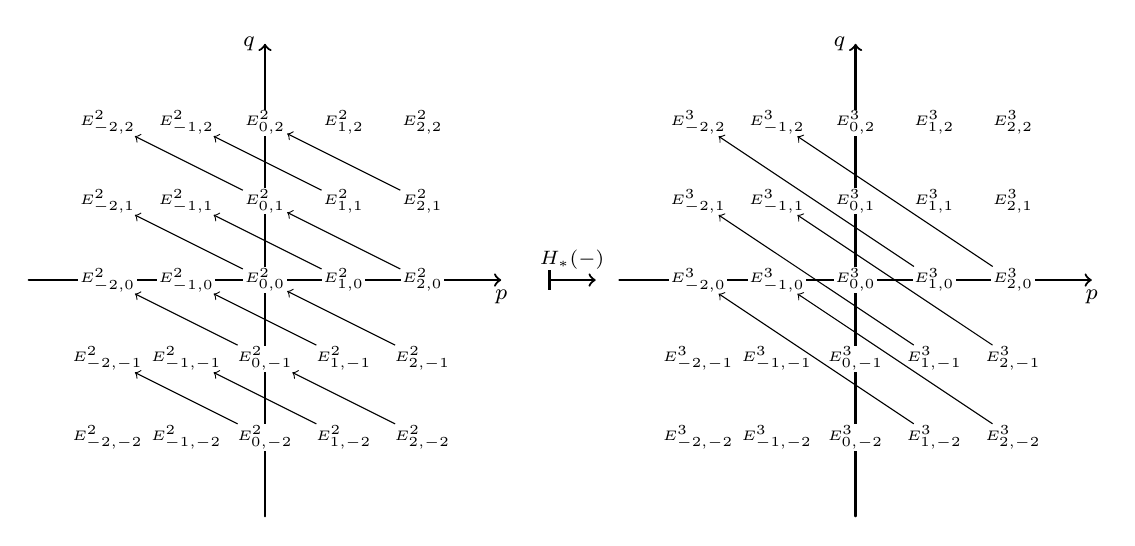
\begin{tikzpicture}[
		pagemember/.style = {
			fill = white, 
			font = \tiny, 
			inner sep = 0.5pt
		}]
		\def\xmin{-3}
		\def\xmax{3}
		\def\ymin{-3}
		\def\ymax{3}
		\begin{scope}
			\coordinate (origin) at (0, 0);
			\draw[spectral sequence/axis] (\xmin, 0) -- (\xmax, 0) node[below] {$p$};
			\draw[spectral sequence/axis] (0, \ymin) -- (0, \ymax) node[left] {$q$};
			\foreach \x [parse = true, evaluate = \x using int(\x)] in {\xmin + 1, ..., \xmax - 1}{
				\foreach \y [parse = true, evaluate = \y using int(\y)] in {\ymin + 1, ..., \ymax - 1}{
					\node[pagemember] (E2-\x-\y) at (\x, \y) {$E^2_{\x, \y}$};
				}
			}
			\foreach \x [parse = true, evaluate = \x using int(\x)] in {\xmin + 3, ..., \xmax - 1}{
				\foreach \y [parse = true, evaluate = \y using int(\y)] in {\ymin + 1, ..., \ymax - 2}{
					\tikzmath{
						int \tx, \ty;
						\tx = \x - 2;
						\ty = \y + 1;
					}
					\draw[->] (E2-\x-\y) -- (E2-\tx-\ty);
				}
			}
		\end{scope}
		\begin{scope}[xshift = 2.5 * \xmax cm]
			\coordinate (origin) at (0, 0);
			\draw[spectral sequence/axis] (\xmin, 0) -- (\xmax, 0) node[below] {$p$};
			\draw[spectral sequence/axis] (0, \ymin) -- (0, \ymax) node[left] {$q$};
			\foreach \x [parse = true, evaluate = \x using int(\x)] in {\xmin + 1, ..., \xmax - 1}{
				\foreach \y [parse = true, evaluate = \y using int(\y)] in {\ymin + 1, ..., \ymax - 1}{
					\node[pagemember] (E3-\x-\y) at (\x, \y) {$E^3_{\x, \y}$};
				}
			}
			\foreach \x [parse = true, evaluate = \x using int(\x)] in {\xmin + 4, ..., \xmax - 1}{
				\foreach \y [parse = true, evaluate = \y using int(\y)] in {\ymin + 1, ..., \ymax - 3}{
					\tikzmath{
						int \tx, \ty;
						\tx = \x - 3;
						\ty = \y + 2;
					}
					\draw[->] (E3-\x-\y) -- (E3-\tx-\ty);
				}
			}
		\end{scope}
		\draw[|->, thick] (1.2 * \xmax, 0) --++(0:.2 * \xmax) node[anchor = south, midway, font = \scriptsize] {$H_*({{-}})$};
	\end{tikzpicture}
	\caption{$E^2$- and $E^3$-pages of a homologically graded spectral sequence}
\end{figure}
\begin{definition}
	We say a spectral sequence is \strong{first quadrant}\index{spectral sequence!first quadrant} if all the groups $E^2_{p, q}$ are trivial whenever $p < 0$ or $q < 0$.
\end{definition}
\begin{figure}[ht]
	\centering
	\tikzsetnextfilename{specseq_firstquadrant}
	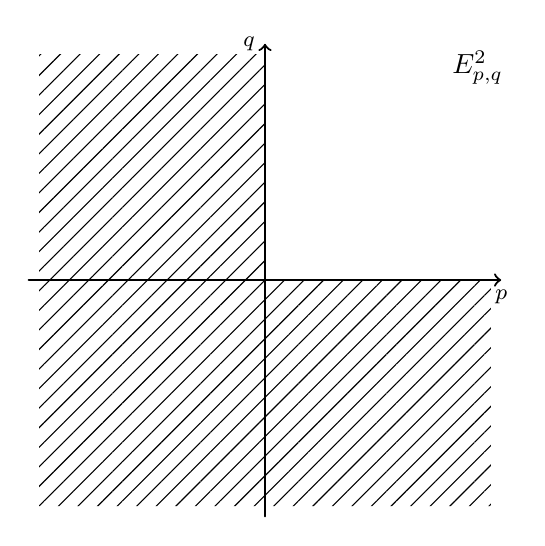
\begin{tikzpicture}[
		shaded/.style = {
			postaction = {
				pattern = {
					Lines[angle = 45, distance = 5pt]
				}
			}
		}]
		\draw[spectral sequence/axis] (-3, 0) -- (3, 0) node[below] {$p$};
		\draw[spectral sequence/axis] (0, -3) -- (0, 3) node[left] {$q$};

		\path[shaded] (0, 0) -- (0, 2.87) -- (-2.87, 2.87) -- (-2.87, -2.87) -- (2.87, -2.87) -- (2.87, 0) -- cycle;
		\node[draw = none, fill = white, inner sep = 2pt, outer sep = 0] at (2.7, 2.7) {$E^2_{p, q}$};
	\end{tikzpicture}
	\caption{A first-quadrant spectral sequence. All potentially nontrivial groups live in the unshaded quadrant.}
\end{figure}
\begin{lemma}
	For a first quadrant spectral sequence $(E^\bullet, d^\bullet, h^\bullet)$ we have $E^r_{p, q} = 0$ if $p < 0$ or $q < 0$ for all $r \geq 2$.
	Moreover, for a given pair $(p, q) \in \Z \times \Z$ the map $h$ induces an isomorphism for all $r > r_0 \coloneq \max(p, q + 1)$, i.e. the groups $E^r_{p, q}$ stabilize as $r \to \infty$.
\end{lemma}
\begin{proof}
	The first statement follows immediately from the existence of $h^\bullet$ by induction on $r$.
	For the second statement, if $r > r_0$, then the target of the differential $d^r\colon E^r_{p, q} \to E^r_{p - r, q + r - 1}$ is trivial since $p - r < 0$, so every element of $E^r_{p, q}$ is a cycle.
	Moreover, the domain of the incoming differential $E^r_{p + r, q - r + 1} \to E^r_{p, q}$ is trivial since $q - r + 1 < 0$, so $E^r_{p, q} \isom H_*(E^r_{p, q}) \isom E^{r + 1}_{p, q}$.
\end{proof}
\begin{definition}
	For a first quadrant spectral sequence $(E^\bullet, d^\bullet, h^\bullet)$ we define its \strong{$E^\infty$-page}\index{$E^\infty$-page} as the bigraded abelian group
	\begin{equation*}
		E^\infty_{p, q} \coloneq E^{r_0(p, q) + 1}_{p, q}
	\end{equation*}
	with $r_0(p, q) \coloneq \max(p, q + 1)$.
	By the previous lemma, $E^\infty_{p, q} \isom E^r_{p, q}$ whenever $r > r_0(p, q)$.
\end{definition}
By a \strong{filtered object}\index{filtered object} $(H, F)$ in an abelian category $\mathcal{A}$ we mean an object $H \in \mathcal{A}$ together with a sequence of inclusions
\begin{equation*}
	0 = F^{-1} \subseteq F^0 \subseteq F^1 \subseteq \ldots \subseteq F^n \subseteq \ldots \subseteq H
\end{equation*}
We will apply this to the category of graded abelian groups and $H = H_*(E; \Z)$.
Notationally, if $(H, F)$ is a filtered object in abelian groups, we write $F^n_m$ for the $n$th object in the filtration associated to the group $H_m$; in other words, $F^0_m \subseteq F^1_m \subseteq \ldots \subseteq H_m$ is the filtration associated to $H_m$.
\begin{definition}
	A first quadrant spectral sequence is said to \strong{converge}\index{convergence!of spectral sequences} to a filtered object in graded abelian groups $(H, F)$ if there is a chosen isomorphism
	\begin{equation*}
		E^\infty_{p, q} \isom F^p_{p + q} / F^{p - 1}_{p + q}
	\end{equation*}
	for all values of $p$ and $q$, and $F^p_n = H_n$ if $p \geq n$.
	In this case, we write $E^2_{p, q} \Rightarrow H$.
\end{definition}
\begin{figure}[ht]
	\centering
	\tikzsetnextfilename{specseq_convergence}
	\begin{tikzpicture}[
			dot/.style = {
				draw,
				fill, 
				circle,
				inner sep = 1pt,
			},
			pin distance = 1em,
			every pin/.style = {
				font = \footnotesize,
			},
			every label/.style = {
				font = \footnotesize,
			},
		]
		\def\maxextent{4}

		\coordinate (Origin) at (0, 0);
		\coordinate (Bottom Right) at (\maxextent, 0);
		\coordinate (Top Left) at (0, \maxextent);
		\coordinate (Y Midway) at ($(Origin)!0.5!(Top Left)$);
		\coordinate (X Midway) at ($(Origin)!0.5!(Bottom Right)$);

		\draw[spectral sequence/axis] (Origin) -- (Bottom Right) node[below] {$p$};
		\draw[spectral sequence/axis] (Origin) -- (Top Left) node[left] {$q$};

		\draw[line width = 0.6pt] (Y Midway) -- (X Midway);

		\node[dot, pin = below left:{$F_0^0 = H_0$}] at (Origin) {};
		\node[dot, "$n$" left, pin = 65:$F_n^0$] at (Y Midway) {};
		\node[dot, pin = 50:$F_n^1 / F_n^0$] at ($(Y Midway)!0.15!(X Midway)$) {};
		\node[dot, pin = 25:$F_n^2 / F_n^1$] at ($(Y Midway)!0.30!(X Midway)$) {};
		\node[inner sep = 0.1pt, circle, fill = white, font = \scriptsize] at ($(Y Midway)!0.45!(X Midway)$) {$\ddots$};
		\node[dot, "$n$" below, pin = above right:{$\overbrace{F_n^n}^{= H_n} / F_n^{n - 1}$}] at (X Midway) {};

		\node[inner sep = 1pt, font = \footnotesize] (Label Node) at (3.5, 3.5) {$E_{p, q}^\infty$};
		\draw[line width = 0.7pt] (Label Node.north west) -- (Label Node.south west) -- (Label Node.south east);
	\end{tikzpicture}
	\caption{Convergence of a first-quadrant spectral sequence.}
\end{figure}
\begin{remark}
	\leavevmode
	\begin{itemize}
		\item Convergence is really a \emph{datum} of isomorphism $E^\infty_{p, q} \isom F^p_{p + q} / F^{p - 1}_{p + q}$ and not a property.
		\item Convergent spectral sequences are often simply encoded as $E^2_{p, q} \Rightarrow H$, but this suppresses not only this data but also the higher pages, the differentials, and the filtration on $H$!
	\end{itemize}
\end{remark}

\subsection{Fibre Sequences}
In order to be able to move onto the definition of the Serre spectral sequence for fibre sequences, let us define exactly what we mean by \enquote{fibre sequence.}
\begin{definition}
	Let $f\colon Y \to X$ be a map of spaces and $x \in X$ a point.
	The \strong{homotopy fibre}\index{homotopy fibre} $\hofib_x(f)$ of $f$ at $x$ is the space
	\begin{equation*}
		\hofib_x(f) \coloneq P_x X \times_X Y
	\end{equation*}
	where $P_x X = \{\gamma\colon I \to X \mid \gamma(1) = x\}$ is the \strong{based path space}\index{path space} of $X$.
	It comes with the evaluation at 0 map $\ev_0\colon P_x X \to X,\ \gamma \mapsto \gamma(0)$.
	In fact, it is the pullback
	\begin{equation*}
		\begin{tikzcd}
			\hofib_x(f)
					\ar[r]
					\ar[d]
					\ar[dr, phantom, "\lrcorner" very near start]
				& P_x X
					\ar[d, "\ev_0"]
			\\
			Y 
					\ar[r, "f"]
				& X
		\end{tikzcd}
	\end{equation*}
\end{definition}
In words, $\hofib_x(f)$ is the space of pairs $(\gamma, y)$ where $y \in Y$ is a point and $\gamma$ is a path from $f(y)$ to $x$.
We note that $P_x X$ is contractible via the homotopy
\begin{align*}
	H\colon P_x X \times I &\to P_x X \\
	(\gamma, t) &\mapsto (s \mapsto \gamma((1 - t)s + t))
\end{align*}
\begin{example}
	If $* \xto{f} X$ is the inclusion of any point, then $\hofib_x(f) = \Omega_x X$.
\end{example}
\begin{definition}
	A \strong{fibre sequence of topological spaces} is a sequence $F \xto{i} Y \xto{f} X$, a basepoint $x \in X$, and a homotopy $h\colon F \to X^I$ from the composite $f \circ i$ to the constant map $c_x\colon F \to X$ such that the induced map
	\begin{equation*}
		F \to \hofib_x(f),\ z \mapsto (h(z), i(z))
	\end{equation*}
	is a weak homotopy equivalence.
\end{definition}
\begin{example}\label{expl:fibresequences}
	\leavevmode
	\begin{enumerate}
		\item Let $f\colon Y \to X$ be any continuous map, $x \in X$ a point.
			Then the pair $(\hofib_x(f) \xto{i} Y \xto{f} X, h)$ where $i(\gamma, y) \coloneq y$ is a fibre sequence since by construction the map $\hofib_x(f) \to \hofib_x(f)$ is just the identity.
	\end{enumerate}
\end{example}
Every fibre sequence is equivalent to such an example in the following sense:
Given $(F \xto{i} Y \xto{f} X)$, there is a commutative diagram
\begin{equation*}
	\begin{tikzcd}
		F
				\ar[r, "\htpyeqv_w"]
				\ar[d]
			& \hofib_x(f)
				\ar[d]
		\\
		Y
				\ar[r, equal, "\id_Y"]
				\ar[d, "f"]
			& Y
				\ar[d, "f"]
		\\
		X 
				\ar[r, equal, "\id_X"]
			& X
	\end{tikzcd}
\end{equation*}
an \enquote{equivalence of fibre sequences}.
In particular, $\Omega X \to * \to X$ is a fibre sequence where $h\colon \Omega X \times I \to X$ is the evaluation map.

\strong{Warning:} If one instead chooses $h$ to be the constant homotopy, one does not obtain a fibre sequence (unless $X$ is weakly contractible) because the induced map $\Omega X \to \hofib_x(f) = \Omega X$ is the constant map which is in general not a weak homotopy equivalence.
Hence, the choice of $h$ is important!

\begin{continueexample}{expl:fibresequences}
	\leavevmode
	\begin{enumerate}[start = 2]
		\item For every two spaces $F$ and $X$ and all basepoints $x \in X$, the pair $(F \to F \times X \xto{\pr_X} X, \const)$ is a fibre sequence called the \strong{trivial fibre sequence}\index{trivial fibre sequence}.
			To see this, note that
			\begin{equation*}
				\hofib_x(\pr_X) = F \times P_x X
			\end{equation*}
			with induced map $F \to F \times P_x X,\ y \mapsto (y, \const_x)$ which is a homotopy equivalence as $P_x X$ is contractible.
		\item\label{expl:fibrebundlefibresequence} Let $p\colon E \to B$ be a fibre bundle with fibre $F = p^{-1}(b)$ for some $b \in B$.
			Then the sequence $F \to E \xto{p} B$ together with the constant homotopy is a fibre sequence.
			This is a special case of the next example:
		\item Recall that $p\colon E \to B$ is a \strong{Serre fibration}\index{fibration!Serre} if in every commutative diagram of the form
			\begin{equation*}
				\begin{tikzcd}
					D^n \times \{0\}
							\ar[r]
							\ar[d, hook]
						& E
							\ar[d, "p"]
					\\
					D^n \times I
							\ar[r]
							\ar[ur, dashed]
						& B
				\end{tikzcd}
			\end{equation*}
			a lift $D^n \times I \to E$ exists making the whole diagram commute.
			Given a Serre fibration $p\colon E \to B$ and a point $b \in B$, the sequence $F = p^{-1}(b) \incl E \to B$ together with the constant homotopy is a fibre sequence (the proof of this is exercise \ref{ex:serrefib}).
		\item\label{expl:hopfbundle} As a special case of \ref{expl:fibrebundlefibresequence}, the \strong{Hopf fibration}\index{Hopf fibration} is a fibre bundle
			\begin{equation*}
				S^1 \to S^3 \xto{\eta} S^2
			\end{equation*}
			It arises by letting $S^1 = \Uni(1)$ act on $S^3 \subseteq \C^2$ via
			\begin{equation*}
				\lambda \cdot (x_1, x_2) = (\lambda x_1, \lambda x_2)
			\end{equation*}
			The quotient space of this action is $\CP^1 = S^2$.
		\item The previous example generalizes to fibre bundles
			\begin{equation*}
				S^1 \to S^{2n + 1} \to \CP^n
			\end{equation*}
			with limit case
			\begin{equation*}
				\begin{tikzcd}
					S^1
							\ar[r]
							\ar[d, "\htpyeqv"]
						& S^\infty
							\ar[r]
							\ar[d, "\htpyeqv"]
						& \CP^\infty
							\ar[d, equal]
					\\
					\Omega \CP^\infty
							\ar[r]
						& * 
							\ar[r]
						& \CP^\infty
				\end{tikzcd}
			\end{equation*}
	\end{enumerate}
\end{continueexample}

\subsection{The Serre Spectral Sequence}\lecture{16.10.23}
We are now ready to state the existence of the Serre spectral sequence:
\begin{theorem}[Serre]\index{Serre spectral sequence}
	For every fibre sequence $(F \to Y \to X, h)$ with $X$ simply connected and abelian group $A$ there exists a first quadrant spectral sequence of the form
	\begin{equation}\label{s3:defn}
		E^2_{p, q} = H_p(X; H_q(F; A)) \Rightarrow H_{p + q}(Y; A)
	\end{equation}
\end{theorem}
The expression in \eqref{s3:defn} does not include information about the differentials and higher pages, nor about the filtration on $H_*(Y; A)$ and the identification of its subquotients with the $E^\infty$-page.

% TODO understand this
One edge case is easy to state:
The map
\begin{equation*}
	H_n(F; A) \isom H_0(Y; H_n(F; A)) = E^2_{0, n} \twoheadrightarrow E^\infty_{0, n} \incl H_n(Y; A)
\end{equation*}
agrees with the factorization
\begin{equation*}
	\begin{tikzcd}
		H_n(F; A) 
				\ar[r, two heads]
			& \img \iota_*
				\ar[r, hook]
			& H_n(Y; A)
	\end{tikzcd}
\end{equation*}
with $\iota\colon F \incl Y$ the fibre inclusion.

Before proving the theorem, let us first look at some examples.
\begin{example}\index{Hopf fibration}
	We revisit the Hopf fibration
	\begin{equation*}
		S^1 \incl S^3 \xto{\eta} S^2
	\end{equation*}
	The $E^2$-page of its associated Serre spectral sequence looks like this:
	\begin{equation*}
		\pgfsetlayers{background,main}
		\tikzsetnextfilename{specseq_hopfserrespec}
		\begin{tikzpicture}
			\matrix[
				spectral sequence/page,
				name = m, 
				column sep = {4ex, between origins},
				row 3/.style = {font = \scriptsize}] {
					1 &[-1.9ex] A & 0 & A \\
					0 & A & 0 & A \\
					& 0 & 1 & 2 \\
			};

			\draw[spectral sequence/axis] (m-2-2.south west) -- (m-1-2.north west) -- ++(0, 1.5) node[left] (q) {$q$};
			\draw[spectral sequence/axis] (m-2-2.south west) -- (m-2-4.south east) -- ++(1.5, 0) node[below] (p) {$p$};

			\coordinate (Top Right) at (p |- q);

			\coordinate (Slightly Left of p) at ($(p) - (0.14, 0)$);
			\coordinate (Slightly Below q) at ($(q) - (0, 0.14)$);

			\begin{pgfonlayer}{background}
				% instead of figuring out a difficult path around the page content, we simply shade the whole page, then paint the background behind the page content white
				\draw[spectral sequence/zero region] (m-2-2.south west) rectangle (Slightly Left of p |- Slightly Below q); 
				\fill[white] (m-2-2.south west) rectangle (m-1-4.north east);
			\end{pgfonlayer}

			\node[spectral sequence/page label] at ($(Top Right) - (0.3, 0.3)$) {$E^2_{p, q}$};

			\draw[spectral sequence/differential] (m-2-4) -- (m-1-2); % differential
		\end{tikzpicture}
	\end{equation*}
	There is only one potentially non-zero $d^2$-differential, namely
	\begin{equation*}
		d^2\colon E^2_{2, 0} \to E^2_{0, 1}
	\end{equation*}
	All higher differentials are necessarily trivial for degree reasons.
	Hence, the $E^\infty$-page looks as follows:
	\begin{equation*}
		\tikzsetnextfilename{specseq_hopfserrespec_einfty}
		\pgfsetlayers{background,main}
		\begin{tikzpicture} 
			\matrix[
				spectral sequence/page,
				name = m, 
				column sep = {2.5em, between origins},
				row 3/.style = {font = \scriptsize}] {
					1 &[-0.8ex] \coker d^2 & 0 & A \\
					0 & A & 0 & \ker d^2 \\
					& 0 & 1 & 2 \\
			};

			% since (m-1-2.west) (the $coker d^2$-cell) sticks farther out to the left than (m-2-2.south west), we need to do an intersection to get the real "origin" of the system 
			\coordinate (Origin) at (m-1-2.west |- m-2-2.south west);

			\draw[spectral sequence/axis] (Origin) -- (m-1-2.north west) -- ++(0, 1.5) node[left] (q) {$q$};
			\draw[spectral sequence/axis] (Origin) -- (m-2-4.south east) -- ++(1.5, 0) node[below] (p) {$p$};

			\coordinate (Top Right) at (p |- q);

			\coordinate (Slightly Left of p) at ($(p) - (0.14, 0)$);
			\coordinate (Slightly Below q) at ($(q) - (0, 0.14)$);

			\begin{pgfonlayer}{background}
				\draw[spectral sequence/zero region] (Origin) rectangle (Slightly Left of p |- Slightly Below q); 
				\fill[white] (Origin) rectangle (m-1-4.north -| m-2-4.east);
			\end{pgfonlayer}

			\node[spectral sequence/page label] at ($(Top Right) - (0.3, 0.3)$) {$E^\infty_{p, q}$};
		\end{tikzpicture}
	\end{equation*}
	We know that $H_n(S^3; A) \isom A$ if $n = 0, 3$ and 0 else, so from the $E^\infty$-page we obtain that $H_0(S^3; A) \isom A$, $H_1(S^3; A) \isom \coker d^2$, $H_2(S^3; A) \isom \ker d^2$, and $H_3(S^3; A) \isom A$. 
	Thus, $d^2\colon E^2_{2, 0} \to E^2_{0, 1}$ must be an isomorphism.
\end{example}

\begin{lemma}
	There is a fibre bundle
	\begin{equation*}
		\Uni(n - 1) \xto{i} \Uni(n) \to S^{2n - 1}
	\end{equation*}
	where $\Uni(n)$ denotes the topological group of unitary $(n \times n)$-matrices and $i$ is the standard inclusion which adds a trivial $\C$-summand:
	\begin{equation*}
		i(A) = \begin{pmatrix}
			A & 0 \\
			0 & 1
		\end{pmatrix}
	\end{equation*}
\end{lemma}
\begin{proof}
	The group $\Uni(n)$ acts on $\C^n$ by definition.
	This action restricts to the unit sphere $S^{2n - 1} \subseteq \C^n$.
	Furthermore, this action is transitive because every length 1 vector can be extended to an orthonormal basis.
	Hence, $S^{2n - 1}$ is in bijection with the \enquote{orbit space} $\Uni(n) / \Stab(x)$ for any $x \in S^{2n - 1}$ where $\Stab(x) \coloneq \{A \in \Uni(n) \mid Ax = x\}$ is the \emph{stabilizer} of $x$.
	For $x = (0, \ldots, 0, 1)$, this stabilizer equals $\Uni(n - 1)$.
	We obtain a continuous bijection
	\begin{align*}
		\Uni(n) / \Uni(n - 1) &\to S^{2n - 1} \\
		A \cdot \Uni(n - 1) &\mapsto A \cdot (0, \ldots, 0, 1)
	\end{align*}
	As $\Uni(n) / \Uni(n - 1)$ is quasi-compact and $S^{2n - 1}$ is Hausdorff, this map is a homeomorphism.
	Finally, we use the fact that for a smooth free action of a compact Lie group $G$ on a manifold $M$, the map $M \to M / G$ is always a fibre bundle (in fact a $G$-principal bundle) see \cite[Problem 21-6]{lee_introduction_2012}.
\end{proof}
\begin{example}\label{expl:homology_uni_2}
	We consider the case $n = 2$, i.e. the fibre sequence 
	\begin{equation*}
		S^1 \isom \Uni(1) \to \Uni(2) \to S^3
	\end{equation*}
	Our goal is to compute the homology of $\Uni(2)$ via the Serre spectral sequence, whose $E^2$-page looks as follows:
	\begin{center}
		\pgfsetlayers{background,main}
		\tikzsetnextfilename{specseq_uni_1_2_seq}
		\begin{tikzpicture}
			\matrix[
				spectral sequence/page,
				name = m, 
				column sep = {3ex, between origins},
				row 3/.style = {font = \scriptsize}
				] {
					1 &[-1ex] \Z 	& 0 & 0 & \Z \\
					0 & \Z 			& 0 & 0 & \Z \\
					& 0 			& 1 & 2 & 3  \\
			};

			\draw[spectral sequence/axis] (m-2-2.south west) -- (m-1-2.north west) -- ++(0, 1.5) node[left] (q) {$q$};
			\draw[spectral sequence/axis] (m-2-2.south west) -- (m-2-5.south east) -- ++(1.5, 0) node[below] (p) {$p$};

			\coordinate (Top Right) at (p |- q);

			\coordinate (Slightly Left of p) at ($(p) - (0.14, 0)$);
			\coordinate (Slightly Below q) at ($(q) - (0, 0.14)$);

			\begin{pgfonlayer}{background}
				% instead of figuring out a difficult path around the page content, we simply shade the whole page, then paint the background behind the page content white
				\draw[spectral sequence/zero region] (m-2-2.south west) rectangle (Slightly Left of p |- Slightly Below q); 
				\fill[white] (m-2-2.south west) rectangle (m-1-5.north east);
			\end{pgfonlayer}

			\node[spectral sequence/page label] at ($(Top Right) - (0.3, 0.3)$) {$E^2_{p, q}$};
		\end{tikzpicture} \\
		$E^2_{p, q} = H_p(S^3; H_q(\Uni(1); \Z))$
	\end{center}
	All differentials on all pages have to be trivial for degree reasons.
	Hence the $E^\infty$-page equals the $E^2$-page.
	Moreover, every antidiagonal has at most one non-trivial term, so we can read off that
	\begin{equation*}
		H_n(\Uni(2); \Z) \isom \begin{cases}
			\Z & n = 0, 1, 3, 4 \\
			0  & \text{else}
		\end{cases}
	\end{equation*}
	In fact, one can show that $\Uni(2)$ is homeomorphic to $S^3 \times \Uni(1)$, so this result could also be derived from the Künneth theorem.
\end{example}
\begin{example}\label{expl:homology_uni_3}
	Next, we consider the fibre sequence 
	\begin{equation*}
		\Uni(2) \to \Uni(3) \to S^5
	\end{equation*}
	which has Serre spectral sequence $E^2$-page of the form
	\begin{center}
		\pgfsetlayers{background,main}
		\tikzsetnextfilename{specseq_uni_2_3_seq}
		\begin{tikzpicture}
			\matrix[
				spectral sequence/page,
				name = m, 
				column sep = {2ex, between origins},
				row 6/.style = {font = \scriptsize}] {
					4 &[-0.7ex] \Z & & & & & \Z \\
					3 & \Z & & & & & \Z \\
					2 & 0 & & & & & 0 \\
					1 & \Z & & & & & \Z \\
					0 & \Z & & & & & \Z \\
					& 0 & 1 & 2 & 3 & 4 & 5 \\
			};

			\draw[spectral sequence/axis] (m-5-2.south west) -- (m-1-2.north west) -- ++(0, 1) node[left] (q) {$q$};
			\draw[spectral sequence/axis] (m-5-2.south west) -- (m-5-7.south east) -- ++(1.5, 0) node[below] (p) {$p$};

			\coordinate (Top Right) at (p |- q);

			\coordinate (Slightly Left of p) at ($(p) - (0.14, 0)$);
			\coordinate (Slightly Below q) at ($(q) - (0, 0.14)$);

			\begin{pgfonlayer}{background}
				\draw[spectral sequence/zero region] (m-5-2.south west) rectangle (Slightly Left of p |- Slightly Below q); 
				\fill[white] (m-5-2.south west) rectangle (m-1-2.north east);
				\fill[white] (m-5-7.south west) rectangle (m-1-7.north east);
			\end{pgfonlayer}

			\node[spectral sequence/page label] at ($(Top Right) - (0.3, 0.3)$) {$E^2_{p, q}$};

			\draw[spectral sequence/differential] (m-5-7) -- node[commutative diagrams/every label, inner sep = 1pt, fill = white, swap] {$d^5$} (m-1-2);
		\end{tikzpicture} \\
		$E^2_{p, q} = H_p(S^5; H_q(\Uni(2); \Z))$
	\end{center}
	The first potentially non-trivial differential is a $d^5$, the map
	\begin{equation*}
		d^5\colon \underbrace{E^5_{5, 0}}_{\isom \Z} \to \underbrace{E^5_{0, 4}}_{\isom \Z}
	\end{equation*}
	At this point, we cannot decide what this differential is (at least not without resorting to tools like Poincaré duality).
	All higher differentials are again trivial for degree reasons and all filtrations collapse to at most one entry, so we obtain
	\begin{equation*}
		H_n(\Uni(3); \Z) \isom \begin{cases}
			\Z 			& n = 0, 1, 3, 6, 8, 9 \\
			\coker d^5 	& n = 4 \\
			\ker d^5 	& n = 5 \\
			0 			& \text{else}
		\end{cases}
	\end{equation*}
	This example illustrates a typical situation, namely that one can often not fully determine all differentials but still deduce a lot of information.
	We will soon see that $d^5 = 0$ and hence $H_4(\Uni(3); \Z) \isom H_5(\Uni(3); \Z) \isom \Z$.
\end{example}
\begin{example}\label{expl:homology_uni_4}
	We consider 
	\begin{equation*}
		\Uni(3) \to \Uni(4) \to S^7
	\end{equation*}
	and its associated Serre spectral sequence which has $E^2$-page
	\begin{center}
		\pgfsetlayers{background,main}
		\tikzsetnextfilename{specseq_uni_3_4_seq}
		\begin{tikzpicture}
			\matrix[
				spectral sequence/page,
				name = m, 
				column sep = {2ex, between origins},
				row 11/.style = {font = \scriptsize}] {
					9 &[-0.6ex] \Z & & & & & & & \Z \\
					8 & \Z & & & & & & & \Z \\
					7 & 0 & & & & & & & 0 \\
					6 & \Z & & & & & & & \Z \\
					5 & ? & & & & & & & ? \\
					4 & ? & & & & & & & ? \\
					3 & \Z & & & & & & & \Z \\
					2 & 0 & & & & & & & 0 \\
					1 & \Z & & & & & & & \Z \\
					0 & \Z & & & & & & & \Z \\
					& 0 & 1 & 2 & 3 & 4 & 5 & 6 & 7 \\
			};

			\draw[spectral sequence/axis] (m-10-2.south west) -- (m-1-2.north west) -- ++(0, .8) node[left] (q) {$q$};
			\draw[spectral sequence/axis] (m-10-2.south west) -- (m-10-9.south east) -- ++(1.5, 0) node[below] (p) {$p$};

			\coordinate (Top Right) at (p |- q);

			\coordinate (Slightly Left of p) at ($(p) - (0.14, 0)$);
			\coordinate (Slightly Below q) at ($(q) - (0, 0.14)$);

			\begin{pgfonlayer}{background}
				\draw[spectral sequence/zero region] (m-10-2.south west) rectangle (Slightly Left of p |- Slightly Below q); 
				\fill[white] (m-10-2.south west) rectangle (m-1-2.north east);
				\fill[white] (m-10-9.south west) rectangle (m-1-9.north east);
			\end{pgfonlayer}

			\node[spectral sequence/page label] at ($(Top Right) - (0.3, 0.3)$) {$E^2_{p, q}$};

			\draw[spectral sequence/differential] (m-10-9) -- node[commutative diagrams/every label, inner sep = 1pt, fill = white, swap] {$d^7$} (m-4-2);
			\draw[spectral sequence/differential] (m-7-9) -- node[commutative diagrams/every label, inner sep = 1pt, fill = white, swap] {$d^7$} (m-1-2);
		\end{tikzpicture} \\
		$E^2_{p, q} = H_p(S^7; H_q(\Uni(3); \Z))$
	\end{center}
	The only possible non-trivial differentials are
	\begin{align*}
		d^7\colon E^7_{7, 0} &\to E^7_{0, 6} \\
		d^7\colon E^7_{7, 5} &\to E^7_{0, 9}
	\end{align*}
	which we cannot compute at this point.
	Nevertheless we can still deduce a lot, for example that
	\begin{equation*}
		H_n(\Uni(4); \Z) \isom \begin{cases}
			\Z 					& n = 0, 1, 3 \\
			H_4(\Uni(3); \Z) 	& n = 4 \\
			H_5(\Uni(3); \Z) 	& n = 5 \\
			0 					& n = 2
		\end{cases}
	\end{equation*}
	and that there is a short exact sequence
	\begin{equation*}
		0 \to \Z \to H_8(\Uni(4); \Z) \to \Z \to 0
	\end{equation*}
	which splits to yield $H_8(\Uni(4); \Z) \isom \Z \dsum \Z$.
\end{example}

In the previous examples we used the Serre spectral sequence to compute the homology of the total space of the fibre sequence.
We now show that it can be used to compute the homology of the basespace or fibre.
\begin{example}\label{expl:homology_cp_n}
	We consider the fibre sequence 
	\begin{equation*}
		S^1 \to S^{2n + 1} \to \CP^n
	\end{equation*}
	for $n \geq 2$.
	Let us pretend that we do not know $H_*(\CP^n)$.
	The only thing we can say about the $E^2$-page of the associated Serre spectral sequence a priori is then that its bottom-left corner looks as follows:
	\begin{center}
		\tikzsetnextfilename{specseq_cpn_initial}
		\begin{tikzpicture}
			\matrix[
				spectral sequence/page,
				name = m, 
				column sep = {2.5ex, between origins},
				row 3/.style = {font = \scriptsize}] {
					1 &[-0.7ex]\Z & ? & ? & \cdots \\
					0 & \Z & ? & ? & \cdots \\
					& 0 & 1 & 2 & \ldots \\
			};

			\draw[spectral sequence/axis] (m-2-2.south west) -- (m-1-2.north west) -- ++(0, 1) node[left] (q) {$q$};
			\draw[spectral sequence/axis] (m-2-2.south west) -- (m-2-5.south east) -- ++(1, 0) node[below] (p) {$p$};

			\coordinate (Top Right) at (p |- q);

			\coordinate (Slightly Left of p) at ($(p) - (0.12, 0)$);
			\coordinate (Slightly Below q) at ($(q) - (0, 0.14)$);

			\draw[spectral sequence/zero region] (m-1-2.north west) rectangle (Slightly Left of p |- Slightly Below q); 

			\node[spectral sequence/page label] at ($(Top Right) - (0.3, 0.3)$) {$E^2_{p, q}$};
		\end{tikzpicture} \\ 
		$E^2_{p, q} = H_p(\CP^n; H_q(S^1; \Z))$
	\end{center}
	Since $H_1(S^{2n + 1}; \Z) = 0$, there must be a surjective $d^2$-differential $d^2\colon E^2_{2, 0} \to E^2_{0, 1}$.
	As $H_2(S^{2n + 1}; \Z) = 0$, this differential must be injective, so $\Z \isom E^2_{2, 0} = H_2(\CP^n; H_0(S^1; \Z)) = H_2(\CP^n; \Z)$.
	Furthermore, we see that $H_1(\CP^n; \Z) = E^2_{1, 0} = 0$.
	This implies that $E^2_{1, 1} = H_1(\CP^n; H_1(S^1; \Z)) = 0$ and $E^2_{2, 1} = H_2(\CP^n; H_1(S^1; \Z)) \isom \Z$ as $H_1(S^1; \Z) \isom \Z$.
	Since we also have $H_3(S^{2n + 1}; \Z) = 0$, the same argument to deduce that $d^2\colon E^2_{4, 0} = H_4(\CP^n; H_0(S^1; \Z)) \to E^2_{2, 2} \isom \Z$ must be an isomorphism, hence $H_4(\CP^n; \Z) \isom \Z$.
	This can be iterated until we get the following picture:
	\begin{center}
		\tikzsetnextfilename{specseq_cpn_intermediate}
		\begin{tikzpicture}
			\matrix[
				spectral sequence/page,
				name = m, 
				column sep = {2.5em, between origins},
				row 3/.style = {font = \scriptsize}] {
					1 &[-1.8em]\Z 	& 0 	& \Z 	& 0		& \cdots	  	& \textcolor{highlightcol}{\Z} & 0 		& ? 		& \cdots\\
					0 & \Z 			& 0 	& \Z 	& 0		& \cdots	 	& \Z & 0 		& ? 		& \cdots \\
					& 0 			& 1 	& 2 	& 3 	& \cdots 	 	& 2n & 2n + 1 	& 2n + 2 	& \cdots \\
			};

			\draw[spectral sequence/axis] (m-2-2.south west) -- (m-1-2.north west) -- ++(0, 1) node[left] (q) {$q$};
			\draw[spectral sequence/axis] (m-2-2.south west) -- (m-2-10.south east) -- ++(1, 0) node[below] (p) {$p$};

			\coordinate (Top Right) at (p |- q);

			\coordinate (Slightly Left of p) at ($(p) - (0.12, 0)$);
			\coordinate (Slightly Below q) at ($(q) - (0, 0.14)$);

			\draw[spectral sequence/zero region] (m-1-2.north west) rectangle (Slightly Left of p |- Slightly Below q); 

			\node[spectral sequence/page label] at ($(Top Right) - (0.3, 0.3)$) {$E^2_{p, q}$};

			\draw[spectral sequence/differential] (m-2-4) -- node[commutative diagrams/every label, inner sep = 1pt, fill = white, swap] {$\isom$} (m-1-2);
			\draw[spectral sequence/differential] (m-2-6) -- node[commutative diagrams/every label, inner sep = 1pt, fill = white, swap] {$\isom$} (m-1-4);
		\end{tikzpicture}
	\end{center}
	Since $H_{2n + 1}(S^{2n + 1}; \Z) \isom \Z$, we cannot conclude that the $\textcolor{highlightcol}{\Z}$ in bidegree $(2n, 1)$ must be the image of a differential.
	There are then two possibilities:
	\begin{enumerate}
		\item $d^2\colon E^2_{2n + 2, 0} \to E^2_{2n, 1}$ is trivial.
			This implies $E^2_{2n + 2, 0} = 0$ and by induction that $E^2_{p, q} = 0$ for all $p > 2n$; or
		\item $d^2\colon E^2_{2n + 2, 0} \to E^2_{2n, 1} \isom \Z$ is non-zero.
			Since its cokernel is isomorphic to the lowest term of the filtration on $H_{2n + 1}(S^{2n + 1}; \Z) \isom \Z$, this forces $d^2$ to be surjective as no $\Zn{n}$ with $n > 1$ embeds into $\Z$.
			We obtain the following pattern infinite pattern:
			\begin{center}
				\tikzsetnextfilename{specseq_cpn_final_impossible}
				\begin{tikzpicture}
					\matrix[
						spectral sequence/page,
						name = m, 
						column sep = {2.5em, between origins},
						row 3/.style = {font = \scriptsize}] {
							1 &[-1.8em]\Z 	& 0 	& \Z 	& 0		& \cdots	  	& \textcolor{highlightcol}{\Z} & 0 		& \textcolor{highlightcol}{\Z} & 0		& \cdots\\
							0 & \Z 			& 0 	& \Z 	& 0		& \cdots	 	& \Z & 0 		& \textcolor{highlightcol}{\Z} 	& 0 	& \cdots \\
							& 0 			& 1 	& 2 	& 3 	& \cdots 	 	& 2n & 2n + 1 	& 2n + 2 	& 2n + 3 & \cdots \\
					};

					\draw[spectral sequence/axis] (m-2-2.south west) -- (m-1-2.north west) -- ++(0, 1) node[left] (q) {$q$};
					\draw[spectral sequence/axis] (m-2-2.south west) -- (m-2-11.south east) -- ++(1, 0) node[below] (p) {$p$};

					\coordinate (Top Right) at (p |- q);

					\coordinate (Slightly Left of p) at ($(p) - (0.12, 0)$);
					\coordinate (Slightly Below q) at ($(q) - (0, 0.14)$);

					\draw[spectral sequence/zero region] (m-1-2.north west) rectangle (Slightly Left of p |- Slightly Below q); 

					\node[spectral sequence/page label] at ($(Top Right) - (0.3, 0.3)$) {$E^2_{p, q}$};

					\draw[spectral sequence/differential] (m-2-4) -- node[commutative diagrams/every label, inner sep = 1pt, fill = white, swap] {$\isom$} (m-1-2);
					\draw[spectral sequence/differential] (m-2-6) -- node[commutative diagrams/every label, inner sep = 1pt, fill = white, swap] {$\isom$} (m-1-4);
					\draw[spectral sequence/differential, highlightcol] (m-2-9) -- node[commutative diagrams/every label, inner sep = 1pt, fill = white, swap] {$\isom$} (m-1-7);
					\draw[spectral sequence/differential, highlightcol] (m-2-11) -- node[commutative diagrams/every label, inner sep = 1pt, fill = white, swap] {$\isom$} (m-1-9);
				\end{tikzpicture}
			\end{center}
			This can be ruled out using e.g. that $\CP^n$ is $2n$-dimensional CW-complex and therefore $H_k(\CP^n; \Z) = 0$ for $k > 2n$.
	\end{enumerate}
	We thus obtain 
	\begin{equation*}
		H_k(\CP^n; \Z) \isom \begin{cases}
			\Z & k = 2, 4, \ldots, 2n \\
			0  & \text{else}
		\end{cases}
	\end{equation*}
\end{example}

\lecture{20.10.23}
Next, we turn to an exercise of how the Serre spectral sequence can be used to compute the homology of the fibre.
\begin{example}\label{expl:homology_loops_s_3}
	We consider the fibre sequence
	\begin{equation*}
		\Omega S^3 \to * \to S^3
	\end{equation*}
	The $E^2$-page of its associated Serre spectral sequence looks like this:
	\begin{center}
		\pgfsetlayers{background,main}
		\tikzsetnextfilename{specseq_loop_s_3_initial}
		\begin{tikzpicture}
			\matrix[
				spectral sequence/page,
				name = m, 
				column sep = {2.5ex, between origins},
				row 5/.style = {font = \scriptsize}] {
					\vdotswithin{1} & \vdotswithin{\Z}  & & & \vdotswithin{\Z} \\
					2 & ?  & & & ? \\
					1 & ?  & & & ? \\
					0 & \Z & & & \Z \\ 
					& 0 & 1 & 2 & 3 \\
			};

			\draw[spectral sequence/axis] (m-4-2.south west) -- (m-1-2.north west) -- ++(0, 1) node[left] (q) {$q$};
			\draw[spectral sequence/axis] (m-4-2.south west) -- (m-4-5.south east) -- ++(1.5, 0) node[below] (p) {$p$};

			\coordinate (Top Right) at (p |- q);

			\coordinate (Slightly Left of p) at ($(p) - (0.14, 0)$);
			\coordinate (Slightly Below q) at ($(q) - (0, 0.14)$);

			\begin{pgfonlayer}{background}
				\draw[spectral sequence/zero region] (m-4-2.south west) rectangle (Slightly Left of p |- Slightly Below q); 
				\fill[white] (m-4-2.south west) rectangle (m-1-2.north east);
				\fill[white] (m-4-5.south west) rectangle (m-1-5.north east);
			\end{pgfonlayer}

			\node[spectral sequence/page label] at ($(Top Right) - (0.3, 0.3)$) {$E^2_{p, q}$};

			\draw[spectral sequence/differential] (m-4-5) -- node[commutative diagrams/every label, inner sep = 1pt, fill = white, swap] {$d^3$} (m-2-2);
		\end{tikzpicture} \\
		$E^2_{p, q} = H_p(S^3; H_q(\Omega S^3; \Z))$
	\end{center}
	The homology groups of the point are trivial in positive degrees, so we must have $E^\infty_{p, q} = 0$ unless $p = q = 0$.
	The only non-trivial differentials are $d^3$'s, so we conclude that $d^3\colon E^3_{3, q} \to E^3_{0, q + 2}$ must be an isomorphism for all $q \in \N$.
	As $E^3_{3, q} \isom H_3(S^3; H_q(\Omega S^3; \Z)) \isom H_q(\Omega S^3; \Z)$ as well as $E^3_{0, q + 2} \isom H_0(S^3; H_{q + 2}(\Omega S^3; \Z)) \isom H_{q + 2}(\Omega S^3; \Z)$ and finally $H_0(\Omega S^3; \Z) \isom \Z$, this implies that $H_k(\Omega S^3; \Z) \isom \Z$ if $k$ is even and 0 else, and the $E^3$-page looks like this:
	\begin{center}
		\pgfsetlayers{background,main}
		\tikzsetnextfilename{specseq_loop_s_3_final}
		\begin{tikzpicture}
			\matrix[
				spectral sequence/page,
				name = m, 
				column sep = {2.5ex, between origins},
				row 6/.style = {font = \scriptsize}] {
					\vdotswithin{1} & \vdotswithin{\Z}  & & & \vdotswithin{\Z} \\
					3 & 0  & & & 0 \\
					2 & \Z  & & & \Z \\
					1 & 0  & & & 0 \\
					0 & \Z & & & \Z \\ 
					& 0 & 1 & 2 & 3 \\
			};

			\draw[spectral sequence/axis] (m-5-2.south west) -- (m-1-2.north west) -- ++(0, 1) node[left] (q) {$q$};
			\draw[spectral sequence/axis] (m-5-2.south west) -- (m-5-5.south east) -- ++(1.5, 0) node[below] (p) {$p$};

			\coordinate (Top Right) at (p |- q);

			\coordinate (Slightly Left of p) at ($(p) - (0.14, 0)$);
			\coordinate (Slightly Below q) at ($(q) - (0, 0.14)$);

			\begin{pgfonlayer}{background}
				\draw[spectral sequence/zero region] (m-5-2.south west) rectangle (Slightly Left of p |- Slightly Below q); 
				\fill[white] (m-5-2.south west) rectangle (m-1-2.north east);
				\fill[white] (m-5-5.south west) rectangle (m-1-5.north east);
			\end{pgfonlayer}

			\node[spectral sequence/page label] at ($(Top Right) - (0.3, 0.3)$) {$E^3_{p, q}$};

			\draw[spectral sequence/differential] (m-5-5) -- node[commutative diagrams/every label, inner sep = 1pt, fill = white, swap] {$\isom$} (m-3-2);
			\draw[spectral sequence/differential] (m-3-5) -- node[commutative diagrams/every label, inner sep = 1pt, fill = white, swap] {$\isom$} (m-1-2);
		\end{tikzpicture}
	\end{center}
	In particular, we see that $\Omega S^3$ is infinite-dimensional.
\end{example}

We now discuss the cohomological version of the Serre spectral sequence and its multiplicative structure.
The multiplication also helps in determining the differentials, for example for the spectral sequences computing (co)homology of unitary groups.
\begin{definition}
	A \strong{cohomologically-graded spectral sequence}\index{spectral sequence!cohomologically graded}	is a triple $(E_\bullet, d_\bullet, h_\bullet)$ where
	\begin{itemize}
		\item $(E_r)_{r \geq 2}$ is a sequence of bigraded abelian groups,
		\item $d_r\colon E_r \to E_r$ is a sequence of differentials (satisfying $d_r^2 = 0$) of bidegree $(r, 1 - r)$, and
		\item $h_r\colon H_*(E_r) \to E_{r + 1}$ is a sequence of bigrading-preserving isomorphisms.
	\end{itemize}
\end{definition}
As before we define what it means for a spectral sequence to be \strong{first quadrant}\index{spectral sequence!first quadrant} (namely $E^{p, q}_2 = 0$ if $p < 0$ or $q < 0$) and the \strong{$E^\infty$-page}\index{$E^\infty$-page}.
For convergence, we consider descending filtrations $H = F_0 \supseteq F_1 \supseteq \cdots$ instead of the ascending filtrations $0 = F^{-1} \subseteq F_0 \subseteq \cdots \subseteq H$ used in the homologically graded case.
\begin{definition}
	A cohomological first quadrant spectral sequence is said to \strong{converge}\index{convergence!of spectral sequences} to a filtered object $(H, F)$ in graded abelian groups if there are isomorphisms $E^{p, q}_\infty \isom F^{p + q}_p / F^{p + q}_{p + 1}$ for all $p, q$ and if $F^n_p = 0$ if $p \geq n$.
	As before, we write $E^{p, q}_2 \Rightarrow H$.
\end{definition}
\begin{definition}
	A (\strong{commutative}) \strong{multiplicative structure}\index{multiplicative structure!on a spectral sequence} on a cohomologically graded spectral sequence $(E_\bullet, d_\bullet, h_\bullet)$ is a bigraded (commutative) ring structure on $E_\bullet$, i.e. associative multiplication maps
	\begin{equation*}
		E_r^{p, q} \tensor E_r^{p', q'} \to E_r^{p + p', q + q'}
	\end{equation*}
	such that $d_r\colon E_r \to E_r$ is a \emph{graded derivation}\index{graded derivation}, that is to say
	\begin{equation*}
		d_r(x \cdot y) = d_r(x) \cdot y + (-1)^{p + q} x \cdot d_r(y)
	\end{equation*}
	for all $x$ in bidegree $(p, q)$ and all $y$.
	Commutativity here is meant in the graded sense: $x \cdot y$ = $(-1)^{(p + q)(p' + q')} y \cdot x$.

	As a result, each $H_*(E_r)$ is a bigraded ring and we accordingly require the maps $h_\bullet\colon H_*(E_\bullet) \xto{\isom} E_{\bullet + 1}$ to be isomorphisms of bigraded rings.
	Furthermore, the $E_\infty$-page also inherits the structure of a (commutative) bigraded ring.
\end{definition}
\begin{definition}\index{multiplicative filtration}
	A filtration $\cdots \subseteq F_n \subseteq \cdots \subseteq F_1 \subseteq F_0 = H$ on a graded ring $H$ is said to be \strong{multiplicative} or \strong{compatible with the multiplicative structure} if $F_s \cdot F_t \subseteq F_{s + t}$.
	We say that $(H, F)$ is a \strong{filtered graded ring}\index{filtered graded ring}.
\end{definition}
It follows that the associated graded group $\bigdsum_p F_p / F_{p + 1}$ of a filtered graded (commutative) ring is a bigraded (commutative) ring.

\begin{definition}
	A multiplicative first quadrant spectral sequence $(E_\bullet, d_\bullet, h_\bullet)$ is said to \strong{converge}\index{convergence!of spectral sequences} to a filtered graded ring $(H, F)$ if it converges additively and the chosen isomorphisms $E_\infty^{p, q} \isom F^{p + q}_p / F^{p + q}_{p + 1}$ are compatible with the graded ring structure.
\end{definition}
\begin{theorem}[Serre]\index{Serre spectral sequence}
	For every fibre sequence of spaces $(F \to Y \to X, h)$ with simply connected base space $X$ and every abelian group $A$ there exists a first quadrant spectral sequence of the form
	\begin{equation*}
		E^{p, q}_2 = H^p(X; H^q(F; A)) \Rightarrow H^{p + q}(Y; A)
	\end{equation*}
	If $A = R$ is a (commutative) ring, then the spectral sequence and its convergence are multiplicative where on the $E_2$-page the multiplication is given by $(-1)^{q \cdot p'}$ times the composite 
	\begin{equation*}
		\begin{tikzcd}
			H^p(X; H^q(F; R)) \tensor_R H^{p'}(X; H^{q'}(F; R))
					\ar[d]
			\\
			H^{p + p'}(X; H^q(F; R) \tensor_R H^{q'}(F; R))
					\ar[d]
			\\
			H^{p + p'}(X; H^{q + q'}(F; R))
		\end{tikzcd}
	\end{equation*}
\end{theorem}
\begin{note}
	If $H^*(F; R)$ or $H^*(X; R)$ is flat (e.g. free) and of finite type over $R$, then the $E_2$-page is isomorphic to the graded tensor product of $H^*(X; R)$ and $H^*(F; R)$.
\end{note}
\begin{example}
	We reconsider the fibre sequence
	\begin{equation*}
		\Uni(1) \to \Uni(2) \to S^3
	\end{equation*}
	from \ref{expl:homology_uni_2}. 
	As for homology, there can be no non-trivial differentials in the associated Serre spectral sequence for degree reasons.
	Let $x_1 \in H^1(\Uni(1); \Z)$ and $x_3 \in H^3(S^3; \Z)$ be generators.
	As a graded ring, the $E_2$-page and thus also the $E_\infty$-page are isomorphic to $H^*(S^3; \Z) \tensor_{\Z} H^*(\Uni(1); \Z)$.
	Then $H^*(\Uni(1); \Z) \isom \Lambda(x_1)$ and $H^*(S^3; \Z) \isom \Lambda(x_3)$ where $\Lambda(M)$ denotes the \emph{exterior algebra}\index{exterior algebra} on a set $M$, i.e. the free algebra on $M$ modulo the relations $x_i x_j = -x_j x_i$ and $x_i^2 = 0$ for all $x_i, x_j \in M$.
	Hence, the $E_2$-page is the exterior algebra $\Lambda(x_1, x_3)$ and the $\Z$ in bidegree $(3, 1)$ is spanned by $x_1 x_3$, so we obtain the following picture:
	\begin{center}
		\pgfsetlayers{background,main}
		\tikzsetnextfilename{specseq_uni_1_2_cohom_seq}
		\begin{tikzpicture}
			\matrix[
				spectral sequence/page,
				name = m, 
				column sep = {2em, between origins},
				row 3/.style = {font = \scriptsize}
				] {
					1 &[-0.8em] \Z x_1 	& 0 & 0 & \Z x_1 x_3 \\
					0 & \Z 			& 0 & 0 & \Z x_3 \\
					& 0 			& 1 & 2 & 3  \\
			};

			\coordinate (Origin) at (m-1-2.west |- m-2-5.south);

			\draw[spectral sequence/axis] (Origin) -- (m-1-2.north west) -- ++(0, 1.5) node[left] (q) {$q$};
			\draw[spectral sequence/axis] (Origin) -- (m-2-5.south east) -- ++(1.5, 0) node[below] (p) {$p$};

			\coordinate (Top Right) at (p |- q);

			\coordinate (Slightly Left of p) at ($(p) - (0.14, 0)$);
			\coordinate (Slightly Below q) at ($(q) - (0, 0.14)$);

			\begin{pgfonlayer}{background}
				\draw[spectral sequence/zero region] (Origin) rectangle (Slightly Left of p |- Slightly Below q); 
				\fill[white] (Origin) rectangle (m-1-5.north east);
			\end{pgfonlayer}

			\node[spectral sequence/page label] at ($(Top Right) - (0.3, 0.3)$) {$E_2^{p, q}$};
		\end{tikzpicture} \\
		$E_2^{p, q} = H^p(S^3; H^q(\Uni(1); \Z))$
	\end{center}
	The filtration collapses degree-wise, so $H^*(\Uni(2); \Z)$ is exterior on classes $x_1 \in H^1(\Uni(2); \Z)$ and $x_3 \in H^3(\Uni(2); \Z)$ that are uniquely determined by the spectral sequence.
\end{example}
\begin{example}
	We move on to the fibre sequence 
	\begin{equation*}
		\Uni(2) \to \Uni(3) \to S^5
	\end{equation*}
	from example \ref{expl:homology_uni_3}.
	Again, the $E_2$-page of the associated spectral sequence is given by $H^*(S^5; \Z) \tensor_{\Z} H^*(\Uni(2); \Z) \isom \Lambda(x_1, x_3, x_5)$ where $x_5 \in H^5(S^5; \Z)$ is a generator, and there is only one possibly non-trivial differential $d_5\colon E_5^{0, 4} \to E_5^{5, 0}$, so we obtain the following picture:
	\begin{center}
		\pgfsetlayers{background,main}
		\tikzsetnextfilename{specseq_uni_2_3_cohom_seq}
		\begin{tikzpicture}
			\matrix[
				spectral sequence/page,
				name = m, 
				column sep = {2.2em, between origins},
				row 6/.style = {font = \scriptsize}] {
					4 &[-0.7ex] \Z x_1 x_3 & & & & & \Z x_1 x_3 x_5 \\
					3 & \Z x_3 & & & & & \Z x_3 x_5 \\
					2 & 0 & & & & & 0 \\
					1 & \Z x_1 & & & & & \Z x_1 x_5 \\
					0 & \Z & & & & & \Z x_5 \\
					& 0 & 1 & 2 & 3 & 4 & 5 \\
			};

			\coordinate (Origin) at (m-1-2.west |- m-5-7.south);

			\draw[spectral sequence/axis] (Origin) -- (m-1-2.north west) -- ++(0, 1) node[left] (q) {$q$};
			\draw[spectral sequence/axis] (Origin) -- (m-5-7.south east) -- ++(1.5, 0) node[below] (p) {$p$};

			\coordinate (Top Right) at (p |- q);

			\coordinate (Slightly Left of p) at ($(p) - (0.14, 0)$);
			\coordinate (Slightly Below q) at ($(q) - (0, 0.14)$);

			\begin{pgfonlayer}{background}
				\draw[spectral sequence/zero region] (Origin) rectangle (Slightly Left of p |- Slightly Below q); 
				\fill[white] (Origin) rectangle (m-1-2.north east);
				\fill[white] (m-1-7.west |- m-5-7.south) rectangle (m-1-7.north east);
			\end{pgfonlayer}

			\node[spectral sequence/page label] at ($(Top Right) - (0.3, 0.3)$) {$E_2^{p, q}$};

			\draw[spectral sequence/differential] (m-1-2) -- node[commutative diagrams/every label, inner sep = 1pt, fill = white] {$d_5$} (m-5-7);
		\end{tikzpicture} \\
		$E_2^{p, q} = H^p(S^5; H^q(\Uni(2); \Z))$
	\end{center}
	However, the product rule now implies that
	\begin{equation*}
		d_5(x_1 x_3) = \underbrace{d_5(x_1)}_{= 0} \cdot x_3 + (-1)^{1 + 0} x_1 \cdot \underbrace{d_5(x_3)}_{= 0} = 0
	\end{equation*}
	Again the filtration collapses, so $H^*(\Uni(3); \Z) \isom \Lambda(x_1, x_3, x_5)$.
\end{example}
\begin{example}
	We revisit the fibre sequence 
	\begin{equation*}
		\Uni(3) \to \Uni(4) \to S^7
	\end{equation*}
	from example \ref{expl:homology_uni_4}.
	The $E_2$-page of the associated Serre spectral sequence looks like this:
	\begin{center}
		\pgfsetlayers{background,main}
		\tikzsetnextfilename{specseq_uni_3_4_cohom_seq}
		\begin{tikzpicture}
			\matrix[
				spectral sequence/page,
				name = m, 
				column sep = {2.5em, between origins},
				row 11/.style = {font = \scriptsize}] {
					9 &[-0.6ex] \Z x_1 x_3 x_5 & & & & & & & \Z x_1 x_3 x_5 x_7 \\
					8 & \Z x_3 x_5 & & & & & & & \Z x_3 x_5 x_7 \\
					7 & 0 & & & & & & & 0 \\
					6 & \Z x_1 x_5 & & & & & & & \Z x_1 x_5 x_7 \\
					5 & \Z x_5 & & & & & & & \Z x_5 x_7 \\
					4 & \Z x_1 x_3 & & & & & & & \Z x_1 x_3 x_7 \\
					3 & \Z x_3 & & & & & & & \Z x_3 x_7 \\
					2 & 0 & & & & & & & 0 \\
					1 & \Z x_1 & & & & & & & \Z x_1 x_7\\
					0 & \Z & & & & & & & \Z x_7 \\
					& 0 & 1 & 2 & 3 & 4 & 5 & 6 & 7 \\
			};

			\coordinate (Origin) at (m-1-2.west |- m-10-9.south);

			\draw[spectral sequence/axis] (Origin) -- (m-1-2.north west) -- ++(0, 1.2) node[left] (q) {$q$};
			\draw[spectral sequence/axis] (Origin) -- (m-10-9.south east) -- ++(2, 0) node[below] (p) {$p$};

			\coordinate (Top Right) at (p |- q);

			\coordinate (Slightly Left of p) at ($(p) - (0.14, 0)$);
			\coordinate (Slightly Below q) at ($(q) - (0, 0.14)$);

			\begin{pgfonlayer}{background}
				\draw[spectral sequence/zero region] (Origin) rectangle (Slightly Left of p |- Slightly Below q); 
				\fill[white] (Origin) rectangle (m-1-2.north east);
				\fill[white] (m-1-9.west |- m-10-9.south) rectangle (m-1-9.north east);
			\end{pgfonlayer}

			\node[spectral sequence/page label] at ($(Top Right) - (0.3, 0.3)$) {$E_2^{p, q}$};

			\draw[spectral sequence/differential] (m-4-2) -- node[commutative diagrams/every label, inner sep = 1pt, fill = white] {$d_7$} (m-10-9);
			\draw[spectral sequence/differential] (m-1-2) -- node[commutative diagrams/every label, inner sep = 1pt, fill = white] {$d_7$} (m-7-9);
		\end{tikzpicture} \\
		$E_2^{p, q} = H^p(S^7; H^q(\Uni(3); \Z))$
	\end{center}
	As before, the product rule implies that all $d_7$-differentials must be trivial.
	There is a non-trivial filtration on $H^8(\Uni(4); \Z)$ of the form
	\begin{equation*}
		0 \to \underbrace{E_\infty^{7, 1}}_{\substack{\isom \Z x_1 x_7 \\ \isom \Z}} \to H^8(\Uni(4); \Z) \to \underbrace{E_\infty^{0, 8}}_{\substack{\isom \Z x_3 x_5 \\ \isom \Z}} \to 0
	\end{equation*}
	Additively this sequence splits, but one has to be careful with the multiplicative structure.
	To resolve this, we are precise with the differentiation between the classes $x_1, x_3, x_5, x_7$ on the $E_\infty$-page and the corresponding classes $\bar{x}_1, \bar{x}_3, \bar{x}_5, \bar{x}_7 \in H^*(\Uni(4); \Z)$.
	Note that the choice of each $\bar{x}_i$ is unique since the filtration collapses in degrees 0 to 7.
	Furthermore, we record their filtrations: $\bar{x}_1$ is in $F^1_0$, $\bar{x}_3$ is in $F^3_0$, $\bar{x}_5$ is in $F^5_0$, and $\bar{x}_7$ is in $F^7_7$.
	It follows that $\bar{x}_1 \cdot \bar{x}_7$ is a generator of $F^8_7$ and that $\bar{x}_3 \cdot \bar{x}_5$ maps to a generator of $F^8_0 / F^8_1$.
	Hence $H^8(\Uni(4); \Z)$ is a free group on $\bar{x}_1 \cdot \bar{x}_7$ and $\bar{x}_3 \cdot \bar{x}_5$, and it follows that $H^*(\Uni(4); \Z) \isom \Lambda(\bar{x}_1, \bar{x}_3, \bar{x}_5, \bar{x}_7)$.
\end{example}
\begin{theorem}
	For all $n \in \N$ there is an isomorphism of graded rings
	\begin{equation*}
		H^*(\Uni(n); \Z) \isom \Lambda(x_1, \ldots, x_{2n - 1})
	\end{equation*}
	where each $x_i$ has degree $i$.
\end{theorem}
\lecture{23.10.23}
\begin{proof}
	We will do an induction on $n$.
	The case $n = 1$ is clear.
	Let thus $n \geq 2$ and assume that the statement is true for $n - 1$.
	Consider the Serre spectral sequence for the fibre sequence
	\begin{equation*}
		\Uni(n - 1) \to \Uni(n) \to S^{2n - 1}
	\end{equation*}
	By induction, its $E_2$-page is isomorphic to the tensor product $H^*(S^{2n - 1}; \Z) \tensor H^*(\Uni(n - 1); \Z) \isom \Lambda(x_{2n - 1}) \tensor \Lambda(x_1, x_3, \ldots, x_{2n - 3})$ with $|x_{2n - 1}| = (2n - 1, 0)$ and $|x_i| = (0, i)$ for all $i = 1, 3, \ldots, 2n - 3$.
	For degree reasons, $d_{2n - 1}$ vanishes on all generators $x_1, x_3, \ldots, x_{2n - 3}, x_{2n - 1}$, so by the product rule $d_{2n - 1}$ vanishes on all elements.
	Hence, the $E_\infty$-page is isomorphic to the $E_2$-page and therefore an exterior algebra on $\Lambda(x_1, x_3, \ldots, x_{2n - 1})$.
	The filtrations on $H^*(\Uni(n); \Z)$ collapse in degrees $0, \ldots, 2n - 2$, hence we obtain unique lifts $\bar{x}_1, \ldots, \bar{x}_{2n - 1} \in H^*(\Uni(n); \Z)$.
	We only know that $x_i^2$ is of lower filtration from the spectral sequence and hence a multiple of $\bar{x}_{2n - 1}$, but not necessarily that $\bar{x}_i^2 = 0$.
	However, we know from the additive structure (all the subquotients are free over $\Z$) that $H^*(\Uni(n); \Z)$ is torsion-free as the multiplication is graded-commutative.
	We hence have $\bar{x}_i^2 = 0$.
	Thus, we obtain a ring map
	\begin{equation*}
		f\colon \Lambda(\bar{x}_1, \bar{x}_3, \ldots, \bar{x}_{2n - 1}) \to H^*(\Uni(n); \Z)
	\end{equation*}
	by sending $\bar{x}_i \to \bar{x}_i$.
	We define a grading on $\Lambda(\bar{x}_1, \bar{x}_3, \ldots, \bar{x}_{2n - 1})$ by setting the degree of $\bar{x}_1, \ldots, \bar{x}_{2n - 3}$ to be 0 and the degree of $\bar{x}_{2n - 1}$ to be $2n - 1$.
	This induces a filtration by setting $F_i$ to be the direct sum of the graded pieces of degree $\geq i$. 
	Then $f$ is filtration-preserving and induces an isomorphism on associated graded pieces.
	We now use:
	\begin{lemma}
		Let $A, B$ be graded abelian groups equipped with filtrations
		\begin{gather*}
			\cdots \subseteq F_2 \subseteq F_1 \subseteq F_0 \subseteq A \\
			\cdots \subseteq G_2 \subseteq G_1 \subseteq G_0 \subseteq B
		\end{gather*}
		which are in every degree eventually 0.
		If we have a graded filtration-preserving morphism $f\colon A \to B$ that induces an isomorphism on all associated graded pieces
		\begin{equation*}
			F_i / F_{i + 1} \xto{\isom} G_i / G_{i + 1}
		\end{equation*}
		then it is an isomorphism.
	\end{lemma}
	\begin{smallproof}
		This is an iterated \enquote{5-lemma} argument.
	\end{smallproof}
	This finishes the proof.
\end{proof}
\begin{example}\label{expl:cohomology_cp_n}
	We revisit the fibre sequence
	\begin{equation*}
		S^1 \to S^{2n + 1} \to \CP^n
	\end{equation*}
	from example \ref{expl:homology_cp_n} and use the Serre spectral sequence to compute the ring $H^*(\CP^n; \Z)$.
	Arguing analogously to the homological case, the $E_2$-page looks as follows:
	\begin{center}
		\pgfsetlayers{background,main}
		\tikzsetnextfilename{specseq_cpn_cohom_intermediate}
		\begin{tikzpicture}
			\matrix[
				spectral sequence/page,
				name = m, 
				column sep = {2.5em, between origins},
				row 3/.style = {font = \scriptsize}] {
					1 &[-1.8em]\Z 	& 0 	& \Z 	& 0		& \cdots	  	& \Z \\
					0 & \Z 			& 0 	& \Z 	& 0		& \cdots	 	& \Z \\
					& 0 			& 1 	& 2 	& 3 	& \cdots 	 	& 2n \\
			};

			\draw[spectral sequence/axis] (m-2-2.south west) -- (m-1-2.north west) -- ++(0, 1) node[left] (q) {$q$};
			\draw[spectral sequence/axis] (m-2-2.south west) -- (m-2-7.south east) -- ++(1, 0) node[below] (p) {$p$};

			\coordinate (Top Right) at (p |- q);

			\coordinate (Slightly Left of p) at ($(p) - (0.12, 0)$);
			\coordinate (Slightly Below q) at ($(q) - (0, 0.14)$);

			\begin{pgfonlayer}{background}
				\draw[spectral sequence/zero region] (m-2-2.south west) rectangle (Slightly Left of p |- Slightly Below q); 
				\fill[white] (m-2-2.south west) rectangle (m-1-7.north east);
			\end{pgfonlayer}

			\draw[spectral sequence/differential] (m-1-2) -- node[commutative diagrams/every label, inner sep = 1pt, fill = white] {$\isom$} (m-2-4);
			\draw[spectral sequence/differential] (m-1-4) -- node[commutative diagrams/every label, inner sep = 1pt, fill = white] {$\isom$} (m-2-6);

			\node[spectral sequence/page label] at ($(Top Right) - (0.3, 0.3)$) {$E_2^{p, q}$};
		\end{tikzpicture} \\
		$E_2^{p, q} = H^p(\CP^n; H^q(S^1; \Z))$
	\end{center}
	Let $e$ be a generator for $E_2^{0, 1}$.
	Then $x \coloneq d_2(e)$ is a generator for $E_2^{2, 0}$ and $e x$ is a generator for $E_2^{2, 1}$.
	Hence, $d_2(ex)$ generates $E_2^{4, 0}$.
	By the product rule, we have
	\begin{equation*}
		d_2(ex) = \underbrace{d_2(e)}_{= x} \cdot x + (-1)^1 e \cdot \underbrace{d_2(x)}_{= 0} = x^2
	\end{equation*}
	Hence $x^2$ generates $E_2^{4, 0} \isom H^4(\CP^n; \Z)$.
	Similarly, $d_2(ex^2)$ generates $E_2^{6, 0}$ and
	\begin{equation*}
		d_2(ex^2) = \underbrace{d_2(e)}_{= x} \cdot x^2 - e \cdot \underbrace{d_2(x^2)}_{0} = x^3
	\end{equation*}
	Continuing this process, we arrive at the following picture:
	\begin{center}
		\pgfsetlayers{background,main}
		\tikzsetnextfilename{specseq_cpn_cohom_final}
		\begin{tikzpicture}
			\matrix[
				spectral sequence/page,
				name = m, 
				column sep = {2.5em, between origins},
				row 3/.style = {font = \scriptsize}] {
					1 &[-1.6em]\Z e 	& 0 	& \Z e x	& 0		& \cdots	  	& \Z e x^n \\
					0 & \Z 			& 0 	& \Z x 	& 0		& \cdots	 	& \Z x^n \\
					& 0 			& 1 	& 2 	& 3 	& \cdots 	 	& 2n \\
			};

			\coordinate (Origin) at (m-1-2.west |- m-2-2.south);

			\draw[spectral sequence/axis] (Origin) -- (m-1-2.north west) -- ++(0, 1) node[left] (q) {$q$};
			\draw[spectral sequence/axis] (Origin) -- (m-2-7.south east) -- ++(1, 0) node[below] (p) {$p$};

			\coordinate (Top Right) at (p |- q);

			\coordinate (Slightly Left of p) at ($(p) - (0.12, 0)$);
			\coordinate (Slightly Below q) at ($(q) - (0, 0.14)$);

			\begin{pgfonlayer}{background}
				\draw[spectral sequence/zero region] (Origin) rectangle (Slightly Left of p |- Slightly Below q); 
				\fill[white] (Origin) rectangle (m-1-7.north east);
			\end{pgfonlayer}

			\draw[spectral sequence/differential] (m-1-2) -- node[commutative diagrams/every label, inner sep = 1pt, fill = white, sloped] {$e \mapsto x$} (m-2-4);
			\draw[spectral sequence/differential] (m-1-4) -- node[commutative diagrams/every label, inner sep = 1pt, fill = white, sloped] {$ex \mapsto x^2$} (m-2-6);

			\node[spectral sequence/page label] at ($(Top Right) - (0.3, 0.3)$) {$E_2^{p, q}$};
		\end{tikzpicture}
	\end{center}
	and obtain that $H^*(\CP^n; \Z) \isom \Z[x] / (x^{n + 1})$ as well as $H^*(\CP^\infty; \Z) \isom \Z[x]$ in the limit.
\end{example}
\begin{example}
	Next we compute the ring structure on $H^*(\Omega S^3; \Z)$ via the fibre sequence
	\begin{equation*}
		\Omega S^3 \to * \to S^3
	\end{equation*}
	from example \ref{expl:homology_loops_s_3}.
	Dual to before, we obtain the following $E_2$-page:
	\begin{center}
		\pgfsetlayers{background,main}
		\tikzsetnextfilename{specseq_loop_s_3_cohom}
		\begin{tikzpicture}
			\matrix[
				spectral sequence/page,
				name = m, 
				column sep = {2.8ex, between origins},
				row 6/.style = {font = \scriptsize}] {
					\vdotswithin{1} &[-.7ex] \vdotswithin{\Z}  & & & \vdotswithin{\Z} \\
					3 & 0  & & & 0 \\
					2 & \Z x  & & & \Z e x\\
					1 & 0  & & & 0 \\
					0 & \Z & & & \Z e \\ 
					& 0 & 1 & 2 & 3 \\
			};

			\coordinate (Origin) at (m-3-2.west |- m-5-2.south);

			\draw[spectral sequence/axis] (Origin) -- (Origin |- m-1-2.north) -- ++(0, 1) node[left] (q) {$q$};
			\draw[spectral sequence/axis] (Origin) -- (m-5-5.south east) -- ++(1.5, 0) node[below] (p) {$p$};

			\coordinate (Top Right) at (p |- q);

			\coordinate (Slightly Left of p) at ($(p) - (0.14, 0)$);
			\coordinate (Slightly Below q) at ($(q) - (0, 0.14)$);

			\begin{pgfonlayer}{background}
				\draw[spectral sequence/zero region] (Origin) rectangle (Slightly Left of p |- Slightly Below q); 
				\fill[white] (Origin) rectangle (m-1-2.north -| m-3-2.east);
				\fill[white] (m-3-5.west |- m-5-5.south) rectangle (m-3-5.east |- m-1-5.north);
			\end{pgfonlayer}

			\node[spectral sequence/page label] at ($(Top Right) - (0.3, 0.3)$) {$E_2^{p, q}$};

			\draw[spectral sequence/differential] (m-3-2) -- node[commutative diagrams/every label, inner sep = 1pt, fill = white] {$\isom$} (m-5-5);
			\draw[spectral sequence/differential] (m-1-2) -- node[commutative diagrams/every label, inner sep = 1pt, fill = white] {$\isom$} (m-3-5);
		\end{tikzpicture} \\
		$E_2^{p, q} = H^p(S^3; H^q(\Omega S^3; \Z))$ 
	\end{center}
	Let $x \in H^2(\Omega S^3; \Z) \isom E_3^{0, 2}$ be a generator.
	Then $e \coloneq d_3(x)$ generates $E_3^{3, 0}$ and $ex$ generates $E_3^{3, 2}$.
	We have 
	\begin{equation*}
		d_3(x^2) = d_3(x) \cdot x + (-1)^2 x \cdot d_3(x) = d_3(x) \cdot x + x \cdot d_3(x) = 2ex
	\end{equation*}
	Hence $x^2$ is twice a generator of $H^4(\Omega S^3; \Z)$, which we denote by \enquote{$x^2 / 2$}.
	Similarly, we find that
	\begin{equation*}
		d_3(x^3) = d_3(x) \cdot x^2 + x d_3(x^2) = ex^2 + 2ex^2 = 3ex^2 = 6 \underbrace{e (x^2 / 2)}_{\substack{\text{generator} \\ \text{of } E_3^{3, 4}}}
	\end{equation*}
	Inductively, we get that $x^n$ is $n!$ times a generator of $H^{2n}(\Omega S^3; \Z)$.
	Thus, there is an isomorphism
	\begin{align*}
		H^*(\Omega S^3; \Z) &\isom \Z\bigg[x, \frac{x^2}{2!}, \frac{x^3}{3!}, \ldots\bigg] \subseteq \Q[x] \\
							&\isom \Z\big[x_1, x_2, \ldots\big] \big/ \big\langle {\textstyle\binom{n + m}{n}} x_{m + n} = x_m x_n \big\rangle \\
							&\eqcolon \Gamma(x)
	\end{align*}
	We call $\Gamma(x)$ a \strong{divided power algebra}\index{divided power algebra} on one generator.
	Note that $\Gamma(x)$ is not finitely generated as a ring (and therefore not isomorphic to $\Z[x]$)!
\end{example}
\begin{remark}
	There is also a ring structure on the \emph{homology} $H_*(\Omega S^3; \Z)$ induced by the H-space (in fact $A_\infty$- or $E_1$-space) structure via concatenation of loops.
	One can show that $H_*(\Omega S^3; \Z)$ is actually a polynomial ring on one generator in degree 2.
	More generally, if $H_*(X; \Z)$ is free over $\Z$ then $H_*(\Omega \Sigma X; \Z)$ is the tensor algebra on $H_*(X; \Z)$ (this is the \strong{Bott-Samelson theorem}\index{Bott-Samelson theorem}) and the map
	\begin{equation*}
		H_*(X; \Z) \to H_*(\Omega \Sigma X; \Z) \isom \Tang(H_*(X; \Z))
	\end{equation*} 
	is induced by the map $X \to \Omega \Sigma X$.
\end{remark}
\begin{remark}
	Let us compare $\Omega S^3$ and $\CP^\infty$:
	Both spaces have isomorphic homology groups and a CW-structure with exactly one cell in every even dimension.
	However, they have very different homotopy groups: $\pi_n(\CP^\infty) = 0$ for $n > 2$ whereas $\pi_n(\Omega S^3) \isom \pi_{n + 1}(S^3) \neq 0$ for all $n \geq 2$ (although this is a rather difficult theorem).

	They also have non-isomorphic cohomology rings: $H^*(\CP^\infty; \Z) \isom \Z[x]$ whereas $H^*(\Omega S^3; \Z) \isom \Gamma(x)$ as we just saw.
	Comparing the attaching maps $S^3 \to S^2$ of the 4-cell, we know that for $\CP^\infty$ it is a generator of $\pi_3(S^2)$ while for $\Omega S^3$ it is twice a generator (this follows from the fact that $x^2 \in H^4(\Omega S^3; \Z)$ is twice a generator (via the Hopf invariant)).

	Finally, both are loopspaces (as $\CP^\infty \htpyeqv \Omega K(\Z, 3)$) but $H_*(\Omega S^3; \Z)$ is polynomial while $H_*(\CP^\infty; \Z)$ is a divided power algebra.
\end{remark}
\begin{example}\label{expl:postnikov_section_s_3}
	We consider the map
	\begin{equation*}
		S^3 \to K(\Z, 3)
	\end{equation*}
	classifying a generator of $H^3(S^3; \Z) \isom \Z$ (equivalently, inducing an iso on $\pi_3({{-}})$).
	Let $X$ denote the homotopy fibre of this map so that 
	\begin{equation*}
		X \to S^3 \to K(\Z, 3)
	\end{equation*}
	is a fibre sequence.
	By the long exact sequence in homotopy groups, $X$ is 3-connected and $\pi_n(X) \isom \pi_n(S^3)$ for $n \geq 4$. 

	We want to understand the (co)homology of $X$.
	As we do not know $H_*(K(\Z, 3); \Z)$ yet, we take a second homotopy fibre yielding a fibre sequence
	\begin{equation*}
		\underbrace{\Omega K(\Z, 3)}_{\htpyeqv \CP^\infty} \to X \to S^3
	\end{equation*}
	from which we obtain a Serre spectral sequence with $E_2$-page as follows:
	\begin{center}
		\pgfsetlayers{background,main}
		\tikzsetnextfilename{specseq_postnikov_section_s_3_e_2}
		\begin{tikzpicture}
			\matrix[
				spectral sequence/page,
				name = m, 
				column sep = {3ex, between origins},
				row 8/.style = {font = \scriptsize}] {
					\vdotswithin{1} &[-.3ex] \vdotswithin{\Z}  & & & \vdotswithin{\Z} \\
					5 & 0  & & & 0 \\
					4 & \Z x^2  & & & \Z \\
					3 & 0  & & & 0 \\
					2 & \Z x  & & & \Z \\
					1 & 0  & & & 0 \\
					0 & \Z & & & \Z \\ 
					& 0 & 1 & 2 & 3 \\
			};

			\coordinate (Origin) at (m-3-2.west |- m-7-2.south);

			\draw[spectral sequence/axis] (Origin) -- (Origin |- m-1-2.north) -- ++(0, 1) node[left] (q) {$q$};
			\draw[spectral sequence/axis] (Origin) -- (m-7-5.south east) -- ++(1.3, 0) node[below] (p) {$p$};

			\coordinate (Top Right) at (p |- q);

			\coordinate (Slightly Left of p) at ($(p) - (0.14, 0)$);
			\coordinate (Slightly Below q) at ($(q) - (0, 0.14)$);

			\begin{pgfonlayer}{background}
				\draw[spectral sequence/zero region] (Origin) rectangle (Slightly Left of p |- Slightly Below q); 
				\fill[white] (Origin) rectangle (m-1-2.north -| m-3-2.east);
				\fill[white] (m-7-5.south west) rectangle (m-3-5.east |- m-1-5.north);
			\end{pgfonlayer}

			\node[spectral sequence/page label] at ($(Top Right) - (0.3, 0.3)$) {$E_2^{p, q}$};

			\draw[spectral sequence/differential] (m-5-2) -- node[commutative diagrams/every label, inner sep = 1pt, fill = white] {$d_3$} (m-7-5);
			\draw[spectral sequence/differential] (m-3-2) -- node[commutative diagrams/every label, inner sep = 1pt, fill = white] {$d_3$} (m-5-5);
			\draw[spectral sequence/differential] (m-1-2) -- node[commutative diagrams/every label, inner sep = 1pt, fill = white] {$d_3$} (m-3-5);
		\end{tikzpicture} \\
		$E_2^{p, q} = H^p(S^3; H^q(\CP^\infty; \Z)) \isom H^p(S^3; \Z) \tensor H^q(\CP^\infty; \Z)$
	\end{center}
	Since $X$ is 3-connected, $d_3\colon E_3^{0, 2} \to E_3^{3, 0}$ must be an isomorphism.
	Let $x \in E_2^{0, 2}$ be a generator.
	By the product rule,
	\begin{equation*}
		d_3(x^2) = d_3(x) x + x d_3(x) = 2 d_3(x)x
	\end{equation*}
	is twice a generator.
	Inductively, $d_3(x^n)$ is $n$ times a generator of $E_2^{3, 2n - 2}$.
	We therefore obtain the following $E_\infty$-page:
	\begin{center}
		\pgfsetlayers{background,main}
		\tikzsetnextfilename{specseq_postnikov_section_s_3_e_infty}
		\begin{tikzpicture}
			\matrix[
				spectral sequence/page,
				name = m, 
				column sep = {3.3ex, between origins},
				row 8/.style = {font = \scriptsize}] {
					\vdotswithin{1} &[-1.3ex] & & & \vdotswithin{\Z} \\
					5 &  & & & 0 \\
					4 &  & & & \Zn{3} \\
					3 &  & & & 0 \\
					2 &  & & & \Zn{2} \\
					1 &  & & & 0 \\
					0 & \Z & & & 0 \\ 
					& 0 & 1 & 2 & 3 \\
			};

			\coordinate (Origin) at (m-7-2.south west);

			\draw[spectral sequence/axis] (Origin) -- (Origin |- m-1-2.north) -- ++(0, 1.2) node[left] (q) {$q$};
			\draw[spectral sequence/axis] (Origin) -- (m-7-5.south east) -- ++(1.5, 0) node[below] (p) {$p$};

			\coordinate (Top Right) at (p |- q);

			\coordinate (Slightly Left of p) at ($(p) - (0.14, 0)$);
			\coordinate (Slightly Below q) at ($(q) - (0, 0.14)$);

			\begin{pgfonlayer}{background}
				\draw[spectral sequence/zero region] (Origin) rectangle (Slightly Left of p |- Slightly Below q); 
				\fill[white] (Origin) rectangle (m-7-2.north east);
				\fill[white] (m-7-5.south -| m-3-5.west) rectangle (m-3-5.east |- m-1-5.north);
			\end{pgfonlayer}

			\node[spectral sequence/page label] at ($(Top Right) - (0.3, 0.3)$) {$E_\infty^{p, q}$};
		\end{tikzpicture}
	\end{center}
	and hence read off that
	\begin{equation*}
		\tilde{H}^n(X; \Z) \isom \begin{cases}
			\Zn{k}  & n = 2k + 1 \\
			0 		& \text{else}
		\end{cases}
	\end{equation*}
	with trivial cup product.
	By the universal coefficient theorem, we then get
	\begin{equation*}
		\tilde{H}_n(X; \Z) \isom \begin{cases}
			\Zn{k} 	& n = 2k \\
			0 	  	& \text{else}
		\end{cases}
	\end{equation*}
\end{example}
\begin{corollary}
	We have $\pi_4(S^3) \isom \pi_4(S^2) \isom \Zn{2}$.
\end{corollary}
\begin{proof}
	$X$ is 3-connected and $H_4(X; \Z) \isom \Zn{2}$, so the Hurewicz theorem says that $\pi_4(X) \isom \Zn{2}$.
	Furthermore we saw that $\pi_n(X) \isom \pi_n(S^3)$ for $n \geq 4$.
	Finally, by the Hopf fibration $S^1 \to S^3 \to S^2$, we have that $\pi_n(S^3) \isom \pi_n(S^2)$ for $n \geq 3$, hence $\pi_4(S^2) \isom \Zn{2}$ as well.
\end{proof}

\lecture{27.10.23}
\subsection{Construction of the Serre Spectral Sequence}\label{sec:construction}
We focus on the cohomological version.
Roughly speaking, it goes as follows:
We will show how one one obtains filtered complexes from double complexes, exact couples from filtered complexes, and finally spectral sequences from exact couples (all of these terms will be defined in the process; see also figure \ref{fig:doublecpxtospecseq}).
Then we will find double complexes giving rise to the Serre spectral sequence via this construction and prove its properties.
\begin{figure}[ht]
	\begin{equation*}
		\text{double complexes} \Rightarrow \text{filtered complexes} \Rightarrow \text{exact couples} \Rightarrow \text{spectral sequences}
	\end{equation*}
	\caption{Going from double complexes to spectral sequences}
	\label{fig:doublecpxtospecseq}
\end{figure}
\begin{definition}
	An \strong{exact couple}\index{exact couple} is a pair of abelian groups $(A, E)$ together with a triangle
	\begin{equation*}
		\begin{tikzcd}[column sep = small]
			A 
					\ar[rr, "i"]
				& & A
					\ar[dl, "j"]
			\\
				& E
					\ar[ul, "k"]
		\end{tikzcd}
	\end{equation*}
	which is \strong{exact}, i.e. it is exact at all three corners.
\end{definition}

Define $d_1\colon E \to E$ as $d_1 \coloneq j \circ k$.
We then have $d_1 \circ d_1 = jkjk = 0$ as $kj = 0$, so $d_1$ is a differential.
Defining $H(E) \coloneq \ker d_1 / \img d_1$, we claim that there is a new triangle
\begin{equation*}
	\begin{tikzcd}[column sep = small]
		A_2
				\ar[rr, "i_2"]
			& & A_2
				\ar[dl, "j_2"]
		\\
			& E_2
				\ar[ul, "k_2"]
	\end{tikzcd}
\end{equation*}
where $E_2 \coloneq H(E)$ and $A_2 \coloneq \img i \subseteq A$.
As for the morphisms:
\begin{itemize}
	\item $i_2$ is just the restriction $i|_{A_2}$.
	\item $j_2$ is given by $j_2(a) \coloneq [j(b)]$ where $b \in A$ is such that $a = i(b)$.
		This is well-defined since $j(b) \in \ker d_1$ since $kj = 0$, and if $i(b') = a$ is another choice of preimage, then $i(b' - b) = 0$ so $b' - b = k(e)$ for some $e \in E$ by exactness.
		Then $j(b - b') = j(k(e)) = d_1(e)$, so $[j(b)] = [j(b')]$.
	\item $k_2$ is given by $k_2([e]) \coloneq k(e)$.
		This is well-defined since $d_1(e) = j(k(e)) = 0$ implies $k(e) \in \img i$ by exactness and if $e \in \img d_1$ then $e \in \img j$ as $d_1 = jk$, so $k(e) = 0$.
\end{itemize}
\begin{lemma}
	The triangle
	\begin{equation*}
		\begin{tikzcd}[column sep = small]
			A_2
					\ar[rr, "i_2"]
				& & A_2
					\ar[dl, "j_2"]
			\\
				& E_2
					\ar[ul, "k_2"]
		\end{tikzcd}
	\end{equation*}
	is an exact couple.
\end{lemma}
\begin{proof}
	This is a straightforward diagram chase and therefore omitted.
\end{proof}
As a result, we can iterate and obtain a sequence of exact couples $(A_n, E_n)$ with maps $i_n$, $j_n$, and $k_n$.
In particular, we obtain a sequence of abelian groups $(E_n)$ with differentials $d_n = j_n k_n$ and isomorphisms $H(E_n) \isom E_{n + 1}$.
This is like a spectral sequence, except we are missing the bigrading.

For the Serre spectral sequence, the two gradings play different roles:
A filtration (x-axis) and the difference between the cohomological degree and the filtration degree.
\begin{definition}
	An \strong{unrolled exact couple}\index{exact couple!unrolled} is a collection of pairs $(A^s, E^s)_{s \in \Z}$ of abelian groups together with maps
	\begin{equation*}
		\begin{tikzcd}[column sep = small]
			\cdots	
					\ar[rr, "i"]
				& & A^{s + 1}
					\ar[rr, "i"]
					\ar[dl, "j"]
				& & A^s
					\ar[rr, "i"]
					\ar[dl, "j"]
				& & A^{s - 1}
					\ar[rr, "i"]
					\ar[dl, "j"]
				& & \cdots
			\\
				& \cdots
				& & E^s
					\ar[ul, "k"]
				& & E^{s - 1}
					\ar[ul, "k"]
				& & \cdots
					\ar[ul, "k"]
		\end{tikzcd}
	\end{equation*}
	such that each triangle is exact.
	We call $s$ the \strong{filtration degree}\index{filtration degree!of an unrolled exact couple}.
\end{definition}
Every unrolled exact couple gives an exact couple via $A \coloneq \bigdsum_s A^s$ and $E \coloneq \bigdsum_s E^s$ combined in a single triangle.
We obtain a cochain complex
\begin{equation*}
	\begin{tikzcd}
		\cdots
				\ar[r, "jk"]
			& E^{s - 1}
				\ar[r, "jk"]
			& E^s
				\ar[r, "jk"]
			& E^{s + 1}
				\ar[r, "jk"]
			& \cdots
	\end{tikzcd}
\end{equation*}
Thus, $H(E)$ inherits a grading, i.e. $H_*(E) = \bigdsum_s H^s(E)$.
Generally we can write $E_r = \bigdsum_s E_r^s \isom \bigdsum_s H^s(E_{r - 1})$.
Given $e \in E^s$, we can chase its \enquote{life} in the spectral sequence:
If $d_1(e) \neq 0$, then $e$ does not define a class in $H^*(E)$; otherwise $[e] \in H^s(E) = E_2^s$.
In the unrolled picture, $d_2([e]) = j_2 k_2(e)$ is computed as follows:
If $d_2(e) \neq 0$, then $e$ does not define a class in $H^*(E_2)$; otherwise we continue this way.
% TODO diagram

In general, if $k(e) = i^r(b)$ for some $r \geq 0$ and $b \in A^{s + r + 1}$, then $e$ defines a class in $E^s_{r + 1} = H^s(E_r)$ and $d_{r + 1}([e])$ is represented by $j(h)$.
If $e$ \enquote{survives} in every step, it is called a \strong{permanent cycle}\index{permanent cycle}.
We note:
If $e \in E_r^s$, then $d_r([e])$ is represented by some element of $E_r^{s + r}$, i.e. $d_r$ raises the filtration degree by $r$.
\begin{definition}
	A \strong{filtered cochain complex}\index{filtered cochain complex} is a cochain complex $C^*$ together with a sequence of subcomplexes
	\begin{equation*}
		\cdots \subseteq F^2 C^* \subseteq F^1 C^* \subseteq F^0 C^* = C^*
	\end{equation*}
	For convenience, we extend the filtration grading to $\Z$ via $F^s C^* = C^*$ for $s < 0$.
	The \strong{associated graded complex}\index{graded complex!associated to a filtered chain complex} is the collection of subquotients $\gr^s C^* \coloneq F^s C^* / F^{s +1} C^*$.
\end{definition}
The short exact sequence
\begin{equation*}
	\begin{tikzcd}
		0 
				\ar[r]
			& F^{s + 1} C^* 
				\ar[r]
			& F^s C^* 
				\ar[r]
			& \gr^s C^* 
				\ar[r]
			& 0
	\end{tikzcd}
\end{equation*}
induces a long exact sequence
\begin{equation*}
	\begin{tikzcd}[column sep = small]
		\cdots
				\ar[r]
			& H^t(F^{s + 1} C^*)
				\ar[r]
			& H^t(F^s C^*)
				\ar[r]
			& H^t(\gr^s C^*) 
				\ar[r]
			& H^{t + 1}(F^{s + 1} C^*)
				\ar[r]
			& \cdots
	\end{tikzcd}
\end{equation*}
Taking the direct sum over all $t$, we obtain
\begin{equation*}
	\begin{tikzcd}[column sep = -1.4em]
		\cdots 
				\ar[rr, "i"]
			& & H^\bullet(F^{s + 1} C^*) 
				\ar[rr, "i"]
				\ar[dl, "j"]
			& & H^\bullet(F^s C^*)
				\ar[rr, "i"]
				\ar[dl, "j"]
			& & H^\bullet(F^{s - 1} C^*)
				\ar[rr, "i"]
				\ar[dl, "j"]
			& & \cdots
		\\
			& \mathmakebox[\widthof{$\displaystyle H^\bullet(\gr^s C^*)$}]{\cdots}
			& & H^\bullet(\gr^s C^*)
				\ar[ul, "k"]
			& & H^\bullet(\gr^{s + 1} C^*)
				\ar[ul, "k"]
			& & \mathmakebox[\widthof{$\displaystyle H^\bullet(\gr^s C^*)$}]{\cdots}
				\ar[ul, "k"]
	\end{tikzcd}
\end{equation*}
in which each triangle is exact.
We observe that $i$ and $j$ preserve the cohomological degree $t$, but $k$ raises it by 1.
We hence obtain an unrolled exact couple with an additional cohomological degree and exact couple with $A = \bigdsum_{s, t} H^t(F^s C^*)$, $E = \bigdsum_{s, t} H^t(\gr^s C^*)$ and therefore an associated spectral sequence.
What does it converge to?

We define a filtration on $H^\bullet(C^*)$ by setting $F^s H^t(C^*) \coloneq \img(H^t(F^s C^*) \to H^t(C^*))$.
\begin{theorem}\label{thm:couplespecseqconvergence}
	If for every $t$ the cohomology $H^t(F^s C^*)$ becomes trivial for $s \gg 0$, then the spectral sequence associated to this exact couple converges to $(H^\bullet(C^*), F^s H^\bullet(C^*))$ with $E_1$-page $E_1^{s, t} = H^t(\gr^s C^*)$.
\end{theorem}
\begin{remark}
	The grading of this spectral sequence is different from the one for the Serre spectral sequence: $d_r$ raises filtration degree by $r$ and the cohomological degree by 1.
	If $C^*$ is concentrated in non-negative degrees, we get a first quadrant spectral sequence.
	% TODO illustration
	For the Serre spectral sequence, we use cohomological degree minus filtration degree.
	This regrading remains in the first quadrant because all terms with filtration degree greater than the cohomological degree are trivial.
\end{remark}
\begin{proof}[Proof of theorem \ref{thm:couplespecseqconvergence}.]
	In the exact couple, $A_r$ is the direct sum over all $s$ of
	\begin{equation*}
		A_r^s \coloneq \img(i^{r - 1}\colon H^\bullet(F^{s + r - 1} C^*) \to H^\bullet(F^s C^*))
	\end{equation*}
	For $t \in \Z$, we set $n_t \in \N$ to be the minimum over all $n$ such that $H^t(F^n C^*) = 0$.
	Then for $r \geq n_t + 1$, we have:
	\begin{enumerate}
		\item If $s > 0$, then $s + r - 1 > n_t$, so $H^t(F^{s + r - 1} C^*) = 0$ and $A_r^{s, t} = 0$. % TODO check upper index on this last term
		\item If $s \leq 0$, then $H^t(F^s C^*) = H^t(C^*)$ and $A_r^{s, t} = F^{s + r - 1} H^t(C^*)$.
	\end{enumerate}
	Thus, $A_r^t = \bigdsum_{s \leq 0} F^{s + r - 1} H^t(C^*) = \bigdsum_{0 \leq p \leq n_t} F^p H^t(C^*)$.
	This is independent of $r \geq n_t + 1$.
	Let $A_\infty^t$ be this value.
	The map $i_r\colon A_r^t \to A_r^t$ is the direct sum over the inclusions $F^{p + 1} H^t(C^*) \to F^p H^t(C^*)$.
	In particular, $i_r$ is injective, so by exactness $k_r\colon E_r^{t + 1} \to A_r^t$ must be 0.
	Hence all differentials are zero for large $r$ and the terms $E_r^t$ stabilize as well with stable value $E_\infty^t$.
	Moreover, by exactness of
	\begin{equation*}
		\begin{tikzcd}[column sep = small]
			A_\infty
					\ar[rr, "i_r"]
				& & A_\infty
					\ar[dl, "j_r"]
			\\
				& E_\infty
					\ar[ul, "0"]
		\end{tikzcd}
	\end{equation*}
	we have $E_\infty^t \isom \coker(i_r\colon A_r^t \to A_r^t) \isom \bigdsum_{p \leq n_t} F^p H^t(C^*) / F^{p + 1} H^t(C^*)$.
\end{proof}
\begin{example}\label{epl:cwfiltration}
	Let $X$ be a CW-complex with skeleta
	\begin{equation*}
		\sk_0 X \subseteq \sk_1 X \subseteq \cdots \subseteq X
	\end{equation*}
	and $A$ any abelian group.
	We can filter $C^*(X; A)$ by
	\begin{align*}
		F^s C^*(X; A) &= \ker(C^*(X; A) \to C^*(\sk_s X; A)) \\
					  &= C^*(X, \sk_s X; A)
	\end{align*}
	We then obtain a spectral sequence with $E_1$-page
	\begin{align*}
		H^t(C^*(X, \sk_s X; A) / C^*(X, \sk_{s + 1} X)) &\isom H^t(\sk_{s + 1} X, \sk_s X; A) \\
													  &\isom \tilde{H}^t(\underbrace{\sk_{s + 1} X / \sk_s X}_{\isom \bigvee S^{k + 1}}; A)
	\end{align*}
	It converges to $H^\bullet(C^*(X; A)) = H^\bullet(X; A)$.
	In other words, this reproves that the cellular cochain complex computes ordinary cohomology.
	% TODO figure
\end{example}
\begin{figure}[ht]
	\centering
	\tikzsetnextfilename{specseq_diagonalexample}
	\pgfdeclarelayer{background}
	\pgfsetlayers{background, main}
	\begin{tikzpicture}[
		pagemember/.style = {
			fill = white, 
			font = \scriptsize, 
			inner sep = 0.5pt
		},
		differential/.style = {
			commutative diagrams/every arrow, 
			thick, 
			preaction = {
				draw = white, 
				arrows = -, 
				line width = 0.5ex
			}
		}]
		\begin{scope}[local bounding box = E1box]
			\matrix[
				name = m, 
				nodes in empty cells, 
				matrix of math nodes, 
				nodes = {outer sep = 0ex, inner sep = 2pt},
				column sep = {4ex, between origins},
				row sep = {4ex, between origins},
				row sep = 0.5ex,
				column 1/.style = {anchor = base east, font = \scriptsize}, 
				row 5/.style = {font = \scriptsize}] {
					3 &[-2ex] \phantom{\circ} & & & \cdots \\
					2 & & & \circ & \\
					1 & & \circ & & \\
					0 & \circ & & & \\
					& 0 & 1 & 2 & 3 \\
			};

			% bounding box coordinates for the "graph" drawing area
			\coordinate (bottom left) at (m-4-2.south west);
			\coordinate (bottom right) at ($(m-4-5.south east) + (0.3, 0)$);
			\coordinate (top left) at ($(m-1-2.north west) + (0, 0.3)$);
			\coordinate (top right) at (bottom right |- top left);

			\path[spectral sequence/axis, line cap = round] (bottom left) edge (bottom right)
														edge (top left); % axes

			\draw[differential] (m-4-2) -- (m-3-3);
			\draw[differential] (m-3-3) -- (m-2-4);
			\draw[differential] (m-2-4) -- (m-1-5);

			\begin{pgfonlayer}{background}
				\draw[draw = none, pattern = {Lines[angle = 45, distance = 2pt]}] (m-4-2.south west) rectangle ($(top right) - (.125, .125)$); % shaded background
				\begin{scope}
					% here we overlay the "band" in which all non-trivial groups occur with a white rectangle
					% since this has to happen after the matrix is drawn, we need the background layer
					\clip (bottom left) rectangle (top right);
					\coordinate (direction) at ($(m-1-5.center) - (m-4-2.center)$);
					\path[draw = white, line width = 2.5ex] ($(m-4-2.center) - (direction)$) -- ($(m-1-5.center) + (direction)$);
				\end{scope}
			\end{pgfonlayer}

			\node[font = \scriptsize] at (top right) {$E_1$};
		\end{scope}


		\begin{scope}[xshift = 6cm, local bounding box = E2box]
			\matrix[
				name = m, 
				nodes in empty cells, 
				matrix of math nodes, 
				font = \tiny,
				nodes = {outer sep = 0ex, inner sep = 2pt},
				column sep = {4ex, between origins},
				row sep = 0.5ex,
				column 1/.style = {anchor = base east, font = \scriptsize}, 
				row 5/.style = {font = \scriptsize}] {
					3 &[-0.5ex] \phantom{H^0(X; A)} & & & \cdots \\
					2 & & & H^2(X; A) & \\
					1 & & H^1(X; A) & & \\
					0 & H^0(X; A) & & & \\
					& 0 & 1 & 2 & 3 \\
			};

			% bounding box coordinates for the "graph" drawing area
			\coordinate (bottom left) at (m-4-2.south west);
			\coordinate (bottom right) at ($(m-4-5.south east |- bottom left) + (0.3, 0)$);
			\coordinate (top left) at ($(m-1-2.north west) + (0, 0.3)$);
			\coordinate (top right) at (bottom right |- top left);

			\path[spectral sequence/axis, line cap = round] (bottom left) edge (bottom right)
														edge (top left); % axes

			\begin{pgfonlayer}{background}
				\draw[draw = none, pattern = {Lines[angle = 45, distance = 2pt]}] (m-4-2.south west) rectangle ($(top right) - (.125, .125)$); % shaded background
				\begin{scope}
					% here we overlay the "band" in which all non-trivial groups occur with a white rectangle
					% since this has to happen after the matrix is drawn, we need the background layer
					\clip (bottom left) rectangle (top right);
					\coordinate (direction) at ($(m-1-5.center) - (m-4-2.center)$);
					\path[draw = white, line width = 4.1ex] ($(m-4-2.center) - (direction)$) -- ($(m-1-5.center) + (direction)$);
				\end{scope}
			\end{pgfonlayer}

			\node[font = \scriptsize] at (top right) {$E_2 = E_\infty$};
		\end{scope}

		% we use the intersection coordinate to make sure that the arrow is level
		\draw[->, thick] ($(E1box.east) + (.5, 0)$) -- ($(E2box.west |- E1box.east) - (.5, 0)$);
	\end{tikzpicture}
	\caption{$E_1$- and $E_\infty$-pages of the spectral sequence from example \ref{epl:cwfiltration}.}
\end{figure}
\begin{example}
	Let $p\colon Y \to X$ b ea Serre fibration with $X$ a CW-complex.
	Then we can filter $Y$ via the preimages $p^{-1}(\sk_s X)$ and obtain a filtration on $C^*(Y; A)$.
	The resulting spectral sequence is in fact the Serre spectral sequence.
	However, some aspects, in particular the multiplicative structure are more readily proved in the construction via double complexes.
\end{example}
\lecture{30.10.23}
\subsection{Spectral Sequences of Double Complexes}
\begin{definition}
	A \strong{double complex}\index{double complex} is a bigraded abelian group $C^{\bullet, \bullet}$ equipped with two differentials
	\begin{equation*}
		\delta_h\colon C^{\bullet, \bullet} \to C^{\bullet + 1, \bullet} \quad\text{and}\quad \delta_v\colon C^{\bullet, \bullet} \to C^{\bullet, \bullet + 1}
	\end{equation*}
	satisfying $\delta_h^2 = \delta_v^2 = 0$ and $\delta_h \delta_v = \delta_v \delta_h$.
	\begin{equation*}
		\begin{tikzcd}
			C^{p - 1, q + 1}
					\ar[r, "\delta_h"]
				& C^{p, q + 1}
					\ar[r, "\delta_h"]
				& C^{p + 1, q + 1}
			\\
			C^{p - 1, q}
					\ar[r, "\delta_h"]
					\ar[u, "\delta_v"]
				& C^{p, q}
					\ar[r, "\delta_h"]
					\ar[u, "\delta_v"]
				& C^{p + 1, q}
					\ar[u, "\delta_v"]
			\\
			C^{p - 1, q - 1}
					\ar[r, "\delta_h"]
					\ar[u, "\delta_v"]
				& C^{p, q - 1}
					\ar[r, "\delta_h"]
					\ar[u, "\delta_v"]
				& C^{p + 1, q - 1}
					\ar[u, "\delta_v"]
		\end{tikzcd}
	\end{equation*}
	The \enquote{vertical cohomology groups} $H^q_{\delta_v}(C^{p, \bullet})$ inherit a horizontal differential $\delta_h\colon H^q_{\delta_v}(C^{p, \bullet}) \to H^q_{\delta_v}(C^{p + 1, \bullet})$ and vice-versa.
	We write $H_{\delta_h}^p H_{\delta_v}^q(C^{\bullet, \bullet})$ and $H_{\delta_v}^q H_{\delta_h}^p(C^{\bullet, \bullet})$ for the resulting cohomology groups, respectively.
\end{definition}
\begin{example}
	Let $D_1$ and $D_2$ be cochain complexes. 
	Then the tensor products $D_1^p \tensor D_2^q$ form a double complex with $\delta_h$ obtained from the differential of $D_1$ and $\delta_v$ from that of $D_2$.
\end{example}
\begin{definition}
	Let $(C^{\bullet, \bullet}, \delta_h, \delta_v)$ be a double complex.
	Its \strong{total complex}\index{total complex!of a double complex} $\Tot(C)$ is the cochain complex with $\Tot(C)^n \coloneq \bigdsum_{p + q = n} C^{p, q}$ and $\delta \coloneq \delta_h + (-1)^p \delta_v$.
	Note that the sign $(-1)^p$ is needed to guarantee $\delta^2 = 0$.
\end{definition}
A double complex $C^{\bullet, \bullet}$ can be filtered by 
\begin{equation*}
	F^s(C^{p, q}) \coloneq \begin{cases}
		C^{p, q} 	& p \geq s \\
		0 			& \text{else}
	\end{cases}
\end{equation*}
This induces a filtration on $\Tot(C)$ via $F^s \Tot(C) \coloneq \Tot(F^s(C))$.
Then its associated graded pieces are $\gr_s \Tot(C)^t = C^{s, t - s}$ with differential $(-1)^s \delta_v$.
The sign does not affect cohomology, hence
\begin{equation*}
	H^t(\gr_s \Tot(C)) = H^{t - s}_{\delta_v}(C^{s, \bullet})
\end{equation*}
We hence obtain a spectral sequence with $E_1$-page $E_1^{s, t} = H^t(\gr_s \Tot(C)) \isom H_{\delta v}^{t - s}(C^{s, \bullet})$.
Moreover, $d_1$ agrees with the horizontal differential $\delta_h$ (this we leave as an exercise to the reader), so
\begin{equation*}
	E_2^{s, t} \isom H_{\delta_h}^s H_{\delta_v}^{t - s}(C^{\bullet, \bullet})
\end{equation*}
If $C^{p, q} = 0$ whenever $p < 0$ or $q < 0$, then the $E_1$-page is concentrated in degrees $t \geq s \geq 0$ and the spectral sequence converges to $H^*(\Tot(C))$.
It is hence customary to reindex to $(s, t - s)$ and obtain a first quadrant spectral sequence with Serre grading $H_{\delta_h}^s H_{\delta_v}^t(C^{\bullet, \bullet}) \Rightarrow H^{s + t}(\Tot(C))$.
\begin{remark}
	Swapping the horizontal and vertical directions yields a \emph{different} spectral sequence converging to $H^*(\Tot(C))$.
	We will exploit this below.
\end{remark}

\subsection{Dress' Construction of the Serre Spectral Sequence}
Let $f\colon E \to B$ be a Serre fibration.
A \strong{singular $(p, q)$-simplex}\index{singular $(p, q)$-simplex} of $f$ is a commutative diagram
\begin{equation*}
	\begin{tikzcd}
		\Delta^p \times \Delta^q
				\ar[r]
				\ar[d, swap, "\pr_1"]
			& E
				\ar[d, "f"]
		\\
		\Delta^p
				\ar[r]
			& B
	\end{tikzcd}
\end{equation*}
Let $C_{p, q}(f)$ be the free abelian group on all singular $(p, q)$-simplices.
There is a differential $\delta_h\colon C_{p, q}(f) \to C_{p - 1, q}(f)$ given by taking the alternating sum over the faces of the $p$-simplex, where the $i$th face is given by the outer rectangle in
\begin{equation*}
	\begin{tikzcd}
		\Delta^{p - 1} \times \Delta^q
				\ar[r, "d_i \times \id"]
				\ar[d, swap, "\pr_1"]
			& \Delta^p \times \Delta^q
				\ar[r]
				\ar[d, swap, "\pr_1"]
			& E
				\ar[d, "f"]
		\\
		\Delta^{p - 1}
				\ar[r, "d_i"]
			& \Delta^p
				\ar[r]
			& B
	\end{tikzcd}
\end{equation*}
where $d_i\colon \Delta^{p - 1} \incl \Delta^p$ is the $i$th face inclusion.
Similarly, we obtain a vertical differential $\delta_v\colon C_{p, q}(f) \to C_{p, q - 1}(f)$ as the alternating sum of the faces of $q$-simplex where the $i$th face is defined by
\begin{equation*}
	\begin{tikzcd}
		\Delta^p \times \Delta^{q - 1}
				\ar[r, "\id \times d_i"]
				\ar[d, swap, "\pr_1"]
			& \Delta^p \times \Delta^q
				\ar[r]
				\ar[d, swap, "\pr_1"]
			& E
				\ar[d, "f"]
		\\
		\Delta^p
				\ar[r, equal, "\id"]
			& \Delta^p
				\ar[r]
			& B
	\end{tikzcd}
\end{equation*}
By dualizing, we obtain a double complex $C^{\bullet, \bullet}(f; A) \coloneq \Hom(C_{\bullet, \bullet}(f), A)$ for every coefficient group $A$.
We have $C^{p, q}(f; A) = 0$ for $p < 0$ or $q < 0$, so we obtain a Serre-graded first quadrant spectral sequence with $E_2$-page $E_2^{p, q} = H^s_{\delta_h} H^t_{\delta_v}(C^{\bullet, \bullet}(f; A))$ converging to $H^*(\Tot(C^{\bullet, \bullet}(f; A)))$.
This is the Serre spectral sequence.
We have to show that
\begin{enumerate}
	\item $H^*(\Tot(C^{\bullet, \bullet}(f; A))) \isom H^*(E; A)$, and that
	\item the $E_2$-page is isomorphic to $H^*(B; H^*(F; A))$ (if $B$ is simply connected).
\end{enumerate}
We start with the first point.
For this, we swap the horizontal and vertical directions to obtain another spectral sequence with $E_2$-page $E_2^{s, t} = H_{\delta_v}^s H_{\delta_h}^t(C^{\bullet, \bullet}(f; A))$.
% For some reason without this \par we get a spurious new line and a very underfull hbox

\begin{claim}
	$E_2^{s, t} = 0$ if $s \neq 0$ and $H_{\delta_v}^0 H_{\delta_h}^t(C^{\bullet, \bullet}(f; A)) \isom H^t(E; A)$.
\end{claim}
\begin{proof}
	We fix $s \geq 0$ and consider diagrams of the form
	\begin{equation*}
		\begin{tikzcd}
			\Delta^t \times \Delta^s
					\ar[r]
					\ar[d, swap, "\pr_1"]
				& E
					\ar[d, "f"]
			\\
			\Delta^t
					\ar[r]
				& B
		\end{tikzcd}
	\end{equation*}
	We can rewrite this to
	\begin{equation*}
		\begin{tikzcd}
			\Delta^t
					\ar[r]
					\ar[d]
				& \map(\Delta^s, E)
					\ar[d, "{\map(\Delta^s,\, f)}"]
			\\
			B
					\ar[r, "\const"]
				& \map(\Delta^s, B)
		\end{tikzcd}
	\end{equation*}
	This in turn is equivalent to a single map $\Delta^t \to P$ into the pullback $P \coloneq B \times_{\map(\Delta^s, B)} \map(\Delta^s, E)$, i.e. a single $t$-simplex of the space $P$.
	One checks that $C^{s, t}(f; A)$ is in fact isomorphic $C^\bullet(P; A)$.
	Now $\Delta^s$ is contractible, so $B \to \map(\Delta^S, B)$ is a homotopy equivalence.
	Since $f$ is a Serre fibration, it follows that $P \to \map(\Delta^s, E) \htpyeqv E$ is a weak homotopy equivalence.
	In particular, $H_{\delta_h}^t(C^{s, \bullet}(f; A)) \isom H^t(E; A)$ for all $s \geq 0$.
	Under these identifications, every face map of $\Delta^s$ induces the identity on these groups.
	Hence the complex computing $H_{\delta_v}^s H^t(E; A)$ equals
	\begin{equation*}
		\begin{tikzcd}
			H^t(E; A)
					\ar[r, "0"]
				& H^t(E; A)
					\ar[r, "\id"]
				& H^t(E; A)
					\ar[r, "0"]
				& H^t(E; A)
					\ar[r, "\id"]
				& \cdots
		\end{tikzcd}
	\end{equation*}
	Hence $H_{\delta_v}^s H_{\delta_h}^t(C^{\bullet, \bullet}(f; A)) = H^t(E; A)$ if $s = 0$ and 0 else.
	It follows that the $E_\infty$-page equals the $E_2$-page and therefore that $H^t(\Tot(C(f; A))) \isom H^t(E; A)$.
\end{proof}
It remains to compute the $E_2$-term.
For this, it will be useful to consider a generalization of ordinary (co)homology.

\subsubsection{(Co)homology with Local Coefficients}
\begin{definition}
	The \strong{fundamental groupoid}\index{fundamental groupoid} $\pi_1 X$ of a space $X$ is the category with
	\begin{itemize}
		\item objects the points of $X$, and
		\item as morphisms between $x, y \in X$ the set 
			\begin{equation*}
				\mor_{\pi_1 X}(x, y) \coloneq 
					\begin{Bmatrix}
						\text{endpoint-preserving homotopy} \\ 
						\text{classes of paths } \gamma\colon x \rightsquigarrow y
					\end{Bmatrix}
			\end{equation*}
			(we use the notation $x \rightsquigarrow y$ to denote a path starting in $x$ and ending in $y$).
	\end{itemize}
	Composition is the concatenation of paths.
\end{definition}
As the name suggests, $\pi_1 X$ is a \strong{groupoid}\index{groupoid}, i.e. every morphism is invertible, and by definition $\mor_{\pi_1 X}(x, x) = \Aut_{\pi_1 X}(x) = \pi_1(X, x)$.
\begin{definition}
	A \strong{local system}\index{local system} on $X$ is a functor $M\colon \pi_1 X \to \Ab$.
	We write $M_x$ for the group $M(x)$ for any point $x \in X$.
\end{definition}
Note:
\begin{itemize}
	\item If $X$ is path-connected, then $\pi_1 X$ is equivalent to the groupoid with one object $x \in X$ and automorphism group $\pi_1(X, x)$.
		Hence a local system is equivalent to an abelian group with action by $\pi_1(X, x)$.
	\item If $X$ is simply connected, every local system on $X$ is isomorphic to the constant local system for any abelian group $A$.
\end{itemize}
\begin{example}
	Let $f\colon E \to B$ be a Serre fibration, $A$ an abelian group, and $q \in \N$.
	We write $F_x \coloneq f^{-1}(x)$ for the fibre over $x \in B$.
	There is then a local system $x \mapsto H_q(F_x; A)$.
	On homotopy classes of paths $[\gamma\colon x \rightsquigarrow y]$ this is defined as follows:
	Consider the pullback
	\begin{equation*}
		\begin{tikzcd}
				\textcolor{knowngray}{F_x}
					\ar[r, knowngray]
					\ar[d, knowngray]
					\ar[dr, knowngray, phantom, "\lrcorner" very near start]
				& F_\gamma
					\ar[r]
					\ar[d]
					\ar[dr, phantom, "\lrcorner" very near start]
				& E
					\ar[d, "f"]
			\\
			\textcolor{knowngray}{*} 
					\ar[r, knowngray, "\htpyeqv"]
				& I
					\ar[r, "\gamma"]
				& B
		\end{tikzcd}
	\end{equation*}
	which comes with weak homotopy equivalences $F_x \htpyeqv_w F_\gamma$, $F_y \htpyeqv_w F_\gamma$ (via the \textcolor{knowngray}{gray} square).
	Hence on homology we obtain an induced map
	\begin{equation*}
		H_q(\gamma; A) \colon H_q(F_x; A) \xto{\isom} H_q(F_\gamma; A) \xto{\isom} H_q(F_y; A)
	\end{equation*}
	To show compatibility with composition and homotopy invariance, consider the pullback
	% TODO ???
	\begin{equation*}
		\begin{tikzcd}
			P_{\Delta}
					\ar[r]
					\ar[d]
					\ar[dr, phantom, "\lrcorner" very near start]
				& E
					\ar[d]
			\\
			\Delta^2 
					\ar[r]
				& B
		\end{tikzcd}
	\end{equation*}
	Similarly, we obtain a local system $x \mapsto H^q(F_x; A)$.
\end{example}
\begin{example}
	Let $M$ be a topological manifold of dimension $n$.
	Then the assignment $x \mapsto M_x \coloneq H_n(M, M \setminus \{x\})$ extends to a local system which we denote by $\Z^\text{or}$.
	For a path $\gamma\colon x \rightsquigarrow y$, cover the path by contractible opens $U_i$ and use that $H_n(M, M \setminus \{x\}) \isom H_n(M, M \setminus U)$ iteratively.
	$M$ is orientable iff this local system is isomorphic to the constant one.
\end{example}
Next, we define (co)homology with coefficients in a local system $M$ on $X$.
We set
\begin{equation*}
	C_n(X; M) \coloneq \bigdsum_{\sigma\colon \Delta^n \to X} M_{\sigma_0}
\end{equation*}
where $\sigma_0 \in X$ is the image of the 0th vertex of $\Delta^n$.
There is a differential $d\colon C_n(X; M) \to C_{n - 1}(X; M)$ given by
\begin{equation*}
	d(\sigma, m) = (\sigma \circ d_0, (\sigma_{0, 1})_*(m)) + \sum_{i = 1}^n (-1)^i (\sigma \circ d_i, m)
\end{equation*}
where $d_i\colon \Delta^{n - 1} \incl \Delta^n$ is the $i$th face map and $\sigma_{0, 1}$ is the image under $\sigma$ of any path from the 0th to the 1st vertex in $\Delta^n$.
Note that $(\sigma \circ d_i)_0 = \sigma_0$ unless $i = 0$, in which case $(\sigma \circ d_0)_0 = \sigma_1$, so this formula is well-defined.
The proof that this defines a chain complex is similar to the one for ordinary singular chains and we omit it.
\begin{definition}\index{homology with local coefficients}
	For a local system $M$ we define $H_*(X; M)$ as the homology of this complex.
\end{definition}
Observe the following:
\begin{itemize}
	\item If $M$ is constant, this recovers ordinary homology.
	\item A map $M \to N$ of local systems on $X$ (i.e. a natural transformation) induces a map $H_*(X; M) \to H_*(X; N)$.
	\item A map of spaces $f\colon X' \to X$ induces a map $H_*(X', f^* M) \to H_*(X, M)$ where $f^* M$ is the \strong{pullback}\index{pullback!of a local system} of the local system $M$ under $X$ given pointwise by $(f^* M)_x' \coloneq M_{f(x')}$ and similarly on paths.
\end{itemize}
\lecture{03.11.23}
Moving on to cohomology, we similarly define
\begin{equation*}
	C^n(X; M) \coloneq \prod_{\sigma\colon \Delta^n \to X} M_{\sigma 0}
\end{equation*}
with differential
\begin{equation*}
	d(f(\sigma)) \coloneq M_{(\sigma_{0, 1})^{-1}}(f(d^0 \sigma)) + \sum_{i = 1}^n f(d^i \sigma)
\end{equation*}
\begin{example}
	One can show that using local coefficients there is a version of Poincaré duality\index{Poincaré duality!with local coefficients} without an orientability assumption:
	If $M$ is a compact topological manifold of dimension $n$, there is a fundamental class
	\begin{equation*}
		[M] \in H_n(M; \Z^\text{or})
	\end{equation*}
	such that there are isomorphisms
	\begin{gather*}
		{{-}} \frown [M]\colon H^*(M; \Z) \xto{\isom} H_{n - *}(M; \Z^\text{or}) \\
		{{-}} \frown [M]\colon H^*(M; \Z^\text{or}) \xto{\isom} H_{n - *}(M; \Z)
	\end{gather*}
\end{example}
We now get back to the spectral sequence constructed out of the double complex $C^{\bullet, \bullet}(p; A)$ for a Serre fibration $p\colon E \to B$.
We already know that it is a first quadrant spectral sequence converging to $H^*(E; A)$.
It remains to study the $E_2$-page.
We fix a map $\sigma\colon \Delta^p \to B$ and consider a square
\begin{equation*}
	\begin{tikzcd}
		\Delta^p \times \Delta^q
				\ar[r]
				\ar[d]
			& E
				\ar[d, "f"]
		\\
		\Delta^p
				\ar[r, "\sigma"]
			& B
	\end{tikzcd}
\end{equation*}
This is equivalent to a square
\begin{equation*}
	\begin{tikzcd}
		\Delta^q
				\ar[r]
				\ar[d]
			& \map(\Delta^p, E)
				\ar[d, "{\map(\Delta^p, f)}"]
		\\
		*
				\ar[r, "\sigma"]
			& \map(\Delta^p, B)
	\end{tikzcd}
\end{equation*}
which in turn is equivalent to a map $\Delta^q \to F_\sigma$ where $F_\sigma$ is the fibre of the fibration $\map(\Delta^p, E) \to \map(\Delta^p, B)$ over the point $\sigma$.
Thus the columns of the double complex are isomorphic to a product over all maps $\sigma\colon \Delta^p \to X$ of the singular cochain complex of $F_\sigma$.
Again, $F_\sigma$ is weakly homotopy equivalent to the fibre $F_{\sigma_0}$ of the original fibration $p\colon E \to B$ over the 0th vertex $\sigma_0$ (using that $\Delta^p$ is contractible).
Hence, the vertical cohomologies of the double complex are the product
\begin{equation*}
	\prod_{\sigma\colon \Delta^p \to B} H^q(F_\sigma; A) \isom \prod_{\sigma\colon \Delta^p \to B} H^q(F_{\sigma_0}; A)
\end{equation*}
with this composition, the horizontal differentials work out as follows:
For $i > 0$, the diagram
\begin{equation*}
	\begin{tikzcd}
		H^q(F_{\sigma_0}; A)
		\\
		H^q(F_\sigma; A) 
				\ar[r, "d^i"]
				\ar[u, "\isom"]
			& H^q(F_{\sigma \circ d}; A)
				\ar[ul, swap, "\isom"]
	\end{tikzcd}
\end{equation*}
commutes.
For $i = 0$, we have a commutative square
\begin{equation*}
	\begin{tikzcd}[column sep = large]
		H^q(F_{\sigma_0}; A)
				\ar[r, "H^q(\gamma; A)"]
			& H^q(F_{(\sigma \circ d_0)_0}; A)
		\\
		H^q(F_\sigma; A)
				\ar[r, "d^0"]
				\ar[u, "\isom"]
			& H^q(F_{\sigma \circ d_0}; A)
				\ar[u, "\isom"]
	\end{tikzcd}
\end{equation*}
where $\gamma$ is the image of any path from $\sigma_0$ to $\sigma_1$ in $\Delta^p$ in $X$ essentially by definition of $H^q(\gamma; A)$.
Hence, the vertical cohomologies equipped with the horizontal differentials are isomorphic to the cochain complex $C^*(X; H^q(F_{-}; A))$.
This shows that the $E_2$-page is given by $E_2^{p, q} \isom H^p(B; H^q(F_{-}; A))$ as claimed.

Analogously, the spectral sequence associated to the double complex $C_{\bullet, \bullet}(f; A)$ yields the homological Serre spectral sequence with $E_2$-term the local system homology $H_p(B; H_q(F_{-}; A))$.

It remains to discuss multiplicative properties.
\begin{definition}
	A \strong{multiplicative structure}\index{multiplicative structure!on a double complex} on a double complex $C^{\bullet, \bullet}$ is a collection of maps $\mu\colon C^{p, q} \tensor C^{p', q'} \to C^{p + p', q + q'}$ that are associative and unital (with unit 1 in degree $(0, 0)$).
	Moreover, the differential $\delta = \delta_h + (-1)^p \delta_v$ of $\Tot(C)$ must satisfy the Leibniz rule, i.e.
	\begin{equation*}
		\delta(xy) = \delta(x)y + (-1)^{p + q} x \delta(y)
	\end{equation*}
\end{definition}
Chasing through the construction, we find:
\begin{proposition}
	The spectral sequence associated to a multiplicative double complex is multiplicative.
\end{proposition}
\begin{proof}
	Omitted.
\end{proof}
To apply this, we define a multiplicative structure on $C^{\bullet, \bullet}(p; R)$ where $R$ is a ring and $p\colon E \to B$ a Serre fibration.
Recall that for cochains $\phi \in C^p(X; R)$, $\psi \in C^q(X; R)$, and $\sigma\colon \Delta^{p + q} \to X$ one defines
\begin{equation*}
	(\phi \smile \psi)(\sigma) = \phi(d_{p\text{-front}}^* \sigma) \cdot \psi(d_{q\text{-back}}^* \sigma)
\end{equation*}
where $d_{p\text{-front}}\colon \Delta^p \to \Delta^{p + q}$ and $d_{q\text{-back}}\colon \Delta^q \to \Delta^{p + q}$ are the inclusions into the sub-$p$-simplex on the first $p + 1$ vertices and the sub-$q$-simplex on the last $q + 1$ vertices, respectively.
Similarly, for $\phi \in C^{p, q}(p; R)$, $\psi \in C^{p', q'}(p; R)$ and a singular $(p + p', q + q')$-simplex $\sigma$ represented by
\begin{equation*}
	\begin{tikzcd}
		\Delta^{p + p'} \times \Delta^{q + q'}
				\ar[r, "d"]
				\ar[d, "\pr_1"]
			& E
				\ar[d, "p"]
		\\
		\Delta^{p + p'} 
				\ar[r, "\beta"]
			& B
	\end{tikzcd}
\end{equation*}
we set $(\phi \smile \psi)(\sigma) \coloneq \phi(d_{(p, q)\text{-front}}^* \sigma) \circ \psi(d_{(p', q')\text{-back}}^* \sigma)$ where $d_{(p, q)\text{-front}^*}$ is given via
\begin{equation*}
	\begin{tikzcd}
		\Delta^p \times \Delta^q
				\ar[r, "d_{p\text{-front}} \times d_{q\text{-front}}"]
				\ar[d, "\pr_1"]
			&[4em] \Delta^{p + p'} \times \Delta^{q + q'}
				\ar[r, "d"]
				\ar[d, "\pr_1"]
			& E
				\ar[d, "p"]
		\\
		\Delta^p
				\ar[r, "d_{p\text{-front}}"]
			& \Delta^{p + p'} 
				\ar[r, "\beta"]
			& B
	\end{tikzcd}
\end{equation*}
and similarly for $d_{(p, q)\text{-back}}^*$.
\begin{lemma}
	Both the horizontal and vertical differentials on $C^{\bullet, \bullet}(p; R)$ satisfy the graded Leibniz rule with respect to this cup product and $C^{\bullet, \bullet}(p; R)$ becomes a multiplicative double complex.
\end{lemma}
\begin{proof}
	Analogous to the Leibniz rule for the ordinary cup product.
\end{proof}
Thus, the cohomological Serre spectral sequence becomes multiplicative and one checks that the identification $E_2^{\bullet, \bullet} = H^\bullet(B; H^\bullet(F; R))$ is multiplicative with respect to the multiplication on $H^\bullet(B; H^\bullet(F; R))$ described earlier and that the convergence to $(H^*(E; R), F)$ is multiplicative.

Finally, we record the naturality of the Serre spectral sequence.
\begin{definition}
	A \strong{morphism of cohomologically graded spectral sequences}\index{morphism of spectral sequences}
	\begin{equation*}
		f\colon (E_r, d_r, h_r) \to (E'_r, d'_r, h'_r)
	\end{equation*}
	is a collection of bigrading-preserving maps $f_r\colon E_r \to E'_r$ that commutes with the differentials and satisfies $h'_r \circ f_{r + 1} = H^*(f_r) \circ h_r$.
\end{definition}
Note that $f$ is determined by $f_2$, but it is a condition that the higher $f_r$ commute with the differentials.
We make the analogous definition for homological grading.

Consider now the category $\Fib$ of Serre fibrations $p\colon E \to B$ with morphisms all commutative squares
\begin{equation*}
	\begin{tikzcd}
		E 
				\ar[r, "g^E"]
				\ar[d, "p"]
			& E'
				\ar[d, "p'"]
		\\
		B
				\ar[r, "g^B"]
			& B'
	\end{tikzcd}
\end{equation*}
Then:
\begin{itemize}
	\item $C_{\bullet, \bullet}({{-}}; A)$ becomes a functor from $\Fib$ to double complexes by postcomposition.
		Hence the assignment sending $p\colon E \to B$ to its Serre spectral sequence becomes a functor (similarly for the cohomological version).
	\item The identification $E^2_{p, q} \isom H_p(B; H_q(F_{-}; A))$ is a natural isomorphism of functors $\Fib \to \Ab$.
	\item The maps $H_*(g^E; A)$ and $H^*(g^E; A)$ preserve the filtration and
		\begin{equation*}
			E^\infty_{p, q} \isom F^p(H_{p + q}(E; A)) / F^{p - 1}(H_{p + q}(E; A))
		\end{equation*}
		is natural (similarly for the cohomological version).
\end{itemize}
We give a simple application of naturality.
Let $p\colon E \to B$ be a Serre fibration.
We have surjections
\begin{equation*}
	E_2^{p, 0} \surj E_3^{p, 0} \surj \cdots \surj E_\infty^{p, 0}
\end{equation*}
as well as an inclusion $E_\infty^{p, 0} = F^p(H^p(F_{-}; A)) \incl H^p(E; A)$ and a map $H^p(B; A) \to H^p(B; H^0(F_{-}; A)) = E_2^{p, 0}$ induced by the map of local systems $A \to H^*(F_{-}; A)$ from the projections $F_* \to *$.
% TODO rename the p
The composite $e(p)\colon H^p(B; A) \to H^p(E; A)$ is called the \strong{edge homomorphism}\index{edge homomorphism}.
\begin{lemma}
	The map $e(p)$ agrees with $H^p(p; A)$.
\end{lemma}
\begin{proof}
	By naturality of the Serre spectral sequence, the edge homomorphism is also natural.
	We consider the square of fibrations
	\begin{equation*}
		\begin{tikzcd}
			E
				\ar[r, "p"]
				\ar[d, swap, "p"]
				& B
					\ar[d, equals]
			\\
			B
					\ar[r, equals]
				& B
		\end{tikzcd}
	\end{equation*}
	and obtain a commutative square
	\begin{equation*}
		\begin{tikzcd}
			H^*(B; A)
					\ar[r, equals]
					\ar[d, "e(\id)"]
				& H^*(B; A)
					\ar[d, "e(p)"]
			\\
			H^*(B; A)
					\ar[r, "p^*"]
				& H^*(E; A)
		\end{tikzcd}
	\end{equation*}
	It hence suffices to check that $e(\id) = \id$ which one easily checks directly.
\end{proof}
There is also an edge homomorphism of the form
\begin{align*}
	H^q(E; A) &\surj F_0 H^q(E; A) / F_1 H^q(E; A) \isom E_\infty^{0, q} \\
			  &\incl E_2^{0, q} \isom H^0(B; H^q(F_{-}; A)) \to H^q(F_*; A)
\end{align*}
where the last map is induced by the inclusion $* \incl B$ which one can show similarly to agree with $H^q(F_* \incl E; A)$.
There are also homological versions of the edge homomorphisms.

\lecture{06.11.23}
We now turn to structural application of the Serre spectral sequence.

\subsection{Structure Applications}
As a warmup, we reprove the Hurewicz theorem using only the case $\pi_1(X, *)^\ab \to H_1(X; \Z)$ for path connected $X$ as input.
\begin{proposition}[Hurewicz]\index{Hurewicz theorem}\label{thm:hurewicz}
	Let $n > 1$ and $X$ be $(n - 1)$-connected.
	Then $H_k(X; \Z) = 0$ for $0 < k < n$ and the Hurewicz map $\pi_n(X, *) \to H_n(X; \Z)$ is an isomorphism.
\end{proposition}
\begin{proof}
	We proceed by induction on $n$.
	Assume the theorem holds up to $n - 1$.
	The loop space $\Omega X$ is $(n - 2)$-connected and satisfies $\pi_k(X, *) \xto{\isom} \pi_{k - 1}(\Omega X, *)$ for all $k$, so by the induction hypothesis $H_k(\Omega X; \Z) = 0$ for $0 < k < n - 1$ and we have an isomorphism
	\begin{equation*}
		\pi_n(X, *) \isom \pi_{n - 1}(\Omega X, *) \isom H_{n - 1}(\Omega X; \Z)
	\end{equation*}
	Applying the Serre spectral sequence for the fibre sequence $\Omega X \to * \to X$ (see figure \ref{fig:loopshurspecseq}), the $E^\infty$-page must be 0 away from $(0, 0)$, hence we see directly that $H_k(X; \Z) = 0$ for $0 < k < n$.
	\begin{figure}[ht]
		\centering
		\pgfsetlayers{background,main}
		\tikzsetnextfilename{specseq_loops_generic_hurewicz}
		\begin{tikzpicture}
			\matrix[
				spectral sequence/page,
				name = m, 
				column sep = {
					4.5em, 
					between origins
				},
				row sep = {
					6ex, 
					between origins
				},
				column 1/.append style = {
					anchor = center
				},
				row 5/.style = {
					font = \scriptsize
				}] {
					\vdotswithin{n - 1} &[-.2ex] \vdotswithin{H_{n - 1}(\Omega X; \Z)} & & \vdotswithin{\adots} & \phantom{0} \\ 
					n - 1 & H_{n - 1}(\Omega X; \Z) & & \adots & \cdots \\
					\vdotswithin{0} & \phantom{0} \\
					0 	& \Z 	& 			& H_n(X; \Z) 	& \cdots \\[-3ex]
						& 0 	& \cdots 	& n 		& \cdots \\
			};

			\coordinate (Origin) at (m-4-4.south -| m-2-2.west);

			\draw[spectral sequence/axis] (Origin) -- (Origin |- m-1-2.north) -- ++(0, .5) node[left] (q) {$q$};
			\draw[spectral sequence/axis] (Origin) -- (m-4-5.east |- Origin.south) -- ++(.8, 0) node[below] (p) {$p$};

			\coordinate (Top Right) at (p |- q);

			\coordinate (Slightly Left of p) at ($(p) - (0.14, 0)$);
			\coordinate (Slightly Below q) at ($(q) - (0, 0.14)$);

			\begin{pgfonlayer}{background}
				\draw[spectral sequence/zero region] (Origin) rectangle (Slightly Left of p |- Slightly Below q); 
				\fill[white] (Origin) rectangle (m-4-2.north -| m-2-2.east);
				\fill[white] (m-2-2.south west) rectangle (m-2-2.east |- Top Right);
				\fill[white] (m-4-4.south west) rectangle (m-4-4.north -| Top Right);
				\fill[white] (m-2-2.south -| m-4-4.west) rectangle (Top Right);
			\end{pgfonlayer}

			\node[spectral sequence/page label] at ($(Top Right) - (0.3, 0.3)$) {$E^2_{p, q}$};

			\draw[spectral sequence/differential] (m-4-4) -- node[commutative diagrams/every label, inner sep = 1pt, fill = white, swap] {$d^n$} (m-2-2);
		\end{tikzpicture} \\
		$E^2_{p, q} = H_p(X; H_q(\Omega X; \Z))$
		\caption{$E^2$-page of the Serre spectral sequence associated to $\Omega X \to * \to X$.}
		\label{fig:loopshurspecseq}
	\end{figure}
	Moreover, $d^n\colon H_n(X; \Z) \to H_{n - 1}(\Omega X; \Z)$ must be an isomorphism.

	We therefore obtain an isomorphism
	\begin{equation*}
		\begin{tikzcd}
			\pi_n(X, *)
					\ar[r, "\isom"']
					\ar[rrr, bend right = 12, swap, "\eqcolon c_X"]
				& \pi_{n - 1}(\Omega X, *)
					\ar[r, "\Hur", "\isom"']
				& H_{n - 1}(\Omega X; \Z)
				& H_n(X; \Z)
					\ar[l, swap, "d^n", "\isom"']
		\end{tikzcd}
	\end{equation*}
	where $\Hur\colon \pi_{n - 1}(\Omega X, *) \to H_{n - 1}(\Omega X; \Z)$ is the Hurewicz map.

	Why does this composite $c_X$ agree with the Hurewicz map (up to sign)?
	Note that $c_X$ is natural in $(n - 1)$-connected spaces.
	We can therefore reduce to the universal case $X = S^n$:
	Let $x \in \pi_n(X, *)$ be represented by $f\colon S^n \to X$.
	We obtain a square
	\begin{equation*}
		\tikzsetnextfilename{specseq_commsquare}
		\begin{tikzpicture}[
			% setup some helpers to declutter the matrix head below
			gray column/.style args = {#1}{
				column #1/.append style = {
					knowngray
				},
			},
			column separators/.style args = {#1/#2}{
				column #1/.append style = {
					column sep = #2,
				},
			},
			row separators/.style args = {#1/#2}{
				row #1/.append style = {
					row sep = #2,
				},
			},
			commutative diagrams/.cd, 
			every diagram, 
			sep = large]
			\matrix[
				matrix of math nodes, 
				name = m, 
				commutative diagrams/every matrix,
				commutative diagrams/every cell,
				gray column/.list = {1, 4},
				column separators/.list = {1/0pt, 3/0pt},
				row separators/.list = {1/0pt, 3/0pt}] {
				{[\id]} 	& 				& 			 	& c_{S^n}([\id]) \\
							& \pi_n(S^n, *) & H_n(S^n; \Z) 					 \\
							& \pi_n(X, *) 	& H_n(X; \Z) 					 \\
				{[f] = x} 	& 				& 				& c_X(x) 		 \\
			};
			\draw[commutative diagrams/.cd, every arrow, every label]
				(m-2-2) edge["$c_{S^n}$", "$\isom$"'] (m-2-3)
						edge["$f_*$"'] (m-3-2)
				(m-2-3) edge["$H_n(f)$"] (m-3-3)
				(m-3-2) edge["$c_X$", "$\isom$"'] (m-3-3);
			\draw[commutative diagrams/.cd, every arrow, every label, mapsto, knowngray]
				(m-1-1) edge (m-1-4)
						edge (m-4-1)
				(m-1-4) edge (m-4-4)
				(m-4-1) edge (m-4-4);
		\end{tikzpicture}
	\end{equation*}
	Note that $c_{S^n}$ must send $[\id]$ to one of the two orientation classes for $S^n$, i.e. $c_{S^n} = \pm \Hur_{S^n}$.
	Hence,
	\begin{align*}
		c_X(x) &= H_n(f)(c_{S^n}([\id])) \\
			   &= H_n(f)(\pm \Hur_{S^n}([\id])) \\
			   &= \pm \Hur([f]) \\
			   &= \pm \Hur(x)
	\end{align*}
	and the sign is the same for all $(n - 1)$-connected spaces $X$ and $x \in \pi_n(X, *)$.
\end{proof}

\subsubsection{Serre Classes}
\begin{definition}
	Let $\catfont{C} \subseteq \Ab$ be a non-empty full subcategory.
	$\catfont{C}$ is called a \strong{Serre class}\index{Serre class} if it is closed under extensions, subgroups, quotient groups, and isomorphisms, i.e. such that given a short exact sequence 
	\begin{equation*}
		\begin{tikzcd}
			0 
					\ar[r]
				& A
					\ar[r, hook]
				& B
					\ar[r, two heads]
				& C
					\ar[r]
				& 0
		\end{tikzcd}
	\end{equation*}
	of abelian groups, $B \in \catfont{C}$ if and only if $A, C \in \catfont{C}$.
\end{definition}
\begin{example}
	The following full subcategories of $\Ab$ are Serre classes:	
	\begin{enumerate}
		\item $\Cfg$, the class of finitely generated abelian groups.
		\item $\Ctor$, the class of torsion abelian groups (i.e. abelian groups $A$ such that for all $a \in A$ there exists some $n \in \N$ with $n a = 0$).
		\item $\Cptor$, the class of $p$-power torsion abelian groups (i.e. abelian groups $A$ such that for all $a \in A$ there exists $n \in \N$ with $p^n a = 0$).
		\item $\Cfin$, the class of finite abelian groups.
		\item $\Cfinp$, the class of finite $p$-power torsion abelian groups.
	\end{enumerate}
\end{example}
\begin{example}
	The following full subcategories of $\Ab$ are \emph{non-examples} of Serre classes:
	\begin{enumerate}
		\item The category of torsion-free groups (consider $0 \to \Z \xto{\cdot 2} \Z \to \Zn{2} \to 0$).
		\item The category of $p$-torsion groups (consider $0 \to \Zn{p} \xto{\cdot p} \Zn{p^2} \to \Zn{p} \to 0$).
		\item The category of rational / uniquely divisible abelian groups (consider $0 \to \Z \to \Q \to \Q / \Z \to 0$).
	\end{enumerate}
\end{example}
\begin{lemma}\label{lmm:serreclasssequences}
	Let $\catfont{C}$ be a Serre class.
	Then:
	\begin{enumerate}
		\item Given an exact sequence $0 \to A_1 \to A_2 \to \cdots \to A_n \to 0$, if all but one of the $A_i$ are in $\catfont{C}$, then all $A_i$ are in $\catfont{C}$.
		\item If $C_*$ is a chain complex in $\catfont{C}$, then $H_n(C_*) \in \catfont{C}$ for all $n$.
		\item If $0 = A_0 \subseteq A_1 \subseteq \cdots \subseteq A_n = A$ is a finite filtration, then $A \in \catfont{C}$ if and only if $A_i / A_{i - 1} \in \catfont{C}$ for all $i = 1, \ldots, n$.
	\end{enumerate}
\end{lemma}
\begin{proof}
	\leavevmode
	\begin{enumerate}
		\item From $A_{i - 1} \xto{f} A_i \xto{g} A_{i + 1}$ we get a short exact sequence
			\begin{equation*}
				\begin{tikzcd}
					0 
							\ar[r]
						& \img f
							\ar[r, hook]
						& A_i
							\ar[r, two heads]
						& \img g
							\ar[r]
						& 0
				\end{tikzcd}
			\end{equation*}
			and $\img f \in \catfont{C}$ as it is a quotient of $A_{i - 1}$ as well as $\img_g \in \catfont{C}$ as a subgroup of $A_{i + 1} \in \catfont{C}$, so $A_i \in \catfont{C}$.
		\item Similarly, we get
			\begin{equation*}
				\begin{tikzcd}
					0 
							\ar[r]
						& \img d_{n + 1}
							\ar[r, hook]
						& \ker d_n
							\ar[r, two heads]
						& H_n(C_*)
							\ar[r]
						& 0
				\end{tikzcd}
			\end{equation*}
			for $d_{n + 1}\colon C_{n + 1} \to C_n$ the differential, so since $\img d_{n + 1} \in \catfont{C}$ as a quotient of $C_{n + 1}$ and $\ker d_n \subseteq C_n \in \catfont{C}$, we conclude that $H_n(C_*) \in \catfont{C}$ as well.
		\item This claim follows similarly by induction on $n$.
			\qedhere
	\end{enumerate}
\end{proof}

We sometimes require stronger axioms:
\begin{definition}
	A Serre class $\catfont{C}$ satisfies
	\begin{enumerate}
		\item the \strong{tensor axiom}\index{Serre class!tensor axiom} if $A \tensor B \in \catfont{C}$ and $\Tor(A, B) \in \catfont{C}$ whenever $A, B \in \catfont{C}$.
		\item the \strong{group homology axiom}\index{Serre class!group homology axiom} if $H_n(K(A, 1); \Z) \in \catfont{C}$ for all $n \geq 1$ whenever $A \in \catfont{C}$.
	\end{enumerate}
\end{definition}
Recall that $\Tor(A, B)$ computes the kernel of $P_1 \tensor B \surj P_0 \tensor B$ where $0 \to P_1 \to P_0 \to A \to 0$ is a free resolution of $A$ while $A \tensor B$ is the cokernel of this map.
Hence the tensor axiom is automatic if
\begin{itemize}
	\item $\catfont{C}$ is closed under infinite direct sums (this holds for $\Ctor$, for instance), or
	\item $\catfont{C}$ is a subclass of $\Cfg$ since then $P_1$ and $P_0$ can be chosen free of finite rank and every Serre class is closed under finite sums.
\end{itemize}

Furthermore we have:
\begin{lemma}
	Every Serre class $\catfont{C}$ of finitely generated abelian groups satisfies the group homology axiom.
\end{lemma}
\begin{proof}
	We have
	\begin{equation*}
		\tilde{H}_n(K(\Z, 1); \Z) \isom \begin{cases}
			\Z & n = 1 \\
			0  & \text{else}
		\end{cases}
	\end{equation*}
	as $S^1$ is a $K(\Z, 1)$ and
	\begin{equation*}
		\tilde{H}_n(K(\Zn{m}, 1); \Z) \isom \begin{cases}
			\Zn{m} & n \text{ odd} \\
			0 	   & n \text{ even}
		\end{cases}
	\end{equation*}
	This latter statement can for example be seen via lens space models for $K(\Zn{n}, 1)$ which have $S^\infty$ as universal cover with $\Zn{m}$ acting by multiplication with an $m$th root of unity.
	Alternatively, this result can also be obtained via group homology.

	As every finitely generated abelian group is a finite direct sum of $\Zn{m}$'s and $\Z$'s, the claim then follows by induction using the Künneth short exact sequences
	\begin{equation*}
		\begin{tikzcd}[column sep = smallish]
			0
					\ar[r]
				& H_*(K(A, 1)) \tensor H_*(K(B, 1); \Z)
					\ar[r, hook]
				& H_*(K(A \times B, 1); \Z)
					\ar[dl, rounded corners, two heads, to path = {
						-- ([xshift = 1em] \tikztostart.east)
						|- ($(\tikzcdmatrixname-1-2)!0.5!(\tikzcdmatrixname-2-2)$) \tikztonodes
						-| ([xshift = -2ex] \tikztotarget.west)
						--(\tikztotarget)
					}]	
			\\
				& {[-1]\Tor(H_*(K(A, 1); \Z), H_*(K(B, 1); \Z))}
					\ar[r]
				& 0
		\end{tikzcd}
	\end{equation*}
	We have already seen that $\catfont{C}$ satifies the tensor axiom, hence $H_*(K(A \times B, 1); \Z) \in \catfont{C}$.
\end{proof}

Our next goal is to show the following:
\begin{theorem}\label{thm:protohurmodc}
	Let $\catfont{C}$ be a Serre class satisfying the tensor and group homology axioms and $X$ a simple space.
	Then the following statements are equivalent:
	\begin{enumerate}
		\item $H_n(X; \Z) \in \catfont{C}$ for all $n \geq 1$.
		\item $\pi_n(X, *) \in \catfont{C}$ for all $n \geq 1$.
	\end{enumerate}
\end{theorem}
Recall that a space $X$ is \strong{simple}\index{simple space} if it is path-connected and $\pi_1(X, *)$ abelian acting trivially on $\pi_n(X, *)$ for all $n > 1$.
In particular, every H-space is simple.

This theorem immediately has important consequences:
\begin{corollary}\label{crl:htpygrpsofspheresfg}
	$\pi_k(S^n, *)$ is finitely generated for all $k, n$.
\end{corollary}
\begin{corollary}
	More generally, $\pi_k(X, *)$ is finitely generated for every simple finite CW-complex.
\end{corollary}
\begin{remark}
	Theorem \ref{thm:protohurmodc} holds more generally for \strong{nilpotent spaces}\index{nilpotent space}.

	On the other hand, $X = S^1 \vee S^2$ shows that the theorem does not hold for all spaces, since $\pi_2(X, *) \isom H_2(\tilde{X}; \Z) \isom \bigdsum_{\Z} \Z$ where $\tilde{X}$ is the universal covering of $X$.
\end{remark}
\begin{lemma}\label{lmm:twointhreeserreclass}
	Let $\catfont{C}$ be a Serre class satisfying the tensor axiom, $F \to Y \to X$ a fibre sequence of path-connected spaces with $\pi_1(X, *)$ acting trivially on $H_*(F; \Z)$ (so that the local system $H_*(F_{-}; \Z))$ is isomorphic to the trivial one).
	If two out of $F$, $Y$, and $X$ have $H_n({{-}}; \Z) \in \catfont{C}$ for all $n \geq 1$, then so does the third.
\end{lemma}
\begin{proof}
	We abbreviate $H_*({{-}}; \Z)$ to $H_*({{-}})$ and distinguish the following cases:
	\begin{enumerate}
		\item $H_k(F)$, $H_k(X) \in \catfont{C}$ for all $k \geq 1$.
			Then for the associated Serre spectral sequence we have
			\begin{equation*}
				E^2_{p, q} = H_p(X; H_q(F)) \isom H_p(X) \tensor H_q(F) \dsum \Tor(H_{p - 1}(X), H_q(F)) \in \catfont{C}
			\end{equation*}
			for $(p, q) \neq (0, 0)$.
			Note that for $p = 1$ we have $\Tor(H_{p - 1}(X), H_q(F)) = 0$ since $H_0(X)$ is free.
			Hence lemma \ref{lmm:serreclasssequences} implies $E^\infty_{p, q} \in \catfont{C}$ for $(p, q) \neq (0, 0)$ and thus $H_k(Y) \in \catfont{C}$ for $k \geq 1$.
		\item $H_k(F)$, $H_k(Y) \in \catfont{C}$ for all $k \geq 1$.
			By lemma \ref{lmm:serreclasssequences} we have $E^\infty_{p, q} \in \catfont{C}$ for $(p, q) \neq (0, 0)$.
			We now show that $H_n(X) \in \catfont{C}$ by induction over $n$.
			% TODO picture?
			For $n = 1$ we have $H_1(X) \isom E^2_{1, 0} \isom E^\infty_{1, 0} \in \catfont{C}$.
			Let now $n \geq 1$ and assume $H_k(X) \in \catfont{C}$ for $k = 1, \ldots, n - 1$.
			Then $E^r_{p, q} \in \catfont{C}$ for $p < n$, $(p, q) \neq (0, 0)$ and all $r$.
			We have a filtration $H_n(X) \supseteq E^3_{n, 0} \supseteq E^4_{n, 0} \supseteq \cdots \supseteq E^{n + 1}_{n, 0} = E_{n, 0}^\infty$ and short exact sequences
			\begin{equation*}
				\begin{tikzcd}
					0
							\ar[r]
						& E^{i + 1}_{n, 0}
							\ar[r, hook]
						& E^i_{n, 0}
							\ar[r, two heads, "d^i"]
						& \img d^i
							\ar[r]
						& 0
				\end{tikzcd}
			\end{equation*}
			with $\img d^i \subseteq E^i_{n - i, i - 1}$.
			Since $n - i < n$, this group lies in $\catfont{C}$, hence so does $\img d^i$.
			By backwards induction (starting with $E^{n + 1}_{n, 0}$) it follows that $H_n(X) \in \catfont{C}$.
		\item $H_k(X), H_k(Y) \in \catfont{C}$ for all $k \geq 1$.
			This case is similar to the last and therefore left as an exercise to the reader.
			\qedhere
	\end{enumerate}
\end{proof}
\begin{corollary}\label{crl:maclanespaceserreclass}
	Let $\catfont{C}$ be a Serre class satisfying the tensor and group homology axioms.
	Then if $A \in \catfont{C}$, we have $H_k(K(A, n); \Z) \in \catfont{C}$ for all $k > 0, n \geq 1$.
\end{corollary}
\begin{proof}
	By induction on $n$ starting with the group homology axiom for $n = 1$ and using the fibre sequences
	\begin{equation*}
		K(A, n - 1) \htpyeqv \Omega K(A, n) \to * \to K(A, n)
		\qedhere
	\end{equation*}
\end{proof}
\lecture{10.11.23}
We return to our goal of proving theorem \ref{thm:protohurmodc}.
Let $X$ be a space and recall that a \strong{Postnikov tower}\index{Postnikov tower} of $X$ is a commutative diagram
\begin{equation*}
	\begin{tikzcd}
			& \vdotswithin{=}
				\ar[d]
		\\
			& \tau_{\leq 1} X
				\ar[d]
		\\
		X
				\ar[uur]
				\ar[ur]
				\ar[r]
			& \tau_{\leq 0} X
	\end{tikzcd}
\end{equation*}
of spaces such that $\pi_k(\tau_{\leq n} X) = 0$ for $k > n$ and $X \to \tau_{\leq n} X$ induces an isomorphism on $\pi_k$ for $k \leq n$.
The map $X \to \holim_n \tau_{\leq n} X$ is then a weak homotopy equivalence.

For simplicity's sake, we assume $X$ to be path-connected.
Then each $\tau_{\leq n} X$ is also path-connected and there is a fibre sequence
\begin{equation*}
	K(\pi_n(X), n) \to \tau_{\leq n} X \to \tau_{\leq n - 1} X
\end{equation*}
obtained by taking the homotopy fibre and studying the resulting long exact sequence of homotopy groups.
The key point is that if $X$ is simple, the action of $\pi_1(\tau_{\leq n} X) \isom \pi_1(X)$ on $H_*(K(\pi_n X, n))$ is trivial.
This follows from the following two facts:
\begin{enumerate}
	\item The action of $\pi_1(X) \isom \pi_1(\tau_{\leq n - 1} X)$ on $\pi_n(K(\pi_n X, n)) \isom \pi_n(X)$ agrees with the \enquote{usual} one (this is exercise \ref{ex:postnikovaction}).
	\item Any self-map of $K(A, n)$ which induces the identity on $\pi_n(K(A, n))$ is homotopic to the identity.
		In fact, $[K(A, n), K(A, n)] \xto[\isom]{\pi_n} \Hom(A, A)$ is a bijection.
\end{enumerate}
We can now prove theorem \ref{thm:protohurmodc}, or in fact a more general version, after setting up some additional terminology:
\begin{definition}
	Let $\catfont{C}$ be a Serre class.
	We say that a map $f\colon A \to B$ of abelian groups is an \strong{isomorphism modulo $\catfont{C}$}\index{Serre class!isomorphism modulo} if $\ker f, \coker f \in \catfont{C}$.  
	It is a \strong{monomorphism modulo $\catfont{C}$}\index{Serre class!isomorphism modulo} if $\ker f \in \catfont{C}$ and an \strong{epimorphism modulo $\catfont{C}$}\index{Serre class!epimorphism modulo} if $\coker f \in \catfont{C}$.
\end{definition}
\begin{example}
	$f\colon A \to B$ is an isomorphism modulo $\Ctor$ if and only if $f \tensor \Q$ is an isomorphism.
	The map $\Z \xto{\cdot 2} \Z$ is an isomorphism modulo $\Cfinp[2]$.
\end{example}
\begin{theorem}[Hurewicz modulo $\catfont{C}$]\index{Hurewicz theorem!modulo $\catfont{C}$}
	Let $\catfont{C}$ be a Serre class satisfying the tensor and group homology axioms.
	For $n > 0$ and a simple space $X$ the following are equivalent:
	\begin{itemize}
		\item $H_k(X) \in \catfont{C}$ for all $0 < k < n$.
		\item $\pi_k(X) \in \catfont{C}$ for all $0 < k < n$.
	\end{itemize}
	In this case, the Hurewicz map 
	\begin{equation*}
		\pi_n(X) \to H_n(X)
	\end{equation*}
	is an isomorphism modulo $\catfont{C}$.
\end{theorem}
\begin{proof}
	We first assume $\pi_k(X) \in \catfont{C}$ for $0 < k < n$.
	Consider the Postnikov tower of $X \isom \holim_n \tau_{\leq n} X$.
	Since $H_k(X) \isom H_k(\tau_{\leq k} X)$\footnote{(from me) This holds since we can construct a model of $\tau_{\leq k} X$ from (a CW-approximation of) $X$ by attaching cells of dimension $\geq k + 2$ to kill off higher homotopy groups so that the map $X \to \tau_{\leq k} X$ induces an isomorphism on (cellular) homology in degrees $\leq k$.} it suffices to show that $H_m(\tau_{\leq k} X) \in \catfont{C}$ for all $k < n$ and all $m > 0$.
	This follows by induction from the fibre sequences
	\begin{equation*}
		K(\pi_k(X), k) \to \tau_{\leq k} X \to \tau_{\leq k - 1} X
	\end{equation*}
	via lemma \ref{lmm:twointhreeserreclass} and corollary \ref{crl:maclanespaceserreclass}.

	Next we show by induction on $n$ that if $H_k(X) \in \catfont{C}$ for all $0 < k < n$, then $\pi_n(X) \to H_n(X)$ is an isomorphism modulo $\catfont{C}$, which proves the general statement by applying it inductively for smaller $n$:
	The Hurewicz map $\pi_n(X) \to H_n(X)$ is equivalent to the map $\pi_n(X) \isom \pi_n(K(\pi_n(X), n)) \xto{\isom} H_n K(\pi_n(X), n) \xto{\isom} H_n(\tau_{\leq n} X) \isom H_n(X)$; the induction hypothesis implies that $\pi_k(X) \in \catfont{C}$ for $k < n$ and by the first part of the proof we know that $H_k(\tau_{\leq n - 1} X) \in \catfont{C}$ for all $k > 0$.
	We now analyze the Serre spectral sequence for the fibre sequence
	\begin{equation*}
		K(\pi_n(X), n) \to \tau_{\leq n} X \to \tau_{\leq n - 1} X
	\end{equation*}
	The first interesting differential from the 0th row is $d^{n + 1}\colon H_{n + 1}(\tau_{\leq n - 1} X) \to H_n(K(\pi_n(X), n))$ with cokernel $E^\infty_{0, n}$ which sits in a short exact sequence
	\begin{equation*}
		\begin{tikzcd}
			0
					\ar[r]
				& E^\infty_{0, n}
					\ar[r, hook]
				& H_n(\tau_{\leq n} X)
					\ar[r, two heads]
				& H_n(\tau_{\leq n - 1} X)
					\ar[r]
				& 0
		\end{tikzcd}
	\end{equation*}
	from the filtration.
	Put together, we obtain an exact sequence
	\begin{equation*}
		\begin{tikzcd}[column sep = small]
			H_{n + 1}(\tau_{\leq n - 1} X)
					\ar[r, "d^{n + 1}"]
				&[1.1em] H_n(K(\pi_n(X), n))
					\ar[r]
				& H_n(\tau_{\leq n})
					\ar[r]
				& H_n(\tau_{\leq n - 1} X) 
					\ar[r]
				& 0
		\end{tikzcd}
	\end{equation*}
	As the first and last term are in $\catfont{C}$, this finishes the proof.
\end{proof}
\begin{figure}[ht]
	\centering
	\tikzsetnextfilename{specseq_hur_mod_c_prf}
	\begin{tikzpicture}
		\matrix[
			spectral sequence/page,
			name = m, 
			column sep = {
				4.5em, 
				between origins
			},
			row sep = {
				5.2ex, 
				between origins
			},
			column 1/.append style = {
				anchor = center
			},
			row 5/.style = {
				font = \scriptsize
			}] {
				\vdotswithin{n} &[.2ex] \vdotswithin{H_n(K(\pi_n(X), n))} & \phantom{0} \\
				n & H_n(K(\pi_n(X), n)) & \cdots \\
				\vdotswithin{0} & \phantom{0} \\
				0 & \Z & \cdots & H_{n + 1}(\tau_{\leq n - 1} X) & \cdots \\[-2.5ex]
				& 0  & \cdots & n + 1 & \cdots \\
		};

		\coordinate (Origin) at (m-4-4.south -| m-2-2.west);

		\draw[spectral sequence/axis] (Origin) -- (Origin |- m-1-2.north) -- ++(0, .5) node[left] (q) {$q$};
		\draw[spectral sequence/axis] (Origin) -- (m-4-5.east |- Origin.south) -- ++(.8, 0) node[below] (p) {$p$};

		\coordinate (Top Right) at (p |- q);

		\coordinate (Slightly Left of p) at ($(p) - (0.14, 0)$);
		\coordinate (Slightly Below q) at ($(q) - (0, 0.14)$);

		\draw[spectral sequence/zero region] (m-4-2.north -| m-2-2.west) rectangle (m-2-2.south -| Slightly Left of p); 

		\node[spectral sequence/page label] at ($(Top Right) - (0.3, 0.3)$) {$E^2_{p, q}$};

		\draw[spectral sequence/differential] (m-4-4) -- node[commutative diagrams/every label, inner sep = 1pt, fill = white, swap] {$d^{n + 1}$} (m-2-2);
	\end{tikzpicture} \\
	$E^2_{p, q} = H_p(\tau_{\leq n - 1} X; H_q(K(\pi_n(X), n)))$
	\caption{$E^2$-page of the Serre spectral sequence for the fibre sequence $K(\pi_n(X), n) \to \tau_{\leq n} X \to \tau_{\leq n - 1} X$.}
\end{figure}
\begin{corollary}
	Let $p$ be a prime.
	Then the first $p$-power torsion in $\pi_*(S^3)$ is a copy of $\Zn{p}$ in degree $2p$.
\end{corollary}
\begin{proof}
	Recall that we computed the homology of the homotopy fibre of $S^3 \to K(\Z, 3) = \tau_{\leq 3} S^3$ as
	\begin{equation*}
		H_k(F) \isom \begin{cases}
			\Z / n 	& k = 2n \\
			0 		& k \text{ odd}
		\end{cases}
	\end{equation*}
	Application of the modulo $\catfont{C}$ Hurewicz theorem for the Serre class of finite abelian groups with order coprime to $p$ shows that $\pi_k(F)$ is finite with no $p$-torsion for $k < 2p$ and that the kernel and cokernel of $\pi_{2p}(F) \to H_{2p}(F) \isom \Zn{p}$ have order coprime to $p$.
	It follows that the $p$-power torsion of $\pi_{2p}(F) \isom \pi_{2p}(S^3)$ is a copy of $\Zn{p}$.
\end{proof}

Next, we want to prove the Whitehead theorem modulo $\catfont{C}$ which requires a further condition:
\begin{definition}
	A Serre class fulfilling the tensor and group homology axioms $\catfont{C}$ is called a \strong{Serre ideal}\index{Serre ideal} if for every $A \in \catfont{C}$ and any abelian group $B$, the tensor product $A \tensor B$ lies in $\catfont{C}$.
\end{definition}
\begin{lemma}
	A Serre class satisfying the tensor and group homology axioms $\catfont{C}$ is a Serre ideal if and only if $\bigdsum_I A \in \catfont{C}$ whenever $A \in \catfont{C}$ for all sets $I$.
\end{lemma}
\begin{proof}
	We have $\bigdsum_I A = \big(\bigdsum_I \Z\big) \tensor A$.
	For the other direction, use that any abelian group is a quotient of a free group and ${{-}} \tensor {{-}}$ is right exact.
\end{proof}
\begin{example}
	$\Cptor$, $\Ctor$ are Serre ideals, but $\Cfg$ is not.
\end{example}
\begin{theorem}[Whitehead modulo $\catfont{C}$]\index{Whitehead's theorem!modulo $\catfont{C}$}
	Let $\catfont{C}$ be a Serre ideal, $f\colon X \to Y$ a map of 1-connected spaces and $n > 0$.
	The following statements are equivalent:
	\begin{enumerate}
		\item $\pi_k(f)\colon \pi_k(X) \to \pi_k(Y)$ is an isomorphism modulo $\catfont{C}$ for $0 < k < n$ and an epimorphism modulo $\catfont{C}$ for $k = n$.
		\item $H_k(f)\colon H_k(X) \to H_k(Y)$ is an isomorphism modulo $\catfont{C}$ for $0 < k < n$ and an epimorphism modulo $\catfont{C}$ for $k = n$.
	\end{enumerate}
\end{theorem}
\begin{proof}
	We consider the fibre sequence $F \coloneq \hofib(f) \to X \xto{f} Y$.
	By the long exact sequence on homotopy groups reduced modulo $\catfont{C}$, the first condition is equivalent to saying that $F$ is $(n - 1)$-connected modulo $\catfont{C}$, i. e. that $\pi_k(F) \in \catfont{C}$ for $0 < k \leq n - 1$.
	By the Hurewicz theorem modulo $\catfont{C}$, this is equivalent to saying that $H_k(F) \in \catfont{C}$ for $0 < k < n$.
	We claim that $H_p(Y; H_q(F)) \in \catfont{C}$ for $0 < q \leq n - 1$, or in fact that $H_p(Y; A)$ for any $A \in \catfont{C}$.
	This follows from the ideal property of $\catfont{C}$ which implies that $C_m(Y; A) \in \catfont{C}$ for all $m$ and hence so is its homology.
	Thus, the region $0 < q \leq n - 1$ of the Serre spectral sequence $E^2$-page lies in $\catfont{C}$ and likewise for the $E^\infty$-page.
	\begin{figure}[ht]
		\centering	
		\tikzsetnextfilename{specseq_whitehead_mod_c_prf}
		\begin{tikzpicture}
			\matrix[
				spectral sequence/page,
				name = m, 
				column sep = {
					1.7em, 
					between origins
				},
				row sep = {
					8ex, 
					between origins
				},
				column 1/.append style = {
					anchor = center
				},
				row 4/.style = {
					font = \scriptsize
				}] {
					n - 1 & \phantom{\Z} \\
					\vdotswithin{n - 1} \\
					0 & \Z \\[-5.8ex]
					& 0 & \cdots \\
			};

			\coordinate (Origin) at (m-3-2.south west);

			\draw[spectral sequence/axis] (Origin) -- ++(0, 4) node[left] (q) {$q$};
			\draw[spectral sequence/axis] (Origin) -- ++(6, 0) node[below] (p) {$p$};

			\coordinate (Top Right) at (p |- q);

			\coordinate (Slightly Left of p) at ($(p) - (0.14, 0)$);
			\coordinate (Slightly Below q) at ($(q) - (0, 0.14)$);

			\coordinate (Alignment Helper) at (m-1-2.west |- m-1-1.center);

			\draw[draw = none, pattern = {Dots[distance = 2pt, radius = .4pt]}] (m-3-2.north west) rectangle (Alignment Helper -| Slightly Left of p); 

			\node[draw = none, fill = white, inner sep = 1pt] at ($(Top Right)!.5!(Origin)$) {$\in \mathcal{C}$};
			\node[spectral sequence/page label] at ($(Top Right) - (0.3, 0.3)$) {$E^2_{p, q}$};
		\end{tikzpicture} \\
		$E^2_{p, q} = H_p(Y; H_q(F))$
		\caption{$E^2$-page of the Serre spectral sequence for the fibre sequence $F \to X \to Y$.}
	\end{figure}
	Hence, $H_k(X)$ admits a filtration $0 \subseteq F_0 \subseteq F_1 \subseteq \cdots \subseteq F_k = H_k(X)$ with $F_i / F_{i - 1} \in \catfont{C}$ whenever $i \geq k - n + 1$ and $i < k$.
	Moreover, the last quotient $F_k / F_{k - 1}$ is isomorphic to $H_k(Y) \isom E^2_{k, 0}$ modulo $\catfont{C}$ for $k \leq n$.
	This implies the result for $0 < k < n$ via the edge homomorphism (all terms on the $k$th antidiagonal except for $(k, 0)$ lie in $\catfont{C}$).
	It also implies surjectivity modulo $\catfont{C}$ for $k = n$ (it might not be injective modulo $\catfont{C}$ as $E^\infty_{0, n}$ might not be in $\catfont{C}$).

	For the converse we assume that $H_k(X) \to H_k(Y)$ is an isomorphism modulo $\catfont{C}$ for $0 < k < n$ and an epimorphism modulo $\catfont{C}$ for $k = n$.
	We want to show that $\pi_k(F) \in \catfont{C}$ for $k < n$.
	If this was not the case, there would be a minimal $0 < k < n$ for which $\pi_k(F) \notin \catfont{C}$.
	Inspecting the Serre spectral sequence as before, we find that
	\begin{equation*}
		H_k(F) \isom E^2_{0, k} \surj E^3_{0, k} \surj \ldots \surj E^{k + 1}_{0, k}
	\end{equation*}
	are all isomorphisms modulo $\catfont{C}$ as well as that
	\begin{equation*}
		E^{k + 1}_{k + 1, 0} \incl E^k_{k + 1, 0} \incl \ldots \incl E^2_{k + 1, 0} \isom H_{k + 1}(Y)
	\end{equation*}
	are all isomorphisms modulo $\catfont{C}$.
	By the modulo $\catfont{C}$ Hurewicz theorem, $H_k(F) \notin \catfont{C}$ and hence $E^{k + 1}_{0, k} \notin \catfont{C}$.
	By assumption, $H_{k + 1}(X) \to H_{k + 1}(Y)$ is an epimorphism modulo $\catfont{C}$, which by the description of the edge homomorphism implies that $E^{k + 1}_{k + 1, 0} \to E^{k + n}_{k + 1, 0} = E^\infty_{k + 1, 0}$ must also be an epimorphism modulo $\catfont{C}$, i.e. that its cokernel lies in $\catfont{C}$.
	This in turn implies that $E^{k + 1}_{0, k} \surj E^{k + 2}_{0, k} \isom E^\infty_{0, k}$ is an isomorphism modulo $\catfont{C}$ and hence $E^\infty_{0, k} \notin \catfont{C}$.
	Since $E^\infty_{0, k} \isom F_0 \subseteq H_k(X)$ lies in the kernel of the edge homomorphism $H_k(X) \to H_k(Y)$, contradicting that $H_k(X) \to H_k(Y)$ is an isomorphism modulo $\catfont{C}$.
\end{proof}
\lecture{13.11.23}
Note that the modulo $\catfont{C}$ Whitehead theorem fails in general for Serre classes $\catfont{C}$ that are not Serre ideals:
\begin{example}
	Consider $\CP^\infty \times X \xto{\pr_X} X$ where $X$ is 1-connected and $H_2(X)$ is not finitely generated (e.g. $X = \bigvee_{\N} S^2$).
	Then $\pi_k(\CP^\infty \times X) \isom \pi_k(\CP^\infty) \times \pi_k(X) \xto{(\pr_X)_*} \pi_k(X)$ is an isomorphism modulo $\Cfg$ for all $k \geq 1$, but
	\begin{equation*}
		H_4(\CP^\infty \times X) \isom \Z \dsum H_2(X) \dsum H_4(X) \xto{(\pr_X)_*} H_4(X)
	\end{equation*}
	is not an isomorphism modulo $\Cfg$ since $H_2(X)$ is not finitely generated.
\end{example}

\subsubsection{Rational Homotopy Groups}
Our next goal is to study the rational homotopy groups $\pi_k(S^n) \tensor \Q$ of spheres. 
For a start, we have already seen that $\pi_k(S^3)$ is finite for $k > 3$ and therefore
\begin{equation*}
	\pi_k(S^3) \tensor \Q \isom \begin{cases}
		\Q 	& k = 3 \\
		0 	& \text{else}
	\end{cases}
\end{equation*}
In particular, the 3rd Postnikov section $S^3 \to K(\Z, 3)$ is an isomorphism on $\pi_*({{-}}) \tensor \Q$ (since its homotopy fibre is a $\tau_{\geq 4} S^3$; or equivalently an isomorphism on $\pi_*({{-}})$ modulo $\Ctor$).
By the modulo $\Ctor$ Whitehead theorem, $S^3 \to K(\Z, 3)$ also induces an isomorphism on $H_*({{-}}; \Q)$.
In particular, $H^*(K(\Z, 3); \Q) \isom H^*(S^3; \Q) \isom \Lambda(x)$ with $x \in H^3(S^3; \Q)$ a generator.

We now turn this around and study $H^*(K(\Z, n); \Q)$ to compute $\pi_*(S^n) \tensor \Q$.
\begin{proposition}\label{prop:rationalKZncohom}
	We have
	\begin{equation*}
		H^*(K(\Z, n); \Q) \isom \begin{cases}
			\Lambda(x) 	& n \text{ odd} \\
			\Q[x] 		& n \text{ even}
		\end{cases}
	\end{equation*}
	for $x \in H^n(K(\Z, n); \Q)$ the image of the tautological class in $H^n(K(\Z, n); \Z)$ under the coefficient map
	\begin{equation*}
		H^n(K(\Z, n); \Z) \to H^n(K(\Z, n); \Q)
	\end{equation*}
\end{proposition}
\begin{proof}
	We do an induction on $n$, using the fibre sequence
	\begin{equation*}
		K(\Z, n - 1) \isom \Omega K(\Z, n) \to * \to K(\Z, n)
	\end{equation*}
	The cases $n = 1, 2$ are clear since $S^1$ is a $K(\Z, 1)$ and $\CP^\infty$ a $K(\Z, 2)$. 
	The step $n - 1$ odd to $n$ even is entirely analogous to the previously studied fibre sequence $S^1 \to * \to \CP^\infty$, see example \ref{expl:cohomology_cp_n}.

	For the step $n$ even to $n + 1$ odd, let $y \in H^n(K(\Z, n); \Q)$ be the fundamental class and set $x = d_{n + 1}(y)$.
	By the product rule, $d_{n + 1}(y^m) = m (x y^{m - 1})$ which is a generator of $E_n^{n + 1, (m - 1) n}$ as $y^m$ generates $H^{m n}(K(\Z, n); \Q)$ by assumption.
	If the group $H^k(K(\Z, n + 1); \Q)$ was non-trivial for some $k > n + 1$, the corresponding class in $E_2^{2, 0}$ could not be in the image of a differential, contradicting that $E_\infty^{p, q} = 0$ for all $(p, q) \neq (0, 0)$.
\end{proof}
\begin{figure}[ht]
	\centering
	\pgfsetlayers{background,main}
	\tikzsetnextfilename{specseq_rational_cohomology_K_Z_n}
	\begin{tikzpicture}
		\matrix[
			spectral sequence/page,
			name = m, 
			column sep = {4em, between origins},
			row sep = 2.5ex, 
			column 1/.append style = {anchor = base},
			row 7/.style = {font = \scriptsize}] {
				\vdotswithin{1} &[-2.1em] \vdotswithin{\Z}  & & \vdotswithin{\Z} \\
				n^2 & \Q y^2 & & \Q x y^2\\
				\vdotswithin{0} \\
				n & \Q y  & & \Q x y\\
				\vdotswithin{0} \\
				0 & \Q & & \Q x \\[-2ex]
				& 0 & \cdots & n + 1 \\
		};

		\coordinate (Origin) at (m-2-2.west |- m-6-2.south);

		\draw[spectral sequence/axis] (Origin) -- (Origin |- m-1-2.north) -- ++(0, .5) node[left] (q) {$q$};
		\draw[spectral sequence/axis] (Origin) -- (m-6-4.south east) -- ++(1.8, 0) node[below] (p) {$p$};

		\coordinate (Top Right) at (p |- q);

		\coordinate (Slightly Left of p) at ($(p) - (0.14, 0)$);
		\coordinate (Slightly Below q) at ($(q) - (0, 0.14)$);

		\begin{pgfonlayer}{background}
			\draw[spectral sequence/zero region] (Origin) rectangle (Slightly Left of p |- Slightly Below q); 
			\fill[white] (Origin) rectangle (m-6-2.north -| m-2-2.east);
			\fill[white] (Origin |- m-4-2.south) rectangle (m-4-2.north -| m-2-2.east);
			\fill[white] (m-2-2.south west) rectangle (m-2-2.north east);
			\fill[white] (Origin |- m-1-2.south) rectangle (Slightly Below q -| m-2-2.east);

			\fill[white] (m-6-4.south -| m-2-4.west) rectangle (m-6-4.north -| m-2-4.east);
			\fill[white] (m-4-4.south -| m-2-4.west) rectangle (m-4-4.north -| m-2-4.east);
			\fill[white] (m-2-4.south west) rectangle (m-2-4.north east);
			\fill[white] (m-1-4.south -| m-2-4.west) rectangle (Slightly Below q -| m-2-4.east);
		\end{pgfonlayer}

		\node[spectral sequence/page label] at ($(Top Right) - (0.3, 0.3)$) {$E_2^{p, q}$};

		\path[spectral sequence/differentials]
			(m-4-2) edge["d_{n + 1}", "\isom"'] (m-6-4)
			(m-2-2) edge["d_{n + 1}", "\isom"'] (m-4-4);
	\end{tikzpicture} 
	\begin{align*}
		E_2^{p, q} &= H^p(K(\Z, n + 1); H^q(K(\Z, n); \Q)) \\ 
				   &\isom H^p(K(\Z, n + 1); \Q) \tensor H^q(K(\Z, n); \Q)
	\end{align*}
	\caption{$E_2$-page of the Serre spectral sequence for the fibre sequence $K(\Z, n) \to * \to K(\Z, n + 1)$ with rational coefficients discussed in the proof of proposition \ref{prop:rationalKZncohom}.}
\end{figure}
\begin{remark}
	Note that $K(\Z, n) \to K(\Q, n)$ is a rational $\pi_*$-isomorphism, hence by the modulo $\Ctor$ Whitehead theorem it also induces an isomorphism on $H_*({{-}}; \Q)$ and hence $H^*({{-}}; \Q)$ (for $n > 1$).
	This is also true for $n = 1$, which one can see by noting that a model for $K(\Q, 1)$ is given by the mapping telescope $\tel\big(S^1 \xto{({{-}})^2} S^1 \xto{({{-}})^3} S^1 \xto{({{-}})^4} \cdots \big)$.
	Each $({{-}})^n$ induces an isomorphism on $H_*({{-}}; \Q)$ and $H^*({{-}}; \Q)$.
\end{remark}
\begin{theorem}[Rational homotopy groups of spheres]\label{thm:rationalhomotopyofspheres}\index{rational homotopy groups!of spheres}
	We have
	\begin{equation*}
		\pi_k(S^n) \tensor \Q \isom \begin{cases}
			\Q 	& k = n \text{ or } n \text{ even and } k = 2n - 1 \\
			0 	& \text{else}
		\end{cases}
	\end{equation*}
\end{theorem}
\begin{proof}
	We start with the case $n$ odd.
	As the case $n = 1$ is easy, we can further assume that $n \geq 3$.
	The $n$th Postnikov section $S^n \to K(\Z, n)$ induces an isomorphism on $H^*({{-}}; \Q)$, hence by duality also on homology and by the modulo $\Ctor$ Whitehead theorem also on $\pi_*({{-}}) \tensor \Q$.
	Hence,
	\begin{equation*}
		\pi_k(S^n) \tensor \Q \isom \pi_k(K(\Z, n)) \tensor \Q \isom \begin{cases}
			\Q 	& k = n \\
			0 	& \text{else}
		\end{cases}
	\end{equation*}

	For even $n$, the map $S^n \to K(\Z, n)$ is not an isomorphism on $H^*({{-}}; \Q)$ since $H^*(K(\Z, n); \Q)$ is polynomial while $H^*(S^n; \Q)$ is exterior.
	We try to build a space out of $K(\Z, m)$'s whose rational cohomology is exterior as follows:

	Let $K(\Z, n) \to K(\Z, 2n)$ classify the cup square of the fundamental class, using that $[K(\Z, n), K(\Z, 2n)]_* \isom H^{2n}(K(\Z, n); \Z)$.
	We obtain a fibre sequence $F \to K(\Z, n) \to K(\Z, 2n)$ by taking the homotopy fibre and a map $S^n \xto{f} F$ since the composite $S^n \to K(\Z, n) \to K(\Z, 2n)$ is nullhomotopic (as $\pi_n(K(\Z, 2n)) = 0$) and note that
	\begin{equation*}
		\pi_k(F) \isom \begin{cases}
			\Z 	& k = n, 2n - 1 \\
			0 	& \text{else}
		\end{cases}
	\end{equation*}
	from the long exact sequence of homotopy groups.

	We claim that $f$ induces an isomorphism on $H^*({{-}}; \Q)$:
	Consider the Serre spectral sequence for the fibre sequence $K(\Z, 2n - 1) \to F \to K(\Z, n)$.
	The differential $d_{2n}\colon H^{2n - 1}(K(\Z, 2n - 1); \Q) \to H^{2n}(K(\Z, n); \Q)$ must be surjective since we know by construction that the squaring map $H^n(F; \Q) \xto{({{-}})^2} H^{2n}(F; \Q)$ is zero.
	By the product rule, each $d_{2n}\colon E_{2n}^{kn, 2n - 1} \to E_{2n}^{(k + 2)n, 0}$ with $k \geq 0$ is an isomorphism.
	Hence, $H^*(F; \Q) \isom \Lambda(x_n)$ and $S^n \to F$ induces an isomorphism on $H^*({{-}}; \Q)$ and therefore on $\pi_*({{-}}) \tensor \Q$.
	Therefore,
	\begin{equation*}
		\pi_k(S^n) \tensor \Q \isom \pi_k(F) \tensor \Q \isom \begin{cases}
			\Q 	& k = n, 2n - 1 \\
			0 	& \text{else}
		\end{cases}
	\end{equation*}
	if $n$ is even, as claimed.
\end{proof}
\begin{figure}[ht]
	\centering
	\pgfsetlayers{background,main}
	\tikzsetnextfilename{specseq_rational_htpy_grps_auxiliary}
	\begin{tikzpicture}
		\matrix[
			spectral sequence/page,
			name = m, 
			column sep = {2em, between origins},
			row sep = 2.5ex, 
			column 1/.append style = {anchor = base},
			row 4/.style = {font = \scriptsize}] {
				2n - 1 & \Q  & & \Q & & \Q & & \Q & \cdots \\
				\vdotswithin{0} \\
				0 & \Q & & \Q & & \Q & & \Q & \cdots \\[-2ex]
				& 0 & \cdots & n & \cdots & 2n & \cdots & 3n & \cdots \\
		};

		\coordinate (Origin) at (m-3-2.south west);

		\draw[spectral sequence/axis] (Origin) -- (Origin |- m-1-2.north) -- ++(0, 1) node[left] (q) {$q$};
		\draw[spectral sequence/axis] (Origin) -- (m-3-9.east |- m-3-8.south) -- ++(.8, 0) node[below] (p) {$p$};

		\coordinate (Top Right) at (p |- q);

		\coordinate (Slightly Left of p) at ($(p) - (0.14, 0)$);
		\coordinate (Slightly Below q) at ($(q) - (0, 0.14)$);

		\begin{pgfonlayer}{background}
			\draw[spectral sequence/zero region] (Origin) rectangle (Slightly Left of p |- Slightly Below q); 
			\foreach \x in {2, 4, ..., 8}
				\foreach \y in {1, 3} 
					\fill[white] (m-\y-\x.south west) rectangle (m-\y-\x.north east);
			\foreach \y in {1, 3} 
				\fill[white] (m-\y-9.west |- m-\y-8.south) rectangle (m-\y-8.north -| Slightly Left of p);
		\end{pgfonlayer}

		\node[spectral sequence/page label] at ($(Top Right) - (0.3, 0.3)$) {$E_2^{p, q}$};

		\path[spectral sequence/differentials]
			(m-1-2) edge["d_{2n}", "\isom"'] (m-3-4)
			(m-1-4) edge["d_{2n}", "\isom"'] (m-3-6)
			(m-1-6) edge["d_{2n}", "\isom"'] (m-3-8);
	\end{tikzpicture}
	\begin{align*}
		E_2^{p, q} &= H^p(K(\Z, n); H^q(K(\Z, 2n - 1); \Q)) \\
				&\isom H^p(K(\Z, n); \Q) \tensor H^q(K(\Z, 2n - 1); \Q)
	\end{align*}
	\caption{$E_2$-page of the Serre spectral sequence for the fibre sequence $K(\Z, 2n - 1) \to F \to K(\Z, n)$ with rational coefficients discussed in the proof of theorem \ref{thm:rationalhomotopyofspheres}.}
\end{figure}
\begin{corollary}
	The homotopy groups of the spheres satisfy
	\begin{equation*}
		\pi_k(S^n) \isom \begin{cases}
			\Z \dsum \text{(finite group)} 	& k = n \text{ or } n \text{ even and } k = 2n - 1 \\
			\text{(finite group)} 			& \text{else}
		\end{cases}
	\end{equation*}
\end{corollary}
\begin{proof}
	This follows from theorem \ref{thm:rationalhomotopyofspheres} and the fact that $\pi_k(S^n)$ is finitely generated (corollary \ref{crl:htpygrpsofspheresfg}).
\end{proof}
What is an example of an infinite order element of $\pi_{2n - 1}(S^n)$ ($n$ even) and how does one detect them?
For $n = 2$ we know that $\pi_3(S^2)$ is generated by the Hopf map $\eta\colon S(\C^2) \to \CP^1 \isom S^2$.
For general $n$, let $f\colon S^{2n - 1} \to S^n$ be a map and choose generators $a \in H^n(S^n; \Z)$ and $b \in H^{2n}(S^{2n}; \Z)$.
Then the mapping cone $C(f)$ satisfies
\begin{equation*}
	H^k(C(f); \Z) \isom \begin{cases}
		\Z 	& k = 0, n, 2n \\
		0 	& \text{else}
	\end{cases}
\end{equation*}
More precisely,
\begin{align*}
	H^n(C(f); \Z) &\xto{\isom} H^n(S^n; \Z) \\
	\tilde{a} &\mapsto a
\end{align*}
and
\begin{align*}
	H^{2n}(S^{2n}; \Z) &\xto{\isom} H^{2n}(C(f); \Z) \\
	b &\mapsto \tilde{b}
\end{align*}
(induced by $C(f) \to \Sigma S^{2n - 1} \isom S^{2n}$).
Then $\tilde{a} \smile \tilde{a} = h(f) \tilde{b}$ for a unique $h(f) \in \Z$.
\begin{definition}
	This $h(f)$ is called the \strong{Hopf invariant}\index{Hopf invariant} of $f$.
\end{definition}
\begin{lemma}
	\leavevmode	
	\begin{itemize}
		\item The Hopf invariant defines a group homomorphism
			\begin{equation*}
				h\colon \pi_{2n - 1}(S^n) \to \Z
			\end{equation*}
		\item $h(f) = 0$ if $n$ is odd.
		\item If $n$ is even, $h([\iota_n, \iota_n]) = \pm 2$ where $[\iota_n, \iota_n]$ is the composite
			\begin{equation*}
				S^{2n - 1} \to S^n \vee S^n \to S^n
			\end{equation*}
			where the first map is the attaching map for the $2n$-cell in $S^n \times S^n$ and the second map is the fold map (this is known as the \emph{Whitehead square}\index{Whitehead square}).
	\end{itemize}
\end{lemma}
\begin{proof}
	This is exercise \ref{ex:hopfinvariant}.
\end{proof}
\begin{corollary}
	For even $n$, the map $h\colon \underbrace{\pi_{2n - 1}(S^n) / \text{torsion}}_{\isom \Z} \to \Z$ is injective.
	As a special case, we have that $h(\eta\colon S^3 \to S^2) = \pm 1$ since $C(\eta) \isom \CP^2$ and $H^*(\CP^2; \Z) \isom \Z[x] / x^3$ as well as $h(S^7 \to S^4) = h(S^{15} \to S^8) = \pm 1$ by noting similarly that $S^7 \isom S(\fieldfont{H}^2)$, $S^4 \isom \HP^1$, $S^{15} \isom S(\fieldfont{O}^2)$, and that $S^8 \isom \fieldfont{O}\mathrm{P}^1$ with the given maps being the attaching maps of the respective cells in the projective spaces one dimension higher.
\end{corollary}
\begin{theorem}[Adams 1960, Hopf invariant 1 problem]\index{Hopf invariant 1 problem}
	$n = 2, 4$ and 8 are the only dimensions with elements of Hopf invariant 1.
\end{theorem}
Note that $\pi_{2n - 1}(S^n)$ is the last \enquote{unstable} homotopy group of codimension $n - 1$ (in the sense of the Freudenthal suspension theorem) and therefore surjects onto the stable, finite group $\pi_{2n}(S^{n + 1})$.
Hence, $\pi_{2n - 1}(S^n) \xto{\Sigma} \pi_{2n}(S^{n + 1})$ must have a nontrivial kernel.
In fact, $\Sigma [\iota_n, \iota_n] = 0$ (consider e.g. $\Z \isom \pi_3(S^2) \surj \pi_4(S^3) \isom \Zn{2}$, $\Z \dsum \Zn{12} \isom \pi_7(S^4) \surj \pi_8(S^5) \isom \Zn{24}$).

Using our computation of $H^*(K(\Z, n); \Q)$, we can deduce a rationl Hurewicz theorem which is stronger than the general modulo $\catfont{C}$ one:
\begin{theorem}[Rational Hurewicz theorem]\index{rational Hurewicz theorem}
	Let $X$ be simply-connected and $\pi_i(X) \tensor \Q = 0$ for $i \leq n - 1$.
	Then the Hurewicz map $\pi_i(X) \tensor \Q \to H_i(X; \Q)$ is an isomorphism for $1 \leq i \leq 2n - 2$ and a surjection for $i = 2n - 1$.
\end{theorem}
\begin{proof}
	Let $\tau_{\geq i} X$ be the $(i - 1)$-connected cover of $X$, i.e. the fibre of $X \to \tau_{\leq i - 1} X$.
	We consider the diagram
	\begin{equation*}
		\begin{tikzcd}
			\pi_i(\tau_{\geq i} X) \tensor \Q
					\ar[r, "\isom"]
					\ar[d, "\isom"]
				& H_i(\tau_{\geq i} X; \Q)
					\ar[d]
			\\
			\pi_i(X) \tensor \Q
					\ar[r]
				& H_i(X; \Q)
		\end{tikzcd}
	\end{equation*}
	where the top row horizontal isomorphism stems from the Hurewicz theorem.
	Hence, $\pi_i(X) \tensor \Q \to H_i(X; \Q)$ is an isomorphism (surjective, respectively) if and only if $H_i(\tau_{\geq i} X; \Q) \to H_i(X; \Q)$ is.
	\begin{lemma}\label{lmm:rationalhurewiczhelper}
		If $X$ is 1-connected and rationally $(n - 1)$-connected, then
		\begin{equation*}
			H_i(\tau_{\geq n + 1} X; \Q) \to H_i(X; \Q)
		\end{equation*}
		is an isomorphism for $n < i \leq 2n - 2$ and surjective for $i = 2n - 1$.
	\end{lemma}
	\begin{smallproof}[Proof of lemma]
		Let $A$ be an abelian group.
		% TODO give an argument as to why this is true!
		Then $H_*(K(A, n); \Q)$ is concentrated in degrees a multiple of $n$ and $H_n(K(A, n); \Q) \isom A \tensor \Q$.
		We consider the fibre sequence $\tau_{\geq n + 1} X \to X \to \tau_{\leq n} X$ and its rotation $\Omega \tau_{\leq n} X \to \tau_{\geq n + 1} X \to X$.
		There is a diagram of fibre sequences
		\begin{equation*}
			\begin{tikzcd}
				\Omega \tau_{\leq n} X 
						\ar[r]
						\ar[d, equal]
					& \tau_{\geq n + 1} X
						\ar[r]
						\ar[d]
					& X
						\ar[d]
				\\
				\Omega \tau_{\leq n} X
						\ar[r]
					& *
						\ar[r]
					& \tau_{\leq n} X
				\\
				K(\pi_n(X), n - 1)
						\ar[r]
						\ar[u, "f"]
					& *
						\ar[r]
						\ar[u, equal]
					& K(\pi_n(X), n)
						\ar[u, "g"]
			\end{tikzcd}
		\end{equation*}
		where $f$ induces an isomorphism on $H_*({{-}}; \Q)$ and $g$ induces an isomorphism on $\pi_*({{-}}) \tensor \Q$ and by the Hurewicz theorem therefore also on $H_*({{-}}; \Q)$.
		Up to total degree $2n - 1$, the rational Serre spectral sequence for the top row has potentially non-trivial entries only in degrees $(0, 0)$, $(i, 0)$ for $i \geq n$, $(0, n - 1)$, $(n, n - 1)$, and $(0, 2n - 2)$.
		By naturality, the differential $d_n\colon H_n(X; \Q) \to H_{n - 1}(\Omega \tau_{\leq n} X; \Q)$ must also be an isomorphism since the corresponding differential in the Serre spectral sequence of the middle sequence is, and $d_n\colon E^n_{n, n - 1} \to E^n_{0, 2n - 1}$ is surjective.
		Hence, in this range the $(n + 1)$st page has entries at most in the positions $(0, 0)$, $(i, 0)$ for $i > n$, and $(n, n - 1)$.
		For degree reasons there are no further differentials.
		By the edge homomorphism, the claim follows.
	\end{smallproof}
	Iterated application of this lemma then yields the result.
	% TODO? picture
\end{proof}
\begin{figure}[ht]
	\centering
	\pgfsetlayers{background,main}
	\tikzsetnextfilename{specseq_rational_hurthm_specseq_comp}
	\begin{tikzpicture}
		% these values should be the same for both matrices below, so we define some macros.
		% we could also set up a style but hey
		\def\colsep{2.5em}
		\def\rowsep{1ex}
		\def\colsepcorr{-.6ex}
		\def\rowsepcorr{-1.3ex}
		\begin{scope}[local bounding box = box 1, xshift = -4cm]
			\matrix[
				spectral sequence/page,
				name = m, 
				every node/.append style = {inner sep = 5pt},
				column sep = {\colsep, between origins},
				row sep = \rowsep, 
				column 1/.append style = {anchor = base},
				row 7/.style = {font = \scriptsize}] {
					\vdotswithin{2n - 2} &[\colsepcorr] \vdotswithin{\bullet} & & \vdotswithin{\bullet} & \adots \\
					2n - 2 & \bullet & & \bullet & \cdots \\
					\vdotswithin{n - 1} & \phantom{0} \\	
					n - 1 & \bullet & & \bullet & \cdots \\
					\vdotswithin{0} & \phantom{0} \\	
					0 & \bullet & & \bullet & \cdots \\[\rowsepcorr]
					& 0 & \cdots & n & \cdots \\
			};

			\coordinate (Origin) at (m-6-2.south west);

			\draw[spectral sequence/axis] (Origin) -- (Origin |- m-1-2.north) -- ++(0, .8) node[left] (q) {$q$};
			\draw[spectral sequence/axis] (Origin) -- (m-6-5.south east) -- ++(1, 0) node[below] (p) {$p$};

			\coordinate (Top Right) at (p |- q);

			\coordinate (Slightly Left of p) at ($(p) - (0.14, 0)$);
			\coordinate (Slightly Below q) at ($(q) - (0, 0.14)$);

			\begin{pgfonlayer}{background}
				\draw[spectral sequence/zero region] (Origin) rectangle (Slightly Left of p |- Slightly Below q); 

				\fill[white] 
					(m-6-2.south west) rectangle (m-6-2.north east)
					(m-4-2.south west) rectangle (m-4-2.north east)
					(m-2-2.south west) rectangle (m-2-2.east |- Slightly Below q)
					(m-6-4.south west) rectangle (m-6-4.north -| Slightly Left of p)
					(m-4-4.south west) rectangle (m-4-4.north -| Slightly Left of p)
					(m-2-4.south west) rectangle (Top Right);
			\end{pgfonlayer}

			\node[spectral sequence/page label] at ($(Top Right) - (0.3, 0.3)$) {$E^2_{p, q}$};

			\path[spectral sequence/differentials]
				(m-6-4) edge[highlightcol, swap, "d_n"] (m-4-2)
				(m-4-4) edge[swap, "d_n"] (m-2-2);
		\end{scope}
		\begin{scope}[local bounding box = box 2, xshift = 4cm]
			\matrix[
				spectral sequence/page,
				name = n, 
				every node/.append style = {inner sep = 5pt},
				column sep = {\colsep, between origins},
				row sep = \rowsep, 
				column 1/.append style = {anchor = base},
				row 7/.style = {font = \scriptsize}] {
					\vdotswithin{2n - 2} &[\colsepcorr] \vdotswithin{\bullet} & & \vdotswithin{\bullet} \\
					2n - 2 & \bullet & & \bullet \\
					\vdotswithin{n - 1} & \phantom{0} \\	
					n - 1 & \bullet & & \bullet \\
					\vdotswithin{0} & \phantom{0} \\	
					0 & \bullet & & \bullet & \phantom{\cdots} \\[\rowsepcorr]
					& 0 & \cdots & n & \cdots \\
			};

			\coordinate (Origin) at (n-6-2.south west);

			\draw[spectral sequence/axis] (Origin) -- (Origin |- n-1-2.north) -- ++(0, .8) node[left] (q) {$q$};
			\draw[spectral sequence/axis] (Origin) -- (n-6-5.south east) -- ++(1, 0) node[below] (p) {$p$};

			\coordinate (Top Right) at (p |- q);

			\coordinate (Slightly Left of p) at ($(p) - (0.14, 0)$);
			\coordinate (Slightly Below q) at ($(q) - (0, 0.14)$);

			\begin{pgfonlayer}{background}
				\draw[spectral sequence/zero region] (Origin) rectangle (Slightly Left of p |- Slightly Below q); 

				\fill[white] 
					(n-6-2.south west) rectangle (n-6-2.north east)
					(n-4-2.south west) rectangle (n-4-2.north east)
					(n-2-2.south west) rectangle (n-2-2.east |- Slightly Below q)
					(n-6-4.south west) rectangle (n-6-4.north east)
					(n-4-4.south west) rectangle (n-4-4.north east)
					(n-2-4.south west) rectangle (n-2-4.east |- Slightly Below q);
			\end{pgfonlayer}

			\node[spectral sequence/page label] at ($(Top Right) - (0.3, 0.3)$) {$E^2_{p, q}$};

			\path[spectral sequence/differentials]
				(n-6-4) edge[highlightcol, swap, "d_n", "\isom"'] (n-4-2)
				(n-4-4) edge[swap, "d_n"] (n-2-2);
		\end{scope}

		\path[commutative diagrams/every arrow, line width = 1pt, shorten < = 1ex, shorten > = 1ex] (box 1.east) -- (box 2.west);
		
		\node[below = 3.5ex of m-6-4] {$\begin{aligned}
				E^2_{p, q} &= H_p(X; H_q(\Omega \tau_{\leq n} X; \Q)) \\
						&\Rightarrow H_{p + q}(\tau_{\geq n + 1} X; \Q)
			\end{aligned}$};
		\node[below = 3.5ex of n-6-4] {$\begin{aligned}
				E^2_{p, q} &= H_p(\tau_{\leq n} X; H_q(\Omega \tau_{\leq n} X; \Q)) \\
						&\Rightarrow H_{p + q}(*; \Q)
			\end{aligned}$};
	\end{tikzpicture}
	\caption{The map of spectral sequences considered in the proof of lemma \ref{lmm:rationalhurewiczhelper} above. The differential in question is highlighted in \textcolor{highlightcol}{red}.}
\end{figure}
\begin{corollary}
	Let $X$ be a pointed space.
	For $k \in \N$ consider the colimit $\pi_k^\text{st}(X) \tensor \Q = \colim_{n} \pi_{k + n}(\Sigma^n X) \tensor \Q$ along the suspension maps.
	We obtain a Hurewicz map
	\begin{equation*}
		\pi_k^\text{st}(X) \tensor \Q \to H_k(X; \Q)
	\end{equation*}
	via
	\begin{equation*}
		\begin{tikzcd}
			\pi_k(X) \tensor \Q
					\ar[r, "\Hur"]
					\ar[d]
				& H_k(X; \Q)
					\ar[d, "\isom"]
			\\
			\pi_{k + 1}(\Sigma X) \tensor \Q
					\ar[r, "\Hur"]
					\ar[d]
				& H_{k + 1}(\Sigma X; \Q)
					\ar[d, "\isom"]
			\\
			\vdotswithin{=}
				& \vdotswithin{=}
		\end{tikzcd}
	\end{equation*}
	This Hurewicz map is an isomorphism.
\end{corollary}
\begin{proof}
	By the rational Hurewicz theorem, $\pi_{k + n}(\Sigma^n X) \tensor \Q \to H_{k + n}(\Sigma^n X; \Q)$ is an isomorphism up to degree $k + n \leq 2n - 2$ since $\Sigma^n X$ is $(n - 1)$-connected.
	Hence, for fixed $k$ and $n - 2 \geq k$, the maps in the directed system are isomorphisms.
\end{proof}
In particular, $\pi^\text{st}_*({{-}}) \tensor \Q$ is a homology theory, i.e. it has long exact sequences for cofiber sequences even though the unstable $\pi_*$ do not.
We will see in an exercise that in fact $\pi^\text{st}_*({{-}})$ is already a homology theory called \emph{stable homotopy}\index{stable homotopy}.
Its coefficients are the stable homotopy groups of spheres.

\subsubsection{Cohomology Operations}
\lecture{17.11.23}
\begin{definition}
	A \strong{cohomology operation}\index{cohomology operation} is a natural transformation 
	\begin{equation*}
		\phi\colon H^k({{-}}; A) \to H^l({{-}}; B)
	\end{equation*}
	for abelian groups $A, B$ and $k, l \in \Z$.
	A \strong{stable cohomology operation}\index{cohomology operation!stable}\index{stable cohomology operations|see {cohomology operation!stable}} of degree $n$ is  collection of cohomology operations $\big\{\phi^{(k)}\colon H^k({{-}}; A) \to H^{k + n}({{-}}; B)\big\}$ which commute with the suspension isomorphism, i.e. such that all diagrams of the form
	\begin{equation*}
		\begin{tikzcd}[column sep = 2.6em]
			H^k(X; A) 
					\ar[r, "\phi^{(k)}"]
					\ar[d, "\sigma", "\isom"']
				& H^{k + n}(X; B)
					\ar[d, "\sigma", "\isom"']
			\\
			H^{k + 1}(\Sigma X; A)
					\ar[r, "\phi^{(k + 1)}"]
				& H^{k + 1 + n}(\Sigma X; B)
		\end{tikzcd}
	\end{equation*}
	commutes for all spaces $X$.
\end{definition}
\begin{example}
	\leavevmode
	\begin{itemize}
		\item Let $R$ be a ring and $n \in \N$.
			Then
			\begin{align*}
				H^k(X; R) &\to H^{n k}(X; R) \\
				x &\mapsto x^{\smile n}
			\end{align*}
			is a cohomology operation.
			Note that this is typically not additive\footnote{For the purpose of cohomology operations, we consider $H^*({{-}}; A)$ to take values in (pointed) sets, not in abelian groups.} (unless $n = p^k$ and $\chr(R) = p$).
		\item If $f\colon A \to B$ is a map of abelian groups, then $f_*^{(k)}\colon H^k({{-}}; A) \to H^k({{-}}; B)$ is a cohomology operation.
			The family $\big\{f_*^{(k)}\big\}$ is a stable operation of degree 0.
		\item Given a short exact sequence $0 \to A \to B \to C \to 0$ of abelian groups, the sequence $0 \to C^*(X; A) \to C^*(X; B) \to C^*(X; C) \to 0$ is exact for any space $X$, so we obtain boundary maps $\delta^{(k)}\colon H^k(X; C) \to H^{k + 1}(X; A)$.
			The family $\big\{\delta^{(k)}\big\}$ is stable of degree 1 and known as the \strong{Bockstein homomorphism}\index{Bockstein homomorphism} associated to the given short exact sequence.
	\end{itemize}
\end{example}
\begin{lemma}
	Every stable operation $\big\{\phi^{(k)}\big\}$ is additive.
\end{lemma}
\begin{proof}
	Let $Y$ be a pointed $(m - 1)$-connected space for some $m \geq 2$.
	Then $Y \vee Y \to Y \times Y$ induces an isomorphism on $H_k({{-}}; \Z)$ for $k = 0, \ldots, 2m - 1$ by the Künneth theorem.
	We obtain a diagram
	\begin{equation*}
		\begin{tikzcd}[column sep = small]
			{\renewcommand\arraystretch{0.8}\begin{matrix}
				H^k(Y; A) \\
				\times \\
				H^k(Y; A)
			\end{matrix}}
					\ar[r, "\isom"]
					\ar[rrr, highlightcol, bend left = 17, "+"]
					\ar[d, "\phi^{(k)} \times \phi^{(k)}"]
				& H^k(Y \vee Y; A) 
					\ar[d, "\phi^{(k)}"]
				& H^k(Y \times Y; A)
					\ar[l, swap, "\isom"]
					\ar[r, "\Delta^*"]
					\ar[d, "\phi^{(k)}"]
				& H^k(Y; A)
					\ar[d, "\phi^{(k)}"]
			\\
			{\renewcommand\arraystretch{0.8}\begin{matrix}
				H^{k + n}(Y; B) \\
				\times \\
				H^{k + n}(Y; B)
			\end{matrix}}
					\ar[r, "\isom"]
					\ar[rrr, highlightcol, bend right = 17, swap, "+"]
				& H^{k + n}(Y \vee Y; B) 
				& H^{k + n}(Y \times Y; B)
					\ar[l, swap, "\isom"]
					\ar[r, "\Delta^*"]
				& H^{k + n}(Y; B)
		\end{tikzcd}
	\end{equation*}
	if $k + n, k < 2m - 1$.
	By naturality of $\phi^{(k)}$, this diagram commutes.

	Now let $X$ be arbitrary and $k \in \Z$.
	Then, given $m \geq 0$, $\Sigma^m X$ is $(m - 1)$-connected so the diagram implies that $\phi^{(m + k)}\colon H^{m + k}(\Sigma^m X; A) \to H^{m + k + n}(\Sigma^m X; B)$ is additive in the range $m + k < 2m$ and $m + k + n < 2m$.
	For fixed $k$ and $n$ this is always the case if $m$ is large enough, so since $\big\{\phi^{(k)}\big\}$ is stable, $\phi^{(k)}\colon H^k(X; A) \to H^{k + n}(X; B)$ agrees with $\phi^{(m + k)}\colon H^{m + k}(\Sigma^m X; A) \to H^{m + k + n}(\Sigma^m X; B)$ up to suspension and is therefore additive as well.
\end{proof}
Note that for a ring $R$ and abelian group $A$, the set of cohomology operations $H^k({{-}}; A) \to H^*({{-}}; R)$ forms a graded ring by pointwise sum and cup product.
It is graded commutative if $R$ is commutative.
Moreover, the set of stable cohomology operations $\big\{H^k({{-}}; A) \to H^{k + *}({{-}}; A) \mid k \in \Z\big\}$ forms a graded ring under composition.
This is generally not commutative.
\begin{notation}
	We write
	\begin{itemize}
		\item $\CohOps(k, A, l, B)$ for the set of all cohomology operations $H^k({{-}}; A) \to H^l({{-}}; B)$,
		\item $\CohOps(k, A, R)$ for the ring of cohomology operations $H^k({{-}}; A) \to H^*({{-}}; R)$,
		\item $\CohOpsst(n, A, B)$ for the collection of all stable cohomology operations $H^*({{-}}; A) \to H^{* + n}({{-}}; B)$, and
		\item $\CohOpsst(A)$ for the ring of stable cohomology operations $H^*({{-}}; A) \to H^{* + *}({{-}}; A)$.
	\end{itemize}
\end{notation}
\begin{proposition}\label{prp:cohopsbijections}
	We have bijections
	\begin{align*}
		\CohOps(k, A, l, B) &\xto{\isom} H^l(K(A, k); B) \\
		\phi &\mapsto \phi(\iota_k)
	\end{align*}
	where $\iota_k \in H^k(K(A, k); A)$ is the fundamental class, and
	\begin{align*}
		\CohOpsst(n, A, B) &\xto{\isom} \lim_{k \in \N} H^{k + n}(K(A, k); B)
	\end{align*}
	where the limit is taken along the maps
	\begin{equation*}
		H^{k + 1 + n}(K(A, k + 1), B) \to H^{k + 1 + n}(\Sigma K(A, k); B) \isom H^{k + n}(K(A, k); B)
	\end{equation*}
	with $\Sigma K(A, k) \to K(A, k + 1)$ adjoint to the weak homotopy equivalence $K(A, k) \to \Omega K(A, k + 1)$ that induces $\id_A$ on $\pi_k$.
\end{proposition}
\begin{remark}
	By the Freudenthal suspension theorem, the map $\Sigma K(A, k) \to K(A, k + 1)$ is an isomorphism on $\pi_*$ up to degree $2k - 1$, hence by the Hurewicz theorem also on $H^l({{-}}; B)$, so for fixed $n$ the connecting maps stabilize.
\end{remark}
\begin{proof}[Proof of proposition]
	The first bijection is a consequence of the natural isomorphism
	\begin{align*}
		[X, K(A, k)] &\to H^k(X; A) \\
		f &\mapsto f^*(\iota_n)
	\end{align*}
	and the Yoneda lemma.

	For the second bijection, stable operations are by definition the limit over $k$ along the maps
	\begin{align*}
		\CohOps(k + 1, A, k + 1 + n, B) &\to \CohOps(k, A, k + n, B) \\
		\phi &\mapsto \sigma^{-1} \circ \phi \circ \sigma
	\end{align*}
	where $\sigma$ denotes the suspension isomorphism.
	Using the first bijection, it now suffices to observe that we have
	\begin{align*}
		H^{k + 1}(K(A, k + 1); B) &\to H^{k + 1}(\Sigma K(A, k); A) \\
		\iota_{k + 1} &\mapsto \sigma(\iota_k)
	\end{align*}
	which follows from $K(A, k) \to \Omega K(A, k + 1)$ inducing the identity of $A$ on $\pi_k$ and the natural identification
	\begin{align*}
		H^{k + 1}(K(A, k + 1); A) &\isom \Hom(H_{k + 1}(K(A, k + 1); A), A) \\ 
								  &\isom \Hom(\pi_{k + 1} K(A, k + 1), A)
	\end{align*}
	and likewise for $k$.
\end{proof}
\begin{corollary}
	All operations $H^k({{-}}; A) \to H^l({{-}}; B)$ with $l < k$ are trivial.
\end{corollary}
\begin{proof}
	$K(A, k)$ is $(n - 1)$-connected, hence $H^l(K(A, k); B) = 0$ for $0 < l < k$.
\end{proof}
\begin{corollary}
	\leavevmode
	\begin{enumerate}
		\item Let $k$ be odd and $l > 0$.
			Then
			\begin{equation*}
				\CohOps(k, \Q, l, \Q) \isom \begin{cases}
					\Q 	& k = l \\
					0 	& \text{else}
				\end{cases}
			\end{equation*}
		\item For $k$ even, we obtain
			\begin{equation*}
				\CohOps(k, \Q, l, \Q) \isom \begin{cases}
					\Q\{({{-}})^{\smile n}\} 	& l = n k \\
					0 							& \text{else}
				\end{cases}
			\end{equation*}
		\item The graded ring of stable operations $H^*({{-}}; \Q) \to H^{* + *}({{-}}; \Q)$ is a copy of $\Q$ concentrated in degree 0.
	\end{enumerate}
\end{corollary}
\begin{proof}
	This follows from proposition \ref{prp:cohopsbijections} and the earlier computation of
	\begin{equation*}
		H^*(K(\Q, k); \Q) \isom \begin{cases}
			\Lambda(x_k) 	& k \text{ odd} \\
			\Q[x_k] 		& k \text{ even} 
		\end{cases}
	\end{equation*}
	in proposition \ref{prop:rationalKZncohom}.
\end{proof}

\lecture{20.11.23}
We now turn to operations on cohomology with $\F_2$-coefficients.
\begin{theorem}[Steenrod]\index{Steenrod squares}
	There are unique cohomology operations
	\begin{equation*}
		\Sq^i\colon H^n(X; \F_2) \to H^{n + i}(X; \F_2)
	\end{equation*}
	for every $n, i \geq 0$ with the following properties:
	\begin{itemize}
		\item $\Sq^0 = \id$.
		\item $\Sq^i\colon H^i(X; \F_2) \to H^{2i}(X; \F_2)$ is the cup square.
		\item If $i > |x|$, then $\Sq^i(x) = 0$.
		\item The \strong{Cartan formula}\index{Cartan formula}
			\begin{equation*}
				\Sq^n(x y) = \sum_{i + j = n} \Sq^i(x) \smile \Sq^j(y)
			\end{equation*}
			holds.
	\end{itemize}
	Moreover, these operations are stable, $\Sq^1$ is the Bockstein homomorphism associated to the short exact sequence $0 \to \F_2 \to \Zn{4} \to \F_2 \to 0$, and they satisfy the \strong{Adem relations}\index{Adem relations}
	\begin{equation*}
		\Sq^i \Sq^j = \sum_{n = 0}^{\lfloor i / 2\rfloor} \binom{j - n - 1}{i - 2n} \Sq^{i + j - n} \Sq^n
	\end{equation*}
	for all $0 < i < 2j$ (the product $\Sq^i \Sq^j$ here is given by composition).
\end{theorem}
Those who took Topology 2 last term have already seen a construction (and proofs of some of the properties).
We explain a different way to construct the $\Sq^i$ using the Serre spectral sequence.

Let $S^\infty \isom E C_2 \to B C_2 \isom \RP^\infty$ be the universal cover (here $C_2 \isom \Zn{2}$ is the cyclic group of order 2).
The group $C_2$ acts on $K(\F_2, n)^{\times 2}$ by permuting the factors and likewise on $K(\F_2, n)^{\wedge 2} = K(\F_2, n)^{\times 2} / K(\F_2, n)^{\vee 2}$.
We can form the quotients $E C_2 \times_{C_2} K(\F_2, n)^{\times 2}$ and $(E C_2)_{+} \wedge_{C_2} K(\F_2, n)^{\wedge 2}$ where $(E C_2)_{+}$ is $E C_2$ with a free basepoint adjoined.
\begin{proposition}
	We have a bijection
	\begin{equation*}
		H^{2n}((E C_2)_{+} \wedge_{C_2} K(\F_2, n)^{\wedge 2}; \F_2) \xto{\isom} H^{2n}(K(\F_2, n)^{\wedge 2}; \F_2) \isom \F_2\{\iota_n \smile \iota_n\}
	\end{equation*}
\end{proposition}
Conceptionally, the extension of the cup square $K(\F_2, n)^{\wedge 2} \to K(\F_2, 2n)$ to a map $(E C_2)_{+} \wedge_{C_2} K(\F_2, n)^{\wedge 2} \to K(\F_2, 2n)$ comes from the fact that the cochains $C^*(X; \F_2)$ (or the spectrum $H \F_2$ comes with a so-called $E_\infty$-multiplication (it \enquote{commutes up to all higher homotopies}), and there are maps $(E \Sigma_m)_{+} \wedge_{\Sigma_m} K(\F_2, n)^{\wedge m} \to K(\F_2, m n)$ for all $m, n$).
We can also construct the class in an ad-hoc way using our methods.
This is easiest done using a relative form of the Serre spectral sequence:
\begin{proposition}\label{prop:relserrespecseq}
	Let $f\colon E \to B$ be a Serre fibration and $E' \subseteq E$ be a subspace such that $f|_{E'}\colon E' \to B$ is again a Serre fibration.
	We write $F = f^{-1}(b)$ and $F' = (f|_{E'})^{-1}(b)$ for the fibres.
	Then there is a spectral sequence of the form
	\begin{equation*}
		E_2^{p, q} = H^p(B; H^q(F, F'; A)) \Rightarrow H^{p + q}(E, E'; A)
	\end{equation*}
	for any abelian group $A$.
	As before, $H^q(F, F'; A)$ is to be interpreted as a local system in general.
\end{proposition}
\begin{proof}[Sketch of proof]
	The spectral sequence can be obtained from the quotient double complex
	\begin{equation*}
		C^{\bullet, \bullet}(f; A) / C^{\bullet, \bullet}(f|_{E'}; A)
	\end{equation*}
	in the usual way.
\end{proof}

We now apply this to the Serre fibration $E C_2 \times_{C_2} K(\F_2, n)^{\times 2} \to B C_2$ with fibre $K(\F_2, n)^{\times 2}$ and its subfibration $E C_2 \times_{C_2} K(\F, n)^{\vee 2} \to B C_2$.
By the Künneth theorem, the groups
\begin{equation*}
	H^q(K(\F_2, n)^{\times 2}, K(\F_2, n)^{\vee 2}; \F_2) \isom \tilde{H}^q(K(\F_2, n)^{\wedge 2}; \F_2)
\end{equation*}
are 0 for $q < 2n$ and isomorphic to a copy of $\F_2$ spanned by $\iota_n \smile \iota_n$ in degree $2n$.
Note that any group action on $\F_2$ is necessarily trivial, so the local system $H^{2n}(K(\F_2, n)^{\times 2}, K(\F_2, n)^{\vee 2}; \F_2)$ is constant.
Hence, for the relative Serre spectral sequence we have that $E_2^{0, 2n} \isom H^0(B C_2; H^{2n}(K(\F_2, n)^{\times 2}, K(\F_2, n)^{\vee 2}; \F_2)) \isom \F_2$.
% TODO picture?
For degree reasons there cannot be any nontrivial differential out of $E_2^{0, 2n}$, so we obtain a unique class $\alpha_n \in H^{2n}((E C_2)_{+} \wedge_{C_2} K(\F_2, n)^{\wedge 2}; \F_2)$ refining the cup square in $H^{2n}(K(\F_2, n)^{\wedge 2}; \F_2)$.
\begin{remark}
	The same proof works for all $m$:
	\begin{equation*}
		H^{n m}((E \Sigma_{m})_{+} \wedge_{\Sigma m} K(\F_2, n)^{\wedge m}; \F_2) \xto{\isom} H^{n m}(K(\F_2, n)^{\wedge m}; \F_2) \isom \F_2\{\iota_n^{\smile m}\}
	\end{equation*}
\end{remark}
We now proceed by pulling back $\alpha_n$ under the map 
\begin{align*}
	H^{2n}((E C_2)_+ \wedge_{C_2} K(\F_2, n)^{\wedge 2}; \F_2) \xto{\Delta^*} & H^{2n}((B C_2)_+ \wedge K(\F_2, n); \F_2) \\ 
																			  &\; \isom \bigdsum_{i = 0}^n H^i(B C_2; \F_2) \tensor \tilde{H}^{2n - i}(K(\F_2, n); \F_2)
\end{align*}
Let $u \in H^1(B C_2; \F_2)$ be the generator.
Then $\Sq^i(\iota_n) \in H^{n + i}(K(\F_2, n); \F_2)$ is uniquely defined by the expression
\begin{equation*}
	\Delta^*(\alpha_n) = \sum_{i = 0}^n u^{n - i} \smile \Sq^i(\iota_n)
\end{equation*}
By the Yoneda lemma (cf. proposition \ref{prp:cohopsbijections}), $\Sq^i(\iota_n)$ corresponds to a cohomology operation $\Sq^i\colon H^n({{-}}; \F_2) \to H^{n + i}({{-}}; \F_2)$.
We omit the proof of the properties from the theorem.

Let $\symcal{A}$ denote the \strong{Steenrod algebra}\index{Steenrod algebra} defined as the (non-commutative) free graded algebra on the classes $\Sq^i$ (with $\big|\Sq^i\big| = i$) modulo the Adem relations and the relation $\Sq^0 = 1$.
By construction, we obtain a map from $\symcal{A}$ to the ring of stable cohomology operations on $H^*({{-}}; \F_2)$.
We will later show this to be an isomorphism. 

Note that the cohomology ring $H^*(X; \F_2)$ for any space $X$ is naturally a module over $\symcal{A}$, satisfying the Cartan formula, the condition $\Sq^i(x) = 0$ for $i > |x|$, and $\Sq^{|x|}(x) = x^2$ (a so-called \enquote{unstable module}).

For now, we record some application.
We say that an element $x \in \symcal{A}_n$ is \strong{decomposable}\index{Steenrod algebra!decomposable element} if it can be written as
\begin{equation*}
	x = x_1 y_1 + \ldots + x_k y_k
\end{equation*}
for homogeneous $x_i, y_i \in \symcal{A}$ of positive degree.
\begin{lemma}
	The class $\Sq^m$ is decomposable if and only if $m$ is not a power of 2.
\end{lemma}
\begin{proof}
	Assume $m$ is not a power of 2.
	Let $i$ be the smallest power of 2 which does not appear in the binary expansion of $m - 1$.
	We consider the Adem relation
	\begin{equation*}
		\Sq^i \Sq^{m - i} = \sum_{n = 0}^{\lfloor i / 2\rfloor} \binom{m - i - n - 1}{i - 2n} \Sq^{m - n} \Sq^n
	\end{equation*}
	The coefficient of $\Sq^m$, i.e. the case $n = 0$ is given by $\binom{m - i - 1}{i}$.
	This number is odd since $i$ appears in the binary expansion of $m - i - 1$ (via, say, Lucas' theorem\footnote{\href{https://en.wikipedia.org/wiki/Lucas\%27s_theorem}{Wikipedia} is an alright reference for this.}).
	Hence, $\Sq^m = \Sq^i \Sq^{m - i} + \sum_{n = 1}^{\lfloor i / 2\rfloor} \binom{m - i - n - 1}{i - 2n} \Sq^{m - n} \Sq^n$ is decomposable.

	Now let $m = 2^k$.
	It suffices to give a graded $\symcal{A}$-module $V$ and a homogeneous element $v \in V$ such that $\Sq^{2^k}(v) \neq 0$ and $\Sq^i(v) = 0$ for all $i = 1, \ldots, 2^k - 1$.
	We claim that $V = H^*(\RP^\infty; \F_2) \isom \F_2[u]$ and $v = u^{2^k}$ does the job.
	For $k = 0$, we have that $\Sq^1(u) = u^2 \neq 0$ and there is no degree between 0 and 1 to consider.
	Let us now inductively asssume that the statement holds up to $k - 1$, given a general $k$.
	We then have
	\begin{align*}
		\Sq^0(u^{2^{k - 1}}) &= u^{2^{k - 1}} \\
		\Sq^{2^{k - 1}}(u^{2^{k - 1}}) &= (u^{2^{k - 1}})^2 = u^{2^k} \qquad\qquad\\
		\Sq^i(u^{2^{k - 1}}) &= 0 \mathrlap{\qquad\qquad\qquad\quad\text{for all } i = 1, \ldots, 2^{k - 1} - 1}
	\end{align*}
	For $l = 1, \ldots, 2^k - 1$ we now have
	\begin{equation*}
		\Sq^l(u^{2^k}) = \Sq^l(u^{2^{k - 1}} \smile u^{2^{k - 1}}) = \sum_{i = 0}^l \Sq^i(u^{2^{k - 1}}) \smile \Sq^{l - i}(u^{2^{k - 1}})
	\end{equation*}
	by the Cartan formula, but $\Sq^i(u^{2^{k - 1}}) \smile \Sq^{l - i}(u^{2^{k - 1}}) \neq 0$ only if $i, l \in \{0, 2^{k - 1}\}$ which in the given range is the case only for $l = 2^{k - 1}, i = 0$ and $l = 0, i = 2^{k - 1}$ whose terms cancel each other out.
	Hence, $\Sq^l(u^k) = 0$ for $l = 1, \ldots, 2^k - 1$ and $\Sq^{2^k}(u^{2^k}) = (u^{2^k})^2 = y^{2^{k + 1}} \neq 0$.
\end{proof}
\begin{remark}
	More conceptually, the total squaring operation\index{Steenrod squares!total square}
	\begin{equation*}
		\Sq \colon \Sq^0 + \Sq^1 + \ldots\colon H^*(X; \F_2) \to H^*(X; \F_2)
	\end{equation*}
	is a ring homomorphism by the Cartan formula, hence $\Sq(u^{2^k}) = \Sq(u)^{2^k} = (u + u^2)^{2^k} = u^{2^k} + u^{2^{k + 1}}$ via the $\F_2$-Frobenius.
\end{remark}
\begin{example}
	Here are a few decompositions of Steenrod squares:
	\begin{itemize}
		\item $\Sq^3 = \Sq^1 \Sq^2$
		\item $\Sq^5 = \Sq^1 \Sq^4$
		\item In general, $\Sq^{2n + 1} = \Sq^1 \Sq^{2n}$
		\item $\Sq^6 = \Sq^2 \Sq^4 + \Sq^5 \Sq^1 = \Sq^2 \Sq^4 + \Sq^1 \Sq^4 \Sq^1$
	\end{itemize}
\end{example}
\begin{corollary}
	If there exists an element $[f] \in \pi_{2n - 1}(S^n)$ of Hopf invariant 1, then $n$ is a power of 2.
\end{corollary}
\begin{proof}
	Let $f\colon S^{2n - 1} \to S^n$ be a representative of such a class.
	By definition, if $x \in H^n(C(f); \Z) \isom \Z$ is a generator, then $x^2$ generates $H^{2n}(C(f); \Z) \isom \Z$.
	Reducing modulo 2, we conclude that the cup square of a generator $\bar{x} \in H^n(C(f); \F_2) \isom \F_2$ generates $H^{2n}(C(f); \F_2) \isom \F_2$.
	Hence $\Sq^n(\bar{x}) = \bar{x}^2 \neq 0$, but $H^k(C(f); \F_2) = 0$ for $k = n + 1, \ldots, 2n - 1$, implying that $\Sq^1(\bar{x}), \ldots, \Sq^{n - 1}(\bar{x})$ are trivial.
	By the previous lemma, we conclude that $n$ must be a power of 2.
\end{proof}
\lecture{24.11.23}
\begin{example}
	We use the Adem relations to show that $f = \eta \circ \Sigma \eta\colon S^4 \to S^2$ is non-trivial in $\pi_4(S^2)$.
	If $f$ was trivial, we could extend $\eta\colon S^3 \to S^2$ over the cone of $\Sigma \eta$, which is given by $\Sigma \CP^2$, as in
	\begin{equation*}
		\begin{tikzcd}[column sep = small]
			S^4 
					\ar[rr, "\Sigma \eta"]
				& & S^3
					\ar[rr, "\eta"]
					\ar[dr]
				& & S^2
			\\
				& & & C(\Sigma \eta)
					\ar[ur, dashed]
		\end{tikzcd}
	\end{equation*}	
	where the triangle at the right commutes.
	Let $g\colon \Sigma \CP^2 \to S^2$ be this extension.
	The mapping cone $C(g)$ has one cell each in dimensions 0, 2, 4, and 6.
	Let $x_2, x_4, x_6 \in H^*(C(g); \F_2)$ denote the generators in the respective degrees.
	We obtain the following picture on cohomology from the maps $\CP^2 = C(\eta) \incl C(g)$ and $C(g) \to \Sigma^2 \CP^2$:
	\begin{equation*}
		\tikzsetnextfilename{specseq_mappingconesteenrodsquares}
		\begin{tikzpicture}[
				dot/.style = {
					shape = circle, 
					fill,
					inner sep = 1.2pt,
					outer sep = 1.5pt
				}, 
				arrow path/.style = {
					commutative diagrams/every arrow,
					commutative diagrams/every label,
				},
				xscale = 4, 
				yscale = 2]
			\node[dot] (LX4) at (-1, -1) {};
			\node[dot] (LX2) at (-1, -2) {};

			\node[dot, label = right:$x_6$] (X6) at (0, 0) {};
			\node[dot, label = right:$x_4$] (X4) at (0, -1) {};
			\node[dot, label = right:$x_2$] (X2) at (0, -2) {};

			\node[dot] (RX6) at (1, 0) {};
			\node[dot] (RX4) at (1, -1) {};

			\node (Left Group) at (-1, .5) {$\tilde{H}^*(\CP^2; \F_2)$};
			\node (Middle Group) at (0, .5) {$\tilde{H}^*(C(g); \F_2)$};
			\node (Right Group) at (1, .5) {$\tilde{H}^*(\Sigma^2 \CP^2; \F_2)$};
			
			\draw[every edge/.append style = {
						arrow path, 
						thick, 
						bend left = 12, 
						"$\Sq^2$"
					}] 
				(LX2) edge (LX4)
				(X2) edge[highlightcol] (X4)
				(X4) edge[highlightcol] (X6)
				(RX4) edge (RX6);

			\def\shiftval{0.25}
			\path[every edge/.append style = {arrow path}]
				($(X4.west) - (\shiftval, 0)$) edge ($(LX4.east) + (\shiftval, 0)$)
				($(X2.west) - (\shiftval, 0)$) edge ($(LX2.east) + (\shiftval, 0)$)
				($(RX6.west) - (\shiftval, 0)$) edge ($(X6.east) + (\shiftval, 0)$)
				($(RX4.west) - (\shiftval, 0)$) edge ($(X4.east) + (\shiftval, 0)$);

			\path[every edge/.append style = {arrow path}]
				(Middle Group) edge (Left Group)
				(Right Group) edge (Middle Group);
		\end{tikzpicture}
	\end{equation*}
	By naturality, we have $\Sq^2 \Sq^2 x_2 = x_6 \neq 0$.
	But $\Sq^2 \Sq^2 = \Sq^3 \Sq^1$ by the Adem relations and $\Sq^1(x_2) = 0$ for degree reasons.

	Note that this also shows that $\Sigma^k(\eta \circ \Sigma \eta)$ is homotopically nontrivial for all $k$.
\end{example}

Now we turn to the computation of $H^*(K(\F_2, n); \F_2)$ for all $n$.
\subsubsection{Cohomology of Eilenberg-Mac Lane Spaces over \texorpdfstring{$\F_2$}{F2}}
\begin{definition}
	For $I = (i_n, i_{n - 1}, \ldots, i_0)$ an $(n + 1)$-tuple of natural numbers, we denote by $\Sq^I \in \symcal{A}$ the composite $\Sq^{i_n} \Sq^{i_{n - 1}} \cdots \Sq^{i_0}$.
	We call $I$ \strong{admissible}\index{Steenrod squares!admissible sequence of} if $i_k \geq 2 i_{k - 1}$ for all $k$ and $i_0 \geq 1$.
	Here, the empty sequence is admissible and $\Sq^{\emptyset} = 1$.
	We further write $\big|I\big| \coloneq i_n + \ldots + i_0 = \big|\Sq^I\big|$ for the total degree.
	The \strong{excess}\index{Steenrod squares!admissible sequence of!excess of} $e(I)$ of an admissible sequence is 
	\begin{equation*}
		e(I) \coloneq (i_n - 2 i_{n - 1}) + \ldots + (i_1 - 2 i_0) + i_0 = 2 i_n - \big|I\big|
	\end{equation*}
\end{definition}
Our goal in this section will be to prove:
\begin{theorem}[Cartan-Serre]\index{Cartan-Serre theorem}\label{thm:cartanserre}
	For $n \geq 1$ we have 
	\begin{equation*}
		H^*(K(\F_2, n); \F_2) \isom \F_2\big[\big\{\Sq^I \iota_n \mid I \text{ admissible},\ e(I) < n\big\}\big]
	\end{equation*}
	where $\iota_n \in H^n(K(\F_2, n); \F_2)$ denotes the fundamental class and the expression on the right hand side denotes the polynomial over $\F_2$ on the given set (with $\Sq^I \iota_n$ sitting in degree $n + \big|I\big|$).
	Moreover, for $n \geq 2$, we have 
	\begin{equation*}
		H^*(K(\Z, n); \F_2) \isom \F_2\big[\big\{\Sq^I \iota_n \mid I \text{ admissible},\ i_0 \geq 2,\ e(I) < n\big\}\big]
	\end{equation*}
\end{theorem}
\begin{example}
	\leavevmode
	\begin{itemize}
		\item $H^*(K(\F_2, 1); \F_2) \isom \F_2[\iota_1]$ since every non-empty admissible sequence $I$ has $e(I) \geq 1$.
		\item $H^*(K(\F_2, 2); \F_2) \isom \F_2\big[\big\{\Sq^{2^n} \Sq^{2^{n - 1}} \cdots \Sq^1 \iota_2 \mid n \geq -1\big\}\big]$.
		\item $H^*(K(\Z, 2); \F_2) \isom \F_2[\iota_2]$ since every non-empty admissible sequence $I$ with $i_0 \geq 2$ has $e(I) \geq 2$.
	\end{itemize}
\end{example}

Let $F \to E \xto{p} B$ be a fibre sequence where $F$ is path-connected, $B$ 1-connected, and $b_0 \in B$ a basepoint.
The differentials $d_r\colon E_r^{0, r - 1} \to E_r^{r, 0}$ are each defined on a subgroup of $E_2^{0, r - 1} \isom H^{r - 1}(F; A)$ and take values in a quotient of $H^n(B; A)$ ($A$ any abelian group).
\begin{definition}
	We call these differentials the \strong{transgressions}\index{transgression} and $x \in H^{r - 1}(F; A)$ \strong{transgressive}\index{transgressive element} if it lies in $E_r^{0, r - 1}$ so that its transgression is defined.
	We say that $x$ \emph{transgresses} to $y \in H^r(B; A)$ if $y$ is a representative of $d_r(x)$ in the quotient.
\end{definition}
\begin{theorem}
	In the diagram
	\begin{equation*}
		\begin{tikzcd}
			H^{r - 1}(F; A)
					\ar[r, "\delta"]
				& H^r(E, F; A)
				& H^r(B, b_0; A)
					\ar[l, swap, "p^*"]
		\end{tikzcd}
	\end{equation*}
	where $\delta$ is the coboundary map an element $x \in H^{r - 1}(F; A)$ is transgressive if and only if $\delta(x) \in \img p^*$.
	Moreover, the kernel of $H^r(B; A) \isom H^r(B, b_0; A) \to E_r^{r, 0}$ agrees with the kernel of $p^*$ and the transgression can be identified with
	\begin{equation*}
		\begin{tikzcd}[column sep = small, row sep = tiny]
			E_r^{0, r - 1}
					\ar[r, isomorphic]
				&[-1.1em] \delta^{-1}(\img p^*)
					\ar[r, "\delta"]
					\ar[d, ar symbol = \subseteq]
				& \img p^*
					\ar[d, ar symbol = \subseteq]
				& H^r(B, b_0; A) / \ker p^*
					\ar[l, swap, "p^*", "\isom"']
					\ar[d, isomorphic]
			\\
				& H^{r - 1}(F; A)
				& H^r(E, F; A)
				& E_r^{r, 0}
		\end{tikzcd}	
	\end{equation*}
\end{theorem}
\begin{proof}[Sketch of proof]
	Let $C_{\bullet, \bullet}(p; \Z)$ denote the double complex of singular $(p, q)-chains$.
	The applying $\Hom({{-}}; A)$ to the quotient
	\begin{equation*}
		C_{\bullet, \bullet}(p; \Z) / C_{\bullet, \bullet}(F \to \{b_0\}; \Z)
	\end{equation*}
	gives rise to a reduced version $\{\tilde{E}_r\}_{r \geq 2}$ of the cohomological Serre spectral sequence of the form
	\begin{equation*}
		\tilde{E}_2^{p, q} = H^p(B, b_0; H^q(F; A)) \Rightarrow H^{p + q}(E, F; A)
	\end{equation*}
	We obtain a map of spectral sequences
	\begin{equation*}
		\{\tilde{E}_r\}_{r \geq 2} \to \{E_r\}_{r \geq 2}
	\end{equation*}
	Note that $\tilde{E}_2^{0, q} = 0$ and $\tilde{E}_2^{p, q} \to E_2^{p, q}$ is an isomorphism for all $p > 0$, so the second pages only differ in the first column.
	Applying our characterization of the edge homomorphism to the reduced spectral sequence, we conclude that
	\begin{equation*}
		\begin{tikzcd}
			E_r^{r, 0}
				& \tilde{E}_r^{r, 0} \isom \img(p^*\colon H^r(B, b_0; A) \to H^n(E, F; A))
					\ar[l, swap, "\isom"]
		\end{tikzcd}
	\end{equation*}
	and that the map
	\begin{equation*}
		\begin{tikzcd}
			H^r(B, b_0; A) \isom \tilde{E}_2^{r, 0}
					\ar[r]
				& \tilde{E}_r^{r, 0} \isom \tilde{E}_{\infty}^{r, 0}
					\ar[r, hook]
				& H^r(E, F; A)
		\end{tikzcd}
	\end{equation*}
	agrees with $p^*$.
	Let $\delta\colon H^{r - 1}(F; A) \to H^r(E, F; A)$ be the coboundary map and let $\alpha \in H^{r - 1}(F; A)$.
	Then the first non-zero differential on $\alpha$ in the absolute spectral sequence determines which filtration entry detects $\delta \alpha \in H^r(E, F; A)$ in the relative spectral sequence.
	Hence $\alpha$ is transgressive if and only if $\delta \alpha$ is of filtration degree $r$ which is isomorphic to the image of $p^*$ and its transgression is the coset $(p^*)^{-1}(\delta \alpha)$.
\end{proof}
\begin{theorem}[Transgression theorem]\index{transgression!theorem}\label{thm:transgressionthm}
	The subset of transgressive classes in $H^*(F; \F_2)$ is closed under the application of each $\Sq^i$.
	If $x \in H^{n - 1}(F; \F_2)$ transgresses to $y \in H^n(B; \F_2)$, then $\Sq^i x$ transgresses to $\Sq^i y$.
\end{theorem}
\begin{proof}
	If $\delta(x) = p^*(y)$, then $\delta(\Sq^i x) = \Sq^i(\delta x) = \Sq^i(p^*(y)) = p^*(\Sq^i y)$ since $\delta$ commutes with $\Sq^i$ as it can be written as
	\begin{equation*}
		\begin{tikzcd}[column sep = small]
			H^{n - 1}(F; \F_2)
					\ar[r, "\sigma", "\isom"']
				& \tilde{H}^n(\Sigma F; \F_2)
					\ar[r]
				& \tilde{H}^n(C(i); \F_2) \isom H^n(E, F; \F_2)
		\end{tikzcd}
	\end{equation*}
	where $\sigma$ denotes the suspension isomorphism and $i$ is the inclusion $F \incl E$, and the $\Sq^i$ are stable.
\end{proof}
\begin{lemma}\label{lmm:admissiblesquarestructure}
	Let $X$ be a space, $x \in H^n(X; \F_2)$, and $I = (i_k, \ldots, i_0)$ an admissible sequence of natural numbers.
	Then:
	\begin{enumerate}
		\item If $e(I) > n$, then $\Sq^I x = 0$.
		\item If $e(I) = n$, then $\Sq^I x = \big(\Sq^{I'} x\big)^2$ for some $I'$ admissible with $e(I') \leq n$.
			In particular, each $\Sq^I x$ with $e(I) = n$ can be written as $\big(\Sq^J x\big)^{2^l}$ for some $l \geq 1$ with $e(J) < n$.
	\end{enumerate}
\end{lemma}
\begin{proof}
	\leavevmode
	\begin{enumerate}
		\item Since $i_k = i_{k - 1} + \ldots + i_0 + e(I)$, we have
			\begin{equation*}
				\big|\Sq^{i_{k - 1}} \cdots \Sq^{i_0} x\big| = |x| + i_{k - 1} + \ldots + i_0 = |x| + i_k - e(I) = n - \underbrace{e(I)}_{> n} + i_k < i_k
			\end{equation*}
			hence $\Sq^I x = \Sq^{i_k}\big(\Sq^{i_{k - 1}} \cdots \Sq^{i_0} x\big) = 0$ by the dimensionality axiom the the $\Sq^i$.
		\item Similarly, if $e(I) = n$, then $\big|\Sq^{i_{k - 1}} \cdots \Sq^{i_0} x\big| = i_k$, hence 
			\begin{equation*}
				\Sq^I x = \Sq^{i_k}\big(\Sq^{i_{k - 1}} \cdots \Sq^{i_0} x\big) = \big(\Sq^{i_{k - 1}} \cdots \Sq^{i_0} x\big)^2
			\end{equation*}
			and $e(I') - e(I) = n$ where $I' = (i_{k - 1}, \ldots, i_0)$.
			If $e(I') = n$, we can iterate this procedure until we reach a sequence $J$ of lower excess.
			\qedhere
	\end{enumerate}
\end{proof}
\begin{theorem}[Borel's theorem]\index{Borel's theorem}\label{thm:borel}
	Let $F \to E \to B$ be a fibre sequence with $E$ contractible and $B$ 1-connected.
	Assume that there exist transgressive elements $x_i \in H^*(F; \F_2)$ such that the square-free monomials in the $x_i$ form a basis of $H^*(F; \F_2)$.
	Let $y_i \in H^*(B; \F_2)$ denote an element representing the transgression of $x_i$ for all $i$.
	Then $H^*(B; \F_2)$ is a polynomial ring on the classes $y_i$.
\end{theorem}
\begin{remark}
	(from me) This theorem holds more generally for coefficients in an arbitrary field $K$, under the added assumption that $|x_i|$ be odd if $\chr K \neq 2$, see \cite[Theorem 5.34]{hatcher_chapter_nodate}.
\end{remark}
\begin{proof}
	We define a spectral sequence $\big\{\bar{E}_r^{p, q}\big\}_{r \geq 2}$ as follows:
	The groups $\bar{E}_r^{p, q}$ shall be given by
	\begin{equation*}
		\bar{E}_r^{p, q} \coloneq \bigdsum_{x_{i_1} \cdots x_{i_k} \in S^p_r} x_{i_1} \cdots x_{i_k} \cdot \F_2[\{y_j \mid |y_j| \geq r\}]_q
	\end{equation*}
	where $S^p_r \coloneq \big\{x_{i_1} \cdots x_{i_k} \mid k \in \N,\ \big|x_{i_j}\big| \geq r - 1 \text{ for all } j = 1, \ldots, k,\ |x_{i_1} \cdots x_{i_k}| = p\big\}$ is the set of square free monomials in the $x_i$ of degree $\geq r - 1$ of total degree $p$, the subscript $q$ on the right denotes degree $q$ of the internal grading of the polynomial ring, and the whole expression is graded by extending the degree of the $y_i$ in the obvious way.
	As for the differentials, we put
	\begin{equation*}
		d_r(x_{i_1} \cdots x_{i_k} \cdot P) \coloneq \sum_{j = 1}^k d_r\big(x_{i_j}\big) \cdot \prod_{l \neq j} x_{i_l} \cdot P
	\end{equation*}
	for $P \in \F_2[\{y_j \mid |y_j| \geq r\}]$ where
	\begin{equation*}
		d_r(x_i) \coloneq \begin{cases}
			y_i & |x_i| = r - 1 \\
			0 	& \text{else}
		\end{cases}
	\end{equation*}
	We note the following:
	\begin{enumerate}
		\item $d_r(x_{i_1} \cdots x_{i_k} \cdot P) = 0$ if and only if $|x_{i_l}| > r - 1$ for all $l = 1, \ldots, k$.
			This is because of the square-free condition which guarantess that the non-zero summands in $d_r(x_{i_1} \cdots x_{i_k} \cdot P)$ do not sum to 0.
		\item $\img d_r$ is contained in the subgroup generated by expressions of the form $x_{i_1} \cdots x_{i_k} \cdot Q$ where $Q$ is a monomial containing at least one $y_i$ with $|y_i| = r$.
		\item If $x_{i_1} \cdots x_{i_k} \cdot Q$ is such a monomial and $d_r(x_{i_1} \cdots x_{i_k} \cdot Q) = 0$, then $x_{i_1} \cdots x_{i_k} \cdot Q \in \img d_r$.
			\begin{smallproof}
				By the above we must have $\big|x_{i_l}\big| \geq r$ for all $l$.
				We can write $Q = Q' \cdot y_i$ with $|y_i| = r$.
				Then $i_l \neq i$ for all $l = 1, \ldots, k$, so $x_{i_1} \cdots x_{i_l} x_i$ is square-free, and
				\begin{equation*}
					d_r(x_{i_1} \cdots x_{i_l} x_i \cdot Q) = x_{i_1} \cdots x_{i_l} y_i \cdot Q' = x_{i_1} \cdots x_{i_l} \cdot Q
					\qedhere
				\end{equation*}
			\end{smallproof}
		\item $d_r^2 = 0$: We calculate
			\begin{equation*}
				d_r^2(x_{i_1} \cdots x_{i_k} \cdot P) = \sum_{\substack{j \neq l \\ \mathclap{|x_{i_j}| = |x_{i_l}| = r - 1}}} y_{i_j} \cdot y_{i_l} \cdot \prod_{s \neq j, l} x_{i_s} \cdot P = 0
			\end{equation*}
			since every summand appears twice.
	\end{enumerate}
	\lecture{27.11.23}
	Items 1--3 show that the inclusions $\bar{E}_{r + 1} \to \bar{E}_r$ land in the kernel of $d_r$ and induce isomorphisms
	\begin{equation*}
		\bar{E}_{r + 1} \xto{\isom} H^*(\bar{E}_r)
	\end{equation*}
	so we indeed have a spectral sequence.
	Moreover, we obtain a map of spectral sequences 
	\begin{align*}
		\phi\colon \bar{E} &\to E \\
		x_{i_1} \cdots x_{i_k} \cdot P &\mapsto x_{i_1} \cdots x_{i_k} \cdot P
	\end{align*}
	using that the differentials $d_r$ on $E_r$ on elements of the form $x_{i_1} \cdots x_{i_k} \cdot P$ are determined by the differentials on the $x_i$ and the Leibniz rule.
	This map is an isomorphism on $E_r^{0, q}$ for all $r$ and on $E_\infty^{*, *}$.
	We now show that it is an isomorphism on $E_2^{p, q}$ by induction on $p$.
	Assume we know that it is an isomorphism on $E_2^{p, 0}$ for all $p < n$. 
	Then it is an isomorphism on $E_2^{p, q}$ for all $p < n$ and on $E_i^{n - i, i - 1}$ for all $i = 2, \ldots, n$ since all outgoing differentials do not leave that range until $d_i\colon E_i^{n - i, i - 1} \to E_i^{n, 0}$.
	Every $\alpha \in E_2^{n, 0}$ must be in the image of one of these $d_i$ since $E_\infty^{n, 0} = 0$.
	It follows that $\bar{E}_2^{n, 0} \to E_2^{n, 0}$ is surjective.
	Now assume that $\phi\colon \bar{E}_2^{n, 0} \to E_2^{n, 0}$ is not injective.
	Let $\alpha \neq 0 \in E_2^{n, 0}$ be in the kernel of $\phi$.
	Again, we can write $[\alpha] = d_i(\beta)$ for some $i$ and $\beta \in \bar{E}_i^{n - i, i - 1}$.
	Then $d_i(\phi(\beta)) = \phi(d_i(\beta)) = \phi(\alpha) = 0$.
	Hence $\phi(\beta) \in E_2^{n - i, i - 1}$ is a permanent cycle as $d_i$ is the last possible non-trivial differential at that point.
	But $\phi(\beta)$ is not in the image of $d_i$ since $\beta \in \bar{E}_i^{n - i, i - 1}$ is not (as $d_i(\beta) = [\alpha] \neq 0$) and all differentials landing in $E_i^{n - i, i - 1}$ are determined by these up into $\bar{E}_i^{n - i, i - 1}$ by the induction hypothesis.
	This finishes the proof.
\end{proof}
Now we can finally tackle the Cartan-Serre theorem:
\begin{proof}[Proof of theorem \ref{thm:cartanserre}]
	For $K(\F_2, n)$ we start the induction with $K(\F_2, 1) \isom \RP^\infty$ for which we know the statement to hold.
	For $K(\Z, n)$ we analogously start with $K(\Z, 2) \isom \CP^\infty$.
	In theorem \ref{thm:borel} applied to the induction step and the Serre spectral sequence for the fibre sequence $K(\F_2, n) \to * \to K(\F_n, n + 1)$ we set the $x_i$ to be all the $\big(\Sq^I \iota_n\big)^{2^k}$ with $I$ an admissible sequence of excess $e(I) < n$.
	Note that the square-free monomials on these form a basis for $H^*(K(\F_2, n); \F_2)$ as powers of the form $\big(\Sq^I \iota_n\big)^m$ can be uniquely determined via their binary expansion\footnote{As an example, consider the graded ring $\F_2[x, y]$. This has as basis the monomials $x^k y^l$ which can be split up as $x^{2^{k_1}} \cdots x^{2^{k_m}} y^{2^{l_1}} \cdots y^{2^{l_n}}$ with the $k_i$ and $l_j$ uniquely determined by the binary expansions of $k$ and $l$}.
	For the integral case we only consider those $I$ with $i_0 \geq 2$.

	Note that $\iota_n$ transgresses to $\iota_{n + 1}$ since the $(n + 1)$-differential on $\iota_n$ is the only possibly nontrivial one.
	By lemma \ref{thm:transgressionthm}, $\Sq^I \iota_n$ hence transgresses to $\Sq^I \iota_{n + 1}$ and $\big(\Sq^I \iota_n\big)^2$ transgresses to $\Sq^{2^{k - 1}(|I| + n)} \cdots \Sq^{|I| + n}\big(\Sq^I \iota_{n + 1}\big) = \Sq^J \iota_{n + 1}$ for $J = \big(2^{k - 1}(|I| + n), 2^{k - 2}(|I| + n), \ldots, |I| + n, I\big)$ if $k > 0$.
	As we saw, every $J$ with $e(I) = n$ arises in this way from an admissible sequence of smaller excess; this finishes the proof.
\end{proof}
\begin{example}
	Consider the fibre sequence $\RP^\infty \to * \to K(\F_2, 2)$.
	We obtain the following picture:
	\begin{center}
		\tikzsetnextfilename{specseq_rp_infty_transgression_demo}
		\begin{tikzpicture}[
				dot/.style = {
					circle,
					fill,
					inner sep = .8pt,
					outer sep = 5pt,
				},
				label node/.style = {
					font = \scriptsize,
				}
			]
			% apparently if you put nodes directly then automatic labeling doesn't work, so we put all the labels manually.
			% it's ugly but it works for this one-off job.
			% ...also I messed up the ordering of indices and the counting here and there, so tread with care if you're going to reuse any of this
			\matrix[
				row sep = {2em, between origins},
				column sep = {2em, between origins},
				column 1/.append style = {column sep = .12em},
				row 10/.append style = {row sep = .12em},
				] {

					\node[label node] (m-0-1) {$\vdots$}; & \node (m-1-1) {$\vdots$}; \\
					\node[label node] (m-0-2) {$\iota_1^8$}; & \node[dot] (m-1-2) {}; \\
					\node[label node] (m-0-3) {$\iota_1^7$}; & \node[dot] (m-1-3) {}; \\
					\node[label node] (m-0-4) {$\iota_1^6$}; & \node[dot] (m-1-4) {}; & & \node[dot] (m-2-4) {}; \\
					\node[label node] (m-0-5) {$\iota_1^5$}; & \node[dot] (m-1-5) {}; \\
					\node[label node] (m-0-6) {$\iota_1^4$}; & \node[dot] (m-1-6) {}; & & \node[dot] (m-2-6) {}; & \node[dot] (m-3-6) {}; \\
					\node[label node] (m-0-7) {$\iota_1^3$}; & \node[dot] (m-1-7) {}; \\
					\node[label node] (m-0-8) {$\iota_1^2$}; & \node[dot] (m-1-8) {}; & & \node[dot] (m-2-8) {}; \\
					\node[label node] (m-0-9) {$\iota_1$}; 	 & \node[dot] (m-1-9) {}; \\
															& & & \node[dot] (m-3-10) {}; & \node[dot] (m-4-10) {}; & & \node[dot] (m-6-10) {}; & & & & \node[dot] (m-10-10) {}; & & \node (m-11-10) {$\cdots$}; \\
															& & & \node[label node] (m-3-11) {$\iota_2$}; & \node[label node] (m-4-11) {$\Sq^1 \iota_2$}; & & \node[label node] (m-6-11) {$\Sq^2 \Sq^1 \iota_2$}; & & & & \node[label node] (m-10-11) {$\Sq^4 \Sq^2 \Sq^1 \iota_2$}; & & \node (m-11-11) {$\cdots$}; \\
			};

			\coordinate (Origin) at (m-1-1.west |- m-3-10.south);

			\draw[spectral sequence/axis] (Origin) -- (Origin |- m-1-1.north) -- ++(0, 1) node[left] (q) {$q$};
			\draw[spectral sequence/axis] (Origin) -- (Origin -| m-11-10.east) -- ++(1, 0) node[below] (p) {$p$};

			\coordinate (Top Right) at (p |- q);
			\coordinate (Slightly Left of p) at ($(p) - (0.14, 0)$);
			\coordinate (Slightly Below q) at ($(q) - (0, 0.14)$);

			\node[spectral sequence/page label] at ($(Top Right) - (.5, .5)$) {$E_2^{p, q}$};

			% "stray" differentials first, so we can draw over some intrusive label corners
			\path[spectral sequence/differentials]
				(m-1-7) edge["d_2"] (m-2-8)
				(m-1-5) edge["d_2"] (m-2-6)
				(m-1-4) edge["d_3"] (m-3-6)
				(m-1-3) edge["d_2"'] (m-2-4);
			% ...then the transgressions
			\path[spectral sequence/differentials, highlightcol] 
				(m-1-9) edge["d_2"] (m-3-10)
				(m-1-8) edge["d_3"] (m-4-10)
				(m-1-6) edge["d_5"] (m-6-10)
				(m-1-2) edge["d_9"] (m-10-10);

			\path[every edge/.append style = {
					commutative diagrams/every arrow,
					thick,
					bend left = 30,
					every edge quotes/.append style = {
						execute at begin node = $,
						execute at end node = $,
						commutative diagrams/every label,
						inner sep = 1pt,
						fill = white,
					},
					highlightcol,
				}]
					(m-0-9.west) edge["\Sq^1"] (m-0-8.west)
					(m-0-8.west) edge["\Sq^2"] (m-0-6.west)
					(m-0-6.west) edge["\Sq^4"] (m-0-2.west);
		\end{tikzpicture}
	\end{center}
\end{example}
\begin{corollary}
	The map 
	\begin{equation*}
		\psi\colon \symcal{A} \to \CohOpsst(\F_2)
	\end{equation*}
	is an isomorphism.
\end{corollary}
\begin{proof}
	We saw in proposition \ref{prp:cohopsbijections} that $\CohOpsst(\F_2)$ can be described in degree $k$ as the limit 
	\begin{equation*}
		\lim_{n \in \N} H^{k + n}(K(\F_2, n); \F_2)
	\end{equation*}
	We note that in degree $< n$ all admissible sequences $I$ have excess $e(I) < n$ since $e(I) = 2 i_n - |I| \leq 2 |I| - |I| = |I|$.
	Moreover, every product of the form $\Sq^I \iota_n \cdots \Sq^J \iota_n$ lies in degree $\geq 2n$ inside $H^*(K(\F_2, n); \F_2)$.
	It follows that up to degree $2n - 1$, $H^*(K(\F_2, n); \F_2)$ has a basis consisting of all the $\Sq^I \iota_n$ with $I$ admissible and $|I| < n$.
	Hence, in the limit, the ring of stable operations has a basis given by all $\Sq^I$ with $I$ admissible since the element $(\iota_1, \iota_2, \iota_3, \ldots)$ is the image of $1 \in \symcal{A}$.
	In particular, $\psi$ is surjective.

	For injectivity, it suffices to show that every element in $\symcal{A}$ can be written as a sum of elements of the form $\Sq^I$ for $I$ an admissible sequence since $\psi$ is injective on their span, given that their images are linearly independent.
	This can be achieved inductively using the Adem relations:
	Consider $\Sq^I = \Sq^{i_1} \cdots \Sq^{i_r}$ not necessarily admissible and put $m(I) \coloneq \sum_{s = 1}^r s \cdot i_s$.
	If $I$ is not admissible, there exists some $j \in \{2, \ldots, r\}$ with $i_j < 2 i_{j + 1}$.
	We can then use the Adem relation
	\begin{equation*}
		\Sq^{i_1}\Sq^{i_{j + 1}} = \sum_{n = 0}^{\lfloor i_j / 2\rfloor} \binom{i_{j + 1} - n - 1}{i_j - 2n} \Sq^{i_j + i_{j + 1} - n}\Sq^n
	\end{equation*}
	to replace $\Sq^I$ with a sum of terms $\Sq^{I'}$ where
	\begin{equation*}
		I' = (i_1, \ldots, i_{j - 1}, i_j + i_{j + 1} - n, n, i_{j + 2}, \ldots, i_r)
	\end{equation*}
	Furthermore, 
	\begin{align*}
		m(I') &= m(I) + j (i_j + i_{j + 1} - n) + (j + 1) n - j i_j - (j + 1) i_{j + 1} \\
			  &= m(I) n - i_{j + 1} \\
			  &< m(I)
	\end{align*}
	since $n \leq i_j / 2$ and $i_j < 2_{i_{j + 1}}$.
	Since $m({{-}})$ cannot decrease beyond 0, this process must terminate.
\end{proof}
The following rather long exercise is highly recommended:
\begin{exercise}
	Use our computation of $H^*(K(\F_2, n); \F_2)$ and $H^*(K(\Z, n); \F_2)$ and our understanding of transgressions to compute $\pi_6(S^3, *)$ as follows:
	\begin{enumerate}
		\item We know that $\pi_6(S^3, *)$ is finite and that its 3-torsion is a copy of $\Zn{3}$, and that there is no $p$-torsion for $p > 3$.
		\item To understand the 2-torsion, proceed inductively:
			\begin{enumerate}
				\item Compute $H^*(\tau_{\geq 4} S^3; \F_2)$ up to sufficiently high degrees via the fibre sequence $\tau_{\geq 4} S^3 \to S^3 \to K(\Z, 3)$.
				\item Compute $H^*(\tau_{\geq 5} S^3; \F_2)$ up to sufficiently high degrees via the fibre sequence $\tau_{\geq 5} S^3 \to \tau_{\geq 4} S^3 \to K(\F_2, 4)$.
				\item Compute $H^*(\tau_{\geq 6} S^3; \F_2)$ in degrees 6 and 7 and use the following fact to understand $H_6(\tau_{\geq 6} S^3; \Z) \isom \pi_6(S^3, *)$:
					If $X$ is a space, then
					\begin{itemize}
						\item every $\Z$-summand in $H_n(X; \Z)$ contributes an $\F_2$-summand in $H^n(X; \F_2)$,
						\item every $\Zn{2}$-summand in $H_n(X; \Z)$ contributes an $\F_2$-summand in $H^n(X; \Z)$ and one in $H^{n + 1}(X; \F_2)$ which are related by a $\Sq^1$, and
						\item every $\Zn{2^k}$-summand with $k > 1$ contributes one $\F_2$-summand in $H^n(X; \F_2)$ and one in $H^{n + 1}(X; \F_2)$ with no $\Sq^1$ between them.
					\end{itemize}
			\end{enumerate}
	\end{enumerate}
\end{exercise}


\lecture{01.12.23}
\section{Vector bundles and characteristic classes}
For the whole section, let $\F$ denote either $\R$ or $\C$.
\begin{definition}
	An $n$-dimensional \strong{$\F$-vector bundle}\index{vector bundle} $\xi$ over a base space $B$ consists of a map $p\colon E(\xi) = E \to B$ together with an $n$-dimensional $\F$-vector space structure on $E_b = p^{-1}(b)$ for each $b \in B$ satisfying the \emph{local triviality condition}:
	For every $b \in B$ there exists an open neighborhood $U \subseteq B$ of $b$ and a homeomorphism
	\begin{equation*}
		h\colon U \times \F^n \xto{\isom} p^{-1}(U)
	\end{equation*}
	such that for each $b \in U$ the map $x \mapsto h(b, x)$ is a vector space isomorphism from $\F^n \isom \{b\} \times \F^n$ to $E_b$.
	In particular, the triangle
	\begin{equation*}
		\begin{tikzcd}[column sep = small]
			U \times \F^n 
			\ar[rr, "h"]
			\ar[dr, swap, "\pr_U"]
				& & p^{-1}(U)
				\ar[dl, "p"]
				\\
				& U
		\end{tikzcd}
	\end{equation*}
	commutes.
\end{definition}
\begin{example}
	Let $B$ be any space and $n \in \N$ arbitrary.
	Then $B \times \F^n \xto{\pr_B} B$ is an $\F$-vector bundle with vector space structure on $\pr_B^{-1}(b) = \{b\} \times \F^n$ carried over from from the identification $\F^n \isom \{b\} \isom \F^n$, $v \mapsto (b, v)$.
	This bundle is called the \strong{trivial bundle}\index{vector bundle!trivial}\index{trivial vector bundle|see {vector bundle!trivial}}.
\end{example}
\begin{example}
	Let $B = \RP^1$ be 1-dimensional real projective space and $E = \{(L, v) \mid L \in \RP^1, v \in L\} \subseteq \RP^1 \times \R^2$ with projection $E \xto{p} \RP^1$, $(L, v) \mapsto L$ (we understand $\RP^1$ here as the space of lines in $\R^2$).
	Then $E_L = p^{-1}(\{L\}) = \{L\} \times L \isom L$ gives $E_L$ an $\R$-vector space structure.
	To see that this defines a 1-dimensional vector bundle over $\RP^1 \isom S^1$, we need to show that it is locally trivial:

	Let $\pi_1, \pi_2\colon \R^2 \to \R$ be the projections and let $U_i \subseteq \RP^1$ be the set of lines $L$ such that $\pi_i|_L\colon L \to \R$ is an isomorphism.
	Then each $U_i$ is open (in fact its complement consists of a single point), $\RP^1 = U_1 \cup U_2$, and
	% TODO picture
	\begin{align*}
		p^{-1}(U_i) &\xto{h} U_i \times \R \\
		(L, v) &\mapsto (L, \pi_i(v))
	\end{align*}
	defines a homeomorphism.
	Each $\pi_i$ is linear, so $h$ is linear on each fibre as required.

	This bundle known as the \strong{Möbius bundle}\index{Möbius bundle}.
	% TODO picture
\end{example}
This example generalizes:
\begin{example}\label{ex:defgrassmannian}
	Let $N, n \geq 1$.
	The \strong{Grassmannian}\index{Grassmannian} $\Gr_n(\F^N)$ is the set of $n$-dimensional subspaces of $\F^N$.
	Let $\Fr_n(\F^N) \subseteq (\F^N)^n$ be the subspace of linearly independent sequences $(v_1, \ldots, v_n)$.
	We obtain a surjective map 
	\begin{align*}
		q\colon \Fr_n(\F^N) &\to \Gr_n(\F^N) \\
		(v_1, \ldots, v_n) &\mapsto \langle v_1, \ldots, v_n\rangle_{\F}
	\end{align*}
	where $\langle \ldots\rangle_{\F}$ denotes the $\F$-span and give $\Gr_n(\F^N)$ the quotient topology for $q$.

	Let $\gamma_{\F}^{n, N} \coloneq \big\{(V, v) \in \Gr_n(\F^N) \times \F^N \mid v \in V\big\}$ and $p\colon \gamma_{\F}^{n, N} \to \Gr_n(\F^N)$ be the projection $(V, v) \mapsto V$.
	The fibre $p^{-1}(V)$ then identifies with $\{V\} \times V \isom V$ and hence form a vector space.

	This is locally trivial:
	For $V \in \Gr_n(\F^N)$ consider the orthogonal projections $\pi_V\colon \F^N \to V$.
	The set $U \coloneq \big\{W \in \Gr_n(\F^N) \mid \pi_V|_W\colon W \to V \text{ is an isomorphism}\big\}$ is open since 
	\begin{equation*}
		q^{-1}(U) = \big\{(v_1, \ldots, v_n) \in (\F^N)^n \mid \pi_V(v_1), \ldots, \pi_V(v_n) \text{ linearly independent}\big\}
	\end{equation*}
	is open in $(\F^N)^n$.
	Again the map $p^{-1}(U) \to U \times V$, $(W, v) \mapsto (W, \pi_V(v))$ is a homeomorphism, yielding a local trivialization.

	The vector bundle $\gamma_{\F}^{n, N}$ is called the \strong{tautological bundle}\index{vector bundle!tautological}\index{tautological vector bundle|see {vector bundle!tautological}} on $\Gr_n(\F^N)$.
\end{example}
As an example, $\Gr_1(\F^N)$ is by definition just $\FP^n$ and $\gamma_{\R}^{1, 2}$ is the Möbius bundle from the previous example.

\subsection{Operations on vector bundles}
\begin{definition}
	\leavevmode
	\begin{enumerate}
		\item A \strong{subbundle}\index{vector bundle!subbundle}\index{vector subbundle|see {vector bundle!subbundle}} of a vector bundle $p\colon E \to B$ is a subspace $E' \subseteq E$ such that each $E' \cap E_b$ is a vector subspace of $E_b$ and $p|_{E'}\colon E' \to B$ is locally trivial.
			\begin{example}
				By definition, each $\gamma_{\F}^{n, N} \to \Gr_n(\F^N)$ is a subbundle of the trivial bundle $\Gr_n(\F^N) \times \F^N \to \Gr_n(\F^N)$.
			\end{example}
		\item A \strong{morphism}\index{vector bundle!morphism of} of vector bundles $E_1 \xto{p_1} B$, $E_2 \xto{p_2} B$ over the same base space is a commutative diagram
			\begin{equation*}
				\begin{tikzcd}[column sep = small]
					E_1 
					\ar[rr, "\varphi"]
					\ar[dr, swap, "p_1"]
						& & E_2
						\ar[dl, "p_2"]
						\\
						& B
				\end{tikzcd}
			\end{equation*}
			such that for each $b \in B$ the restriction $\varphi|_{(E_1)_b}\colon (E_1)_b \to (E_2)_b$ is $\F$-linear.
			Two vector bundles are \strong{isomorphic}\index{vector bundle!isomorphism of} if there exist mutually inverse morphisms $f\colon E_1 \to E_2$ and $g\colon E_2 \to E_1$ between them.
		\item If $p\colon E \to B$ is a vector bundle and $f\colon X \to B$ a continuous map, we define the \strong{pullback bundle}\index{vector bundle!pullback}\index{pullback vector bundle|see {vector bundle!pullback}} $f^* E \coloneq X \times_B E = \{(x, e) \in X \times E \mid f(x) = p(e)\}$ with projection $f^* p\colon f^* E \to X$.
			In other words, we have a pullback square
			\begin{equation*}
				\begin{tikzcd}
					f^* E
					\ar[r]
					\ar[d, swap, "f^* p"]
					\ar[dr, phantom, "\lrcorner" very near start]
						& E
						\ar[d, "p"]
						\\
						X
						\ar[r, "f"]
						& B
				\end{tikzcd}
			\end{equation*}
			Then $(f^* E)_x \isom E_{f(x)}$ via $(x, e) \mapsto e$ which we use to give $(f^* E)_x$ the structure of an $\F$-vector space.
			If $\varphi_U\colon U \times \F^N \xto{\isom} p^{-1}(U)$ is a local trivialization of $p$, then setting $V \coloneq f^{-1}(U)$ we obtain a local trivialization of $f^* p$ via
			\begin{align*}
				V \times \F^n &\xto{\isom} (f^* p)^{-1}(V) \\
				(x, v) &\mapsto (x, \varphi_U(f(x), e))
			\end{align*}
			so $f^* p$ does indeed define a vector bundle.
	\end{enumerate}
	Roughly speaking, any natural continuous operations on vector spaces can be extended to vector bundles.
	We focus on the following examples:
	\begin{enumerate}[resume]
		\item \strong{Sum of vector bundles}\footnote{This operation is also commonly called the \strong{Whitney sum}\index{Whitney sum|see {vector bundle!sum of}}.}\index{vector bundle!sum of}:
			If $p\colon E \to B$ is an $n$-dimensional and $p'\colon E' \to B$ is n $n'$-dimensional $\F$-vector bundle, then there is an $(n + n')$-dimensional $\F$-vector bundle $p \dsum p'\colon E \dsum E' \to B$ with $E \dsum E' \coloneq E \times_B E' = \{(e, e') \in E \times E' \mid p(e) = p'(e')\}$ the fibrewise direct sum with projection $(p \dsum p')(e, e') \coloneq p(e) = p'(e')$.
			We have $(E \dsum E')_b = E_b \times E'_b = E_b \dsum E'_b$ which inherits an $(n + n')$-dimensional $\F$-vector bundle structure.
			The proof of local triviality is left to the reader.
		\item \strong{Realification}\index{vector bundle!realification of}\index{realification|see {vector bundle!realification of}} and \strong{complexification}\index{vector bundle!complexification of}\index{complexification|see {vector bundle!complexification of}}:
			If $p\colon E \to B$ is an $n$-dimensional complex vector bundle, we can also consider it as a $2n$-dimensional real vector bundle by neglecting structure fibrewise.
			We then write $E_{\R}$ to emphasize the real vector bundle structure.

			Conversely, if $p\colon E \to B$ is an $n$-dimensional real vector bundle, we can use the natural identifications
			\begin{align*}
				\C \tensor_{\R} V &\isom V \tensor V \\
				(1, v) &\mapsto (v, 0) \\
				(i, v) &\mapsto (0, v)
			\end{align*}
			to enhance the $2n$-dimensional $\R$-vector bundle $E \dsum E$ to an $n$-dimensional $\C$-vector bundle which we denote by  $E \tensor_{\R} \C$.
		\item \strong{Euclidean bundles}\index{vector bundle!euclidean}\index{euclidean vector bundle|see {vector bundle!euclidean}}.
			Recall from linear algebra that a \emph{euclidean vector space} is a finite-dimensional real vector space equipped with a positive definite quadratic form $\mu\colon V \to \R$, i.e. $\mu(v) > 0$ for all $v \neq 0$ and $v \cdot w \coloneq 1 / 2 (\mu(v + w) - \mu(v) - \mu(w))$ is bilinear.
			A \strong{euclidean vector bundle}\index{euclidean vector bundle} is then a real vector bundle $p\colon E \to B$ together with a continuous function $\mu\colon E \to \R$ which restricts to a positive definite quadratic form on each fibre.
			Such a $\mu$ is called a \strong{euclidean metric}\index{euclidean metric} on $E$.
			\begin{example}
				The trivial bundle $B \times \R^n \to B$ carries the euclidean metric $\mu(b, x) = x_1^2 + \ldots + x_n^2$.
				One can show that
				\begin{itemize}
					\item if $B$ is \emph{paracompact}\index{paracompactness} (i.e. every open cover admits a locally finite refinement), then every vector bundle over $B$ can be given a euclidean metric (this is exercise \ref{ex:euclideanmetric}); and 
					\item if $\mu$ and $\mu'$ are euclidean metrics on the same bundle $p\colon E \to B$, then there exists a bundle automorphism $\varphi$ of $p$ such that $\mu' = \mu \circ \varphi$ (see \cite[Exercise 2-E]{milnor_characteristic_1974}).
				\end{itemize}
			\end{example}
			Similarly one defines \strong{hermitian metrics}\index{hermitian metric} on $\C$-vector bundles.
		\item \strong{Orthogonal complement bundles}\index{vector bundle!orthogonal complement}\index{orthogonal complement of a vector subbundle|see {vector bundle!orthogonal complement}}:
			Let $p\colon E \to B$ be a real euclidean vector bundle with given subbundle $p|_{\hat{E}}\colon \hat{E} \to B$, $\hat{E} \subseteq E$.
			Then the \emph{orthogonal complement bundle} $\hat{E}^\perp$ is defined to be the subspace $E \supseteq \hat{E}^\perp \coloneq \big\{e \in E \mid e \in (\hat{E}_{p(e)})^\perp\big\}$ using the scalar product induced by the metric.

			This is locally trivial:
			Let $h\colon U \times \R^n \to p^{-1}(U)$ be a local trivialization of $p$. 
			Transporting the metric $\mu$ on $E \supseteq p^{-1}(U)$ over along $h$, we obtain a euclidean metric on $U \times \R^n$.
			By the previous comment, we can assume up to isomorphism that this is the standard metric $\mu(b, x) = x_1^2 + \ldots + x_n^2$.
			Replacing $U$ by a smaller neighborhood if necessary, we can further assume that $p|_{\hat{E}}^{-1}(U) \isom U \times \R^k$ can be trivialized.
			Composing the two equivalences, we obtain an isometric embedding
			\begin{align*}
				U \times \R^k &\incl U \times \R^n \\
				(b, v) &\mapsto (b, \psi(b, v))
			\end{align*}
			By reordering the entries of $\R^n$ if necessary and replacing $U$ by a smaller neighborhood, we can assume that $\psi(b, e_1), \ldots, \psi(b, e_k)$ intersect trivially with $\{b\} \times \R^0 \times \R^{n - k}$ for all $b$ so that the tuple 
			\begin{equation*}
				(\psi(b, e_1), \ldots, \psi(b, e_k), e_{k + 1}, \ldots, e_n)
			\end{equation*}
			forms a basis of $\R^n$ for all $b$.
			Applying the Gram-Schmidt process (which is continuous), we obtain a basis 
			\begin{equation*}
				(\psi(b, e_1), \ldots, \psi(b, e_k), \bar{\psi}(b)_1, \ldots, \bar{\psi}(b)_{n - k})
			\end{equation*}
			Then the function
			\begin{align*}
				U \times \R^{n - k} &\incl U \times \R^n \\
				(b, x) &\mapsto \sum x_i \bar{\psi}(b)_i
			\end{align*}
			defines a homeomorphism to the orthogonal complement of the image of the map $U \times \R^k \incl U \times \R^n$, $(b, v) \mapsto (b, \psi(b, v))$ above.
			Translated back to $h$, this provides a local trivialization of $\hat{E}^\perp$.
	\end{enumerate}
\end{definition}
\lecture{04.12.23}
\begin{example}
	Consider the Möbius bundle $\gamma_{\R}^{1, 2} \to \RP^1 \isom S^1$ as a subbundle of the trivial bundle $\RP^1 \times \R^2 \to \RP^1$.
	The orthogonal complement bundle $\big(\gamma_{\R}^{1, 2}\big)^\perp$ is isomorphic to $\gamma_{\R}^{1, 2}$ itself via $\gamma_{\R}^{1, 2} \to \big(\gamma_{\R}^{1, 2}\big)^\perp$, $(L, v) \mapsto (L, Av)$ where $A\colon \R^2 \to \R^2$ is rotation by $\pi / 2$.

	We will soon see that $\gamma_{\R}^{1, 2}$ is non-trivial; however, it becomes trivial after pulling back along the degree-2 map $f\colon S^1 \to \RP^1 \isom S^1$, $x \mapsto [x]$:
	The total space $f^* \gamma_{\R}^{1, 2}$ is given by the space of pairs $\{(x, v) \mid v \in [x]\} \subseteq S^1 \times \R^2$, so the map $S^1 \times \R \to f^* \gamma_{\R}^{1, 2}$, $(x, \lambda) \mapsto (x, \lambda x)$ is a bundle isomorphism.
\end{example}
\begin{definition}
	Let $X$ be a topological space and $n \in \N$ a natural number.
	We denote by $\Vect_{\F}^n(X)$ the set of isomorphism classes of $n$-dimensional $\F$-vector bundles on $X$.
	Via the pullback of bundles this becomes a contravariant functor in $X$.
\end{definition}
We want to study this functor.
We start with the following:
\begin{proposition}\label{prp:vecbundlehtpyinvariance}
	Let $X$ be paracompact and $\xi$ a vector bundle on $X \times I$.
	Then the pullbacks $\iota_0^* \xi$ and $\iota_1^* \xi$ where $\iota_t\colon X \incl X \times I$ is the inclusion $x \mapsto (x, t)$ for all $t \in I$ are isomorphic as vector bundles over $X$.
\end{proposition}
For this, we will need the following lemma:
\begin{lemma}
	There exists an open covering $\{U_j\}_j$ of $X$ such that $\xi$ is trivializable over each $U_j \times I$.
\end{lemma}
\begin{proof}
	First we note that if $U \subseteq X$ is open and $\xi$ is trivializable over $U \times [a, b]$ and over $U \times [b, c]$ for given $a \leq b \leq c \in I$, then it is trivializable over $U \times [a, c]$.
	To see this, let $h_1\colon p^{-1}(U \times [a, b]) \xto{\isom} U \times [a, b] \times \F^n$ and $h_2\colon p^{-1}(U \times [b, c]) \xto{\isom} U \times [b, c] \times \F^n$ be trivializations.
	Then
	\begin{equation*}
		\begin{tikzcd}[column sep = smallish]
			{h_3\colon p^{-1}(U \times [b, c])}
			\ar[r, "h_2"]
				& {U \times [b, c] \times \F^n}
				\ar[r, "{\id_{[b, c]} \times \varphi}"]
				&[2.1em] {U \times [b, c] \times \F^n}
		\end{tikzcd}
	\end{equation*}
	where
	\begin{equation*}
		\begin{tikzcd}[column sep = smallish]
			\varphi\colon U \times \F^n \isom U \times \{b\} \times \F^n
			\ar[r, "h_2^{-1}"]
				& p^{-1}(U \times \{b\})
				\ar[r, "h_1"]
				& U \times \{b\} \times \F^n \isom U \times \F^n
		\end{tikzcd}
	\end{equation*}
	is another trivialization which agrees with $h_1$ on $U \times \{b\}$.
	Hence the two glue together, giving a trivialization on all of $U \times [a, c]$.

	By compactness of $I$, for every $x \in X$ we can find open neighbourhoods $U_{x, 1}, \ldots, U_{x, k}$ of $x$ and partitions $0 = t_0 < t_1 < \ldots < t_k = 1$ such that $\xi$ is trivializable over each $U_{x, i} \times [t_{i - 1}, t_i]$.
	Thus $\xi$ is trivializable on all of $U_x \times I$, with $U_x = U_{x, 1} \cap \ldots \cap U_{x, k}$ by the above.
\end{proof}
\begin{proof}[Proof of proposition \ref{prp:vecbundlehtpyinvariance}]
	Let $\{U_j\}_j$ be an open cover of $X \times I$ as in the previous lemma.
	Since $X$ is paracompact, there exists a countable cover $\{V_i\}_{i \in \N}$ of $X$ subordinate to $\{U_j\}_j$ (i.e. each $V_i$ is contained in some $U_j$) and a partition of unity $\{\varphi_i\colon X \to [0, 1]\}_{i \in \N}$ with $\supp(\varphi_i) \subseteq V_i$.
	Hence $\xi$ is trivializable over each $V_i \times I$.
	Let $\psi_i \coloneq \varphi_1 + \ldots + \varphi_i$ and let $p_i\colon E_i \to X$ be the pullback of $\xi$ along $X \to X \times I$, $x \mapsto (x, \psi_i(x))$ (example \ref{expl:smallcovervbhtpyinv} below may help with intuition).

	We define a homeomorphism $h_i\colon E_i \xto{\isom} E_{i - 1}$ as follows:
	Outside of $p^{-1}(V_i)$, set $h_i \coloneq \id$. 
	Then choose a trivialization $\tilde{h}_i\colon p^{-1}(V_i \times I) \xto{\isom} V_i \times I \times \F^n$, and set $h_i(x, \psi_i(x), v) \coloneq (x, \psi_{i - 1}(x), v)$ where $(x, \psi_i(x), v) \in V_i \times I \times \F^n$.
	The infinite composite $\cdots \circ h_2 \circ h_1$ (which we note is well-defined since the cover $\{V_i\}_{i \in \N}$ is locally finite) is then an isomorphism from the pullback $\iota_0^* \xi$ to the pullback $\iota_1^* \xi$ as desired.
\end{proof}
\begin{example}\label{expl:smallcovervbhtpyinv}
	Let $X = V_1 \cup V_2$ be an open cover.
	Then a trivialization $\varphi_1$ on $V_1 \times I$ yields an isomorphism $\iota_0^* \xi \isom (\id, \varphi_1)^* \xi$ that is constant outside $V_1$.
\end{example}
\begin{corollary}
	If $X$ is paracompact, $f_1, f_2\colon X \to Y$ are two homotopic maps and $\xi$ is a vector bundle over $Y$, then $f_1^* \xi \isom f_2^* \xi$.
\end{corollary}
\begin{proof}
	Let $H\colon X \times I \to Y$ be a homotopy.
	Then $f_1 = H \circ \iota_0$ and $f_2 = H \circ \iota_1$ and hence
	\begin{equation*}
		f_1^* \xi = \iota_0^* H^* \xi \isom i_1^* H^* \xi = f_2^* \xi
	\end{equation*}
	where $H^* \xi$ is the bundle over $X \times I$.
\end{proof}
Next we aim to show that there exist universal bundles, at least over paracompact spaces.
\begin{definition}
	For $n \in \N$ we define the \strong{infinite Grassmann manifold}\index{infinite Grassmann manifold|see {Grassmannian!infinite}} or \strong{infinite Grassmannian}\index{Grassmannian!infinite} $\Gr_n^{\F} \coloneq \Gr_n(\F^\infty)$, where $\F^\infty$ is the $\F$-vector space of sequences $(x_1, x_2, \ldots)$, $x_i \in \F$, with almost all $x_i = 0$.
	Note that $\Gr_n^{\F}$ is not a manifold.
	It comes equipped with the weak topology with respect to the filtration by the $\Gr_n(\F^N)$.
	Similarly, we define $\gamma_{\F}^n \coloneq \{(V, v) \mid v \in V\} \subseteq \Gr_n^{\F} \times \F^\infty$ with $(\gamma_{\F}^n)_V \isom \{V\} \times V \isom V$ a vector space.
\end{definition}
\begin{lemma}
	The projection $p\colon \gamma^n_{\F} \to \Gr_n^{\F}$, $(V, v) \mapsto V$ is an $n$-dimensional $\F$-vector bundle.
\end{lemma}
\begin{proof}
	Similar to the finite-dimensional case, using that $\Gr_n^{\F} \times \F^\infty$ comes with the weak topology.
\end{proof}
\begin{theorem}\label{thm:vecbunrepresentability}
	If $X$ is paracompact, then the natural map
	\begin{equation*}
		\big[X, \Gr_n^{\F}\big] \to \Vect_{\F}^n(X), \qquad \big[f\colon X \to \Gr^{F}_n\big] \mapsto [f^* \gamma_{\F}^n]
	\end{equation*}
	is a bijection.
	In other words, the functor $\Vect_{\F}^n({{-}})$ is represented by the pair $\big(\Gr_n^{\F}, \gamma_{\F}^n\big)$ in the homotopy category $\hToprcpt_*$ of based paracompact topological spaces.
\end{theorem}
\begin{proof}
	For surjectivity, let $p\colon E \to X$ be an $n$-dimensional $\F$-vector bundle.
	Assume there exists continuous map $\tilde{f}\colon E \to \F^\infty$ which is linear and injective on each fibre.
	Then $f\colon X \to \Gr_n^{\F}$, $x \mapsto \tilde{f}(E_x)$ is continuous (this can be checked after trivialization) and $E \to f^* \gamma_{\F}^n \subseteq X \times \Gr_n^{\F} \times \F^\infty$, $e \mapsto (p(e), f(p(e)), \tilde{f}(e))$ defines a bundle isomorphism from $E$ to $f^* \gamma_{\F}^n$.

	To construct $\tilde{f}$, we choose a numerable trivializing cover $\{U_i\}_i$ as before and trivializations $h_i\colon p^{-1}(U_i) \to U_i \times \F^n$.
	Then $\tilde{f}_i\colon p^{-1}(U_i) \xto{h_i} U_i \times \F^n \xto{\pr_{\F^n}} \F^n$ defines such a map for the restricted bundle over each $U_i$ with codomain $\F^n$ instead of $\F^\infty$.
	We choose a partition of unity $\{\varphi_i\}_i$ subordinate to this cover and define
	\begin{equation*}
		\tilde{f} = \big(\varphi_1 \circ p \circ \tilde{f}_1, \varphi_2 \circ p \circ \tilde{f}_2, \ldots\big) \subseteq (\F^n)^\infty \isom \F^\infty
	\end{equation*}
	which has the desired properties.

	For injectivity, let $f_1, f_2\colon X \to \Gr^{\F}_n$ be such that $f_1^* \gamma_{\F}^n \isom f_2^* \gamma_{\F}^n$ and write $E_i$ for the total space of $f_i^* \gamma_{\F}^n$.
	As in the first part, we obtain maps $\tilde{f}_i\colon E_i \to \F^\infty$.
	We can precompose $\tilde{f}_2$ with the a $E_1 \to E_2$ to get two maps $\tilde{f}_1, \tilde{g}\colon E_1 \to \F^\infty$, each linear and injective on fibres.

	It suffices to show that $\tilde{f}_1$ and $\tilde{g}$ are homotopic through maps that are linear and injective on fibres, since this gives a homotopy $f_1 \Rightarrow f_2$.
	To produce this homotopy, we first note that there is a linear injective homotopy $h_t\colon \F^\infty \to \F^\infty$ from $\id_{\F^\infty}$ to the map $\tau(x_1, x_2, \ldots) = (x_1, 0, x_2, 0, \ldots)$, for example the direct path.
	After postcomposing with this homotopy, we can assume that $\tilde{g}$ is concentrated purely in odd and similarly that $\tilde{f}_1$ is concentrated purely in even degrees.
	Then the direct path homotopy $t \mapsto t \tilde{f}_1 + (1 - t) \tilde{g}$ has the desired properties.
\end{proof}
\begin{corollary}
	If $X$ is compact and $p\colon E \to X$ is an $n$-dimensional $\F$-vector bundle, then there exists $m \in \N$ and $f\colon X \to \Gr_n(\F^m)$ such that $f^* \gamma_{\F}^{n, m} \isom E$. 
\end{corollary}
\begin{proof}
	By compactness, the classifying map $X \to \Gr^{\F}_n$ factors through some finite stage in the filtration definining $\Gr^{\F}_n$, i.e. some $\Gr_n(\F^m)$, since $\Gr^{\F}_n$ carries the weak topology.
\end{proof}
\begin{corollary}\label{prop:swanslemma}
	Let $X$ be compact and $p\colon E \to X$ an $n$-dimensional $\F$-vector bundle.
	The there is an $\F$-vector bundle $p'\colon E' \to X$ such that $p \dsum p'\colon E \dsum E' \to X$ is isomorphic to a trivial bundle.
\end{corollary}
\begin{proof}
	Since pullbacks of bundles preserve direct sums and trivial bundles, it suffices to show the statement for the bundles $\gamma_{\F}^{n , m}$ by the previous corollary.
	But $\gamma_{\F}^{n, m}$ is by definition a subbundle of the trivial bundle $\Gr_n(\F^m) \times \F^m$ with complement given by the orthogonal complement bundle for the standard euclidean metric.
\end{proof}
\lecture{08.12.23}
\begin{example}
	From the above, we obtain isomorphisms
	\begin{equation*}
		\Vect_{\R}^1(X) \isom [X, \RP^\infty] \isom H^1(X; \F_2)
	\end{equation*}
	and
	\begin{equation*}
		\Vect_{\C}^1(X) \isom [X, \CP^\infty] \isom H^2(X; \Z)
	\end{equation*}
	if $X$ is a CW-complex.
	It follows that $\gamma_{\R}^1$ is the unique non-trivial line bundle on $\RP^\infty$ since $H^1(\RP^\infty; \F_2) \isom \F_2$.
	Moreover, since $H^1(\RP^\infty; \F_2) \xto{\isom} H^1(\RP^m; \F_2)$ for all $m \geq 1$, we see that $\gamma_{\R}^{1, m + 1}$ is also non-trivial for all $m \geq 1$; in particular the Möbius bundle is non-trivial.
	Similarly, the line bundles $\gamma_{\C}^{1, m + 1}$ are generators of $\Vect_{\C}^1(\CP^m)$ for all $m \geq 1$.
	In particular, $\Vect_{\R}^1(X)$ and $\Vect_{\C}^1(X)$ have natural abelian group structures.
	One can show that this is given by the tensor product of line bundles.
	In fact, natural operations $\Vect_{\R}^1({{-}}) \times \Vect_{\R}^1({{-}}) \to \Vect_{\R}^1({{-}})$ correspond, by the Yoneda lemma, to elements of
	\begin{equation*}
		H^1(\RP^\infty \times \RP^\infty; \F_2) \isom H^1(\RP^\infty \times \{*\}; \F_2) \dsum H^1(\{*\} \times \RP^\infty; \F_2)
	\end{equation*}
	Only two of these are invariant under the $C_2$-action which is the case for the one classifying the tensor product since it is symmetric.
	Since the tensor product is non-trivial in general, it must correspond to the diagonal element $(1, 1) \in \F_2 \dsum \F_2$.
	Hence, every real line bundle $\xi$ on $X$ has an associated cohomology class $\omega_1(\xi) \in H^1(X; \F_2)$ which is a full invariant of $\xi$ up to isomorphism.
	This is an example of a \emph{characteristic class}, the theory of which we now develop systematically.
\end{example}

\subsection{Characteristic classes}
\begin{definition}
	A \strong{characteristic class}\index{characteristic class} is a natural transformation of the form
	\begin{equation*}
		\Vect_{\F}^n({{-}}) \Rightarrow H^m({{-}}; A)
	\end{equation*}
	for $n, m \in \N$ and $A$ an abelian group.
\end{definition}
\begin{remark}
	At least when we restrict to paracompact spaces, characteristic classes correspond to elements in $H^m\big(\Gr^{\F}_n; A\big)$ (by representability and the Yoneda lemma).
\end{remark}
We will mainly focus on the case $\F = \R$ and $A = \F_2$.
Our main goal is to show the following:
\begin{theorem}\label{thm:existenceofswclasses}
	For every real vector bundle $\xi\colon E \to B$ there exist characteristic classes $\omega_i(\xi) \in H^i(B; \F_2)$, $i \in \N$, called the \strong{Stiefel-Whitney classes}\index{Stiefel-Whitney class} satisfying the following properties:
	\begin{enumerate}
		\item\label{ax:stiefwhittriviality} $\omega_0(\xi) = 1$ and $\omega_i(\xi) = 0$ for $i > \dim \xi$.
		\item \strong{Naturality}:
			If $f\colon B' \to B$ is a continuous map, then
			\begin{equation*}
				\omega_i(f^* \xi) = f^* \omega_i(\xi)
			\end{equation*}
		\item\label{ax:whitneyproduct} \strong{Whitney product formula}\index{Whitney product formula}:
			If $\xi$ and $\eta$ are real vector bundles over the same base $B$, then
			\begin{equation*}
				\omega_k(\xi \dsum \eta) = \sum_{i = 0}^k \omega_i(\xi) \smile \omega_{k - i}(\eta)
			\end{equation*}
		\item\label{ax:stiefwhitnormalization} $\omega_1\big(\gamma_{\R}^{1, 2}\big) \neq 0$ in $H^1(\RP^1; \F_2)$.
	\end{enumerate}
	Moreover, when restricted to paracompact spaces the $\omega_i$ are unique with these properties.
\end{theorem}
We first assume the theorem and record some elementary properties:
\begin{itemize}
	\item If $\epsilon$ is a trivial bundle, then $\omega_i(\epsilon) = 0$ for $i > 0$ since $\epsilon$ can be pulled back from a point and $H^i({{*}}; \F_2) = 0$ for $i > 0$.
	\item We have $\omega_i(\xi \dsum \epsilon) = \omega_i(\xi)$ for all $i$ by the Whitney product formula and the previous item (this is to say that the $\omega_i$ are \emph{stable}).
	\item If we set $H^\pi(B; \F_2) \coloneq \prod_{n \in \N} H^n(B; \F_2)$ with ring structure given by extending the cup product, i.e.
		\begin{equation*}
			(x_i)_{i \in \N} \cdot (y_j)_{j \in \N} \coloneq \bigg(\sum_{i = 0}^k x_i \smile y_{k - i}\bigg)_{k \in \N}
		\end{equation*}
		then the \strong{total Stiefel-Whitney class}\index{Stiefel-Whitney class!total class} $\omega(\xi) \in H^\pi(B; \F_2)$ is defined as $\omega(\xi) \coloneq \omega_0(\xi) + \omega_1(\xi) + \omega_2(\xi) + \cdots$.
		The Whitney product formula implies that  $\omega(\xi \dsum \eta) = \omega(\xi) \omega(\eta)$.
		Hence, if $\xi \dsum \eta = \epsilon^m$ is a trivial bundle, we have $\omega(\xi) \omega(\eta) = \omega(\xi \dsum \eta) = \omega(\epsilon^m) = 1$ and therefore $\omega(\xi) = \omega(\eta)^{-1}$.
	\item We have $\Vect_{\R}^1(\RP^1) \isom H^1(\RP^1; \F_2) \isom \F_2$, hence axiom \ref{ax:stiefwhitnormalization} forces $\omega_1\big(\gamma_{\R}^{1, 2}\big)$ to be the unique non-trivial element of $H^1(\RP^n; \F_2)$.
		Since $\gamma_{\R}^{1, 2}$ is the pullback of $\gamma_{\R}^1$ along $\RP^1 \incl \RP^\infty$ and the induced map $H^1(\RP^\infty; \F_2) \to H^1(\RP^1; \F_2)$ is an isomorphism, $\omega_1(\gamma_{\R}^1) \in H^1(\RP^\infty; \F_2)$ must be the non-trivial element $u$.
		Thus, $\omega(\gamma_{\R}^1) = 1 + u \in H^\pi(\RP^\infty; \F_2)$ and its inverse is given by $1 + u + u^2 + u^3 + \cdots \in H^\pi(\RP^\infty; \F_2)$, but this has infinitely many non-trivial terms and therefore cannot be equal to $\omega(\eta)$ for some vector bundle $\eta$ on $\RP^\infty$.
		Hence, $\gamma_{\R}^1$ does not embed into a trivial bundle, in contrast to bundles over compact spaces (cf. proposition \ref{prop:swanslemma}).

		In contrast, over $\RP^n$ we have that $\omega\big(\gamma_{\R}^{1, n + 1}\big)^{-1} = 1 + u + u^2 + \cdots + u^n = \omega(\xi)$ where $\gamma_{\R}^{1, n + 1} \dsum \xi = \epsilon^{n + 1}$ (i.e. $\xi \isom \big(\gamma_{\R}^{1, n + 1}\big)^\perp$).
\end{itemize}
\subsubsection{Construction of the Stiefel-Whitney classes}
\begin{note}
	Throughout this whole subsection, we implicitly assume $\F_2$-coefficients for (co)homology.
\end{note}
We start our construction of the $\omega_i$ with a brief treatment of \emph{Thom classes} and \emph{Thom isomorphisms}.
Let $p\colon E \to B$ be a real vector bundle and set $E_0 \subset E$ to be all elements which are not the 0-element in their respective fibre.
Then $p|_{E_0}\colon E_0 \to B$ is a fibre bundle with fibres homeomorphic to $\R^n \setminus \{0\}$.
We can apply the relative Serre spectral sequence constructed in proposition \ref{prop:relserrespecseq} of the form $H^p(B; H^q(\R^n, \R^n \setminus \{0\})) \Rightarrow H^{p + q}(E, E_0)$.
Now $H^q(\R^n, \R^n \setminus \{0\}) \isom \F_2$ if $q = n$ and 0 else, and the local coefficient system is necessarily trivial since any automorphism of $\F_2$ is the identity, so we obtain the following picture:
\begin{center}
	\pgfsetlayers{background,main}
	\tikzsetnextfilename{vecbun_thom_iso_spec_seq}
	\begin{tikzpicture}
		\matrix[
			spectral sequence/page,
			name = m, 
			column sep = {3.5em, between origins},
			row sep = 3ex, 
			column 1/.append style = {anchor = base},
			row 4/.style = {font = \scriptsize}] {
				n &[-1.4em] H^0(B) & H^1(B) & \cdots \\
				\vdotswithin{0} & \phantom{0} \\
				0 & \phantom{0} & \phantom{0} & \phantom{0} \\[-2ex]
				& 0 & 1 & \cdots \\
		};

		\coordinate (Origin) at (m-1-2.west |- m-3-2.south);

		\draw[spectral sequence/axis] (Origin) -- (Origin |- m-1-2.north) -- ++(0, 1) node[left] (q) {$q$};
		\draw[spectral sequence/axis] (Origin) -- (m-3-4.south east) -- ++(1.5, 0) node[below] (p) {$p$};

		\coordinate (Top Right) at (p |- q);

		\coordinate (Slightly Left of p) at ($(p) - (0.14, 0)$);
		\coordinate (Slightly Below q) at ($(q) - (0, 0.14)$);

		\begin{pgfonlayer}{background}
			\draw[spectral sequence/zero region] (Origin) rectangle (Slightly Left of p |- Slightly Below q); 
			\fill[white] (m-1-2.south west) rectangle (m-1-3.north -| Slightly Left of p);
		\end{pgfonlayer}

		\node[spectral sequence/page label] at ($(Top Right) - (0.3, 0.3)$) {$E_2^{p, q}$};
	\end{tikzpicture}
\end{center}
\begin{theorem}
	There is a natural isomorphism 
	\begin{equation*}
		\Phi\colon H^*(B) \xto{\isom} H^{* + n}(E, E_0)
	\end{equation*}
	called the \strong{Thom isomorphism}\index{Thom isomorphism}.
	The image $u = \Phi(1) \in H^n(E, E_0)$ is called the \strong{Thom class}\index{Thom class} of the bundle.
	Then the map $\Phi$ is given by the cup-product $H^*(B) \xto{\isom} H^*(E) \xto{{{-}} \smile u} H^{* + n}(E, E_0)$.
\end{theorem}
\begin{proof}
	This follows directly from the Serre spectral sequence we just considered and its multiplicative structure.
\end{proof}
Note that $u$ is uniquely determined by the fact that it restricts to a generator in $H^n(F_b, (F_b)_0)$ on each of the fibres $F_b$.
\begin{remark}
	\leavevmode
	\begin{enumerate}
		\item This construction crucially depends on $\F_2$-coefficients.
			Over $\Z$, the local system $H^q\big(F_{({{-}})}, \big(F_{({{-}})}\big)_0; \Z\big)$ is trivial if and only if the bundle is \strong{orientable}\index{orientability!of vector bundles}, i.e. one can choose orientations on each fibre $F_b$ which are locally compatible in the sense that the local trivializations all send them to the same orientation of $\R^n$.
			Since every complex vector space has a canonical real orientation, every complex vector bundle is orientable and hence has a Thom isomorphism with $\Z$-coefficients.
		\item The Thom isomorphism is sometimes phrased differently:
			If $p\colon E \to B$ is euclidean, we can form the \strong{disc bundle}\index{disc bundle} $D(E)$ and the \strong{sphere bundle}\index{sphere bundle} $S(E)$ by restricting to the vectors of length $\leq 1$ and $= 1$ fibrewise, respectively.
			Then $D(E) \incl E$ and $S(E) \incl E_0$ are both homotopy equivalences; homotopy inverses are given by the maps $E \xto{p} B \xto{s_0} D(E)$ where $s_0$ is the 0-section and $E_0 \to S(E)$, $v \mapsto \frac{v}{|v|}$, and homotopies are formed fibrewise.
			Hence, there is an isomorphism $H^*(E, E_0) \xto{\isom} H^*(D(E), S(E))$.
			The pair $(D(E), S(E))$ has the advantage that it is excisive, so we can further identify
			\begin{equation*}
				H^*(D(E), S(E)) \xto{\isom} \tilde{H}^*(D(E) / S(E))
			\end{equation*}
			The space $D(E) / S(E) \eqcolon \Th(p)$ is called the \strong{Thom space}\index{Thom space} of $p$.
	\end{enumerate}
\end{remark}
\lecture{11.12.23}
Note that we have a commutative square
\begin{equation*}
	\begin{tikzcd}
		S(E)
				\ar[r, "p|_{S(E)}"]
				\ar[d, equal]
			& B
		\\
		S(E)
				\ar[r, hook]
			& D(E)
				\ar[u, swap, "\htpyeqv"]
	\end{tikzcd}
\end{equation*}
Hence, $\Th(p)$ is homotopy equivalent to the mapping cone of the sphere bundle $S(E) \to B$.
If $B$ is compact, then $\Th(p)$ is a homeomorphism to the one-point compactification of $E$ (showing this is exercise \ref{ex:thomspacecompactification}).
% TODO "unreduced suspension" ???
If $p = \epsilon^n$ is trivial, then $\Th(p) = S^n \wedge B_{+}$ is the unreduced suspension and the Thom isomorphism is the usual suspension isomorphism.
In general, $\Th(p)$ is a twisted suspension of $B_{+}$.
The Thom isomorphism says that this twist is invisible to $H^*({{-}})$, at least if considered as a functor to graded $\F_2$-vector spaces.
\begin{definition}\index{Stiefel-Whitney class}
	Let $\xi\colon E \to B$ be a real vector bundle.
	We define $\omega_i(\xi) \coloneq \Phi^{-1}\big(\Sq^i u\big) \in H^i(B)$.
	In other words, $\omega_i(\xi)$ is characterized by the equation
	\begin{equation*}
		\omega_i(\xi) \smile u = \Sq^i u \in H^{n + i}(E, E_0)
	\end{equation*}
\end{definition}
This leads to the slogan \enquote{Stiefel-Whitney classes measure the failure of $\Phi$ to commute with the Steenrod operations.}
\begin{remark}
	By definition, the Stiefel-Whitney classes depend only on the underlying sphere bundle of the vector bundle.
\end{remark}
\begin{proof}[Proof of theorem \ref{thm:existenceofswclasses}]
	It remains to show that the $\omega_i$ satisfy the four axioms put forth:
	\begin{enumerate}
		\item We have $\omega_0(\xi) = \Phi^{-1}\big(\Sq^0 u\big) = \Phi^{-1}(u) = 1 \in H^0(B)$.
			Moreover, $u$ sits in degree $n = \dim \xi$, so $\Sq^i u = 0$ and therefore $\omega_i = 0$ for all $i > n$.
		\item For naturality, if $f\colon B' \to B$ is a map, we obtain a canonical bundle map $g\colon f^* E \to E$ which is a linear isomorphism on fibres $(f^* E)_{b'} \xto{\isom} E_{f(b')}$ for all $b' \in B'$.
			It follows that $g^* u \in H^n\big(f^* E, (f^* E)_0\big)$ is the Thom class for $f^* E$ since its restriction to the fibres can be computed through the diagram
			\begin{equation*}
				\begin{tikzcd}
					H^n\big(f^* E, (f^* E)_0\big)
							\ar[d]
						& H^n\big(E, E_0\big)
							\ar[l]
							\ar[d]
					\\
					H^n\big((f^* E)_{b'}, ((f^* E)_{b'})_0\big)
						& H^n\big(E_{f(b')}, (E_{f(b')})_0\big)
							\ar[l, swap, "\isom"]
				\end{tikzcd}
			\end{equation*}
			to be a generator.
			Hence we obtain $g^* u = u'$ and see that 
			\begin{align*}
				f^* \omega_i(\xi) \smile u' &= f^* \omega_i(\xi) \smile g^* u \\ 
											&= g^*(\omega_i(\xi) \smile u) \\ 
											&= g^*\big(\Sq^i u\big) \\ 
											&= \Sq^i(g^* u) \\
											&= \Sq^i(u')
			\end{align*}
			which is to say that $f^* \omega_i(\xi) = \omega_i(f^* \xi)$.
		\item To show the Whitney product formula, we first discuss the effect of the external cross product on Stiefel-Whitney classes.
			Given real vector bundles $p\colon E \to B$ and $p'\colon E' \to B'$ of dimension $m$ and $n$, respectively, the product $p \times p'\colon E \times E' \to B \times B'$ again forms a vector bundle of dimension $m + n$ with the fibres $(E \times E')_{(b, b')} = E_b \times E'_{b'}$ given the product vector space structure.
			Local trivializations of this bundle are then given by products of local trivializations of the component bundles.
			The previously defined \emph{internal} direct sum $p \dsum p'$ in the case where $B = B'$ is obtained as the pullback $p \dsum p' = \Delta^*(p \times p')$ along the diagonal $\Delta\colon B \to B \times B$.

			Consider the cross-product $H^m(E, E_0) \times H^n(E', E'_0) \xto{\times} H^{m + n}(E \times E', E_0 \times E' \cup E \times E'_0)$ and observe that $E_0 \times E' \cup E \times E'_0 = (E \times E')_0$ since $(V \times W) \setminus \{0\} = (V \setminus \{0\}) \times W \cup V \times (W \setminus \{0\})$ for all vector spaces $V, W$.
			Hence, we claim that $u \times u'$ is a Thom class for $p \times p'$:
			For this, it suffices to show that it restricts to a generator on each fibre.
			By naturality of the cross product, this restriction is the cross product of the restriction of $u$ to $H^m(E_0, (E_b)_0)$ and $u'$ to $H^n(E'_{b'}, (E'_{b'})_0)$.
			We know that this is a generator (for example, identify $H^m(\R^m, \R^m \setminus \{0\})$ with $H^m(D^m, S^{m - 1}) \isom \tilde{H}^m(S^m)$ and likewise for $H^n(\R^n, \R^n \setminus \{0\}) \isom \tilde{H}^n(S^n)$ and note that by the Künneth theorem $\tilde{H}^m(S^m) \tensor \tilde{H^n}(S^n) \xto{\isom} \tilde{H}^{m + n}(S^{m + n})$).
			Hence, given $a \in H^*(B)$ and $b \in H^*(B')$ we obtain $(a \times b) \smile (u \times u') = (a \smile u) \times (b \smile u')$ by the compatibility of $\times$ and $\smile$.
			This shows that the Thom isomorphism satisfies $\Phi(a \times b) = \Phi(a) \times \Phi(b)$.

			Thus,
			\begin{align*}
				\omega_i(p \times p') &= \Phi^{-1}\big(\Sq^i (u \times u')\big) \\ 
				% extremely good typesetting
									  &= \Phi^{-1}\bigg(\sum_{j = 0}^i \Sq^j u \times \Sq^{i - j} u'\bigg) \;\;\mathrlap{\text{(by the Cartan formula)}}\qquad\qquad\qquad \\
									  &= \sum_{j = 0}^i \Phi^{-1}\big(\Sq^j u \times \Sq^{i - j} u'\big) \\
									  &= \sum_{j = 0}^i \omega_j(p) \times \omega_{i - j}(p')
			\end{align*}
			As mentioned above, we obtain $p \dsum p'$ (in the case $B = B'$) as $\Delta^*(p \times p')$.
			By naturality, we get 
			\begin{align*}
				\omega_i(p \dsum p') &= \omega_i \Delta^*(p \times p') \\
									 &= \Delta^* \omega_i(p \times p') \\
									 &= \Delta^*\bigg(\sum_{j = 0}^i \omega_j(p) \times \omega_{i - j}(p')\bigg) \\
									 &= \sum_{j = 0}^i \omega_j(p) \smile \omega_{i - j}(p')
			\end{align*}
			since $\Delta^*(a \times b) = a \smile b$ by definition.
		\item We consider the Möbius bundle $\gamma_\R^{1, 2}$ over $\RP^1$ equipped with the euclidean metric from its embedding into $\RP^1 \times \R^2$.
			Then the disc bundle $D\big(\gamma_\R^{1, 2}\big)$ is a closed Möbius strip and the sphere bundle $S\big(\gamma_\R^{1, 2}\big)$ is its boundary, so 
			\begin{equation*}
				H^*\big(\gamma_\R^{1, 2}, \big(\gamma_\R^{1, 2}\big)_0\big) \isom \tilde{H}^*\big(D\big(\gamma_\R^{1, 2}\big) / S\big(\gamma_\R^{1, 2}\big)\big) \isom \tilde{H}^*\big(\RP^2\big)
			\end{equation*}
			as $D\big(\gamma_\R^{1, 2}\big) / S\big(\gamma_\R^{1, 2}\big) \isom \RP^2$ (see exercise \ref{ex:thomspacerpn}).
			The Thom class $u \in \tilde{H}^1\big(\RP^2\big)$ must be the generator, so we have $\Sq^1 u = u^2 \neq 0$ in $\tilde{H}^2\big(\RP^2\big) \isom \F_2$ and therefore $\omega_1\big(\gamma_\R^{1, 2}\big) \neq 0$.
			\qedhere
	\end{enumerate}
\end{proof}

Note that we can form further characteristic classes out of the $\omega_i$ via sum and cup product.
For example, $\omega_1^3 + \omega_1 \omega_2$ is a characteristic class of degree 3 defined for all real vector bundles.
Our next goal is to show that over paracompact spaces \emph{all} characteristic classes are of this form.
Using the identification 
\begin{equation*}
	H^*\big(\Gr_n^{\R}\big) \leftrightarrow \{\text{characteristic classes for bundles over paracompact spaces}\}
\end{equation*}
we can think of the $\omega_i$ as elements in $H^*\big(\Gr^\R_n\big)$ and abbreviate $\omega_i(\gamma_\R^n)$ to $\omega_i$.
We obtain a map
\begin{equation*}
	\F_2[\omega_1, \ldots, \omega_n] \xto{\alpha_n} H^*\big(\Gr_n^\R\big)
\end{equation*}
where the domain is the polynomial ring in the $\omega_i$ situated in the appropriate degrees.
\begin{theorem}\label{thm:cohomology_gr_R}
	The map $\alpha_n$ is an isomorphism for all $n \in \N$.
\end{theorem}
Since $\omega_1\big(\gamma_\R^1\big) \in H^1(\RP^\infty)$ is the generator, we already know that $\alpha_1$ is an isomorphism.
We now first show that $\alpha_n$ is always injective.
To this end, consider the map
\begin{equation*}
	\varphi_n\colon (\RP^\infty)^{\times n} \to \Gr_n^\R
\end{equation*}
corresponding under the bijection $\Vect_\R^n((\RP^\infty)^{\times n}) \isom \big[(\RP^\infty)^{\times n}, \Gr_n^\R\big]$ to the product bundle $\big(\gamma_\R^1\big)^{\times n}$.
We obtain a map 
\begin{equation*}
	H^*\big(\Gr^\R_n\big) \xto{\varphi_n^*} H^*((\RP^\infty)^{\times n}) \isom H^*(\RP^\infty)^{\tensor n} \isom \F_2[u_1, \ldots, u_n]
\end{equation*}
using the Künneth isomorphism, where $u_i$ is the image of $u \in H^1(\RP^\infty)$ under $\pr_i^*\colon H^1(\RP^\infty) \to H^1((\RP^\infty)^{\times n})$.
We study the composite 
\begin{align*}
	\varphi_n^* \circ \alpha_n\colon \F_2[\omega_1, \ldots, \omega_n] &\to \F_2[u_1, \ldots, u_n] \\
	\omega_i &\mapsto \omega_i\big(\big(\gamma_\R^1\big)^{\times n}\big)
\end{align*}
By the Whitney product formula, we have $\omega\big(\big(\gamma_\R^1\big)^{\times n}\big) = (1 + u_1) \cdot \ldots \cdot (1 + u_n)$.
Hence, 
\begin{equation*}
	\omega_i((\gamma_\R^1)^{\times n}) = \smashoperator{\sum_{0 < j_1 < \ldots < j_i \leq n}} u_{j_1} \cdot \ldots \cdot u_{j_i} \eqcolon e_i(u_1, \ldots, u_n)
\end{equation*}
The polynomials $e_i(u_1, \ldots, u_n)$ are called the \strong{elementary symmetric polynomials}\index{symmetric polynomial!elementary} in $n$ variables.
For example, $e_1(u_1, \ldots, u_n) = u_1 + \ldots + u_n$ and $e_n(u_1, \ldots, u_n) = u_1 u_2 \cdots u_n$.
They are called \emph{symmetric} because they are invariant under the $\Sigma_n$-action on $\F_2[u_1, \ldots, u_n]$ permuting the $u_i$'s.
\begin{proposition}
	The $e_i(u_1, \ldots, u_n)$ are algebraically independent, i.e. there are no polynomial relations among them, and $(\varphi_n)^* \circ \alpha_n$ is injective.
\end{proposition}
\lecture{15.12.23}
\begin{smallproof}
	We proceed by induction on $n$.
	The case $n = 1$ is clear.
	Assume now that we have proved the statement for the $e_i(u_1, \ldots, u_{n - 1})$ and assume that $0 \neq f \in \F_2[x_1, \ldots, x_n]$ is a polynomial with $f(e_1, \ldots, e_n) = 0$ of smallest degree when considered as an element of $\F_2[x_1, \ldots, x_{n - 1}][x_n]$.
	Write $f = f_0 + f_1 \cdot x_1 + \ldots + f_d \cdot x_n^d$ with $f_i \in \F_2[x_1, \ldots, x_{n - 1}]$ and $d = \deg f$.
	If $f_0 = 0$, then we can write $f = x_n \cdot \tilde{f}$ for some $f \in \F_2[x_1, \ldots, x_n]$ and hence $0 = f(e_1, \ldots, e_n) = e_n \cdot \tilde{f}(e_1, \ldots, e_n)$ implies that $\tilde{f}(e_1, \ldots, e_n) = 0$, contradicting minimality of $\deg f$.
	Therefore, $f_0$ must be nontrivial.

	We now apply the ring map $\F_2[u_1, \ldots, u_n] \to \F_2[u_1, \ldots, u_{n - 1}]$ which sends $u_n$ to 0.
	This takes $e(u_1, \ldots, u_n)$ to $e_i(u_1, \ldots, u_{n - 1})$ if $i < n$ and $e_n(u_1, \ldots, u_n) = u_1 \cdots u_n$ to 0.
	On the other hand, the same ring map $\F_2[x_1, \ldots, x_n] \to \F_2[x_1, \ldots, x_{n - 1}]$ considered on the $x_i$ instead of the $u_i$ takes $f$ to $f_0$, 
	Hence we obtain $0 = f_0(e_1, \ldots, e_{n - 1}) \in \F_2[u_1, \ldots, u_{n - 1}]$, contradicting the induction assumption.
\end{smallproof}
Moreover, one can in fact show that the $e_i(u_1, \ldots, u_n)$ are in fact polynomial generators of the subring $\F_2[u_1, \ldots, u_n]^{\Sigma_2}$ of symmetric polynomials.
\begin{corollary}
	The map $\alpha_n$ is injective for all $n$.
\end{corollary}
\begin{smallproof}
	We just showed that $\varphi_n^* \circ \alpha_n$ is injective, hence so is $\alpha_n$.
\end{smallproof}
To show surjectivity, we use an inductive argument built on the following:
Let $\F = \R$ or $\C$.
Again we give $\gamma_\F^n$ a euclidean metric from its embedding in $\Gr_n^\F \times \F^\infty$.
Hence we can consider the sphere bundle $S(\gamma_\F^n)$ by restricting to vectors of length 1 in each fibre.
\begin{proposition}\label{prop:spherebdlhtpygrassmannian}
	Let $\F = \R$ or $\C$.
	There is a homotopy equivalence $S(\gamma_\F^n) \htpyeqv \Gr^\F_{n - 1}$ for every $n \geq 1$.
\end{proposition}
\begin{smallproof}
	$S(\gamma_\F^n)$ consists of pairs $(V, v)$ of $n$-dimensional subspaces $V \subset \F^\infty$ and a unit vector $v \in V$.
	We obtain a map
	\begin{align*}
		\phi\colon S(\gamma_\F^n) &\to \Gr^\F_{n - 1} \\
		(V, v) &\mapsto \langle v\rangle^\perp = \{x \in V \mid x \perp V\}
	\end{align*}
	In the other direction, we define
	\begin{align*}
		\psi\colon \Gr^\F_{n - 1} &\to S(\gamma_\F^n) \\
		W &\mapsto (g(\F \dsum W), g(1, 0))
	\end{align*}
	where $g$ is the linear isomorphism $\F \dsum \F^\infty \to \F^\infty$ that shifts coordinates by 1 to the right.
	The composite $\phi \circ \psi$ sends $W \subseteq \F^\infty$ to $0 \dsum W \subseteq \F \dsum \F^\infty \xto[\isom]{g} \F^\infty$, with the straight line homotopy from $\id_{\F \dsum \F^\infty}$ to $\F^\infty \incl \F \dsum \F^\infty$ showing that this is homotopic to the identity on $\Gr^\F_{n - 1}$.
	For the other composite, $\psi \circ \phi$ sends $(V, v)$ to $(\F \dsum \langle v \rangle^\perp \subset \F \dsum \F^\infty \xto[\isom]{g} \F^\infty, (1, 0))$, and a composition of straight line homotopies to the odd/even parts again shows that this is homotopic to the identity on $S(\gamma_\F^n)$.
\end{smallproof}
Alternatively, one notes that $\phi$ is a fibre bundle with fibre over $W \in \Gr^\F_{n - 1}$ given by $S(W^\perp) = \{v \in \F^\infty \mid |v| = 1,\ w \perp v \text{ for all } w \in W\}$.
This is homeomorphic to $S^\infty$ and hence contractible.

We further note that the map
\begin{equation*}
	f\colon \Gr^\F_{n - 1} \xto[\isom]{\psi} S(\gamma_\F^n) \to \Gr^\F_n
\end{equation*}
classifies the $n$-dimensional bundle $\gamma_\F^{n - 1} \dsum \F$ since the fibre of $f^* \gamma_\F^n$ over $W \in \Gr^\F_{n - 1}$ is given by $g(\F) \dsum g(W)$:
The summand $g(\F)$ is 1-dimensional and independent of $W$ whereas $g(W)$ gives a bundle isomorphism to $\gamma^\F_{n - 1}$, again using that $g$ is homotopic to $\id_{\F^\infty}$.

In problem \ref{ex:gysinwang} we saw that for every fibre sequence $S^n \to E \to B$ with $n > 0$ and $B$ simply connected and any abelian group $A$ there is a long exact sequence of the form
\begin{equation*}
	\begin{tikzcd}[column sep = small]
		\cdots
				\ar[r]
			& H_{p - n}(B; A)
				\ar[r]
			& H_p(E; A)
				\ar[r]
			& H_p(B, A)
				\ar[r]
			& H_{p - n - 1}(B; A)
				\ar[r]
			& \cdots
	\end{tikzcd}
\end{equation*}
called the \strong{Gysin sequence}\index{Gysin sequence} of the sphere bundle.
We now discuss a cohomological version of this for more general $B$.

Let $S^n \to Y \to X$ be a fibre sequence with $n > 0$ and $X$ path-connected.
Let $R$ be a commutative ring and assume that the local system $H^n(F_{-}; R)$ on $X$ is isomorphic to the constant one.
Then the cohomological Serre spectral sequence for the fibre sequence is of the form
\begin{equation*}
	\underbrace{H^p(X; H^q(F_{-}; R))}_{\isom H^p(X; H^q(S^n; R))} \Rightarrow H^{p + q}(Y; R)
\end{equation*}
After a choice of isomorphism $H^n(S^n; R) \xto{\isom} R$, we further obtain
\begin{equation*}
	H^p(X; H^q(S^n; R)) \isom \begin{cases}
		H^p(X; R) 	& q = 0, n \\
		0 			& \text{else}
	\end{cases}
\end{equation*}
This makes use of the fact that the local system $H^0(F_{-}; R)$ is always constant since any continuous map of path-connected spaces induces the identity on $R \isom H^0({{-}}; R)$.
We obtain the following picture:
\begin{center}
	\pgfsetlayers{background,main}
	\tikzsetnextfilename{vecbun_gysin_spec_seq}
	\begin{tikzpicture}
		\matrix[
			spectral sequence/page,
			name = m, 
			column sep = {3.8em, between origins},
			row sep = 3ex, 
			column 1/.append style = {anchor = base},
			row 4/.style = {font = \scriptsize}] {
				n &[-1.6em] H^0(X) & \cdots & H^{n + 1}(X) & \cdots \\
				\vdotswithin{0} & \phantom{0} \\
				0 & H^0(X) & \cdots & H^{n + 1}(X) & \cdots \\[-2ex]
				& 0 & \cdots & n + 1 & \cdots \\
		};

		\node[inner sep = 1pt, fill = white, below = 1.5ex of m-1-2] (Generator) {$\langle y \rangle$};
		\begin{scope}[
				every edge/.append style = {
					commutative diagrams/every arrow,
					every edge quotes/.append style = {
						execute at begin node = $,
						execute at end node = $,
						commutative diagrams/every label,
						inner sep = 1pt,
						fill = white,
					},
				},
			]
			\path (m-1-2) edge[draw = none, sloped, "\textstyle=" commutative diagrams/description] (Generator);
		\end{scope}

		\coordinate (Origin) at (m-1-2.west |- m-3-2.south);

		\draw[spectral sequence/axis] (Origin) -- (Origin |- m-1-2.north) -- ++(0, 1) node[left] (q) {$q$};
		\draw[spectral sequence/axis] (Origin) -- (m-3-5.east |- m-3-4.south) -- ++(1, 0) node[below] (p) {$p$};

		\coordinate (Top Right) at (p |- q);

		\coordinate (Slightly Left of p) at ($(p) - (0.14, 0)$);
		\coordinate (Slightly Below q) at ($(q) - (0, 0.14)$);

		\begin{pgfonlayer}{background}
			\draw[spectral sequence/zero region] (Origin) rectangle (Slightly Left of p |- Slightly Below q); 
			\fill[white] (m-1-2.south west) rectangle (m-1-4.north -| Slightly Left of p);
			\fill[white] (m-3-2.south west) rectangle (m-3-4.north -| Slightly Left of p);
		\end{pgfonlayer}

		\node[spectral sequence/page label] at ($(Top Right) - (0.3, 0.3)$) {$E_2^{p, q}$};

		\path[spectral sequence/differentials] (m-1-2) edge["d_{n + 1}"] (m-3-4);
	\end{tikzpicture}
\end{center}
% TODO picture
Let $e \in H^{n + 1}(X; R)$ be the image of the generator $y \in E_2^{0, n}$ corresponding to 1 under the chosen isomorphism $E_2^{0, 1} \isom R$ under the differential $d_{n + 1}$, i.e. $e = d_{n + 1}(y) \in H^{n + 1}(X; R)$.
The class $e$ is called the \strong{Euler class}\index{Euler class!of a sphere bundle} of the spherical fibre sequence and depends on the chosen isomorphism $H^n(F_{-}; R) \isom \const(R)$, the constant $R$-valued system.
Since $H^m(X; R) \to E_2^{m, n}$, $x \mapsto x \cdot y$ is an isomorphism, it follows that $d_{n + 1}$ is determined by the Leibniz rule $d_{n + 1}(y \cdot x) = d_{n + 1}(y) x = e \smile x$.
By our description of the edge homeomorphism, it follows that
\begin{equation*}
	\ker(p^*\colon H^*(X; R) \to H^*(E; R)) = \img(e \smile {{-}}\colon H^{* - n + 1}(X; R) \to H^*(X; R))
\end{equation*}
Furthermore, the image of the map
\begin{equation*}
	\begin{tikzcd}
		H^*(Y; R)
				\ar[r, two heads]
			& E_\infty^{* - n, n}
				\ar[r, hook]
			& E_2^{* - n, n} \isom H^{* - n}(X; R)
	\end{tikzcd}
\end{equation*}
is given by the kernel of $e \smile {{-}}$.
Hence we have
\begin{corollary}
	Let $S^n \to Y \xto{p} X$ be a fibre sequence with $n \neq 0$, $X$ path-connected and $R$ a commutative ring with a choice of trivialization $H^n(E; R) \isom R$.
	Then there is an exact sequence of the form
	\begin{equation*}
		\begin{tikzcd}[column sep = 1em]
			\cdots
					\ar[r]
				& H^m(Y; R)
					\ar[r]
				& H^{m - n}(X; R)
					\ar[r, "e \smile {{-}}"]
				&[1.28em] H^{m + 1}(X; R)
					\ar[r, "p^*"]
				& H^{m + 1}(Y; R)
					\ar[r]
				& \cdots
		\end{tikzcd}
	\end{equation*}
	where $e \in H^{n + 1}(X; R)$ is the Euler class (depending on the choice of trivialization).
\end{corollary}
\begin{remark}
	\leavevmode
	\begin{enumerate}
		\item A trivialization $H^n(E; R) \isom R$ is called an \strong{$R$-orientation}\index{orientation!of fibre sequences} of the spherical fibre sequence.
		\item Every spherical fibre sequence has a unique $\F_2$-orientation since $\F_2$ has no non-trivial automorphisms.
	\end{enumerate}
\end{remark}
We further have
\begin{lemma}
	If $p\colon E \to B$ is a $(n + 1)$-dimensional euclidean real vector bundle with $B$ paracompct and associated $n$-dimensional sphere bundle $S(E) \xto{q} B$, then $e = \omega_{n + 1}(p) \in H^{n + 1}(B; \F_2)$.
\end{lemma}
\begin{proof}
	We first note that $\omega_{n + 1}(p) = f^* u \in H^{n + 1}(B; \F_2)$ where $f\colon (B, \emptyset) \to (E, E_0)$ is the zero section.
	In other words, $f^*$ is the composite $H^*(E, E_0; \F_2) \xto{i^*} H^*(E; \F_2) \xleftarrow[\isom]{p^*} H^*(B; \F_2)$.
	Indeed, we have $\Sq^{n + 1} u = u^2$ and $i^*(u) \smile u = u^2$ since
	\begin{equation*}
		\begin{tikzcd}
			H^*(E, E_0; \F_2) \times H^*(E, E_0; \F_2)
					\ar[r, "\smile"]
					\ar[d, "i^* \times \id"]
				& H^*(E, E_0; \F_2)
					\ar[d, equal]
			\\
			H^*(E; \F_2) \times H^*(E, E_0; \F_2)
					\ar[r, "\smile"]
				& H^*(E, E_0; \F_2)
		\end{tikzcd}
	\end{equation*}
	commutes by naturality of the relative cup products.
	Now let $b \in B$ and write $S(E_b)$ for the fibre $F_b$ over $b$.
	The relevant differential $d_{n + 1}\colon H^n(S(E_b); \F_2) \to H^{n + 1}(B; \F_2)$ is a transgression, hence we know it can be computed via
	\begin{equation*}
		\begin{tikzcd}[row sep = 0.3ex]
			H^n(S(E_b); \F_2)
					\ar[r, "\del"]
				& H^{n + 1}(S(E), S(E_b); \F_2) 
				& H^{n + 1}(B; \F_2)
					\ar[l, hook', swap, "q^*"]
			\\
			y
					\ar[r, mapsto]
				& \del y
				& d_{n + 1} y
					\ar[l, mapsto]
		\end{tikzcd}
	\end{equation*}
	We now note that the diagram
	\begin{equation*}
		\begin{tikzcd}
			H^n(S(E_b); \F_2)
					\ar[r, "\del"]
					\ar[d, swap, "\del", "\isom"']
				& H^{n + 1}(S(E), S(E_b); \F_2)
			\\
			H^{n + 1}(D(E_b), S(E_b); \F_2)
			\\
			H^{n + 1}(D(E), S(E_b); \F_2)
					\ar[u]
					\ar[uur]
				& H^{n + 1}(D(E), S(E); \F_2)
					\ar[l]
					\ar[uu, swap, "j^*"]
		\end{tikzcd}
	\end{equation*}
	commutes, which implies that $\del y = j^* u$ where $j\colon (S(E), S(E_b)) \to (D(E), S(E))$ is the inclusion.
	Furthermore, we have a commutative diagram
	\begin{equation*}
		\begin{tikzcd}
			H^{n + 1}(S(E), S(E_b); \F_2)
				& H^{n + 1}(B, *; \F_2)
					\ar[l, hook', "p^*"]
					\ar[d, hook, "p^*"]
					\ar[r, "\isom"]
				& H^{n + 1}(B; \F_2)
					\ar[d, "p^*", "\isom"']
			\\
			H^{n + 1}(D(E), S(E); \F_2)
					\ar[u, "j^*"]
					\ar[r]
					\ar[urr, "f^*" near end, to path = {
						|- ($(\tikzcdmatrixname-2-3.south east) + (.22, -.45)$) \tikztonodes
						|- (\tikztotarget) 
					}]
				& H^{n + 1}(D(E), S(E_b); \F_2)
					\ar[ul]
					\ar[r]
				& H^{n + 1}(D(E); \F_2)
		\end{tikzcd}
	\end{equation*}
	which implies that $p^*(f^* u) = j^* u = \del y$ and hence $f^* u = d_{n + 1} y = e$.
\end{proof}
\lecture{18.12.23}
We now show that $\alpha_n\colon \F_2[\omega_1, \ldots, \omega_n] \to H^*\big(\Gr_n^\R; \F_2\big)$ is an isomorphism for all $n$ by induction on $n$.
The case $n = 1$ is clear.
Assume thus that the statement holds up to some $n \geq 1$ and consider the case for $n + 1$:
By proposition \ref{prop:spherebdlhtpygrassmannian} we know that $S\big(\gamma_\R^{n + 1}\big) \isom \Gr_n^\R$ and that there is a long exact sequence
\begin{equation*}
	\begin{tikzcd}[column sep = small]
		\cdots 
				\ar[r]
			& H^*\big(\Gr^\R_{n + 1}; \F_2\big) 
				\ar[r, "\omega_{n + 1} \cdot"]
			&[1.4em] H^{* + n + 1}\big(\Gr^\R_{n + 1}; \F_2\big)
				\ar[r]
			& H^{* + n + 1}\big(\Gr^\R_n; \F_2\big)
				\ar[r]
			& \cdots
	\end{tikzcd}
\end{equation*}
By induction, we know that $H^*\big(\Gr^\R_n; \F_2\big)$ is generated by $\omega_1, \ldots, \omega_n$.
We know that each $\omega_i$ lifts to a class of $H^*\big(\Gr^\R_{n + 1}; \F_2\big)$ of the same name (this uses the stability property $\omega_i(\xi \dsum \epsilon) = \omega_i(\xi)$).
Since $H^*\big(\Gr^\R_{n + 1}; \F_2\big) \to H^*\big(\Gr^\R_n; \F_2\big)$ is a ring map, it must hence be surjective.
This implies that the Gysin sequence splits up into short exact sequences.
We then get a comparison map
% TODO fugly
\begin{equation*}
	\begin{tikzcd}[column sep = smallish]
		0 
				\ar[r]
			& \F_2[\omega_1, \ldots, \omega_{n + 1}]_*
				\ar[r, "\omega_{n + 1} \cdot"]
				\ar[d, "\alpha_{n + 1}"]
			&[.3em] \F_2[\omega_1, \ldots, \omega_{n + 1}]_{* + n + 1}
				%\ar[r, "\omega_{n + 1} \mapsto 0"]
				\ar[d, "\alpha_{n + 1}"]
				\ar[dd, rounded corners = 10pt, swap, "\omega_{n + 1} \mapsto 0", to path = {[pos = 1]
					-- ([xshift = 2em] \tikztostart.east)
					|- ($(\tikzcdmatrixname-2-3)!0.67!(\tikzcdmatrixname-3-3)$) \tikztonodes
					-| ([xshift = -1.5em] \tikztotarget.west)
					-- (\tikztotarget)
				}]
		\\
		0 
				\ar[r]
			& H^*\big(\Gr^\R_{n + 1}; \F_2\big)
				\ar[r, "\omega_{n + 1} \cdot"]
			& H^{* + n + 1}\big(\Gr^\R_{n + 1}; \F_2\big)
				\ar[dd, rounded corners = 10pt, to path = {
					-- ([xshift = 1.5em] \tikztostart.east)
					|- ($(\tikzcdmatrixname-2-3)!0.33!(\tikzcdmatrixname-3-3)$) \tikztonodes
					-| ([xshift = -3.5em] \tikztotarget.west)
					-- (\tikztotarget)
				}]
		\\[4ex]
			& & \F_2[\omega_1, \ldots, \omega_n]_{* + n + 1}
				\ar[r]
				\ar[d, "\alpha_n", "\isom"']
			& 0
		\\
			& & H^{* + n + 1}\big(\Gr^\R_n; \F_2\big)
				\ar[r]
			& 0
	\end{tikzcd}
\end{equation*}
Since all graded rings in this diagram are concentrated in non-negative degrees, it follows by induction on the degree of $H^*\big(\Gr^\R_{n + 1}; \F_2\big)$ that $\alpha_{n + 1}$ must be an isomorphism (as the diagram shows that if $\alpha_{n + 1}$ is an isomorphism in degree $k$, then by the 5-lemma it is also in degree $k + n + 1$).
This finally concludes the proof of theorem \ref{thm:cohomology_gr_R}.
\begin{corollary}
	The map 
	\begin{equation*}
		\varphi^*_n\colon H^*\big(\Gr^\R_n; \F_2\big) \to H^*((\RP^\infty)^{\times n}; \F_2)
	\end{equation*}
	is injective.
\end{corollary}
\begin{proof}
	We already saw that $\varphi^*_n \circ \alpha_n$ is injective, and we now know that $\alpha_n$ is an isomorphism.
\end{proof}
\begin{proposition}
	If two characteristic classes $\beta_1, \beta_2\colon \Vect_\R^n({{-}}) \to H^m({{-}}; \F_2)$ over paracompact spaces agree on all bundles that decompose into sums of line bundles, then $\beta_1 = \beta_2$.
\end{proposition}
\begin{proof}
	The bundle $\varphi^*_n \gamma_\R^n$ over $(\RP^\infty)^{\times n}$ is by definition a sum of line bundles, namely $\varphi_n^* \gamma_R^n = \pi_1^* \gamma_\R^1 \dsum \cdots \dsum \pi_n^* \gamma_\R^1$ where $\pi_i\colon (\RP^\infty)^{\times n} \to \RP^\infty$ is the $i$th projection.
	The assumption then guarantees that
	\begin{equation*}
		\varphi_n^* \beta_1(\gamma_\R^n) = \beta_1(\varphi_n^* \gamma_\R^n) = \beta_2(\varphi_n^* \gamma_\R^n) = \varphi_n^* \beta_2(\gamma_\R^n)
	\end{equation*}
	since $\varphi_n^*$ is injective, it follows that $\beta_1(\gamma_\R^n) = \beta_2(\gamma_\R^n)$ and by universality that $\beta_1 = \beta_2$.
\end{proof}
\begin{corollary}
	The Stiefel-Whitney classes are uniquely determined by axioms \ref{ax:stiefwhittriviality}--\ref{ax:stiefwhitnormalization} of theorem \ref{thm:existenceofswclasses} over paracompact spaces.
\end{corollary}
\begin{proof}
	Assume $\omega_i$ and $\omega'_i$ both satisfy the axioms and let $\omega$ and $\omega'$ be the associated total classes.
	We have seen that $\omega(\gamma_\R^1) = 1 + u = \omega'(\gamma_\R^1) \in H^\pi(\RP^\infty; \F_2) \isom \F_2[[u]]$.
	Hence, by universality and naturality, $\omega$ and $\omega'$ must agree for all line bundles over paracompact spaces:
	If $\xi = \xi_1 \dsum \cdots \dsum \xi_n$ and all $\xi_i$ are line bundles, the axiom \ref{ax:whitneyproduct} implies that
	\begin{equation*}
		\omega(\xi) = \prod_{i = 1}^n \omega(\xi_i) = \prod_{i = 1}^n \omega'(\xi_i) = \omega'(\xi)
	\end{equation*}
	By the preceding proposition, this implies $\omega = \omega'$.
\end{proof}

\subsection{The Complex Case}
We now want to compute characteristic classes over paracompact spaces of the $\Vect_\C^n({{-}}) \to H^m({{-}}; \Z)$, or in other words the cohomology $H^*\big(\Gr^\C_n; \Z\big)$.
We want to use the same inductive process through the identification $S(\gamma_\C^n) \isom \Gr^\C_{n - 1}$ and the Gysin sequence.
For this, we need to understand the local system $H^*(S(E_{-}); \Z)$ where $p\colon E \to B$ is complex vector bundle.

Fix a generator $\beta \in H^2(D(\C), S(\C); \Z)$ throughout this section.
Then the external relative cross-power $\beta_{\C^n} \coloneq \beta^{\times n}$ forms a generator of $H^{2n}(D(\C^n), S(\C^n); \Z)$.
If $V$ is any hermitian vector space, we choose an isometry $\varphi\colon V \xto{\isom} \C^n$ and obtain a generator $\varphi^* \beta_{\C^n} \in H^{2n}(D(V), S(V); \Z)$.
Given another choice $\psi\colon V \xto{\isom} \C^n$ of isometry, the composite of $\psi \circ \varphi^{-1}\colon \C^n \to \C^n$ is an element of $\Uni(n)$ and hence acts by a degree 1 map on $S(\C^n)$.
It follows that $\psi^* \beta_{\C^n} = (\psi \circ \varphi^{-1} \circ \varphi)^* \beta_{\C^n} = \varphi^* (\psi \circ \varphi^{-1})^* \beta_{\C^n} = \varphi^* \beta_{\C^n}$.
Hence we obtain a canonical generator $\beta_V \in H^{2n}(D(V), S(V); \Z)$ independent of the choice of (isometric) identification $V \xto{\isom} \C^n$.

Now let $p\colon E \to B$ be a hermitian $n$-dimensional vector bundle with sphere bundle $q\colon S(E) \to B$.
For $b \in B$, we obtain an isomorphism
\begin{equation*}
	\begin{tikzcd}[row sep = 0.3ex]
		\delta_b\colon H^{2n - 1}(S(E_b); \Z)
				\ar[r, "\del", "\isom"']
			& H^{2n}(D(E_b), S(E_b); \Z)
				\ar[r, swap, "\isom"]
			& \Z
		\\
			& \beta_{E_b}
			& 1
				\ar[l, mapsto]
	\end{tikzcd}
\end{equation*}
\begin{lemma}
	$\delta_b$ defines an isomorphism from the local system on $H^{2n - 1}(S(E_{-}); \Z)$ to the constant one on $\Z$, i.e. a $\Z$-orientation of $q\colon S(E) \to B$.
\end{lemma}
\begin{proof}
	Given a path $\omega\colon [0, 1] \to B$ from $b$ to $b'$, we obtain maps
	\begin{equation*}
		\begin{tikzcd}
			H^{2n - 1}(S(E_b); \Z)
				& H^{2n - 1}(S(\omega^* E); \Z)
					\ar[l, swap, "\isom"]
					\ar[r, "\isom"]
				& H^{2n - 1}(S(E_b))
		\end{tikzcd}
	\end{equation*}
	% TODO ?
	Now $\omega^* E$ is a vector bundle over $[0, 1]$, hence isomorphic to a trivial bundle, and for trivial bundles the statement is clear.
\end{proof}
We can now show:
\begin{theorem}\label{thm:cohomology_gr_C}
	$H^*\big(\Gr^\C_n; \Z\big)$ is a polynomial ring on classes $c_1, \ldots, c_n$ with $|c_i| = 2i$ uniquely determined by the following two properties:
	\begin{enumerate}
		\item $c_n$ equals the Euler class for $S(\gamma_\C^n)$ for the $\Z$-orientation just constructed.
			% TODO which map?
		\item For $i < n$, the map $H^*\big(\Gr^\C_n; \Z\big) \to H^*\big(\Gr^\C_{n - 1}; \Z\big)$ sends $c_i$ to $c_i$.
	\end{enumerate}
	The associated characteristic classes are called the \strong{Chern classes}\index{Chern class} for complex vector bundles.
\end{theorem}
\begin{proof}
	We proceed by induction.
	The case $n = 0$ is trivial.
	Assuming the statement holds for some $n - 1$, we are forced to set $c_n \coloneq e \in H^{2n}\big(\Gr^\C_n; \Z\big)$ for $e$ the Euler class of $S(\gamma_\C^n)$ by the first property.
	The Gysin sequence gives a long exact sequence
	\begin{equation*}
		\begin{tikzcd}[column sep = smallish]
			\cdots
					\ar[r]
				& H^*\big(\Gr^\C_n; \Z\big)
					\ar[r, "c_n \cdot"]
				& H^{* + 2n}\big(\Gr^\C_{2n}; \Z\big)
					\ar[r]
				& H^{* + 2n}\big(\Gr^\C_{n - 1}; \Z\big)
					\ar[r]
				& \cdots
		\end{tikzcd}
	\end{equation*}
	It follows that $H^j\big(\Gr^\C_n; \Z\big) \to H^j\big(\Gr^\C_{n - 1}; \Z\big)$ is an isomorphism for $j < 2n - 1$ since in this case $H^{j - 2n}\big(\Gr^\C_n; \Z\big) = H^{j - 2n + 1}\big(\Gr^\C_n; \Z\big) = 0$ as $j - 2n + 1 < 0$.
	Thus, the elements $c_1, \ldots, c_{n - 1} \in H^*\big(\Gr^\C_{n - 1}; \Z\big)$ lift to unique elements $c_1, \ldots, c_{n - 1} \in H^*\big(\Gr^\C_n; \Z\big)$.
	We have hence defined all the $c_i$.
	It remains to show $H^*\big(\Gr^\C_n; \Z\big) \isom \Z[c_1, \ldots, c_n]$, which is the same argument as in the real case:
	Since we already know that $H^*\big(\Gr^\C_{n - 1}; \Z\big) \isom \Z[c_1, \ldots, c_{n - 1}]$ and we have lifted the $c_i$, the map $H^*\big(\Gr^\C_n; \Z\big) \to H^*\big(\Gr^\C_{n - 1}; \Z\big)$ must be surjective and the Gysin sequence collapses into short exact sequences.
	By induction on the degree, one shows that these short exact sequences are together isomorphic to $0 \to \Z[c_1, \ldots, c_n] \xto{c_n \cdot} \Z[c_1, \ldots, c_n] \xto{c_n \mapsto 0} \Z[c_1, \ldots, c_{n - 1}] \to 0$.
\end{proof}
\begin{remark}\index{Chern class!axioms for}
	Like the Stiefel-Whitney classes, the Chern classes $c_i(\xi)$ are uniquely characterized by the following four axioms, if we set $c_0(\xi) = 1$:
	\begin{enumerate}
		\item $c_0(\xi) = 1$ and $c_i(\xi) = 0$ if $i > \dim_\C(\xi)$.
		\item \strong{Naturality}: $c_i(f^* \xi) = f^* c_i(\xi)$.
		\item \strong{Product formula}: $c_i(\xi \dsum \eta) = \sum_{j = 0}^i c_j(\xi) \smile c_{i - j}(\eta)$.
		\item $c_1(\gamma_\C^{1, 2}) \in H^2(\CP^1; \Z)$ agrees with the Euler class for the sphere bundle $S(\gamma_\C^{1, 2})$ (which is the Hopf bundle $S^1 \to S^3 \xto{\eta} \CP^1$).
	\end{enumerate}
\end{remark}
% TODO cite
Seeing that the Chern classes we constructed satisfy these axioms is clear for axioms 1, 2, and 4, but more for is needed for 3, see Milnor-Stasheff section 14.4.
Uniqueness is then the same argument as in the real case, using the map 
\begin{equation*}
	(\CP^\infty)^{\times n} \to \Gr^\C_n
\end{equation*}
classifying $\gamma_\C^1 \times \ldots \times \gamma_\C^1$.


\section[Applications to Smooth Manifolds]{Applications to Smooth Manifolds: Non-Immersions and Cobordism}\lecture{08.01.24}
We will now discuss some applications of the preceding material in geometric topology.
In particular, we will see that smooth manifolds come with canonical vector bundles so that the Stiefel-Whitney classes become invariants of the manifold, and that the homotopy groups of $\Th(\gamma_\R^n)$ have geometric interpretations in terms of cobordism classes of smooth manifolds.

To start out, we recall (or learn anew) the following notions:
\begin{definition}
	Let $U \subseteq \R^m$ be open.
	A function $f\colon U \to Y \subseteq \R^n$ is \strong{smooth}\index{smooth function}\index{smooth map|see {smooth function}} if it is arbitrarily often differentiable.

	If $X \subseteq \R^m$ is any subset, then a function $f\colon X \to Y \subseteq \R^n$ is called \strong{smooth}\index{smooth function} if for every $x \in X$ there exists an open $x \in U \subseteq \R^m$ and a \strong{smooth extension}\index{smooth extension} of $f$ to $U$, i.e. a smooth function (in the previous sense) $\tilde{f}\colon U \to \R^n$ such that $\tilde{f}|_{U \cap X} = f|_{U \cap X}$.
\end{definition}
\begin{lemma}
	The composite of smooth maps is smooth.
\end{lemma}
\begin{proof}
	Omitted.
\end{proof}
\begin{definition}
	A function $f\colon X \to Y$ with $X \subseteq \R^m$, $Y \subseteq \R^n$ is a \strong{diffeomorphism}\index{diffeomorphism} if it is a smooth bijection with smooth inverse. 
	
	A subset $M \subseteq \R^m$ is a \strong{smooth manifold}\index{smooth manifold} of dimension $n$ if for all $x \in M$ there exists an open neighborhood $x \in U \subseteq M$ which is diffeomorphic to an open subset of $\R^n$.
\end{definition}
\begin{example}
	\leavevmode
	\begin{itemize}
		\item Any open subset of $\R^n$ is a smooth manifold.
		\item $S^n \subseteq \R^{n + 1}$ is a smooth manifold:
			For each $i = 1, \ldots, n + 1$ the open subsets 
			\begin{align*}
				U^+_i &\coloneq \{(x_1, \ldots, x_{n + 1}) \in S^n \mid x_i > 0 \} \\
				U^-_i &\coloneq \{(x_1, \ldots, x_{n + 1}) \in S^n \mid x_i < 0 \} 
			\end{align*}
			are diffeomorphic to the open disk $\mathring{D}^n$ via the projections
			\begin{align*}
				U^\pm_i &\to \mathring{D}^n \\
				(x_1, \ldots, x_{n + 1}) &\mapsto (x_1, \ldots, x_{i - 1}, x_{i + 1}, \ldots, x_{n + 1})
			\end{align*}
	\end{itemize}
\end{example}
\begin{remark}
	One can also define \enquote{abstract} smooth manifolds as second countable paracompact spaces $M$ equipped with addtional data in a variety of ways, for instance via equivalence classes of smooth atlases (cf. \cite[Ch. 1]{lee_introduction_2012}).
	One way is to specify for every open subset $U$ of $M$ a subset $F(U) \subseteq C^0(U, \R)$ of the ring of continuous functions on $U$ sucht that 
	\begin{enumerate}
		\item $F$ is a \emph{sheaf}\index{sheaf}, meaning that
			\begin{itemize}
				\item if $V \subseteq U$ is open and $f \in F(U)$, then $f|_V \in F(V)$, and 
				\item for every $x \in M$ there exists an open $U \ni x$ such that $(U, F|_U)$ is isomorphic to the sheaf $(\R^n, C^\infty({{-}}, \R))$ of smooth functions on $\R^n$.
			\end{itemize}
			A function $f\colon M \to N$ is then \strong{smooth}\index{smooth function} if $g \circ f \in F_M(f^{-1}(U))$ for all $U \subseteq N$ open and $g \in F_N(U)$.
	\end{enumerate}
\end{remark}
If $M \subseteq \R^m$ is a smooth submanifold, then (tautologically) defining $F(U) \coloneq \{f\colon U \to \R \text{ smooth}\}$ for all open $U \subseteq M$ defines a smooth structure on $M$ in this abstract sense.
Moreover, a map between submanifolds $f\colon M \to N$ is smooth if and only if it is smooth in the abstract sense. 
Hence, submanifolds of euclidean space form a full subcategory of abstract manifolds.
In fact, the categories are equivalent by the following result:
\begin{theorem}[Whitney embedding theorem]\footnote{(from me) A weaker lower bound of $\R^{2n + 1}$ can relatively easily be obtained from Sard's theorem, see e.g. \cite[Theorem 6.15]{lee_introduction_2012} (once one has established the equivalence of the definition via sheaves of smooth functions and via smooth atlases of smooth manifolds briefly mentioned above, which is not difficult). The proof of the stronger bound uses transversality and the Whitney trick, see for instance \cite{whitney_self-intersections_1944}.}\index{Whitney embedding theorem}
	Every abstract $n$-dimensional smooth manifold is diffeomorphic to a submanifold of $\R^{2n}$.
\end{theorem}
Let $M \subseteq \R^m$ be an $n$-dimensional manifold and $x \in M$ a point.
We define the \strong{tangent space}\index{tangent space}
\begin{equation*}
	\Tang_x M \coloneq D f_0(\R^n) \subseteq \R^m
\end{equation*}
where $f\colon V \xto{\isom} U \ni x$, $V \subseteq \R^n$ open is a choice of local parametrization such that $f(0) = x$ and $D f_0\colon \R^n \to \R^m$ is the derivative at $0 \in V$.
\begin{lemma}
	$\Tang_x M$ is independent of the choice of local parametrization.
\end{lemma}
\begin{proof}
	Omitted, see \cite[Section 1]{milnor_characteristic_1974}.
\end{proof}
\begin{definition}
	Let $M \subseteq \R^m$ be a smooth $n$-manifold.
	We define the \strong{tangent bundle}\index{tangent bundle} $\tau_M\colon \Tang M \to M$ with total space $\Tang M \coloneq \{(x, v) \in M \times \R^m \mid v \in \Tang_x M\}$ to be the projection $\tau_M(x, v) \coloneq x$.
\end{definition}
\begin{lemma}
	\leavevmode
	\begin{enumerate}
		\item This defines an $n$-dimensional $\R$-vector bundle over $M$ where we make each fibre carry the vector space structure on $\Tang_x M$.
		\item Moreover, every smooth map $f\colon M \to N$ between manifolds induces a bundle map defined via $d f_x(v) \coloneq \Tang f(x, v) \coloneq (f(x), D \tilde{f}_x(v))$ called its \strong{derivative}\index{derivative} or its \strong{differential}\index{differential|see {derivative}} where $\tilde{f}$ is a local extension of $f$ around $x$ to a smooth map on an open subset of $\R^m$.
	\end{enumerate}
\end{lemma}
\begin{proof}
	\leavevmode
	\begin{enumerate}
		\item Let $\varphi\colon V \xto{\isom} U$ be a local parametrization.
			Then
			\begin{align*}
				U \times \R^n &\to \Tang M|_U \\
				(y, v) &\mapsto \big(y, D_{\varphi^{-1}(y)}(v)\big)
			\end{align*}
			is an isomorphism.
		\item We omit the proof that this is independent of the extension $\tilde{f}$.
			\qedhere
	\end{enumerate}
\end{proof}
\begin{definition}
	Let $M \subseteq \R^m$ be an $n$-dimensional smooth manifold.
	Its \strong{normal bundle}\index{normal bundle} $\nu_{M, \R^m}$ is defined as the orthogonal complement of the tangent bundle $\tau_M$ viewed as a subbundle of the trivial bundle $M \times \R^m$, i.e. its total space is given by 
	\begin{equation*}
		\Nu_{M, \R^m} \coloneq \{(x, v) \in M \times \R^m \mid v \in (\Tang_x M)^\perp\}
	\end{equation*}

	More generally, let $i\colon M \to N \subseteq \R^m$ be an \strong{immersion}\index{immersion}, i.e. a smooth map such that the derivative $d i_x\colon \Tang_x M \to \Tang_{i(x)} N$ is injective for all $x \in M$.
	Then the normal bundle $\nu_i$ has total space
	\begin{equation*}
		\Nu_i \coloneq \big\{(x, v) \in M \times \R^m \mid v \in T_{i(x)} N,\ v \perp d i_x(\Tang_x M)\big\}
	\end{equation*}
	with $\nu_i((x, v)) = x$ the projection so that $i^* \tau_N \isom \tau_M \dsum \nu_i$, i.e. $\nu_i$ is the orthogonal complement of $\tau_M$ inside $i^* \tau_N$.
\end{definition}
Note that immersions are local but not necessarily global embeddings:
For instance, the map 
\begin{center}
	\tikzsetnextfilename{smthmflds_circle_immersion}
	\begin{tikzpicture}[thick]
		\draw (0, 0) circle[radius = 1.7];
		\begin{scope}[yscale = .75, xscale = 1.2, xshift = 4cm]
			\draw plot[smooth cycle, tension = 1, xshift = 6] coordinates {(-1, 2) (1, 2) (-.7, 0) (1, -2) (-1, -2) (.7, 0)};
		\end{scope}
		\draw[commutative diagrams/every arrow] (2.2, 0) -- +(1.5, 0);
	\end{tikzpicture}
\end{center}
is an immersion.
Also, $\RP^2$ and the Klein bottle can be immersed into $\R^3$ but not embedded.
\begin{example}
	We have $\Tang_x S^n = \{v \in \R^n \mid v \perp x\} = \langle x \rangle^\perp$.

	It suffices to show this for $x = (0, \ldots, 0, 1)$ since for any other $x' \in S^n$ there exists an isometry $A \in \Ort(n + 1)$ such that $A x = x'$ which sends $\langle x \rangle^\perp$ to $\langle x' \rangle^\perp$ whilst mapping $\Tang_x S^n$ isomorphically onto $\Tang_{x'} S^n$ since it is an orthogonal transformation.

	For the north pole $x = (0, \ldots, 0, 1)$ we use the parametrization
	\begin{align*}
		f\colon \mathring{D}^n &\to U \coloneq U^+_{n + 1} = \{(y_1, \ldots, y_{n + 1}) \in S^n \mid y_{n + 1} > 0\} \\
		(y_1, \ldots, y_n) &\mapsto \big(y_1, \ldots, y_n, \sqrt{1 - |y|^2}\big)
	\end{align*}
	with derivative
	\begin{equation*}
		\pgfset{nicematrix/cell-node/.append style = {outer sep = -4pt}}
		D f_y = {\renewcommand{\arraystretch}{1.6}\begin{pmatrix}
			I_n \\
			\frac{y}{\sqrt{1 - |y|^2}}
		\end{pmatrix}} =
		\begin{pNiceMatrix}[columns-width = auto]
			1   &       & \Block{2-3}<\Large>{0} \\
			&   1   &        &      &       \\
			&       &   1    &      &       \\
			\Block{2-3}<\Large>{0} &       &       & \Ddots    &   \\
			&       &       &      &   1   \\
			\frac{y_1}{\sqrt{1 - |y|^2}} & \Cdots & & & \frac{y_n}{\sqrt{1 - |y|^2}}
		\end{pNiceMatrix}
	\end{equation*}
	Hence, $D f_0(\R^n) = \R^n \times \{0\} = \langle x \rangle^\perp$.
	The normal bundle is thus given by $\Nu_{S^n, \R^{n + 1}} = \{(x, v) \in S^n \times \R^{n + 1} \mid v \in \langle x \rangle\}$ and is therefore isomorphic to the trivial line bundle via
	\begin{align*}
		S^n \times \R &\xto{\isom} \Nu_{S^n, \R^{n + 1}} \\
		(x, \lambda) &\mapsto (x, \lambda x)
	\end{align*}
	so $\tau_{S^n} \dsum \nu_{S^n, \R^{n + 1}} \isom \tau_{S^n} \dsum \epsilon \isom \epsilon^{n + 1}$ and $\omega(\tau_{S^n}) = \omega(\tau_{S^n} \dsum \epsilon) = \omega(\epsilon^{n + 1}) = 1$ for the total Stiefel-Whitney class.
	Nevertheless, one can show that $\tau_{S^n}$ is trivializable if and only if $n = 1$, 3, or 7.
	This is closely related to the Hopf invariant 1 problem.
\end{example}

We now want to discuss $\RP^n$, which first we have to turn into a smooth manifold.
This we can do in two ways:
\begin{enumerate}
	\item Declare a function $f\colon U \to \R$ defined on a open subset $U \subseteq \RP^n$ to be smooth if the composite $p^{-1}(U) \xto{p} U \xto{f} \R$ where $p\colon S^n \to \RP^n$ is the 2-fold covering map is smooth; or
	\item Identify $\RP^n$ with a subspace of $\R^{(n + 1) \times (n + 1)} \isom M_{n + 1}(\R)$ via the map $A_{-}\colon L = \langle x \rangle \mapsto A_L \coloneq \frac{1}{|x|^2}(x_i x_j)_{i, j}$, or, in words, the map that sends a line in $\R^{n + 1}$ to the orthogonal projection onto that line.
		This map is clearly injective, and the composite
		\begin{equation*}
			\begin{tikzcd}[row sep = -.3ex, /tikz/column 1/.append style = {anchor = base east}]
				\tilde{g}\colon S^n
						\ar[r, "p"]
					& \RP^n
						\ar[r, "A_{-}"]
					& M_{n + 1}(\R)
				\\
				x
						\ar[rr, mapsto]
					& & (x_i x_j)_{i, j}
			\end{tikzcd}
		\end{equation*}
		is smooth with smooth inverse:
		For any line $L$, pick a unit vector $e_i$ not contained in $L^\perp$.
		Then the map $A_{L'} \mapsto A_{L'}(e_i) / |A_L(e_i)|$ is a local smooth inverse to $A_{-}$ around $L$.
		Hence, the image of $A_{-}$ is a smooth manifold and $p\colon S^n \to \RP^n \isom \img(A_{-})$ is a local diffeomorphism.
		In particular, $d p_x\colon \Tang_x S^n = \langle x \rangle^\perp \to \Tang_{\langle x \rangle} \RP^n$ is an isomorphism for all $x \in S^n$.
		Since any line $L \in \RP^n$ has exactly two preimages in $S^n$, which are of the form $x$, $-x$, and these satisfy $\Tang_x S^n = \langle x \rangle^\perp = \langle -x \rangle^\perp = \Tang_{-x} S^n$, this identifies $\Tang_L \RP^n$ with $L^\perp$.
		But this is misleading:
		The two isomorphisms
		\begin{align*}
			d p_x\colon \langle x \rangle^\perp &\xto{\isom} \Tang_{\langle x \rangle} \RP^n \\
			d p_{-x}\colon \langle -x \rangle^\perp &\xto{\isom} \Tang_{\langle -x \rangle} \RP^n
		\end{align*}
		satisfy $d p_x = -d p_{-x}$ since the antipode $\alpha\colon S^n \to S^n$ sends $x \to -x$, has derivative $d \alpha = -I_n$, and satisfies $p \circ \alpha = p$.
		To encode this, we instead identify $\Tang \RP^n$ with the set of all pairs
		\begin{equation*}
			\{(x, v), (-x, -v) \mid v \perp x\} \subseteq S^n \times \R^n
		\end{equation*}
		which is by construction independent of the choice of generator $x \in L$ under the antipodal map.
		The fibre over a line $L$ identifies with the set of homomorphisms $\gamma\colon L \to L^\perp$ via $\gamma \mapsto \{(x_1, \gamma(x_1)), (x_2, \gamma(x_2))\}$ where $x_1$, $x_2$ are the two unit length generators of $L$.
		We therefore obtain:
\end{enumerate}
\begin{corollary}
	The tangent bundle $\Tang \RP^n$ is isomorphic to the \emph{hom-bundle}\index{hom-bundle} $\Hom\big(\gamma_\R^{1, n}, (\gamma_\R^{1, n})^\perp\big)$.
\end{corollary}
\lecture{12.01.24}
\begin{remark}
	If $M$ is a smooth $n$-manifold and $i\colon M \to \RP^m$ an immersion, then there is a continuous map
	\begin{align*}
		M &\to \Gr_n(\R^m) \\
		x &\mapsto d i_x(\Tang_x M)
	\end{align*}
	which is covered by the bundle map (known as the \strong{Gauss map}\index{Gauss map})
	\begin{align*}
		\Tang M &\to E\big(\gamma_\R^{n, m}\big) \\
		(x, v) &\mapsto (d i_x(\Tang_x M), d i_x(v))
	\end{align*}
	Hence, the composite $M \to \Gr_n(\R^m) \incl \Gr_n^\R$ classifies the tangent bundle $\tau_M$ under the bijection
	\begin{equation*}
		\Vect_\R^n(M) \isom \big[M, \Gr_n^\R\big]
	\end{equation*}
	The same construction works for the normal bundle $\nu_i$ of $i$, which is classified by the map
	\begin{align*}
		M &\to \Gr_{m - n}(\R^m)\;\big(\incl \Gr_{m - n}^\R\big) \\
		x &\mapsto d i_x(\Tang_x M)^\perp
	\end{align*}
\end{remark}

Now let $i\colon M \to \R^m$ be an immersion of a smooth $n$-manifold $M$ into euclidean space.
We can consider the total Stiefel-Whitney class of the tangent bundle
\begin{equation*}
	\omega(\tau_M) = 1 + \omega_1(\tau_M) + \ldots \in H^\pi(M; \F_2)
\end{equation*}
Let $1 + \overline{\omega_1}(\tau_M) + \ldots \eqcolon \overline{\omega}(\tau_M) \coloneq \omega(\tau_M)^{-1} \in H^\pi(M; \F_2)$ be its inverse.
\begin{proposition}\label{prop:vanishingomegainverse}
	We have $\overline{\omega}_j(\tau_M) = 0$ for $j > m - n$.
\end{proposition}
\begin{proof}
	Let $\nu_i$ be the normal bundle for the immersion $i$.
	Then $\tau_M \dsum \nu_i = \epsilon^n$ and hence $\omega(\nu_i) = \omega(\tau_M)^{-1} = \overline{\omega}(\tau_M)$.
	Since $\nu_i$ is $(m - n)$-dimensional, the claim follows from the dimensionality axiom of the Stiefel-Whitney classes.
\end{proof}

We now want to study immersions of projective spaces, for which we need to understand $\overline{\omega}(\tau_{\RP^n})$.
\begin{theorem}
	There is an isomorphism
	\begin{equation*}
		\tau_{\RP^n} \dsum \epsilon \isom \bigdsum^{n + 1} \gamma_\R^{1, n + 1}
	\end{equation*}
	Hence,
	\begin{equation*}
		\omega(\tau_{\RP^n}) = \omega(\tau_{\RP^n} \dsum \epsilon) = (1 + u)^{n + 1} = \sum_{j = 0}^n \binom{n + 1}{j} u^j
	\end{equation*}
	since $u^{n + 1} = 0 \in H^*(\RP^n; \F_2)$.
\end{theorem}
\begin{proof}
	The line bundle $\Hom(\gamma_\R^{1, n + 1}, \gamma_\R^{1, n + 1})$ over $\RP^n$ is trivializable since the identity map gives a canonical non-zero element in each fibre.
	Hence, we compute
	\begin{align*}
		\Hom(\gamma_\R^{1, n + 1}, (\gamma_\R^{1, n + 1})^\perp) \dsum \epsilon &\isom \Hom(\gamma_\R^{1, n + 1}, (\gamma_\R^{1, n + 1})^\perp) \dsum \Hom(\gamma_\R^{1, n + 1}, \gamma_\R^{1, n + 1}) \\
																				&\isom \Hom(\gamma_\R^{1, n + 1}, \underbrace{(\gamma_\R^{1, n + 1})^\perp \dsum \gamma_\R^{1, n + 1}}_{\isom \epsilon^{n + 1}}) \\
																				&\isom \Hom(\gamma_\R^{1, n + 1}, \epsilon^{n + 1}) \\
																				&\isom \bigdsum^{n + 1} \Hom(\gamma_\R^{1, n + 1}, \epsilon)
	\end{align*}
	Finally, we have $\Hom(\gamma_\R^{1, n + 1}, \epsilon) \isom \gamma_\R^{1, n + 1}$ since $\gamma_\R^{1, n + 1}$ admits a euclidean metric that allows us to canonically identify each fibre with its dual.
\end{proof}
\begin{corollary}
	If $\tau_{\RP^n}$ is trivializable, then $n + 1$ must be a power of 2.
\end{corollary}
\begin{proof}
	If $n + 1 = 2^r m$ with $m > 1$ odd, then
	\begin{align*}
		\omega(\tau_{\RP^n}) &= (1 + u)^{2^r m} \\
							 &= (1 + u^{2^r})^m \\
							 &= 1 + \underbrace{m u^{2^r}}_{= u^{2^r} \neq 0} + \text{ higher order terms}
	\end{align*}
	contradicting triviality of the Stiefel-Whitney classes of a trivial bundle.
\end{proof}
Regarding non-immersions of $\RP^n$, we focus on the case $n = 2^k$ where the results are sharpest.
In this case, we have $\omega(\tau_{\RP^n}) = (1 + u)^{2^k + 1} = (1 + u)(1 + u^{2k}) = 1 + u + u^{2^k}$ and hence $\overline{\omega}(\tau_{\RP^n}) = 1 + u + u^2 + \cdots + u^{2^k - 1}$ since
\begin{align*}
	(1 + u + u^{2^k})(1 + u + u^2 + \cdots + u^{2^k - 1}) &= (1 + u)(1 + u + u^2 + \cdots + u^{2^k - 1} + u^{2^k}) \\
														  &= 1 + u^{2^k} + u^{2^k} \\
														  &= 1
\end{align*}
\begin{corollary}
	If $\RP^{2^k}$ immerses into $\R^m$, then $m \geq 2^k + (2^k - 1)$.
\end{corollary}
\begin{proof}
	This follows from the preceding computation and proposition \ref{prop:vanishingomegainverse}.
\end{proof}
Generally, we have
\begin{theorem}[Whitney]\index{Whitney immersion theorem}
	Every smooth $n$-manifold ($n \geq 1$) immerses into $\R^{2n - 1}$.
\end{theorem}
Hence our bound for $\RP^{2^k}$ is optimal, but in general the bounds for immersions of $\RP^m$ into euclidean space obtained by this method are not.
In fact, the lowest possible dimensions are generally not know to this date.
Better bounds can nevertheless be obtained via characteristic classes of generalized cohomology theories.

For general $m$, let $\alpha(m)$ be the number of set bits in its binary expansion, so that $m = \sum_{i = 1}^{\alpha(m)} 2^{n_i}$ with $n_1 < \ldots < n_{\alpha(m)}$.
Let $M = \RP^{2^{n_1}} \times \cdots \times \RP^{2^{n_{\alpha(m)}}}$.
Then $\overline{\omega}(\tau_M) = \overline{\omega}\big(\tau_{\RP^{n_1}}\big) \times \cdots \times \overline{\omega}\big(\tau_{\RP^{n_{\alpha(m)}}}\big)$ with highest non-trivial term $u^{2^{n_1} - 1} \times \cdots \times u^{2^{n_{\alpha(m)}} - 1}$ in degree $m - \alpha(m)$.
The \emph{immersion conjecure}\index{immersion conjecture} states that if $N$ is any $m$-manifold, then $N$ immerses into $\R^{2m - \alpha(m)}$.
A proof of this was claimed by Ralph L. Cohen in his 1985 paper \cite{cohen_immersion_1985}, but its correctness is controversial.

We now turn to the final topic of the course:
\subsection{Bordism}
\begin{note}
	In this section, all manifolds will be assumed smooth.
\end{note}
We write $\H^n$ for the \strong{upper half-plane}\index{upper half-plane} $\H^n \coloneq \{(x_1, \ldots, x_n) \mid x_1 > 0\} \subset \R^n$ of $\R^n$.
\begin{definition}
	A subset $X \subset \R^n$ is a \strong{$n$-manifold with boundary}\index{manifold!with boundary} if for each $x \in X$ there is a neighborhood $U \subseteq X$ which is diffeomorphic to an open subset of $\H^n$.
	Given such an $X$, we say that $x \in X$ is an \strong{interior point}\index{interior point} of $X$ if it has a neighborhood diffeomorphic to an open subset of $\R^n$ (which is true if and only if $H_n(X, X \setminus \{x\}; \Z) \isom \Z$).

	The interior points $\mathring{X}$ form an open subset of $X$ which is an $n$-dimensional (non-compact) manifold (without boundary), whereas the \strong{boundary}\index{boundary!of a manifold} $\del X$ of $X$, i.e. the space of all non-interior points, forms a $(n - 1)$-manifold (again without boundary).
\end{definition}
For brevity's sake, we will take \enquote{compact manifold} to mean \enquote{compact manifold with or without boundary} and \enquote{\strong{closed}\index{closed manifold} manifold} to mean \enquote{compact manifold without boundary.}

We can then define two variants of bordism, one internal and one external:
\begin{definition}\index{cobordant manifolds}\index{bordism}
	\leavevmode
	\begin{itemize}
		\item Two closed $n$-manifolds $M$, $M'$ in $\R^m$ are called \strong{cobordant in $\R^m$} if there exists a $(n + 1)$-dimensional compact manifold with boundary $N \subseteq \R^m \times [0, 1]$ such that
			\begin{enumerate}
				\item there exists an $\epsilon > 0$ such that $N \cap (\R^m \times [0, \epsilon)) = M \times [0, \epsilon)$ and $N \cap (\R^m \times (1 - \epsilon, 1]) = M' \times (1 - \epsilon, 1]$, and
				\item the boundary of $N$ is $\del N = N \cap (\R^m \times \{0, 1\}) = M \times \{0\} \sqcup M' \times \{1\}$.
					% TODO picture
			\end{enumerate}
		\item Two closed $n$-manifolds $M$, $M'$ (in possibly different-dimensional euclidean spaces) are called \strong{cobordant} if there exists a compact $(n + 1)$-dimensional manifold with boundary $N$ such that $\del N$ is diffeomorphic to $M \sqcup M'$.
	\end{itemize}
\end{definition}

Note that there is no collar assumption in the abstract definition since differential topology provides us with the following theorem:
\begin{theorem}[Collar neighborhood theorem]\index{collar neighborhood theorem}\label{thm:collarnbhd}
	If $N$ is a manifold with boundary, then there exists an open neighborhood of $\del N$ in $N$ which is diffeomorphic to $\del N \times [0, 1)$.
\end{theorem}
For a proof see \cite[Theorem 9.25]{lee_introduction_2012}.
\begin{lemma}
	Both bordism in $\R^m$ and abstract bordism are equivalence relations.
\end{lemma}
\begin{proof}
	We only treat bordism in $\R^m$; the abstract case is also not hard.
	\begin{itemize}
		\item \strong{Reflexivity:} $N = M \times [0, 1] \subseteq \R^m \times [0, 1]$ is a bordism from $M$ to itself.
		\item \strong{Symmetry:} If $N \subseteq \R^m \times [0, 1]$ is a bordism from $M$ to $M'$, then $\overline{N} \coloneq \{(x, t) \mid (x, 1 - t) \in N\}$ is a bordism from $M'$ to $M$.
		\item \strong{Transitivity:} If $N \subseteq \R^m \times [0, 1]$ is a bordism from $M$ to $M'$ and $N' \subseteq \R^m \times [1, 2]$ is a bordism from $M'$ to $M''$, then $N'' \coloneq N \cup N' \subseteq \R^m \times [0, 2]$ is a bordism from $M$ to $M''$:
			Indeed, by the collar assumption, $N''$ agrees with $M' \times (1 - \epsilon, 1 + \epsilon)$ around $\R^m \times \{1\}$ and hence forms a smooth manifold with boundary.
			% TODO picture
			\qedhere
	\end{itemize}
\end{proof}
We write 
\begin{equation*}
	\Bord_n^{(m)} \coloneq \{M \mid M \text{ closed } n \text{-manifold in } \R^m\} /\,\text{bordism in } \R^m
\end{equation*}
and 
\begin{equation*}
	\Bord_n \coloneq \{M \mid M \text{ closed } n \text{-manifold}\} /\,\text{bordism}
\end{equation*}
for the sets of equivalence classes.

We have stabilization maps $\Bord_n^{(m)} \to \Bord_n^{(m + 1)}$ and maps $\Bord_n^{(m)} \to \Bord_n$ that forget the embedding in euclidean space.
The Whitney embedding theorem for manifolds with boundary\index{Whitney embedding theorem!for manifolds with boundary} implies that the map $\colim_{m \in \N} \Bord_n^{(m)} \to \Bord_n$ is a bijection, i.e. bordism in infinite-dimensional euclidean space $\R^\infty$ is equivalent to abstract cobordism.

We next note that $\Bord_n^{(m)}$ and $\Bord_n$ both come with additional structure:
Let $M, M' \subseteq \R^m$ be closed $n$-manifolds.
Then, by replacing $M'$ with cobordant manifold if necessary, we can assume that $M$ and $M'$ are disjoint. For instance, the translate $(M' + v)$ for any $v \in \R^m$ is cobordant to $M'$ via $N = \{(m' + \alpha(t)v, t) \mid m' \in M', t \in [0, 1]\}$ where $\alpha\colon [0, 1] \to \R$ is a smooth function satisfying 
\begin{equation*}
	\alpha(t) = \begin{cases}
		0 & t < 1 / 4 \\
		1 & t > 3 / 4
	\end{cases}
\end{equation*}
The disjoint union is then again a closed $n$-manifold.
\begin{lemma}
	The bordism class of $M \sqcup M'$ only depends on the bordism classes of $M$ and $M'$.
	The operation
	\begin{align*}
		\Bord_n^{(m)} \times \Bord_n^{(m)} &\to \Bord_n^{(m)} \\
		([M], [M']) &\mapsto [M \sqcup M']
	\end{align*}
	turns $\Bord_n^{(m)}$ into a 2-torsion abelian group with neutral element $[\emptyset]$\footnote{(from me) It is customary to consider the empty set as a compact manifold without boundary of every dimension in this context.}.
\end{lemma}
\begin{proof}
	Clear.
\end{proof}
Similarly $\Bord_n$ becomes a 2-torsion abelian group via disjoint union.
Moreover, we have
\begin{lemma}
	Given $[M] \in \Bord_n$, $[M'] \in \Bord_{n'}$, the product
	\begin{equation*}
		[M] \times [M'] \coloneq [M \times M'] \in \Bord_{n + n'}
	\end{equation*}
	is well-defined, associative and commutative.
	Thus, $\Bord_* \coloneq \bigdsum_{n \in \N} \Bord_n$ forms a graded, commutative $\F_2$-algebra.
\end{lemma}
\begin{proof}
	If $N$ is a bordism from $M_1$ to $M_2$, then $N \times M'$ is a bordism from $M_1 \times M'$ to $M_2 \times M'$ and likewise in the other variable.
	Associativity and commutativity follow directly from the respective properties of the product of spaces.
\end{proof}
\lecture{15.01.24}
Our main goal here is to understand $\Bord_*$.
We study this ring via the so-called \emph{Stiefel-Whitney numbers}\index{Stiefel-Whitney numbers} defined as follows:

Let $M$ be a closed $n$-manifold.
There is then a fundamental class $\mu_M \in H_n(M; \F_2)$ and we obtain a homomorphism
\begin{equation*}
		\begin{tikzcd}[row sep = -.2ex]
		H^n(M; \F_2)
				\ar[r, "\isom"]
			& \Hom(H_n(M; \F_2), \F_2)
				\ar[r, "\ev_{\mu_M}"]
			& \F_2
		\\
		x 
				\ar[rr, mapsto]
			& & \langle x, \mu_M \rangle
	\end{tikzcd}
\end{equation*}
Further, let $r_1, \ldots, r_n \in \N$ be such that $r_1 + 2 r_2 + \ldots + n r_n = n$.
Then the product $\omega_1(\tau_M)^{r_1} \cdots \omega_n(\tau_M)^{r_n}$ lies in $H^n(M; \F_2)$ and we obtain a number
\begin{equation*}
	\big\langle \omega_1(\tau_M)^{r_1} \cdots \omega_n(\tau_M)^{r_n}, \mu_M \big\rangle \in \F_2
\end{equation*}
called the \strong{Stiefel-Whitney number}\index{Stiefel-Whitney numbers} of $M$ associated to the sequence $(r_1, \ldots, r_n)$ and denoted $\omega_1^{r_1} \cdots \omega_n^{r_n}[M] \in \F_2$.
\begin{example}
	Let $M = \RP^n$.
	We distinguish two cases:
	\begin{enumerate}
		\item $n$ is even.
			Then $\omega_n\big(\tau_{\RP^n}\big) = (n + 1) u^n \neq 0$ so $\omega_n[\RP^n] \neq 0$.
			Generally speaking, the Stiefel-Whitney numbers in this case are products of binomial coefficients which again turn out to be particularly simple if $n = 2^k$ for some $k \geq 1$:
			We have
			\begin{equation*}
				\omega\big(\tau_{\RP^{2^k}}\big) = 1 + u + u^{2^k}
			\end{equation*}
			hence $\omega_1^{2^k}\big[\RP^{2^k}\big] \neq 0$, but $\omega_1^{r_1} \cdots \omega_n^{r_n}\big[\RP^{2^k}\big] = 0$ for all monomials except $\omega_1^{2^k}$ and $\omega_{2^k}$.
		\item $n = 2k - 1$ is odd.
			Then $\omega\big(\tau_{\RP^n}\big) = (1 + u)^{2k} = (1 + u^2)^k$ and hence $\omega_i\big(\tau_{\RP^n}\big) = 0$ if $i$ is odd.
			If $r_1 + 2 r_2 + \ldots + n r_n = 2k - 1$, then at least one $r_i$ with $i$ odd has to be non-zero, hence $\omega_1^{r_1} \cdots \omega_n^{r_n}[\RP^n] = 0$ for all such sequence $(r_1, \ldots, r_n)$.
	\end{enumerate}
\end{example}

The Stiefel-Whitney numbers are bordism invariants:
\begin{theorem}
	If a closed $n$-manifold $M$ is the boundary of a compact $(n + 1)$-manifold, then all Stiefel-Whitney numbers of $M$ are zero.
\end{theorem}
\begin{proof}
	There is a relative fundamental class $\mu_N \in H_{n + 1}(N, M; \F_2)$ which maps to $\mu_M$ under the boundary map $\del\colon H_{n + 1}(N, M; \F_2) \to H_n(M; \F_2)$.
	For any $x \in H^n(M; \F_2)$ we then have
	\begin{equation*}
		\big\langle x, \mu_M \big\rangle = \big\langle x, \del \mu_M \big\rangle = \big\langle \delta x, \mu_N \big\rangle
	\end{equation*}
	where $\delta\colon H^n(M; \F_2) \to H^{n + 1}(N, M; \F_2)$ is the coboundary map by the compatibility of the evaluation pairing $\langle {{-}}, {{-}} \rangle$ with (co)boundary operators.
	From the collar neighborhood theorem (\ref{thm:collarnbhd}), it follows that a neighborhood of $M$ in $N$ is diffeomorphic to $M \times [0, \epsilon)$.
	Hence, we get to consider a \enquote{shifted} copy of $M$ as sitting inside the interior of $N$ with trivial normal line bundle\footnote{One can alternatively work with the tangent space of the boundary directly without using collar neighborhoods, but this requires some more work to set up.}.
	It follows that $(\tau_N)|_M \isom \tau_M \dsum \epsilon$ and hence $i^*(\omega(\tau_{\mathring{N}})) = \omega(\tau_M)$ where $i\colon M \incl N$ is the inclusion.
	Hence, each $\omega_i(\tau_M)$ lies in the image of $i^*\colon H^i(N; \F_2) \to H^i(M; \F_2)$ and therefore so does every monomial $\omega_1^{r_1}(\tau_M) \cdots \omega_n^{r_n}(\tau_M) \in H^n(M; \F_2)$.
	By exactness, every such monomial thus maps to zero under $\delta\colon H^n(M; \F_2) \to H^{n + 1}(N, M; \F_2)$ and we obtain
	\begin{align*}
		\omega_1^{r_1} \cdots \omega_n^{r_n}[M] &= \big\langle \omega_1^{r_1}(\tau_M) \cdots \omega_n^{r_n}(\tau_M), \mu_M \big\rangle \\ 
												&= \big\langle \underbrace{\delta(\omega_1^{r_1}(\tau_M) \cdots \omega_n^{r_n}(\tau_M))}_{= 0}, \mu_N \big\rangle \\
												&= 0 
												\qedhere
	\end{align*}
\end{proof}
\begin{corollary}
	If $n$ is even, then $\RP^n$ is not the boundary of a compact $(n + 1)$-manifold.
\end{corollary}
\begin{corollary}
	If $M$ is cobordant to $M'$, then
	\begin{equation*}
		\omega_1^{r_1} \cdots \omega_n^{r_n}[M] = \omega_1^{r_1} \cdots \omega_n^{r_n}[M']
	\end{equation*}
	for all sequences $(r_1, \ldots, r_n)$ with $r_1 + 2 r_2 + \ldots + n r_n = n$.
\end{corollary}
\begin{proof}
	Since $M$ is cobordant to $M'$, the disjoint union $M \sqcup M'$ is the boundary of a compact $(n + 1)$-manifold, so all Stiefel-Whitney numbers of $M \sqcup M'$ are zero.
	We thus have
	\begin{equation*}
		0 = \omega_1^{r_1} \cdots \omega_n^{r_n}[M \sqcup M'] = \omega_1^{r_1} \cdots \omega_n^{r_n}[M] + \omega_1^{r_1} \cdots \omega_n^{r_n}[M']
	\end{equation*}
	since $\mu_{M \sqcup M'} = \mu_M + \mu_{M'} \in H^n(M; \F_2) \dsum H^n(M'; \F_2) \isom H^n(M \sqcup M'; \F_2)$ and the Stiefel-Whitney classes are computed component-wise, so we conclude that both summands must be equal for all monomials.
\end{proof}
\begin{example}
	We have
	\begin{align*}
		\omega\big(\tau_{\RP^2 \times \RP^2}\big) &= \omega\big(\tau_{\RP^2}\big) \times \omega\big(\tau_{\RP^2}\big) \\
												  &= (1 + u_1 + u_1^2) \times (1 + u_2 + u_2^2) \\
												  &= 1 + \underbrace{u_1 \times 1 + 1 \times u_2}_{= \omega_1} + \underbrace{u_1 \times u_2 + u_1^2 \times 1 + 1 \times u_2^2}_{= \omega_2} \\ 
												  &\qquad\quad + \underbrace{u_1 \times u_2^2 + u_1^2 \times u_2}_{= \omega_3} + \underbrace{u_1^2 \times u_2^2}_{= \omega_4}
	\end{align*}
	where $u_1$ and $u_2$ are the generators of $H^*(\RP^2; \F_2)$ in the respective factors.
	There are Stiefel-Whitney numbers associated to the following sequences:
	\begin{itemize}
		\item $(4, 0, 0 ,0)$: $\omega_1^4 = 0$.
		\item $(2, 1, 0 ,0)$: $\omega_1^2 \omega_2 = u_1^2 \times u_2^2 + u_1^2 \times u_2^2 = 0 $.
		\item $(1, 0, 1 ,0)$: $\omega_1 \omega_3 = u_1^2 \times u_2^2 + u_1^2 \times u_2^2 = 0 $.
		\item $(0, 2, 0 ,0)$: $\omega_2^2 = u_1^2 \times u_2^2 \neq 0 $.
		\item $(0, 0, 0 ,1)$: $\omega_4 = u_1^2 \times u_2^2 \neq 0 $.
	\end{itemize}
	so
	\begin{align*}
		\omega_1^4[\RP^2 \times \RP^2] &= 0 \\
		\omega_1^2 \omega_2[\RP^2 \times \RP^2] &= 0 \\
		\omega_1 \omega_3[\RP^2 \times \RP^2] &= 0 \\
		\omega_2^2[\RP^2 \times \RP^2] &= 1 \\
		\omega_4[\RP^2 \times \RP^2] &= 1
	\end{align*}
	We have already seen that the only non-zero Stiefel-Whitney numbers of $\RP^4$ are $\omega_1^4[\RP^4]$ and $\omega_4[\RP^4]$.
	It follows that $\RP^4$, $\RP^2 \times \RP^2$, and $\RP^4 \sqcup \RP^2 \times \RP^2$ represent pairwise different, non-trivial cobordism classes and $\Bord_4$ is at least 2-dimensional as an $\F_2$-vector space.
\end{example}
We can also consider the 4-manifold $\CP^2$ which can be equipped with a smooth structure in an analogous manner to real projective space, and by the same computation satisfies $\tau_{\CP^2} \isom \Hom_\C(\gamma_\C^{1, 3}, (\gamma_\C^{1, 3})^\perp)$, or more precisely, the real bundle underlying this complex bundle.
Using the same argument as in the real case, we can compute its Chern-classes via
\begin{align*}
	c\big(\Hom_\C(\gamma_\C^{1, 3}, \big(\gamma_\C^{1, 3}\big)^\perp)\big) &= c\big(\Hom_\C\big(\gamma_\C^{1, 3}, \epsilon_\C^3\big)\big) \\
														   				   &= c\big(\Hom_\C\big(\gamma_\C^{1, 3}, \epsilon_\C\big)\big)^3
\end{align*}
As $\Hom_\C\big(\gamma_\C^{1, 3}, \epsilon_\C\big)$ is the tensor inverse of $\gamma_\C^{1, 3}$, we find that
\begin{equation*}
	c_1\big(\Hom_\C\big(\gamma_\C^{1, 3}, \epsilon\big)\big) = -c_1\big(\gamma_\C^{1, 3}\big) = -u \in \Z[u] / u^3 \isom H^*(\CP^2; \Z)
\end{equation*}
Hence, $c\big(\Hom_\C\big(\gamma_\C^{1, 3}, \big(\gamma_\C^{1, 3}\big)^\perp\big)\big) = (1 - u)^3 = 1 - 3u + 3u^2$.
To understand the Stiefel-Whitney classes of the underlying real bundle, we have the following lemma:
\begin{lemma}
	Let $\xi$ be a complex vector bundle over a paracompact base $B$ and $\xi_\R$ its underlying real bundle.
	Then:
	\begin{enumerate}
		\item\label{lma:swofcomplexbundle:1} $\omega_i(\xi_\R) = 0$ if $i$ is odd.
		\item\label{lma:swofcomplexbundle:2} $\omega_{2i}(\xi_\R)$ is the modulo 2 reduction of $c_i \in H^{2i}(B; \Z)$.
	\end{enumerate}
\end{lemma}
In other words, the modulo 2 reduction of $c(\xi_\R)$ equals $\omega(\xi_\R)$.
\begin{proof}
	It suffices to show this for the universal case $\xi = \gamma_\C^n$, $n > 0$.
	Since $H^*\big(\Gr_n^\C; \F_2\big) \isom \F_2[\bar{c}_1, \ldots, \bar{c}_n]$ with $\bar{c}_i$ the modulo 2 reduction of $c_i$ is concentrated in even degrees, property \ref{lma:swofcomplexbundle:1} follows.

	For property \ref{lma:swofcomplexbundle:2}, the claim follows by induction on $n$ for all $i < n$ by the commutative square
	\begin{equation*}
		\tikzsetnextfilename{smthmdflds_commsquare}
		\begin{tikzpicture}[
			% setup some helpers to declutter the matrix head below
			gray column/.style args = {#1}{
				column #1/.append style = {
					knowngray
				},
			},
			column separators/.style args = {#1/#2}{
				column #1/.append style = {
					column sep = #2,
				},
			},
			row separators/.style args = {#1/#2}{
				row #1/.append style = {
					row sep = #2,
				},
			},
			commutative diagrams/.cd, 
			every diagram, 
			sep = large]
			\matrix[
				matrix of math nodes, 
				name = m, 
				commutative diagrams/every matrix,
				commutative diagrams/every cell,
				gray column/.list = {2, 3},
				% not the ideal way to to this but whatevs
				column separators/.list = {1/-2.2em, 2/5.7em, 3/-2.5em},
				row separators/.list = {1/-.6ex, 2/3.7ex, 3/-.6ex}] {
					H^{2i}\big(\Gr_n^\C; \Z\big) 	& & & H^{2i}\big(\Gr_{n - 1}^\C; \Z\big) 	\\
						& c_i 	& c_i 			\\
						& 		& \omega_{2i} 	\\
					H^{2i}\big(\Gr_n^\C; \F_2\big) 	& & & H^{2i}\big(\Gr_{n - 1}^\C; \F_2\big) 	\\
			};
			\draw[commutative diagrams/.cd, every arrow, every label]
				(m-1-1) edge["$\isom$"] (m-1-4)
						edge (m-4-1)
				(m-1-4) edge (m-4-4)
				(m-4-1) edge["$\isom$"] (m-4-4);
			\draw[commutative diagrams/.cd, every arrow, every label, mapsto, knowngray]
				(m-2-2) edge (m-2-3)
				(m-2-3) edge (m-3-3);
		\end{tikzpicture}
	\end{equation*}
	The remaining class $c_n \in H^{2n}\big(\Gr_n^\C; \Z\big)$ is defined as the Euler class for the sphere bundle $S(\gamma_\C^n) \to \Gr_n^\C$ (recall theorem \ref{thm:cohomology_gr_C}).
	Since the orientation class reduces to the unique $\F_2$-orientation class, it follows that the reduction of the integral Euler class is the $\F_2$-Euler class.
	As we saw that the Euler class for the $\F_2$-orientation gives the top Stiefel-Whitney class $\omega_{2n}$, this completes the proof.
\end{proof}
We conclude that $\omega\big(\tau_{\CP^2}\big) = 1 + u + u^2 = 1 + \omega_2 + \omega_4 \in H^*(\CP^2; \F_2) \isom \F_2[u] / u^3$.
Any Stiefel-Whitney numbers associated to a sequence containing an odd number must hence be trivial.
The remaining sequences are:
\begin{itemize}
	\item $(0, 2, 0, 0)$: $\omega_2^2 = u^2 \neq 0$, so $\omega_2^2[\CP^2] \neq 0$.
	\item $(0, 0, 0, 1)$: $\omega_4 = u^2 \neq 0$, so $\omega_4[\CP^2] \neq 0$.
\end{itemize}
Thus, the Stiefel-Whitney numbers of $\CP^2$ and $\RP^2 \times \RP^2$ agree, and in fact one can show that the two manifolds are cobordant.
Much more generally, René Thom proved the following: 
\edef\thomcitestring{Corollaire \uppercase\expandafter{\romannumeral 4\relax}.11 \& Théorème \uppercase\expandafter{\romannumeral 4\relax}.12}
\begin{theorem}[{\cite[\thomcitestring]{thom_quelques_1954}}]
	\leavevmode
	\begin{enumerate}
		\item Any two closed $n$-manifolds $M$ and $M'$ with identical Stiefel-Whitney numbers are cobordant.
		\item The cobordism ring $\Bord_*$ is isomorphic to a polynomial ring of the form $\F_2[x_i \mid i + 1 \text{ not a power of } 2]$ with $x_i$ of degree $i$.
	\end{enumerate}
\end{theorem}
\begin{remark}
	In particular we have:
	\begin{itemize}
		\item $\Bord_1 = 0$: Every closed 1-manifold is a boundary\footnote{(from me) Of course, the only such manifolds are finite disjoint unions of copies of $S^1$ by the classification of 1-manifolds, so this could easily be deduced by elementary means as well.}.
		\item $\Bord_2 \isom \F_2\{x_2\}$ is 1-dimensional over $\F_2$.
			Since we saw that $[\RP^2]$ is non-trivial, we must have $x_2 = [\RP^2]$.
		\item $\Bord_3 = 0$: Every closed 3-manifold is a boundary.
		\item $\Bord_4 \isom \F_2\{x_2^2, x_4\}$ is 2-dimensional over $\F_2$.
			We already saw that $[\RP^2 \times \RP^2]$ and $[\RP^4]$ are linearly independent, so they must form a basis and $x_4$ can be taken to be either $[\RP^4]$ or $[\RP^2 \times \RP^2]$.
	\end{itemize}
\end{remark}
\lecture{19.01.24}
\begin{remark}
	In general, $x_{2i}$ can be taken to be $[\RP^{2i}]$.
	The following possible choices for the $x_n$ where $n$ is odd were first given by Albrecht Dold in \cite{dold_erzeugende_1956}:
	Let $m, n \geq 0$ and set
	\begin{equation*}
		P(m, n) \coloneq (S^m \times \CP^n) / C_2
	\end{equation*}
	where $C_2$ acts on $P(m, n)$ by the antipode in the first coordinate and complex conjugation in the second, i.e. via $(x, y) \mapsto (-x, \bar{y})$.
	For example, we directly see that $P(m, 0) = \RP^m$ and $P(0, n) = \CP^n$.

	Since the $C_2$ action is free and smooth (and proper as $C_2$ is compact), $P(m, n)$ inherits the structure of a smooth manifold from $S^m \times \CP^n$ by the \emph{quotient manifold theorem}\index{quotient manifold theorem}, see for example \cite[Theorem 21.10]{lee_introduction_2012}.
	Dold shows that:
	\begin{enumerate}
		\item $H^*(P(m, n); \F_2) \isom \F_2[c, d] / (c^{m + 1}, d^{n + 1})$ with $|c| = 1$, $|d| = 2$.
			In fact, the Serre spectral sequence for the fibre sequence
			\begin{align*}
				\CP^n \to P(m, n) &\to \RP^m \\
				[(x, y)] &\mapsto [x]
			\end{align*}
			collapses on the $E_2$-page.
		\item $\Sq^1(d) = cd$.
		\item $\omega(\tau_{P(m, n)}) = (1 + c)^m (1 + c + d)^{n + 1}$.
		\item In Thom's theorem, one can take
			\begin{equation*}
				x_i = \begin{cases}
					[P(i, 0)] = [\RP^i] & i \text{ even} \\
					[P(2^r - 1, s 2^r)] & i \text{ odd}
				\end{cases}
			\end{equation*}
			where $i + 1 = 2^r (2s + 1)$.
	\end{enumerate}
\end{remark}

For the remainder of the course we will discuss the proof of Thom's theorem.
The first step is to interpret the groups $\Bord_n^{(m)}$ and $\Bord_n$ homotopy-theoretically using the \strong{Thom-Pontryagin construction}\index{Thom-Pontryagin construction}.

We will need to make use of the following concept from differential topology:
\begin{definition}
	Let $M \subseteq \R^n$ be a manifold with normal bundle $\nu_{M, \R^n}$.
	A \strong{tubular neighborhood}\index{tubular neighborhood} of $M$ is a smooth embedding of $E(\nu_{M, \R^n}) \incl \R^n$ such that:
	\begin{enumerate}
		\item $f|_M = \id_M$ where $M$ is identified with the image of the zero-section of $\nu_{M, \R^n}$.
		\item $f(E(\nu_{M, \R^n}))$ is an open neighborhood of $M$ in $\R^n$.
	\end{enumerate}
\end{definition}
\begin{example}\label{ex:tubbynbdhsn}
	The map
	\begin{align*}
		f\colon E(\nu_{S^n, \R^{n + 1}}) &\to \R^{n + 1} \\
		(x, v) &\mapsto x + \frac{v}{3(1 + \lVert v \rVert)}
	\end{align*}
	is a tubular neighborhood of $S^n \subset \R^{n + 1}$.
\end{example}
\begin{figure}[ht]
	\centering
	\tikzsetnextfilename{smthmdflds_tubbynbhd_s_1}
	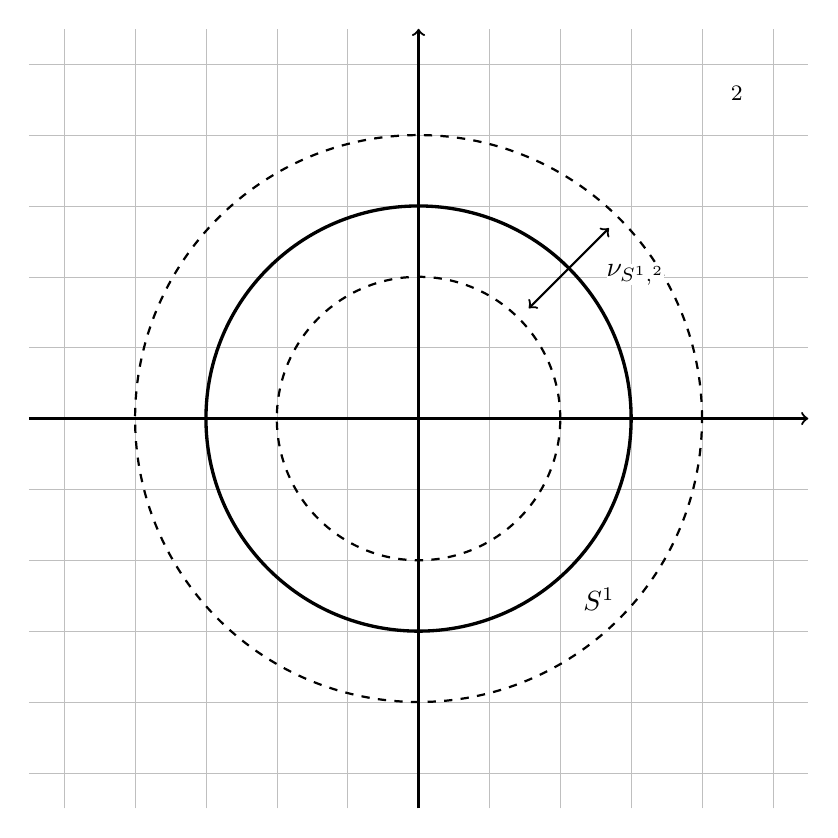
\begin{tikzpicture}[scale = .9, thick, every node/.style = {fill = white}]
		\draw[very thin, lightgray] (-5.5, -5.5) grid (5.5, 5.5);

		\draw[->] (-5.5, 0) -- (5.5, 0);
		\draw[->] (0, -5.5) -- (0, 5.5);

		\node[font = \large] at (4.5, 4.5) {$\R^2$};

		\draw[very thick] (0, 0) circle[radius = 3cm];
		\draw[dashed] 
			(0, 0) circle[radius = 2cm] 
			(0, 0) circle[radius = 4cm];

		\begin{scope}[rotate = -45]
			\draw[->] (0, 3) -- (0, 3.8);
			\draw[->] (0, 3) -- (0, 2.2);
			\node[inner sep = 0pt] at (.73, 3.6) {$\nu_{S^1, \R^2}$};
		\end{scope}


		\node[inner sep = 0pt] at (-45:3.6cm) {$S^1$};
	\end{tikzpicture}
	\caption{The tubular neighborhood from example \ref{ex:tubbynbdhsn} illustrated in the case $n = 1$.}
\end{figure}
\begin{theorem}[Tubular neighborhood theorem]\index{tubular neighborhood theorem}\label{thm:tubbynbhds}
	Every compact\footnote{(from me) This theorem holds more generally even for non-compact manifolds, cf. \cite[Theorem 6.24]{lee_introduction_2012}.} manifold $M \subseteq \R^n$ admits a tubular neighborhood.
\end{theorem}
\begin{proof}[Sketch of proof]
	As in example \ref{ex:tubbynbdhsn}, we define a map
	\begin{align*}
		f_\lambda\colon E(\nu_{M, \R^n}) &\to \R^n \\
		(x, v) &\mapsto x + \frac{v}{\lambda(1 + \lVert v\rVert)}
	\end{align*}
	The implicit function theorem implies that each $f_\lambda$ is an immersion on an open neighborhood of $M \subseteq E(\nu_{M, \R^n})$.
	The fact that $f_\lambda|_M = \id_M$ and compactness of $M$ then imply that for $\lambda \gg 0$ the map $f|_\lambda$ is an embedding.
\end{proof}
We now view $S^n = \R^n \cup \{\infty\}$ as pointed with basepoint $\infty$, and for a euclidean bundle $\xi\colon E \to B$ we equip $\Th(\xi) = D(\xi) / S(\xi)$ with the basepoint $[S(\xi)]$, the collapsed boundary of the disk bundle.

Let $M \subseteq \R^n$ be a closed $k$-dimensional submanifold with tubular neighborhood as constructed in the proof of theorem \ref{thm:tubbynbhds}.
Then we can define a continuous, pointed map
\begin{equation*}
	\Phi_M\colon S^n \to \Th(\gamma_\R^{n - k})
\end{equation*}
via the composite
\begin{equation*}
	\begin{tikzcd}[row sep = large]
		S^n 
				\ar[r, two heads]
			& S^n \big/ f\big(\mathring{D}(\nu_{M, \R^n})\big)^{\mathrm{C}}
			& f\big(D(\nu_{M, \R^n})\big) \big / f\big(S(\nu_{M, \R^n})\big)
				\ar[l, swap, "\isom"]
				\ar[from = 2-1, rounded corners, to path = {[pos = 1.1]
					-- ([xshift = -2ex] \tikztostart.west)
					|- ($(\tikzcdmatrixname-1-2)!0.5!(\tikzcdmatrixname-2-2)$) \tikztonodes
					-| ([xshift = 1em] \tikztotarget.east)
					-- (\tikztotarget)
				}, "f", "\isom"']
		\\
			\Th(\nu_{M, \R^n})
				\ar[r, "\Th(g)"]
			& \Th(\gamma_\R^{n - k, n})
				\ar[r, "(\RP^n \incl \RP^\infty)_*"]
			& \Th(\gamma_\R^{n - k})
	\end{tikzcd}
\end{equation*}
where $g\colon N_{M, \R^n} \to E(\gamma_\R^{n - k, n})$ is the Gauss map of the normal bundle of $M$.
\begin{proposition}\label{prop:pontryaginthom}
	\leavevmode
	\begin{enumerate}
		\item If $M, M' \subseteq \R^m$ are cobordant, then $\Phi_M$ is based-homotopic to $\Phi_{M'}$.
		\item Let $n > 1$ and $M_1, M_2 \subseteq \R^n$ be two closed manifolds.
			Assume that $M_1 \subseteq \mathring{D}_1$, $M_2 \subseteq \mathring{D}_2$ with $D_1 \cap D_2 = \emptyset$ two disjoint closed disks.
			Then $\Phi_{M_1 \sqcup M_2}$ represents the sum of $[\Phi_{M_1}]$ and $[\Phi_{M_2}]$ in $\pi_n(\Th(\gamma_\R^{n - k}))$.
	\end{enumerate}
\end{proposition}
\begin{corollary}
	The map
	\begin{align*}
		\Phi\colon \Bord_k^{(n)} &\to \pi_n(\Th(\gamma_\R^{n - k})) \\
		[M] &\mapsto [\Phi_M]
	\end{align*}
	is a group homomorphism.
\end{corollary}
\begin{proof}[Proof of proposition \ref{prop:pontryaginthom}]
	Let $N \subseteq \R^n \times [0, 1]$ be a cobordism from $M$ to $M'$.
	We can extend $N$ slightly to include $M \times \{0\}$ and $M' \times \{1\}$ in its interior by adding on $M \times (-\delta, 0]$ and $M' \times [1, 1 + \delta)$ for some small $\delta > 0$.
	We can then consider the tubular neighborhood $f^{\mathring{N}}$ of $\mathring{N}$.
	By construction, the normal space at each $x \in M$ equals $(N_{M, \R^n})_x \times \{0\}$ and likewise for $x \in M'$.
	% TODO picture
	Moreover, $f^{\mathring{N}}$ agrees with $f^M$ and $f^{M'}$, the tubular neighborhoods of $M$ and $M'$, respectively.
	Hence the composite
	\begin{equation*}
		\begin{tikzcd}[row sep = large]
			S^n \times [0, 1]
					\ar[r, two heads]
				& S^n \times [0, 1] \big / f^{\mathring{N}}\big(\mathring{D}(\nu_{N, \R^n \times \R})\big)^{\mathrm{C}}
				& \Th(\nu_{N, \R^n \times \R})
					\ar[l, swap, "\isom"]
					\ar[dll, rounded corners, to path = {[pos = 1]
						-- ([xshift = 1em] \tikztostart.east)
						|- ($(\tikzcdmatrixname-1-2)!0.5!(\tikzcdmatrixname-2-2)$) \tikztonodes
						-| ([xshift = -2ex] \tikztotarget.west)
						-- (\tikztotarget)
					}, swap, "\Th(g)"]
			\\
			\Th(\gamma_\R^{n - k, n + 1})
					\ar[r, "(\RP^{n + 1} \incl \RP^\infty)_*"]
				& \Th(\gamma_\R^{n - k})
		\end{tikzcd}
	\end{equation*}
	where $g$ is the Gauss map is a homotopy from $\Phi_M$ to $\Phi_{M'}$.

	For the second part, choose tubular neighborhoods $f^{M_1}$, $f^{M_2}$ of $M_1$ and $M_2$ (respectively) small enough such that $\img\big(f^{M_i}\big) \subseteq \mathring{D}_i$ ($i = 1, 2$).
	Then $f^{M_1} \sqcup f^{M_2} = f^{M_1 \sqcup M_2}$ is a tubular neighborhood for $M_1 \sqcup M_2$ and
	\begin{equation*}
		S^n \big/ f^{M_1 \sqcup M_2}\big(\mathring{D}(\nu_{M_1 \sqcup M_2, \R^n})\big)^{\mathrm{C}}
	\end{equation*}
	decomposes as 
	\begin{equation*}
		S^n \big/ f^{M_1}\big(\mathring{D}(\nu_{M_1, \R^n})\big)^{\mathrm{C}} \vee S^n \big/ f^{M_2}\big(\mathring{D}(\nu_{M_2, \R^n})\big)^{\mathrm{C}}
	\end{equation*}
	so that the projection $S^n \to S^n \big/ f^{M_1 \sqcup M_2}\big(\mathring{D}(\nu_{M_1 \sqcup M_2, \R^n})\big)^{\mathrm{C}}$ is the pinch sum of the respective projections for $M_1$ and $M_2$.
	The claim follows.
	% TODO picture
\end{proof}
\begin{theorem}[Thom \cite{thom_quelques_1954}]	
	The map $\Phi\colon \Bord_k^{(n)} \to \pi_n(\Th(\gamma_\R^{n - k}))$ is an isomorphism.
\end{theorem}
\begin{proof}
	We first aim to show surjectivity.
	For this, note that we can get back $M$ from $\Phi_M$ by taking the preimage of the zero-section in $\Th(\gamma_\R^{n - k})$.
	We now argue that for a general based map $g\colon S^n \to \Th(\gamma_\R^{n - k})$ we can always replace $g$ by a map $\tilde{g}$ homotopic to it such that the preimage of the zero-section under $\tilde{g}$ is a $k$-dimensional closed manifold in $\R^n \subseteq S^n$.
	This relies on a number of results from differential topology:
	\begin{proposition}
		\leavevmode
		\begin{enumerate}
			\item Every continuous map $\alpha\colon M \to N$ between manifolds can be approximated arbitrarily closely by a smooth one which is homotopic to it.
				If $\alpha$ is already smooth on a closed submanifold of $M$, the homotopy can be chosen to be constant on that submanifold.
			\item Given a smooth map $\alpha\colon M \to N$ between manifolds and a submanifold $N' \subseteq N$ such that $\dim M + \dim N' \geq N$, then there exists an arbitrarily close smooth function $\tilde{\alpha}$ homotopic to $\alpha$ which is \strong{transverse}\index{transversality} to $N'$.
				This means that if $n \in N'$ is a point and $m \in M$ such that $\tilde{\alpha}(m) = n$, then $\Tang_n N' + D \tilde{\alpha}_m (\Tang_m M) = \Tang_n N$.
			\item If $\alpha\colon M \to N$ is smooth and transverse to $N' \subseteq N$, then $\alpha^{-1}(N') \subseteq M$ is a smooth submanifold of dimension $\dim N' + \dim M - \dim N$.
		\end{enumerate}
	\end{proposition}
\end{proof}


\section{Exercises}
This section contains all of the weekly exercises and solutions for the course.
The solutions presented here are my own, unless explicitly stated otherwise.
Most of them have been checked by a pair of skilled eyes but by no means all, so tread with appropriate care.

At the end of the section (page \pageref{sect:quickquest} and following) you will find both sets of quick questions together with their (justified, again by me) answers.

\begin{exercise}\label{ex:serrefib}
	The goal of the first problem is to recall the notion of a Serre fibration and its homotopical properties.
	\begin{itemize}
		\item A map of spaces $p\colon E \to B$ has the \emph{homotopy lifting property with respect to a space $X$} if for every commutative diagram of the form
			\begin{equation*}
				\begin{tikzcd}
					X \times \{0\} 
							\ar[r, "\tilde{f}_0"]
							\ar[d, hook]
						& E
							\ar[d, "p"]
					\\
					X \times I
							\ar[r, "f"]
						& B
				\end{tikzcd}
			\end{equation*}
			there exists a map $\tilde{f}\colon X \times I \to E$ making the diagram commute.
		\item A map $p\colon E \to B$ has the \emph{homotopy lifting property with respect to a pair of spaces $(X, A)$} if for every commutative diagram of the form
			\begin{equation*}
				\begin{tikzcd}
					X \cup_A (A \times I)
							\ar[r]
							\ar[d, hook]
						& E
							\ar[d, "p"]
					\\
					X \times I
							\ar[r, "f"]
						& B
				\end{tikzcd}
			\end{equation*}
			there exists a map $\tilde{f}\colon X \times I \to E$ making the diagram commute. (The space $X \cup_A (A \times I)$ is defined by gluing $A \times I$ to $X$ along the natural map $A \times \{0\} \to X$.)
		\item A map of spaces $p\colon E \to B$ is said to be a \emph{Serre fibration} if it has the homotopy lifting property with respect to all discs $D^n$, $n \geq 0$.
			It can be shown that having the homotopy lifting property with respect to all discs is equivalent to having the homotopy lifting property with respect to all CW-pairs.
	\end{itemize}
	Furthermore, we recall the notion of a \emph{homotopy fibre}.
	For a space $X$ and $x \in X$ we let $P_x X$ denote the space of paths in $X$ to $x$, that is $P_x X \coloneq \{\gamma\colon I \to X \mid \gamma(1) = x\}$, equipped with the compact-open topology.
	Given a map $f\colon Y \to X$, the \emph{homotopy fibre} of $f$ at $x$ is then defined as the space
	\begin{equation*}
		\hofib_x(f) \coloneq P_x X \times_X Y = \{(y, \gamma) \in P_x \times Y \mid \gamma(0) = f(y)\}
	\end{equation*}
	Now let $p\colon E \to B$ be a Serre fibration and $b \in B$ a basepoint.
	We write $F = p^{-1}(b) \subseteq E$ for the fibre and define a map $\varphi\colon F \to \hofib_b(p)$ by the formula  
	\begin{equation*}
		z \mapsto (c(b), i(z))
	\end{equation*}
	Here, $c(b)$ denotes the constant path in $B$ at the basepoint $b$.

	Prove that $\varphi$ is a weak homotopy equivalence, i.e. that it induces an isomorphism on homotopy groups for all basepoints.
	\begin{hint}
		If you have trouble with the proof, first focus on showing that $\varphi$ induces a bijection on path components.
	\end{hint}
\end{exercise}

\begin{exercise}
	Let $C$ be a chain complex filtered by subcomplexes $C_0 \subseteq C_1 \subseteq C$.
	The pairs $(C_1, C_0)$ and $(C, C_1)$ have associated long exact sequences of homology groups
	\begin{equation}\label{ex2:les1}
		\cdots \to H_n(C_0) \to H_n(C_1) \xto{q_*} H_n(C_1 / C_0) \xto{\del^{(C_1, C_0)}} H_{n - 1}(C_0) \to \cdots
	\end{equation}
	and 
	\begin{equation}\label{ex2:les2}
		\cdots \to H_n(C_1) \to H_n(C) \to H_n(C / C_1) \xto{\del^{(C, C_1)}} H_{n - 1}(C_1) \to \cdots
	\end{equation}
	respectively.
	The goal of this exercise is to compute the homology of $C$ in terms of the homology of the complexes $C_0$, $C_1 / C_0$, and $C / C_1$.
	This is the length 2 special case of the spectral sequence associated to a filtered complex which we will later discuss in the lecture.
	\begin{enumerate}
		\item Use the long exact sequences above to define maps $f\colon H_*(C / C_1) \to H_{* - 1}(C_1 / C_0)$ and $g\colon H_*(C_1 / C_0) \to H_{* - 1}(C_0)$.
			Show that $g \circ f = 0$.
			In spectral sequence terminology, the maps $g$ and $f$ are the only potentially non-zero $d^1$-differentials.
		\item Next we will construct the only potentially nonzero $d^2$-differential.
			Use the long exact sequences above once more to construct another map $d\colon \ker(f) \to \coker(g)$ of degree $-1$ so that there are isomorphisms
			\begin{itemize}
				\item $\coker(d) \isom \img(H_*(C_0) \to H_*(C))$
				\item $\ker(g) / \img(f) \isom \img(H_*(C_1) \to H_*(C)) / \img(H_*(C_0) \to H_*(C))$
				\item $\ker(d) \isom H_*(C) / \img(H_*(C_1) \to H_*(C))$
			\end{itemize}
			where $\img({{-}})$ is the image of a map.
			In words, $\coker(d)$, $\ker(g) / \img(f)$, and $\ker(d)$ are isomorphic to the subquotients in the filtration on $H_*(C)$ given by the filtration on $H_*(C)$ given by the images of $H_*(C_0)$ and $H_*(C_1)$.
	\end{enumerate}
\end{exercise}
\begin{figure}[hb]
	\begin{equation*}
		\begin{tikzcd}[column sep = small]
			\cdots
					\ar[r, gray]
				& H_n(C_0)
					\ar[d, gray, "i^0_*"]
			\\
			\cdots
					\ar[r]
				& H_n(C_1)
					\ar[r, gray, "q^0_*"]
					\ar[d, "i^1_*"]
				& H_n(C_1 / C_0) 
					\ar[r, gray, "\del^0"]
					\ar[r, citecol, shift right = 1.5, swap, "g"]
				& H_{n - 1}(C_0)
					\ar[d, gray, "i^0_*"]
			\\
				& H_n(C)
					\ar[r, "q^1_*"]
				& H_n(C / C_1)
					\ar[r, "\del^1"]
					\ar[r, shift right = 1.5, highlightcol, dash]
				& H_{n - 1}(C_1)
					\ar[r, gray, "q_*^0"]
					\ar[r, shift right = 1.5, highlightcol, swap, "f" near start]
					\ar[d, "i_1^*"]
				& H_{n - 1}(C_1 / C_0)
					\ar[r, gray, "\del^0"]
				& \cdots
			\\
				& & & H_{n - 1}(C)
					\ar[r, "q^1_*"]
				& H_{n - 1}(C / C_1)
					\ar[r, "\del^1"]
				& \cdots
		\end{tikzcd}
	\end{equation*}
	\caption{%
		Sequences \ref{ex2:les1} and \ref{ex2:les2} arranged in a staircase diagram. 
		The morphisms belonging to sequence \ref{ex2:les1} are set in \textcolor{gray}{gray}.
		The two maps $f$ and $g$ constructed in part two of the exercise are highlight in \textcolor{highlightcol}{red} and \textcolor{citecol}{violet}, respectively.
	}
	\label{fig:staircase}
\end{figure}
\begin{solution}
	We will use the morphism names indicated in figure \ref{fig:staircase}.
	That figure will also be helpful for following along.
	\begin{enumerate}
		\item We put $f \coloneq q^0_* \circ \del^1$ and $g \coloneq \del^0$.
			Then $g \circ f = \del^0 \circ q^0_* \circ \del^1 = 0$ since $\del^0 \circ q^0_* = 0$ by exactness of sequence \ref{ex2:les1}.
		\item Note that the condition $g \circ f = 0$ amounts to saying that
			\begin{equation*}
				H_n(C / C_1) \xto{f} H_{n - 1}(C_1 / C_0) \xto{g} H_{n - 2}(C_0)
			\end{equation*}
			is a chain complex for all $n$; denoting its homology as $\bar{H}^0_n = \ker f$, $\bar{H}^1_{n - 1} = \ker g / \img f$, and $\bar{H}^2_{n - 2} = \coker g$, our goal is to find a map $d\colon \bar{H}^0_* \to \bar{H}^2_{* - 1}$ with the required properties.
			To this end, note that there is an isomorphism $\sigma\colon H_n(C_1) \supseteq \img i^0_* \isom \bar{H}^2_n$ since by exactness of sequence \ref{ex2:les1}, $\img g = \img \del^0 = \ker i^0_*$.
			We now put $d \coloneq \sigma \circ \del^1$.
			First of all, note that this composition is well-defined since if $\alpha \in \ker f$, then $q^0_*(\del^1(\alpha)) = 0$ implies that $\del^1(\alpha) \in \ker q^0_* = \img i^0_*$, so $\del^1(\alpha)$ is in the domain of $\sigma$.

			Now for the properties:
			\begin{itemize}
				\item Since $\img g = \ker i^0_*$ and $\img \del^1 = \ker i^1_*$ by exactness, we have $\coker d \isom (H_*(C_0) / \ker i^0_*) / \sigma(\ker i^1_*) \isom \img\bigg(H_*(C_0) \xto{i^1_* \circ i^0_*} H_*(C)\bigg)$ since $\sigma$ is the inverse to the quotient isomorphism $H_*(C_0) / \ker i^0_* \xto{\isom} \img i^0_*$. 
				\item For this item we will do a diagram chase.
					Our goal is to define a surjective map $\varphi\colon \ker g \to \img i^1_* / \img (i^1_* \circ i^0_*)$ whose kernel is $\img f$.
					In fact, let us put $\varphi(x) \coloneq [y]$ where $y \in \img i^1_* \subseteq H_n(C)$ is the image $i^1_*(y')$ of an element $y' \in (q^0_*)^{-1}(x) \subseteq H_n(C_1)$.
					This is well-defined: 
					First of all, we note that $\ker g = \ker \del^0 = \img q^0_*$ so that we can take preimages under $q^0_*$.
					Next, if $y'' \in (q^0_*)^{-1}(x)$ is another lift, we note that $q^0_*(y' - y'') = 0$, thus $y' - y'' \in \img i^0_*$ by exactness. 
					Therefore, $i^1_*(y' - y'') \in \img (i_1^* \circ i_0^*)$ which is to say that $[i_1^*(y')] = [i_1^*(y'')]$ in the quotient, i.e. the choice of lift $y'$ does not matter.

					For surjectivity, we note again that $\ker q^0_* = \img i^0_*$, which implies that $\varphi$ is surjective since the map $H_*(C_1) / \img i^0_* \to \img i^1_* / \img (i^1_* \circ i^0_*)$ induced by $i^1$ is and $\bar{q}^0_*\colon H_*(C_1) / \img i^0_* \to \img q^0_*$ is an isomorphism.

					Finally, we have on one hand that $\img f \subseteq \ker \varphi$ as $\img f = \img q^0_*|_{\img \del^1} = \img q^0_*|_{\ker i^1_*}$, i.e. $(q^0_*)^{-1}(z) \in \ker i^1_*$ for all $z \in \img f$ and therefore $\varphi(z) = 0$, while on the other $\ker \varphi \subseteq \img f$ as well:
					Saying that $\varphi(z) = 0$ for some $z \in \ker g$ is equivalent to saying that $i^1_*(z') \in \img (i^1_* \circ i^0_*)$ for any lift $z' \in (q^0_*)^{-1}(z)$ by definition.
					But $\ker q^0_* = \img i^0_*$, so fixing $0 \in H_*(C_1)$ as the lift of $0 \in \ker g$ without loss of generality, we may assume that $z' \in \ker i^1_* = \img \del^1$, in other words that there exists a preimage $z'' \in (\del^1)^{-1}(z)$ such that $f(z'') = z$, i.e. $z \in \img f$.
				\item Since $\sigma$ is an isomorphism, we see that 
					\begin{equation*}
						\ker d = \ker \del^1 = \img q^1_* \isom H_*(C) / \ker q^1_* = H_*(C) / \img i^1_* 
					\end{equation*}
					using the exactness of sequence \ref{ex2:les2}.
			\end{itemize}
			This concludes the proof.
			\qedhere
	\end{enumerate}
\end{solution}

\begin{exercise}\label{ex:gysinwang}
	\leavevmode
	\begin{enumerate}
		\item Suppose that $S^n \to E \to B$ is a fibre sequence, $n \neq 0$, $B$ simply connected.
			Show that there is a long exact sequence of the form
			\begin{equation*}
				\cdots \to H_{p - n}(B) \to H_p(E) \to H_p(B) \to H_{p - n - 1}(B) \to H_{p - 1}(E) \to \cdots
			\end{equation*}
			This sequence is called the \strong{Gysin sequence}\index{Gysin sequence} of the sphere bundle.
		\item Let $F \to E \to S^n$ be a fibre sequence over a sphere with $n \neq 0, 1$.
			Show that there exists a long exact sequence of the form
			\begin{equation*}
				\cdots \to H_q(F) \to H_q(E) \to H_{q - n}(F) \to H_{q - 1}(F) \to H_{q - 1}(E) \to \cdots
			\end{equation*}
			This sequence is called the \strong{Wang sequence}\index{Wang sequence}.
	\end{enumerate}
\end{exercise}
\begin{solution}
	\leavevmode
	\begin{enumerate}
		\item Consider the homological Serre spectral sequence for $S^n \to E \to B$ (which we can do since $S^n$ is connected and $B$ simply connected).
			On the $E^2$-page, we have that
			\begin{equation}\label{ex:gysinwang:gysingroups}
				E^2_{p, q} = H_p(B; H_q(S^n)) \isom \begin{cases}
					H_p(B) 	& q = 0, n \\
					0 		& \text{else}
				\end{cases}
			\end{equation}
			since $H_q(S^n) \isom \Z$ if $q = 0, n$ and 0 else.
			Therefore, the only possible non-trivial differentials are $d^{n + 1}\colon E^{n + 1}_{p, 0} \to E^{n + 1}_{p - n - 1, n}$ for any $p$.
			Turning to the $E^\infty$-page, we see that every antidiagonal passes through at most two non-trivial groups, namely 
			\begin{equation*}
				E^\infty_{p, n} \isom \coker\big(d^{n + 1}\colon E^{n + 1}_{p + n + 1, 0} \to E^{n + 1}_{p, n}\big)
			\end{equation*}
			and 
			\begin{equation*}
				E^\infty_{p - n, 0} \isom \ker\big(d^{n + 1}\colon E^{n + 1}_{p - n, 0} \to E^{n + 1}_{p - 2n - 1, n}\big)
			\end{equation*}
			Thus, we have short exact sequences
			\begin{equation}\label{ex:gysinwang:inftyseq}
				0 \to E^\infty_{p, n} \xto{\iota} H_p(E) \xto{\pi} E^\infty_{p - n, 0} \to 0
			\end{equation}
			for all $p$.
			Putting all of this together, we obtain a long exact sequence
			\begin{equation*}
				\begin{tikzcd}[column sep = small]
					\cdots 
							\ar[r]
						& E^{n + 1}_{p, 0}
							\ar[r, "d^{n + 1}"]
						&[1em] E^{n + 1}_{p - n - 1, n}
							\ar[r, "\iota \circ \coker(d^{n + 1})"]
						&[4em] H_{p - 1}(E)
							\ar[r, "\kappa \circ \pi"]
						&[1em] E^{n + 1}_{p - 1, 0} 
							\ar[r]
						& \cdots
				\end{tikzcd}
			\end{equation*}
			where $\kappa\colon E^\infty_{p - 1, 0} \incl E^{n + 1}_{p - 1, 0}$ is the kernel inclusion of the outgoing differential (this is exact since $\coker(d^{n + 1})$ is surjective and $\kappa$ is injective, by which exactness at and around $H_{p - 1}(E)$ reduces to exactness of sequence \eqref{ex:gysinwang:inftyseq}).
			Finally substituting in the groups from equation \eqref{ex:gysinwang:gysingroups} for the $E^{n + 1}$-terms yields the claim.
		\item This part is almost entirely analogous to part one so we will allow ourselves to be somewhat brief.

			Note that the $E^2$-page of the associated homological Serre spectral sequence of the given fibre sequence has the form
			\begin{equation}\label{ex:gysinwang:wanggroups}
				E^2_{p, q} = H_p(S^n; H_q(F)) \isom \begin{cases}
					H_q(F)  & p = 0, n \\
					0 		& \text{else}
				\end{cases}
			\end{equation}
			so that all nontrivial differentials are of the form $d^n\colon E^n_{n, q} \to E^n_{0, q + n - 1}$ for $q$ any.
			On the $E^\infty$-page, we again have a maximum of two nonzero entries per antidiagonal leading to short exact sequences
			\begin{equation*}
				0 \to E^\infty_{0, q} \to H_q(E) \to E^\infty_{n, q - n} \to 0
			\end{equation*}
			for any $q$.
			In this situation we can identify $E^\infty_{0, q}$ and $E^\infty_{n, q - n}$ with the cokernel and kernel of the in- and outgoing differentials, respectively, like before so we obtain a long exact sequence
			\begin{equation*}
				\begin{tikzcd}
					\cdots 
							\ar[r]
						& E^n_{0, q}
							\ar[r]
						& H_q(E)
							\ar[r]
						& E^n_{n, q - n}
							\ar[r, "d^n"]
						& E^n_{0, q - 1}
							\ar[r]
						& \cdots
				\end{tikzcd}
			\end{equation*}
			which yields the Wang sequence after plugging in the groups from equation \eqref{ex:gysinwang:wanggroups}.
			\qedhere
	\end{enumerate}
\end{solution}

\begin{exercise}
	Let $X$ be a simply connected space which is not weakly contractible.
	Prove that it is not possible for both $X$ and $\Omega X$ to have the homotopy type of a finite CW-complex.
	\begin{hint}
		\leavevmode
		\begin{enumerate}
			\item Use the Hurewicz theorem to find a prime $p$ such that both $\tilde{H}_*(X; \F_p)$ and $\tilde{H}_*(\Omega X; \F_p)$ are nontrivial.
			\item Consider the fibre sequence $\Omega X \to * \to X$.
		\end{enumerate}
	\end{hint}
\end{exercise}
\begin{solution}
	Let us start out by proving the following algebraic lemma:
	\begin{lemma}
		Let $A \neq 0$ be a $\Z$-module.
		Then there exists some prime $p \in \Z \cup \{\infty\}$ such that $A \tensor_{\Z} \F_p \neq 0$.
		Here we define $\F_\infty \coloneq \Q$.
	\end{lemma}
	\begin{smallproof}
		As $A \tensor_{\Z} \Q \isom A / \tors(A)$ where $\tors(A) \coloneq \{a \in A \mid na = 0 \text{ for some } n \in \Z\}$ we can choose $p = \infty$ whenever $A$ is not entirely torsion.
		Otherwise, pick a prime $p$ such that $A$ has $p$-torsion.
		We then note that the map $A \xto{\cdot p} A$ is not surjective: if it were, we would have $A / \ker p \isom A$, but $A / \ker p$ does not have any $p$-torsion while $A$ does.
		Therefore, $A \tensor_{\Z} \F_p \isom A / p A$ is non-trivial.
	\end{smallproof}
	Let now $n > 1$ be minimal such that $\pi_n X \neq 0$ (such an $n$ exists since $X$ is not weakly contractible and simply connected).
	Since $\pi_k \Omega X \isom \pi_{k + 1} X$ for all $k$, this implies that $\pi_{n - 1} \Omega X \isom \pi_n X$ is the first non-trivial homotopy group of $\Omega X$ as well, so noting that in the case $n = 2$ the group $\pi_1 \Omega X \isom \pi_2 X$ is already abelian\footnote{so that $(\pi_1 \Omega X)^\text{ab} = \pi_1 \Omega X$ for the $n = 1$ special case of the Hurewicz theorem}, the Hurewicz theorem yields isomorphisms $H_n(X) \isom H_{n - 1}(\Omega X) \isom \pi_n X \neq 0$.

	An application of the universal coefficient theorem now tells us that
	\begin{equation*}
		H_n(X; \F_p) \isom (H_n(X; \Z) \tensor \F_p) \dsum \Tor(\underbrace{H_{n - 1}(X; \Z)}_{= 0}, \F_p) \isom H_n(X; \Z) \tensor_{\Z} \F_p
	\end{equation*}
	so by the lemma there is a prime $p$ with $H_n(X; \F_p) \neq 0$ and $H_{n - 1}(\Omega X; \F_p) \neq 0$. Applying the universal coefficient theorem once more, this time over the field $\F_p$, we see that 
	\begin{equation*}
		H_n(X; H_m(\Omega X; \F_p)) \isom H_n(X; \F_p) \tensor_{\F_p} H_m(\Omega X; \F_p)
	\end{equation*}
	The tensor product on the right hand side here is zero if and only if both $H_n(X; \F_p)$ and $H_m(\Omega X; \F_p)$ are since they are vector spaces and therefore free.

	This has the consequence that if $H_*(X; \Z)$ and $H_*(\Omega X; \Z)$ are both concentrated in degrees $0, \ldots, k$ and $0, \ldots, l$ respectively for some $k, l \in \N$, then so are the groups $H_*(X; H_*(\Omega X; \F_p))$ (with the appropriate bigrading), and if we take $k$ and $l$ to be tight then $H_k(X; H_l(\Omega X; \F_p)) \neq 0$.
	Looking now at the homological Serre spectral sequence for the fibre sequence $\Omega X \to * \to X$, this translates to $E^2_{k, l}$ being non-zero.
	But since $E^2_{n, m} = 0$ whenever $n > k$ or $m > l$, no incoming our outgoing differential at this group is ever non-trivial and it survives onto the $E^\infty$-page.
	But the total space is a point, so the $E^\infty$-page is a barren wasteland save for $E^\infty_{0, 0} \isom \F_p$, which is a contradiction!
	Thus the $\F_p$-homology of at least one of $X$ or $\Omega X$ must be infinite, whence we conclude that space cannot be (weakly) homotopy equivalent to a finite CW-complex since the homology of a finite CW-complex is again finite (via cellular homology).
\end{solution}

\begin{exercise}
	The $E_\infty$-term of the Serre spectral sequence will not determine the cohomology of the total space uniquely in general because of extension problems.
	Give an example of two fibre sequences $F \to Y \to X$ with $F = \RP^\infty$ and $X = \CP^\infty$ such that the $E_r$-pages of both Serre spectral sequences are isomorphic for all $r$, but $H^\bullet(E; \Z) \neq H^\bullet(E'; \Z)$.
	\begin{hint}
		Show that there are exactly two homotopy classes of maps $\CP^\infty \to K(\Zn{2}, 2)$ and consider their homotopy fibres.
	\end{hint}
\end{exercise}
\begin{solution}
	By the representability of ordinary cohomology, there is a natural bijection $[\CP^\infty, K(\Zn{2}, 2)]_* \isom H^2(\CP^\infty; \Zn{2}) \isom \Zn{2}$.
	Thus, exactly two homotopy classes of maps $\CP^\infty \to K(\Zn{2}, 2)$ exist; let $f$ represent the trivial and $g$ the non-trivial class and let $F_f$ and $F_g$ be their respective homotopy fibres.
	We then obtain long exact sequences
	\begin{equation*}
		\begin{tikzcd}
			0
					\ar[r]
				& \pi_2 F_f
					\ar[r]
				& \underbrace{\pi_2 \CP^\infty}_{\isom \Z}
					\ar[r, "f_*", "= 0"']
				& \underbrace{\pi_2 K(\Zn{2}, 2)}_{\isom \Zn{2}}
					\ar[r]
				& \pi_1 F_f
					\ar[r]
				& 0
		\end{tikzcd}
	\end{equation*}
	and
	\begin{equation*}
		\begin{tikzcd}
			0
					\ar[r]
				& \pi_2 F_g
					\ar[r]
				& \underbrace{\pi_2 \CP^\infty}_{\isom \Z}
					\ar[r, two heads, "g_*"]
				& \underbrace{\pi_2 K(\Zn{2}, 2)}_{\isom \Zn{2}}
					\ar[r]
				& \pi_1 F_g
					\ar[r]
				& 0
		\end{tikzcd}
	\end{equation*}
	using that $\CP^\infty$ is a $K(\Z, 2)$ to see that all remaining terms in the sequences are zero.
	By choice, we have that $f_* = 0$ and that $g_*$ realizes the quotient projection $\Z \twoheadrightarrow \Zn{2}$, so we can read off that
	\begin{equation*}
		\pi_k F_f \isom \begin{cases}
			\Z 		& k = 2 \\
			\Zn{2} 	& k = 1 \\
			0 		& \text{else}
		\end{cases}
	\end{equation*}
	and
	\begin{equation*}
		\pi_k F_g \isom \begin{cases}
			\Z 		& k = 2 \\
			0 		& \text{else}
		\end{cases}
	\end{equation*}
	In particular, this implies that $H_1(F_f) \isom \Zn{2}$ and therefore that $H^2(F_f)$ has 2-torsion whereas $H_1(F_g) = 0$ and $H_2(F_g) \isom \Z$ implies that $H^2(F_g) \isom \Z$ as well (all via Hurewicz and the universal coefficient theorem), so $H^*(F_f) \mathrel{\not\isom} H^*(F_g)$.
	However, taking another round of homotopy fibres we obtain fibre sequences
	\begin{gather*}
		\RP^\infty \to F_f \to \CP^\infty \\
		\RP^\infty \to F_g \to \CP^\infty 
	\end{gather*}
	using that $\Omega K(\Zn{2}, 2)$ is a $K(\Zn{2}, 1)$ and that all (CW-models of) $K(\Zn{2}, 1)$ are homotopy equivalent.
	Considering the (cohomological) Serre spectral sequence(s) associated to these two fibre sequences, we start out with $E_2^{p, q} = H^p(\CP^\infty; H^q(\RP^\infty)) \isom H^p(\CP^\infty) \tensor_{\Z} H^q(\RP^\infty)$ as $H^*(\CP^\infty)$ is free and of finite type, so $E_2^{p, q} \neq 0$ if and only if $p$ and $q$ are both even (as $H^*(\CP^\infty) \isom \Z[x]$ and $H^*(\RP^\infty) \isom \Z[y] / (2y)$ with $|x| = |y| = 2$).
	But any differential $d^r$ is a map of bidegree $(r, 1 - r)$, and as only one of $r$ and $1 - r$ is ever even at the same time, no nontrivial differentials exist and the $E_2$-page is in fact the $E_\infty$-page (in particular, no information about $F_f$ or $F_g$ influences these data via the differentials).
\end{solution}

\begin{exercise}
	Use the Serre spectral sequence to compute $H^*(F; \Z)$ for $F$ the homotopy fibre of a map $S^k \to S^k$ of degree $n$ for $k, n > 1$ and show that the cup product structure on $H^*(F; \Z)$ is trivial.
\end{exercise}
\begin{solution}
	Let $f\colon S^k \to S^k$ be a map of degree $n$ (i.e. $f_*\colon H_k(S_k) \to H_k(S_k)$ is multiplication by $n$).
	We will start out by gathering some information.
	First off, note that the induced map $f_*\colon \pi_k S^k \to \pi_k S^k$ is also multiplication by $n$:
	This follows from the naturality of the Hurewicz isomorphism and the fact that $S^k$ is $(k - 1)$-connected.
	We thus get a long exact sequence 
	\begin{equation*}
		\begin{tikzcd}
			\cdots 
					\ar[r]
				&\pi_{k + 1} S^k
					\ar[r]
				&\pi_k F 
					\ar[r]
				&\underbrace{\pi_k S^k}_{\isom \Z}
					\ar[r, "f_*", "= (\cdot n)"']
				&\underbrace{\pi_k S^k}_{\isom \Z}
					\ar[r]
				&\pi_{k - 1} F 
					\ar[r]
				& 0
		\end{tikzcd}
	\end{equation*}
	with the zero at the right coming from the group $\pi_{k - 1} S^k = 0$.
	As such, we have an isomorphism $\pi_{k - 1} F \isom \coker f_* \isom \coker(\Z \xto{\cdot n} \Z) = \Zn{n}$.
	As below degree $k - 1$ the long exact sequence collapses, $\pi_{k - 1} F$ is in fact the lowest non-trivial homotopy group of $F$; accordingly, Hurewicz tells us that $H_{n - 1}(F) \isom \pi_{k - 1} F \isom \Zn{n}$ is the lowest non-trivial homology group of $F$ (noting for the case $k = 2$ that $\Zn{n}$ is abelian).

	We will now move on to considering the Serre spectral sequence(s) for the fibre sequence $F \to S^k \xto{f} S^k$.
	Although our goal is to also determine the cohomology \emph{ring}, we will start out by calculating $H_*(F)$ using the homological version of the Serre spectral sequence because it avoids an extension problem on the $k$th antidiagonal arising in cohomology.
	Since the homology of $S^k$ is free and finite, we have isomorphisms
	\begin{equation*}
		E^2_{p, q} = H_p(S^k; H_q(F)) \isom H_p(S^k) \tensor H_q(F)
	\end{equation*}
	so $E^2_{p, q} = 0$ if $p \neq 0, k$ or $0 \neq q < k - 1$.
	In particular, the only possibly non-trivial differentials are $d^k\colon E^k_{k, q} \to E^k_{0, q + k - 1}$ for any $q$, so in particular the differential
	\begin{equation*}
		d^k\colon \underbrace{E^k_{k, 0}}_{\isom \Z} \to \underbrace{E^k_{0, k - 1}}_{\isom \Zn{n}}
	\end{equation*}
	must be surjective as the $(k - 1)$st antidiagonal on the $E_\infty$-page must be trivial since $H_{k - 1}(S^k) = 0$.
	Moving upwards, all antidiagonals become zero, and therefore all differentials isomorphisms, so using that $E^k_{k, q} \isom E^k_{0, q}$, we find by induction that 
	\begin{equation*}
		H_m(F) \isom \begin{cases}
			\Z 		& m = 0 \\
			\Zn{n} 	& (k - 1) \mid m \text{ and } m > 0 \\
			0 		& \text{else}
		\end{cases}
	\end{equation*}
	With help of the universal coefficient theorem, we deduce that
	\begin{equation*}
		H^m(F) \isom \begin{cases}
			\Z 		& m = 0 \\
			\Zn{n} 	& (k - 1) \mid (m - 1) \text{ and } m > 1 \\
			0 		& \text{else}
		\end{cases}
	\end{equation*}
	The distribution of nontrivial degrees in $H^*(F)$ is almost enough to conclude triviality of the cup product structure:
	If $k > 2$, then given $\alpha, \beta \in H^*(F)$ of degree $|\alpha| = a (k - 1) + 1$ and $|\beta| = b (k - 1) + 1$, respectively, we have $|\alpha \beta| = |\alpha| + |\beta| = (a + b)(k - 1) + 2$ which is not of the form $c(k - 1) + 1$ for any $c \in \N$ and therefore the product $\alpha \beta$ \enquote{falls through the grates.} 
	For $n = 2$, however, there are no grates to fall through as $H^m(F) \isom \Zn{n}$ for all $m \geq 2$, so we resort to studying the \emph{cohomological} Serre spectral sequence:
	Similar to before, we have an isomorphism
	\begin{equation*}
		E_2^{\bullet, \bullet} \isom H^\bullet(S^2) \tensor_{\Z} H^\bullet(F) \isom \Lambda(e) \tensor_{\Z} H^\bullet(F)
	\end{equation*}
	of bigraded rings for $e \in H^2(S^2)$ a generator since $H^*(S^2)$ is nice.
	The differential
	\begin{equation*}
		d_2\colon \underbrace{E_2^{0, 2}}_{\isom \Zn{n}} \to \underbrace{E_2^{2, 1}}_{= 0}
	\end{equation*}
	starting at the first interesting group in the $p = 0$ column is necessarily trivial, its codomain being 0.
	Above that, all differentials
	\begin{equation*}
		d_2\colon \underbrace{E_2^{0, q}}_{\isom \Zn{n}} \to \underbrace{E_2^{2, q - 1}}_{\isom \Zn{n}}
	\end{equation*}
	are isomorphisms for convergence reasons.
	Let $x_i \in H^i(F)$ be a generator for all $i \geq 2$, and let $x_1 \in H^1(F) = 0$ denote a \enquote{ghost class}\footnote{a fancy name for 0 :)}.
	Then $E^2_{2, q - 1}$ is generated by $e x_{q - i}$ for all $q \geq 2$, and we may without loss of generality arrange that $d_2(x_i) = e x_{i - 1}$ whenever $i \geq 2$ (noting the special case $d_2(x_2) = e x_1 = 0$).
	Let now $i$ be minimal with the property that $l x_i = x_{i - a} x_a$ for some $l \in \Zn{n}$, $2 \leq a \leq i - 2$.
	Using that differentials are graded derivations, we compute
	\begin{align*}
		l e x_{i - 1} = d_2(l x_i) &= d_2(x_{i - a} x_a) \\
								   &= d_2(x_{i - a}) \cdot x_a + (-1)^{i - a} x_{i - a} \cdot d_2(x_a) \\
								   &= e x_{i - a - 1} \cdot x_a + (-1)^{i - a} x_{i - a} \cdot e x_{a - 1} \\
								   &= e (x_{i - a - 1} \cdot x_a + (-1)^{i - a} x_{i - a} \cdot x_{a - 1})
	\end{align*}
	(noting that this makes sense with our convention for $x_1$).
	But $l e x_{i - 1} \neq 0$, so at least one of $x_{i - a - 1} x_a$ or $x_{i - a} x_{a - 1}$ is nonzero as well and therefore a multiple of the generator $x_{i - 1} \in H^{i - 1}(F)$, contradicting minimality of $i$.
	We thus conclude that $x_i x_j = 0$ for all $i, j$ and therefore that the ring structure on $H^*(F)$ is trivial.
\end{solution}

\begin{exercise}
	Use the Serre spectral sequence to compute $\pi_5(S^3, *)$.
	\begin{hint}
		\leavevmode
		\begin{enumerate}
			\item Use the Whitehead tower for $S^3$.
			\item There are different ways to go about this, but you might need to know $H_n(K(\Zn{2}, 3))$ for $n \leq 5$.
				For this, recall that
				\begin{equation*}
					H_n(K(\Zn{2}, 1)) \isom \begin{cases}
						\Z 		& n = 0 \\
						\Zn{2} 	& n \text{ odd} \\
						0 		& n \text{ even and } n > 0 \\
					\end{cases}
				\end{equation*}
				Start with the path-loop fibration of $K(\Zn{2}, 2)$ to compute $H_n(K(\Zn{2}, 2))$ in low degrees, then do the same for $K(\Zn{2}, 3)$.
		\end{enumerate}
	\end{hint}
\end{exercise}
\begin{solution}
	\emph{For following along, it might be helpful to consider the $E_2$-pages of the spectral sequences used in this argument printed on page \pageref{fig:firstspecseq}, although one should be careful that these include all the computed results already.}

	Let 
	\begin{equation*}
		\begin{tikzcd}
			\cdots
				\ar[d]
			\\
			\tau_{\geq 5} S^3
				\ar[d, "\phi_5"]
			\\
			\tau_{\geq 4} S^3
				\ar[d, "\phi_4"]
			\\
			S^3
		\end{tikzcd}
	\end{equation*}
	be a Whitehead tower for $S^3$\footnote{We adopt the convention that $\tau_{\geq n} X$ is $(n - 1)$-connected with $\pi_k(\tau_{\geq n} X, *) \isom \pi_k(X, *)$ for all $k \geq n$.}.
	Exploiting the usual Hurewicz trick, it is enough to compute $H_5(\tau_{\geq 5} S^3) \isom \pi_5(\tau_{\geq 5} S^3, *) \isom \pi_5(S^3, *)$.
	Noting that we already know that $\pi_4(\tau_{\geq 4} S^3, *) \isom \pi_4(S^3, *) \isom \Zn{2}$ from the lecture, we have two Serre fibrations
	\begin{gather*}
		K(\Zn{2}, 3) \to \tau_{\geq 5} S^3 \xto{\phi_5} \tau_{\geq 4} S^3 \mathrlap{\quad\text{and}}\\
		K(\Z, 2) \to \tau_{\geq 4} S^3 \xto{\phi_4} S^3
	\end{gather*}
	The second fibration should look familiar, and recalling the uniqueness theorem for Whitehead towers (or one particular method of their construction with which this coincides) we see that we have already calculated $H^*(\tau_{\geq 4} S^3)$ in example 2.31 in the lecture\footnote{Actually, the indices in the in-lecture calculation are incorrect (if I have noted them down correctly), but this is easily remedied by having a good look at it.} to be  
	\begin{equation*}
		H_n(\tau_{\geq 4} S^3) \isom \begin{cases}
			\Z 		& n = 0 \\
			\Zn{k} 	& n = 2k \text{ and } k > 1 \\
			0 		& \text{else}
		\end{cases}
	\end{equation*}
	With this input, we can attempt a calculation:
	Consider the Serre spectral sequence for $K(\Zn{2}, 3) \to \tau_{\geq 5} S^3 \to \tau_{\geq 4} S^3$ with $E_2$-page
	\begin{equation*}
		E^2_{p, q} = H_p(\tau_{\geq 4} S^3; H^q(K(\Zn{2}, 3)))
	\end{equation*}
	The lowest index at which a non-zero term appears is $E^2_{0, 3} \isom \Zn{2}$, with only interesting differential $d^4\colon \Zn{2} \isom E^4_{4, 0} \to E^4_{0, 3} \isom \Zn{2}$, which must be an isomorphism as $\tau_{\geq 5} S^3$ is 4-connected (via Hurewicz).
	Next, we note that $E^2_{0, 4} \isom H_4(K(\Zn{2}, 3)) = 0$ since it has no incoming interesting differentials and converges to 0.
	Moreover, we note that the only unknown group on the 5th antidiagonal of the convergence is $E^\infty_{0, 5}$, and that there is only one incoming interesting differential at that index, namely $d^6\colon \Zn{3} \isom E^6_{6, 0} \to E^6_{0, 5}$.
	This differential is trivial (either by noting that $H_*(K(\Zn{2}, 3))$ is 2-power-torsion via Serre class theory or by the direct calculation of $H_5(K(\Zn{2}, 3))$ which we are about to undertake), so we obtain that 
	\begin{equation*}
		\pi_5(\tau_{\geq 5} S^3, *) \isom H_5(\tau_{\geq 5} S^3) \isom E^\infty_{0, 5} \isom E^2_{0, 5} \isom H_5(K(\Zn{2}, 3))
	\end{equation*}
	Let us thus calculate this latter group.
	Our present spectral sequence will take us no further in this effort, so we make use of the usual trick of iteratively computing (co)homology of $K(G, n)$s via path-loop fibrations.
	We start out with $(\Omega K(\Zn{2}, 2) \to P K(\Zn{2}, 2) \to K(\Zn{2}, 2)) \htpyeqv (\RP^\infty \to * \to K(\Zn{2}, 2))$ and consider the Serre spectral sequence with $E_2$-page
	\begin{equation*}
		E_2^{*, *} = H^*(K(\Zn{2}, 2); H^*(\RP^\infty))
	\end{equation*}
	The first interesting trivial differential (between the first nonzero groups) is $d_3\colon \Zn{2} \isom E_3^{0, 2} \to E_3^{3, 0} \isom \Zn{2}$ which we see must be an isomorphism, being the only differential affecting either group and seeing as the total space is contractible.
	In multiplicative terms, if we let $x \in H^2(\RP^\infty)$ be the generator and $e \in H^3(K(\Zn{2}, 3))$ the unique nontrivial class, this is equivalent to $d_3(x) = e$.
	Staying in the same column(s), the next interesting differential is $d_3\colon \Zn{2} \isom E_3^{0, 4} \to E_3^{3, 2} \isom \Zn{2}$.
	Multiplicatively, this is given by the formula $d_3(x^2) = d_3(x) x + x d_3(x) = 2 x d_3(x) = 0$ and therefore trivial.
	We now look further to the right.
	The group $E_2^{4, 0}$ is trivial as it has no potentially nontrivial incoming differentials, all nontrivial groups left of it sitting in even rows.
	Looking now at the group $E_2^{5, 0}$, we find exactly two potential incoming differentials: One from $E_5^{0, 4}$ (which we have previously found to survive its outoing $d_3$ and which is unaffected by any $d_4$s for degree reasons) and one from $E_3^{2, 2} \isom E_2^{2, 2}$.
	One may at first glance be surprised that this latter group is non-zero, but via the universal coefficient theorem we compute $E_2^{2, 2} \isom H^2(K(\Zn{2}, 2); \Zn{2}) \isom \Hom(H_2(K(\Zn{2}, 2)), \Zn{2}) \dsum \Ext(H_1(K(\Zn{2}, 2)), \Zn{2}) \isom \Zn{2}$ as $H_2(K(\Zn{2}, 2)) \isom \Zn{2}$ and $H_1(K(\Zn{2}, 2)) = 0$.
	Accordingly, we find that $E_2^{5, 0} \eqcolon A$ is some mystery group of order 4, being given by the extension problem
	\begin{equation*}
		\begin{tikzcd}
			0 
					\ar[r]
				& \underbrace{\Zn{2}}_{\isom E_3^{2, 2}}
					\ar[r, hook]
				& A
					\ar[r, two heads]
				& \underbrace{\Zn{2}}_{\isom E_5^{0, 4}}
					\ar[r]
				& 0
		\end{tikzcd}	
	\end{equation*}
	as these differentials present the last chances for the involved groups to die.
	We will content ourselves with not determining $A$ further and move on.

	Next, consider the Serre spectral sequence of the fibre sequence $K(\Zn{2}, 2) \to * \to K(\Zn{2}, 3)$ with $E_2$-page
	\begin{equation*}
		E^2_{*, *} = H_*(K(\Zn{2}, 3); H_*(\Zn{2}, 2))
	\end{equation*}
	Noting that we have computed (via a standard application of the universal coefficient theorem) that
	\begin{equation*}
		H_k(K(\Zn{2}, 2)) \isom \begin{cases}
			\Z & k = 0 \\
			\Zn{2} & k = 2 \\
			A & k = 4 \\
			0 & k < 5 \text{ odd}
		\end{cases}
	\end{equation*}
	and that we know
	\begin{equation*}
		H_k(K(\Zn{2}, 3)) \isom \begin{cases}
			\Z & k = 0 \\
			\Zn{2} & k = 3 \\
			0 & k \neq 0, 3 \text{ and } k \leq 4
		\end{cases}
	\end{equation*}
	we quickly see that the of all the outgoing differentials of $E^2_{5, 0}$, the only interesting one is $d^5\colon E^5_{5, 0} \to E^5_{0, 4} \isom A$ as all other differentials have trivial codomain.
	The only other incoming differential to $E^5_{0, 4}$ is $d_3^{3, 2}\colon \Zn{2} \isom E_3^{3, 2} \to E^3_{0, 4}$ and these together must kill it, so in particular we see that $E^5_{0, 4} \neq 0$ as $\coker d_3^{3, 2}$ is a group of order at least two. Unfortunately, distinguishing between the cases $E^5_{5, 0} \isom A$ and $E^5_{5, 0} \isom \Zn{2}$ seems intractable here, so we resort to yet another spectral sequence.

	Observe that from any short exact sequence $0 \to G \to F \to H \to 0$ of abelian groups, we can obtain fibre sequences $K(G, n) \to K(F, n) \to K(H, n)$ for all $n \geq 1$ by realizing the second map as a map $\pi_n(K(F, n)) \to \pi_n(K(H, n))$\footnote{This can be done (in the case $n > 1$ which is the only case interesting us here) e.g. via direct construction by building up $K(F, n)$ and $K(H, n)$ starting with a wedge sum of copies of $S^n$ for each generator of the respective group, realizing the map on these generators, attaching $(n + 1)$-cells to realize all necessary relations between these generators, and finally killing all higher homotopy groups. It is part of the proof that this construction works that the map so constructed can be extended over all higher cells.}, taking the homotopy fibre and noting that the long exact sequence of homotopy groups implies that it is a $K(G, n)$.
	We apply this to 
	\begin{equation*}
		0 \to \Z \to \Z \to \Zn{2} \to 0
	\end{equation*}
	with $n = 3$ to obtain a fibre sequence $K(\Z, 3) \to K(\Z, 3) \to K(\Zn{2}, 3)$.
	Unfortunately, we do not have a good understanding of the (co)homology of $K(\Z, 3)$ right now, so we will have to make yet another detour through the path-loop fibration and study the fibre sequence $\CP^\infty \htpyeqv K(\Z, 2) \to * \to K(\Z, 3)$.
	Consider therefore the Serre spectral sequence with $E_2$-page
	\begin{equation*}
		E_2^{*, *} = H^*(K(\Z, 3); H^*(\CP^\infty)) \isom H^*(K(\Z, 3)) \tensor H^*(\CP^\infty) \isom H^*(K(\Z, 3)) \tensor \Z[x]
	\end{equation*}
	using that $H^*(\CP^\infty)$ is free and of finite type for the first and that $H^*(\CP^\infty) \isom \Z[x]$ with $x \in H^2(\CP^\infty)$ a generator for the second isomorphism.
	By Hurewicz and universal coefficients, the first nonzero reduced cohomology group of $K(\Z, 3)$ is $H^3(K(\Z, 3)) \isom \Z$.
	In particular, it seems wise to start the calculation by considering all differentials of the form $d_3\colon \Z \isom E_3^{0, 2q} \to E_3^{3, 2(q - 1)} \isom \Z$.
	The first such differential, $d_3^{0, 2}$ must be an isomorphism, presenting the only chance both for domain and codomain to die.
	In other words, $d_3(x) = e$ where $e \in E^3_{3, 0} \isom H^3(K(\Z, 3))$ is a generator.
	Two places up, we then have $d_3(x^2) = d_3(x) x + x d_3(x) = 2 e x$, i.e. $d_3^{0, 4}$ is multiplication by 2.
	Let us move to the right now.
	Clearly $E_2^{4, 0} = E_2^{5, 0} = 0$ as all differentials ending in these groups begin in a trivial group, so we turn to $E_2^{6, 0}$.
	Here we only have a single potential ingoing differential, namely $d_3^{3, 2}$.
	At $E_3^{3, 2}$ we therefore get both an incoming $d_3$, which is multiplication by 2, and an outgoing $d_3$, whose kernel must therefore contain $2\Z$ and which must kill both domain and codomain.
	The only way to make this work is if $E_3^{6, 0} \isom E_2^{6, 0} \isom \Zn{2}$.

	We now return to our penultimate sequence, for which we have now gathered enough information to proceed.
	We consider the Serre spectral sequence with $E_2$-page
	\begin{equation*}
		E_2^{*, *} \isom H^*(K(\Zn{2}, 3); H^*(K(\Z, 3)))
	\end{equation*}
	Keeping in mind that our goal is to calculate $H^6(K(\Zn{2}, 3)) \isom H_5(K(\Zn{2}, 3))$, we find ourselves lucky:
	There is \emph{no} incoming differential at $E_2^{6, 0}$, all other relevant nontrivial groups living at $(0, 0)$, $(0, 3)$, $(4, 0)$, $(4, 3)$, and $(0, 6)$.
	In other words, $E_2^{6, 0} \isom E_\infty^{6, 0}$ and therefore $E_2^{6, 0}$ contributes to the convergence to $H^6(K(\Z, 3)) \isom \Zn{2}$, so since $\Zn{2}$ does not admit any interesting filtrations we directly conclude that $E_2^{6, 0} = 0$ or $E_2^{6, 0} \isom \Zn{2}$.
	But the first case we have excluded earlier, so we finally conclude that $\Zn{2} \isom H^6(K(\Zn{2}, 3)) \isom H_5(K(\Zn{2}, 3)) \isom \pi_5(S^3, *)$.
\end{solution}

\begin{exercise}
	Compute the cohomology of the space $\map(S^1, S^3)$ of continuous (not necessarily basepoint-preserving) maps $f\colon S^1 \to S^3$.
\end{exercise}
\begin{solution}
	There is a Serre fibration $\Omega S^3 \xto{\iota} \map(S^1, S^3) \xto{\ev_1} S^3$ as $S^1$ is locally compact and well-pointed.
	Consider first the long exact sequence of homotopy groups associated to this fibration, which ends in
	\begin{equation*}
		\begin{tikzcd}[column sep = 2.6em]
			\cdots 
					\ar[r]
				& \pi_3(\map(S^1, S^3), *)
					\ar[r, "(\ev_1)_*"]
				& \pi_3(S^3, *)
					\ar[dll, rounded corners, swap, to path = {[pos = 1]
						-- ([xshift = 1em] \tikztostart.east)
						|- ($(\tikzcdmatrixname-1-2)!0.5!(\tikzcdmatrixname-2-2)$) \tikztonodes
						-| ([xshift = -2ex] \tikztotarget.west)
						-- (\tikztotarget)
					}]
			\\ 
			\pi_2(\Omega S^3, *)
					\ar[r, "\iota_*"]
				& \pi_2(\map(S^1, S^3), *)
					\ar[r]
				& 0
		\end{tikzcd}
	\end{equation*}
	as $S^3$ is 2-connected and $\Omega S^3$ simply connected.
	Note that $\ev_1\colon \map(S^1, S^3) \to S^3$ admits a section, namely $\sigma\colon S^3 \to \map(S^1, S^3)$ being given by $\sigma(x) = \const_x$, the constant loop at $x$.
	This implies that $(\ev_1)_*\colon \pi_*(\map(S^1, S^3), *) \to \pi_*(S^3, *)$ is surjective, so we can deduce that $\iota_*\colon \pi_2(\Omega S^3, *) \to \pi_2(\map(S^1, S^3), *)$ is an isomorphism, i.e. $\pi_2(\map(S^1, S^3), *) \to \pi_2(\Omega S^3, *) \isom \pi_3(S^3, *) \isom \Z$.
	By Hurewicz, this further implies that $H_2(\map(S^1, S^3)) \isom \Z$ and therefore $H^2(\map(S^1, S^3)) \isom \Z$ by the universal coefficient theorem.

	We now consider the Serre spectral sequence with $E_2$-page
	\begin{equation*}
		E_2^{*, *} = H^*(S^3; H^*(\Omega S^3)) \isom H^*(S^3) \tensor H^*(\Omega S^3) \isom \Lambda(e) \tensor \Gamma(x)
	\end{equation*}
	where $e \in H^3(S^3)$ and $x \in H^2(\Omega S^3)$ generators, with the first isomorphism stemming from the fact that $H^*(S^3)$ is free and finite and the second from the description of these rings calculated in the lecture.
	For the differentials, the only possibly nonzero candidates are all of the form $d_3\colon E_3^{0, q} \to E_3^{3, q - 2}$ with $q$ even and $\geq 2$.
	But note that the first such differential, $d_3^{0, 2}\colon \Z \isom E_3^{0, 2} \to E_3^{3, 0} \isom \Z$ must be trivial: Certainly $\ker d_3^{0, 2} \isom \Z$ as it is the only group contributing to the convergence to $H^2(\map(S^1, S^3)) \isom \Z$, so $d_3^{0, 2}$ must be multiplication by some $k > 1$; but then its cokernel is torsion and isomorphic to $H^3(\map(S^1, S^3))$ (as it is lonely remaining on the third antidiagonal) which is torsion-free via the universal coefficient theorem as by our calculation of $H_2(\map(S^1, S^3)) \isom \Z$ above.

	Long story short, $d_3^{0, 2}$ is trivial, and reexpressed in multiplicative terms we see that $d_3(x) = 0$.
	But every other $E_3^{0, 2q}$-group is generated by divided powers of $x$, so all other differentials must be trivial as well (as $0 = d^3(x^k) = d^3\big(k! \cdot \frac{x^k}{k!}\big)$ implies that $d^3\big(\frac{x^k}{k!}\big) = 0$ by freeness).
	In other words, $E_\infty^{*, *} \isom E_2^{*, *}$ as bigraded rings, so since no antigiagonal contains more than one nontrivial term, we obtain that $H^*(\map(S^1, S^3)) \isom \Lambda(e) \tensor \Gamma(x)$ with $e \in H^3(\map(S^1, S^3))$ and $x \in H^2(\map(S^1, S^3))$ generators.
\end{solution}
\begin{figure}[p!]
	\centering
	\tikzsetnextfilename{excs_postnikov5_specseq}
	\begin{tikzpicture}[
		pagemember/.style = {
			fill = white, 
			font = \scriptsize, 
			inner sep = 0.5pt
		},
		differential/.style = {
			commutative diagrams/every arrow, 
			thick, 
			preaction = {
				draw = white, 
				arrows = -, 
				line width = 0.5ex
			}
		}]
		\matrix[
			name = m, 
			nodes in empty cells, 
			matrix of math nodes, 
			nodes = {outer sep = 0ex, inner sep = 2pt},
			column sep = {4.5ex, between origins},
			%row sep = {4ex, between origins},
			row sep = 0.5ex,
			column 1/.style = {anchor = base east, font = \scriptsize}, 
			row 8/.style = {font = \scriptsize}] {
				5 &[-2ex] \Zn{2} & 0 & 0 & 0 	  & \Zn{2} & \Zn{2}	& ? 	 \\
				4 & 0  			 & 0 & 0 & 0 	  & 0 	   & 0 		& 0  	 \\
				3 & \Zn{2}		 & 0 & 0 & 0      & \Zn{2} & \Zn{2}	& ? 	 \\
				2 & 0  			 & 0 & 0 & 0 	  & 0  	   & 0 		& 0 	 \\
				1 & 0  			 & 0 & 0 & 0 	  & 0  	   & 0 		& 0 	 \\
				0 & \Z 			 & 0 & 0 & 0 	  & \Zn{2} & 0 		& \Zn{3} \\
			 	  & 0  			 & 1 & 2 & 3 	  & 4      & 5  	& 6 	 \\
		};

		% bounding box coordinates for the "graph" drawing area
		\coordinate (top left) at ($(m-1-2.north west) + (0, 0.3)$);
		\coordinate (bottom left) at (m-6-2.south west -| top left);
		\coordinate (bottom right) at ($(bottom left -| m-6-8.south east) + (0.3, 0)$);
		\coordinate (top right) at (bottom right |- top left);

		\draw[spectral sequence/axis, line cap = round] (bottom left) -- (bottom right) node[below] {$p$};
		\draw[spectral sequence/axis, line cap = round] (bottom left) -- (top left) node[left] {$q$};

		\node[font = \scriptsize, draw, anchor = west] at (top right) {$E^2_{p, q} = H_p(\tau_{\geq 4} S^3; H_q(K(\Zn{2}, 3)))$};
\end{tikzpicture}
	\caption{$E^2$-page of the Serre spectral sequence for $K(\Zn{2}, 3) \to \tau_{\geq 5} S^3 \to \tau_{\geq 4} S^3$}
	\label{fig:firstspecseq}
\end{figure}
\begin{figure}[p!]
	\centering
	\tikzsetnextfilename{excs_rpinfty_specseq}
	\begin{tikzpicture}[
		pagemember/.style = {
			fill = white, 
			font = \scriptsize, 
			inner sep = 0.5pt
		},
		differential/.style = {
			commutative diagrams/every arrow, 
			thick, 
			preaction = {
				draw = white, 
				arrows = -, 
				line width = 0.5ex
			}
		}]
		\matrix[
			name = m, 
			nodes in empty cells, 
			matrix of math nodes, 
			nodes = {outer sep = 0ex, inner sep = 2pt},
			column sep = {4.5ex, between origins},
			%row sep = {4ex, between origins},
			row sep = 0.5ex,
			column 1/.style = {anchor = base east, font = \scriptsize}, 
			row 6/.style = {font = \scriptsize}] {
				4 &[-2ex] \Zn{2} & 0 & \Zn{2} & \Zn{2} 	  & ? 	   & ? 		  	 \\
				3 & 0			 & 0 & 0 & 0 & 0 & 	0 			 \\
				2 & \Zn{2}		 & 0 & \Zn{2} & \Zn{2} 	  & ?  	   & ? 		 	 \\
				1 & 0  			 & 0 & 0 & 0 	  & 0  	   & 0 		 	 \\
				0 & \Z 			 & 0 & 0 & \Zn{2} & 0 	   & A 		  \\
			 	  & 0  			 & 1 & 2 & 3 	  & 4      & 5  	 	 \\
		};

		% bounding box coordinates for the "graph" drawing area
		\coordinate (top left) at ($(m-1-2.north west) + (0, 0.3)$);
		\coordinate (bottom left) at (m-5-2.south west -| top left);
		\coordinate (bottom right) at ($(bottom left -| m-5-7.south east) + (0.3, 0)$);
		\coordinate (top right) at (bottom right |- top left);

		\draw[spectral sequence/axis, line cap = round] (bottom left) -- (bottom right) node[below] {$p$};
		\draw[spectral sequence/axis, line cap = round] (bottom left) -- (top left) node[left] {$q$};

		\node[font = \scriptsize, draw, anchor = west] at (top right) {$E_2^{p, q} = H^p(K(\Zn{2}, 2); H^q(\RP^\infty))$};
\end{tikzpicture}
	\caption{$E^2$-page of the Serre spectral sequence for $\RP^\infty \to * \to K(\Zn{2}, 2)$}
\end{figure}
\begin{figure}[p!]
	\centering
	\tikzsetnextfilename{excs_K_Zn2_2_K_Zn2_3_specseq}
	\begin{tikzpicture}[
		pagemember/.style = {
			fill = white, 
			font = \scriptsize, 
			inner sep = 0.5pt
		},
		differential/.style = {
			commutative diagrams/every arrow, 
			thick, 
			preaction = {
				draw = white, 
				arrows = -, 
				line width = 0.5ex
			}
		}]
		\matrix[
			name = m, 
			nodes in empty cells, 
			matrix of math nodes, 
			nodes = {outer sep = 0ex, inner sep = 2pt},
			column sep = {4.5ex, between origins},
			row sep = 0.5ex,
			column 1/.style = {anchor = base east, font = \scriptsize}, 
			row 6/.style = {font = \scriptsize}] {
				4 &[-2ex] A 	 & 0 & 0 & ? 	  & ? 	   & ? 		  	 \\
				3 & 0			 & 0 & 0 & 0 & 0 & 	0 			 \\
				2 & \Zn{2}		 & 0 & 0 & \Zn{2} 	  & \Zn{2}  	   & \Zn{2} 		 	 \\
				1 & 0  			 & 0 & 0 & 0 	  & 0  	   & 0 		 	 \\
				0 & \Z 			 & 0 & 0 & \Zn{2} & 0 	   & \Zn{2} 		  \\
			 	  & 0  			 & 1 & 2 & 3 	  & 4      & 5  	 	 \\
		};

		% bounding box coordinates for the "graph" drawing area
		\coordinate (top left) at ($(m-1-2.north west -| m-3-2.west) + (0, 0.3)$);
		\coordinate (bottom left) at (m-5-2.south west -| top left);
		\coordinate (bottom right) at ($(bottom left -| m-5-7.south east) + (0.3, 0)$);
		\coordinate (top right) at (bottom right |- top left);

		\draw[spectral sequence/axis, line cap = round] (bottom left) -- (bottom right) node[below] {$p$};
		\draw[spectral sequence/axis, line cap = round] (bottom left) -- (top left) node[left] {$q$};

		\node[font = \scriptsize, draw, anchor = west] at (top right) {$E^2_{p, q} = H_p(K(\Zn{2}, 3); H_q(K(\Zn{2}, 2)))$};
\end{tikzpicture}
	\caption{$E^2$-page of the Serre spectral sequence for $K(\Zn{2}, 2) \to * \to K(\Zn{2}, 3)$}
\end{figure}
\begin{figure}[p!]
	\centering
	\tikzsetnextfilename{excs_cpinfty_specseq}
	\begin{tikzpicture}[
		pagemember/.style = {
			fill = white, 
			font = \scriptsize, 
			inner sep = 0.5pt
		},
		differential/.style = {
			commutative diagrams/every arrow, 
			thick, 
			preaction = {
				draw = white, 
				arrows = -, 
				line width = 0.5ex
			}
		}]
		\matrix[
			name = m, 
			nodes in empty cells, 
			matrix of math nodes, 
			nodes = {outer sep = 0ex, inner sep = 2pt},
			column sep = {4ex, between origins},
			%row sep = {4ex, between origins},
			row sep = 0.5ex,
			column 1/.style = {anchor = base east, font = \scriptsize}, 
			row 6/.style = {font = \scriptsize}] {
				4 &[-2ex] \Z & 0 & 0 & \Z & 0 & 0 & \Zn{2} \\
				3 & 0  		 & 0 & 0 & 0  & 0 & 0 & 0 	   \\
				2 & \Z 		 & 0 & 0 & \Z & 0 & 0 & \Zn{2} \\
				1 & 0  		 & 0 & 0 & 0  & 0 & 0 & 0 	   \\
				0 & \Z 		 & 0 & 0 & \Z & 0 & 0 & \Zn{2} \\
			 	  & 0 & 1 & 2 & 3 & 4 & 5 & 6 \\
		};

		% bounding box coordinates for the "graph" drawing area
		\coordinate (bottom left) at (m-5-2.south west);
		\coordinate (bottom right) at ($(bottom left -| m-5-8.south east) + (0.3, 0)$);
		\coordinate (top left) at ($(m-1-2.north west) + (0, 0.3)$);
		\coordinate (top right) at (bottom right |- top left);

		\draw[spectral sequence/axis, line cap = round] (bottom left) -- (bottom right) node[below] {$p$};
		\draw[spectral sequence/axis, line cap = round] (bottom left) -- (top left) node[left] {$q$};

		\node[font = \scriptsize, draw, anchor = west] at (top right) {$E_2^{p, q} = H^p(K(\Z, 3)) \tensor H^q(\CP^\infty)$};
\end{tikzpicture}
	\caption{$E_2$-page of the Serre spectral sequence for $\CP^\infty \to * \to K(\Z, 3)$}
\end{figure}
\begin{figure}[p!]
	\centering
	\tikzsetnextfilename{excs_K_Z_3_K_Zn2_3_specseq}
	\begin{tikzpicture}[
		pagemember/.style = {
			fill = white, 
			font = \scriptsize, 
			inner sep = 0.5pt
		},
		differential/.style = {
			commutative diagrams/every arrow, 
			thick, 
			preaction = {
				draw = white, 
				arrows = -, 
				line width = 0.5ex
			}
		}]
		\matrix[
			name = m, 
			nodes in empty cells, 
			matrix of math nodes, 
			nodes = {outer sep = 0ex, inner sep = 2pt},
			column sep = {4.5ex, between origins},
			%row sep = {4ex, between origins},
			row sep = 0.5ex,
			column 1/.style = {anchor = base east, font = \scriptsize}, 
			row 8/.style = {font = \scriptsize}] {
				6 &[-1.5ex] \Zn{2} & 0 & 0 & \Zn{2} & \Zn{2} & \Zn{2} & \Zn{2} \\
				5 & 0  			 & 0 & 0 & 0 	  & 0 	   & 0 	 	& 0 	 \\
				4 & 0  			 & 0 & 0 & 0 	  & 0 	   & 0 		& 0  	 \\
				3 & \Z 			 & 0 & 0 & 0 	  & \Zn{2} & 0 		& \Zn{2} \\
				2 & 0  			 & 0 & 0 & 0 	  & 0  	   & 0 		& 0 	 \\
				1 & 0  			 & 0 & 0 & 0 	  & 0  	   & 0 		& 0 	 \\
				0 & \Z 			 & 0 & 0 & 0 	  & \Zn{2} & 0 		& \Zn{2} \\
			 	  & 0  			 & 1 & 2 & 3 	  & 4      & 5  	& 6 	 \\
		};

		% bounding box coordinates for the "graph" drawing area
		\coordinate (top left) at ($(m-1-2.north west) + (0, 0.3)$);
		\coordinate (bottom left) at (m-7-2.south west -| top left);
		\coordinate (bottom right) at ($(bottom left -| m-7-8.south east) + (0.3, 0)$);
		\coordinate (top right) at (bottom right |- top left);

		\draw[spectral sequence/axis, line cap = round] (bottom left) -- (bottom right) node[below] {$p$};
		\draw[spectral sequence/axis, line cap = round] (bottom left) -- (top left) node[left] {$q$};

		\node[font = \scriptsize, draw, anchor = west] at (top right) {$E_2^{p, q} = H^p(K(\Zn{2}, 3); H^q(K(\Z, 3)))$};
\end{tikzpicture}
	\caption{$E_2$-page of the Serre spectral sequence for $K(\Z, 3) \to K(\Z, 3) \to K(\Zn{2}, 3)$}
\end{figure}

\begin{exercise}
	\leavevmode
	\begin{enumerate}
		\item Consider the fibre sequence
			\begin{equation*}
				S^0 \to S^1 \xto{p} S^1
			\end{equation*}
			where $p\colon S^1 \to S^1$ denotes the 2-sheeted cover $p(z) = z^2$.
			Let $H_0(F_{({{-}})}, \Z)$ denote the local coefficient system on $S^1$ induced by the fibration.

			Show that local coefficient homology $H_*(S^1, H_0(F_{({{-}})}; \Z))$ is not isomorphic to the homology $H_*(S^1, H_0(S^1; \Z))$ with the constant coefficient system $H_0(S; \Z)$.
		\item Let $X$ be a connected CW-complex with basepoint $x \in X$ and universal cover $q\colon \tilde{X} \to X$.
			We suppose that $\pi_1(X, x)$ acts on another CW-complex $Y$.
			This also induces an action on homology,
			\begin{equation*}
				\alpha\colon \pi_1(X, x) \times H_*(Y; \Z) \to H_*(Y; \Z)
			\end{equation*}
			Now consider the fibre bundle
			\begin{equation*}
				Y \to \tilde{X} \times_{\pi_1(X, x)} Y \xto{q \times x} X
			\end{equation*}
			with $\pi_1(X, x)$ acting on $\tilde{X}$ through deck transformations and $\tilde{X} \times_{\pi_1(X, x)} Y$ is defined as the quotient of $\tilde{X} \times Y$ by the diagonal $\pi_1(X, x)$-action. 
			(You do not have to show that this is a fibre bundle.)

			As described in the lecture, the homologies of the fibres form a functor on the fundamental groupoid of $X$.
			In particular, the fundamental group $\pi_1(X, x)$ acts on the homology of the fibre at the point $x$, which canonically identifies with $Y$.
			Let $\beta\colon \pi_1(X, x) \times H_*(Y; \Z) \to H_*(Y; \Z)$ denote this action.

			Show that the two actions $\alpha$ and $\beta$ on homology are the same.
	\end{enumerate}
\end{exercise}

\begin{exercise}
	Prove the following, making use of the Serre spectral sequence:
	\begin{theorem}[Leray-Hirsch]
		Let $F \xto{i} E \xto{p} B$ be a fibration, with $B$ path-connected.
		Assume that there exists a set of classes $\{c_j\} \in H^*(E; \Z)$, of which only finitely many lie in a given degree, such that their restrictions $\{i^*(c_j)\}$ form a $\Z$-basis for the cohomology $H^*(F; \Z)$ of the fibre $F$.
		Then the set $\{c_j\}$ is a basis of $H^*(E; \Z)$ as a module over the ring $H^*(B; \Z)$.
	\end{theorem}
\end{exercise}
\begin{solution}
	We will start out by proving a lemma:
	\begin{lemma}
		Let $F \xto{i} E \xto{p} B$ be fibration with $B$ path-connected such that $i^*\colon H^*(E) \to H^*(F)$ is surjective.
		Then:
		\begin{enumerate}
			\item The action of $\pi_1(B, *)$ on $H^*(F)$ is trivial.
			\item All differentials of the form $d_n^{0, q}\colon E_n^{0, q} \to E_n^{n, q - n + 1}$ for $n, q \geq 0$ in the associated cohomological Serre spectral sequence are trivial.
		\end{enumerate}
	\end{lemma}
	\begin{smallproof}
		Let us consider the Serre spectral sequence for the given fibration with $E_2$-term
		\begin{equation*}
			E_2^{p, q} = H^p(B; H^q(F_{-}; \Z))
		\end{equation*}
		We then have edge homomorphisms $e(p)\colon H^q(E) \to E_\infty^{0, q} \incl E_2^{0, q} \isom H^0(B; H^q(F_{-})) \to H^q(F_*)$ for $* \in E$ any basepoint which agrees with the surjective map $i^*\colon H^q(E) \to H^*(F)$.
		In particular, this means that $H^0(B; H^q(F_{-})) \to H^q(F_*)$ must be surjective, so the action of $\pi_1(B, *)$ on $H^*(F)$ must be trivial\footnote{Life is hard (and short) enough so we will not prove this here, but it is not too difficult to see that $H^0(B; H^q(F_{-})) \isom H^q(F_*)$ is the \enquote{maximal} case that occurs when the $\pi_1(B, *)$-action is trivial, any element acting nontrivially killing some part of the left hand side by a calculation similar to what we did in exercise 1.1. (Apparently, if one is so inclined, one can show that $H^0(B; H^q(F_{-}))) \isom H^q(F)^{\pi_1(B, *)}$, the fixed points of $H^q(F)$ under the $\pi_1(B, *)$-action.)}.
		
		For the second statement, note that our spectral sequence now satisfies
		\begin{equation*}
			E_2^{p, q} \isom H^p(B; H^q(F; \Z))
		\end{equation*}
		as we have just shown the local coefficient system to be constant.
		In the leftmost column (of the first quadrant) we then recover $H^q(F) \isom E_2^{0, q}$.
		Accordingly, if any outgoing differential there is non-trivial, it kills some element of its domain (by not including it in its kernel), so we obtain that $E_\infty^{0, q} \subsetneq E_2^{0, q}$.
		But then $E_2^{0, q} \setminus E_\infty^{0, q}$ is not in the image of the edge homomorphism $e(p)\colon H^q(E) \to H^q(F)$ discussed above, contradicting its surjectivity; thus no such differential exists.
	\end{smallproof}

	Back in the problem setting, $i^*$ is surjective by assumption, so we are freed from working with local coefficients.
	Additionally, the assumption that $H^*(F)$ is free and of finite type gives rise to Serre spectral sequence with $E_2$-term
	\begin{equation*}
		E_2^{*, *} = H^*(B; H^*(F)) \isom H^*(B) \tensor H^*(F)
	\end{equation*}
	The second part of our lemma now tells us that all differentials originating on the $q$-axis are trivial, and this implies already that \emph{all} differentials are trivial:
	All groups on the $E_2$-page are generated by elements of the form $i^*(c_j) b_k$ with $b_k \in E_2^{p, 0} \isom H^p(B)$ for some $p, j, k \geq 0$, but
	\begin{equation*}
		d_2(i^*(c_j) b_k) = \underbrace{d_2(i^*(c_j))}_{= 0} b_k \pm i^*(c_j) \underbrace{d_2(b_k)}_{= 0} = 0
	\end{equation*}
	as the $i^*(c_j)$ live on the $q$- and the $b_k$ on the $p$-axis (where all outgoing differentials run off the page), so $E_3^{*, *} \isom E_2^{*, *}$ and inductively  by the same argument $E_\infty^{*, *} \isom E_2^{*, *}$.
	To finish the proof, we make use of lemma 2.28 from the lecture\footnote{\enquote{Given filtered graded abelian groups $(A, F), (B, G)$ such that the filtrations are in every degree eventually 0, any graded filtration-preserving morphism $f\colon A \to B$ that induces an isomorphism on all associated graded pieces is an isomorphism.}}.
	Consider the map $f\colon H^*(B) \tensor H^*(F) \to H^*(E)$ given by (linearly extending) $f(b \tensor i^*(c_j)) \coloneq p^*(b) \smile c_j$.
	This map preserves the natural grading on the domain and is compatible with the filtrations induced on domain and codomain from the $E_\infty$-page (in particular, filtering the domain by degree of the $H^*(F)$-factor).
	By our description of the $E_\infty$-page (in particular noting that it agrees with its multiplicative structure), it is an isomorphism on graded pieces, so we conclude that it is an isomorphism of graded abelian groups, which was to be shown.
\end{solution}

\begin{exercise}\label{ex:postnikovaction}
	Let $X$ be a connected CW-complex with basepoint $x \in X$.
	Recall that for each $n \geq 1$, $\pi_1(X, x)$ acts on $\pi_n(X, x)$.
	In the homotopy category, this induces a natural action of $\pi_1 X$ on $K(\pi_n(X, x), n)$ which further induces an action on homology
	\begin{equation*}
		\alpha\colon \pi_1(X, x) \times H_* K(\pi_n(X, x), n) \to H_* K(\pi_n(X, x), n)
	\end{equation*}
	Recall that for each $n \geq 2$, the Postnikov tower gives a fibre sequence
	\begin{equation*}
		K(\pi_n X, n) \to \tau_{\leq n} X \to \tau_{\leq n - 1} X
	\end{equation*}
	Let $f_{n - 1}\colon X \to \tau_{\leq n - 1} X$ be the canonical map and let $y = f_{n - 1}(x)$.
	Then $\pi_1(\tau_{\leq n - 1} X, y)$ acts on the homology of the homotopy fibre at the point $y$, i.e. $K(\pi_n(X, x), n)$.
	Let
	\begin{equation*}
		\beta\colon \pi_1(\tau_{\leq n - 1} X, y) \times H_* K(\pi_n(X, x), n) \to H_* K(\pi_n(X, x), n)
	\end{equation*}
	denote this action.
	Show that the two actions $\alpha$ and $\beta$ on homology are the same, under the identification
	\begin{equation*}
		(f_{n - 1})_*\colon \pi_1(X, x) \xto{\isom} \pi_1(\tau_{\leq n - 1} X, y)
	\end{equation*}
\end{exercise}

\begin{exercise}
	As discussed in the lecture, the first $p$-torsion class in $\pi_* S^3$ is found in degree $2p$.
	Recall that for all $n \geq 3$, the Hopf map $\eta\colon S^3 \to S^2$ induces an isomorphism $\eta_*\colon \pi_n S^3 \isom \pi_n S^2$.
	We let $x \in \pi_{2p} S^2$ be a $p$-torsion class.
	Consider the suspension $\Sigma x \in \pi_{2p + 1} S^3$.

	Show that if $p$ is odd, then $\Sigma x = 0$.

	Bonus: Show that when $p = 2$, $\Sigma x$ suspends to a generator of $\pi_5 S^3$.
\end{exercise}
\begin{solution}
	Consider the map $S^3 \to K(\Z, 3)$ inducing the identity on $\pi_3({{-}})$ and take its homotopy fibre to obtain a fibre sequence $F \to S^3 \to K(\Z, 3)$.
	We have seen the calculation of 
	\begin{equation*}
		H_n(F) \isom \begin{cases}
			\Zn{k} 	& n = 2k\; (k > 1) \\
			0 		& \text{else}
		\end{cases}
	\end{equation*}
	in the lecture.
	Using henceforth the letter $r$ in place of $p$ so as to avoid clashing with the usual notation for spectral sequences, we now look at the map $\rho\colon F \to K(\Zn{r}, 2r)$ inducing an isomorphism on the $r$-torsion part of $\pi_{2r}(F)$ (we have seen in the lecture that the $r$-torsion part of $\pi_{2r}(F) \isom \pi_{2r}(S^3)$ is isomorphic to $\Zn{r}$) and take another round of homotopy fibres to obtain a fibre sequence $F' \to F \to K(\Zn{r}, 2r)$.
	The only \enquote{interesting}\footnote{since in all lower and higher degrees $\pi_*(K(\Zn{r}, 2r))$ becomes 0 so that $\pi_k(F') \isom \pi_k(F)$} excerpt of the associated long exact sequence of homotopy groups reads
	\begin{equation*}
		\begin{tikzcd}
			0
					\ar[r]
				& \pi_{2r}(F')
					\ar[r]
				& \pi_{2r}(F)
					\ar[r, two heads]
				& \pi_{2r}(K(\Zn{r}, 2r))
				\ar[dll, rounded corners, to path = {[pos = 1]
					-- ([xshift = 1em] \tikztostart.east)
					|- ($(\tikzcdmatrixname-1-3)!0.5!(\tikzcdmatrixname-2-3)$) \tikztonodes
					-| ([xshift = -1em] \tikztotarget.west)
					-- (\tikztotarget)
				}, swap, "0"]
			\\
				& \pi_{2r - 1}(F')
					\ar[r]
				& \pi_{2r - 1}(F)
					\ar[r]
				& 0
		\end{tikzcd}
	\end{equation*}
	with the connecting map trivial since the preceding map is surjective by construction.
	In other words, we have
	\begin{equation*}
		\pi_k(F') \isom \begin{cases}
			\pi_k(F) / \ker \rho & k = 2r \\
			\pi_k(F) 			 & \text{else}
		\end{cases}
	\end{equation*}
	so in particular $\pi_k(F') \in \catfont{C}$ for all $k < 2r + 1$ where $\catfont{C}$ is the Serre class of finite abelian groups of order coprime to $r$.
	If we can show that $\pi_{2r + 1}(F') \isom \pi_{2r + 1}(F) \isom \pi_{2r + 1}(S^3) \in \catfont{C}$ we are obviously done, and by the modulo $\catfont{C}$ Hurewicz theorem this reduces to showing that $H_{2r + 1}(F') \in \catfont{C}$.
	We will now in fact show that $H_{2r + 1}(F') = 0 \in \catfont{C}$.

	Consider the Serre spectral sequence with $E^2$-page
	\begin{equation*}
		E^2_{p, q} = H_p(K(\Zn{r}, 2r); H_q(F'))
	\end{equation*}
	(see figure \ref{fig:specseq1}).
	\begin{figure}[ht]
		\centering
		\tikzsetnextfilename{excs_htpyfibre_specseq}
		\begin{tikzpicture}
			\matrix[
				name = m, 
				nodes in empty cells, 
				matrix of math nodes, 
				nodes = {outer sep = 0ex, inner sep = 2pt},
				column sep = {3.1em, between origins},
				row sep = 0.5ex,
				column 1/.style = {anchor = base east, font = \scriptsize}, 
				row 10/.style = {font = \scriptsize}] {
					2r + 1 			&[0.2em] ?																											\\
					2r 				& 0 																												\\
					2r - 1 			& H_{2r - 1}(F) = 0  																								\\
					\vdotswithin{2} & \vdotswithin{H_3(F)} 	& 	& 			& 			& \vdotswithin{0}												\\
					4 				& H_4(F) \isom \Zn{2} 	& 	& 			& 			& \Zn{2} \tensor \Zn{p} = 0 									\\
					3 				& H_3(F) = 0 			& 	& 			& 			& 0 															\\
					2 				& H_2(F) = 0 			& 	& 			& 			& 0 															\\
					1 				& H_1(F) = 0 			& 	& 			& 			& 0 															\\
					0 				& \Z 					& 0 & \cdots 	& 0 		& \Zn{r} 						& 0 		& H_{2r + 2}(K) 	\\
									& 0  					& 1 & \cdots    & 2r - 1 	& 2r 							& 2r + 1 	& 2r + 2 			\\
			};

			% bounding box coordinates for the "graph" drawing area
			\coordinate (top left) at ($(m-1-2.north west -| m-3-2.west) + (0, 0.3)$);
			\coordinate (bottom left) at (m-9-8.south -| top left);
			\coordinate (bottom right) at ($(bottom left -| m-9-8.south east) + (0.3, 0)$);
			\coordinate (top right) at (bottom right |- top left);

			\draw[spectral sequence/axis, line cap = round] (bottom left) -- (bottom right) node[below] {$p$};
			\draw[spectral sequence/axis, line cap = round] (bottom left) -- (top left) node[left] {$q$};

			\node[font = \scriptsize, draw, anchor = west] at (m-9-6 |- m-2-2) {$E^2_{p, q} = H_p(K(\Zn{r}, 2r); H_q(F'))$};
			\path[commutative diagrams/.cd, every arrow, every label, thick] 
				(m-9-8) edge[commutative diagrams/two heads, 
								swap, 
								"$d^{2r + 2}$" {pos = .7}, 
								preaction = {
									draw = white, 
									arrows = -, 
									line width = 0.7ex
							}] (m-1-2); % differential
		\end{tikzpicture}
		\caption{$E^2$-page of the Serre spectral sequence for $F' \to F \to K(\Zn{r}, 2r)$. \\ Only groups (tangentially) relevant to the argument presented above are shown and most zeroes are omitted. ($K = K(\Zn{r}, 2r)$)}
		\label{fig:specseq1}
	\end{figure}
	This has $E^2_{p, 0} = 0$ for all $p < 2r$ as well as $E^2_{2r, 0} \isom \Zn{r}$ and $E^2_{2r + 1, 0} = 0$\footnote{This latter equality is a consequence of the often omitted additional statement in the Hurewicz theorem that if $X$ is $(n - 1)$-connected ($n \geq 2$), then the Hurewicz map $\pi_{n + 1}(X) \to H_{n + 1}(X)$ is surjective. This is easily observed from the proof of said theorem that we saw a few weeks ago. Alternatively, it is also not hard to argue the special case that $H_{n + 1}(K(G, n)) = 0$ for all $G, n$ directly via the Serre spectral sequence.}, while in the leftmost column we find that $E^2_{0, q} \isom H_q(F)$ in the range $0 \leq q < 2r$ and $E^2_{0, 2r} = 0$ as that index has no nontrivial incoming differentials and $E^2_{2r, 0} \isom \Zn{r} \isom H^{2r}(F)$ already survives to the $E^\infty$-page. 
	Consequently, the first differential of note is $d^{2r + 2}\colon H_{2r + 2}(K(\Zn{r}, 2r)) \isom E^{2r + 2}_{2r + 2, 0} \to E^{2r + 2}_{0, 2r + 1} \isom H_{2r + 1}(F')$.
	Observe that this differential must be surjective since no other differential affects its target which must die before the $E^\infty$-page, sitting in the convergence antidiagonal for $H_{2r + 1}(F) = 0$.

	If we are now lucky\footnote{and why wouldn't we be}, we can show that $H_{2r + 2}(K(\Zn{r}, 2r)) = 0$ and be done.
	How could one go about this?
	Observe that generally if $H_{k + 2}(K(\Zn{r}, k)) = 0$ for some $k \geq 2$, we obtain $H_{k + 3}(K(\Zn{r}, k + 1)) = 0$ by considering the homological Serre spectral sequence for the fibre sequence $K(\Zn{r}, k) \to * \to K(\Zn{r}, k + 1)$ and applying a common sparsity argument (knowing that the homology on the axes is concentrated in degrees $0, k$  on the vertical and $0, k + 1$ on the horizontal axis in the ranges $0 \leq p, q \leq k + 2$, respectively, it is easy to see that $E^2_{k + 3, 0}$ survives unscathed to the $E^\infty$-page and must therefore be 0).
	This immediately implies the result if we can put the induction on solid footing, so consider the fibre sequence $K(\Z, 3) \to K(\Z, 3) \to K(\Zn{r}, 3)$ associated to the short exact sequence
	\begin{equation*}
		\begin{tikzcd}
			0 
					\ar[r]
				& \Z
					\ar[r, "\cdot r"]
				& \Z
					\ar[r]
				& \Zn{r}
					\ar[r]
				& 0
		\end{tikzcd}
	\end{equation*}
	of abelian groups.
	Noting that we have computed\footnote{in our solution to exercise 4.1} the homology of $K(\Z, 3)$ in low degrees to be
	\begin{equation*}
		H_k(K(\Z, 3)) \isom \begin{cases}
			\Z 		& k = 0, 3 \\
			\Zn{2} 	& k = 5 \\
			0 		& \text{otherwise (up to } k \leq 5\text{)}
		\end{cases}
	\end{equation*}
	we get a Serre spectral sequence with $E^2$-page
	\begin{equation*}
		E^2_{p, q} = H_p(K(\Zn{r}, 3); H_q(K(\Z, 3)))
	\end{equation*}
	(cf. figure \ref{fig:specseq2}).
	\begin{figure}[ht]
		\centering
		\tikzsetnextfilename{excs_K_Z_3_K_Znp_3_specseq}
		\begin{tikzpicture}
			\matrix[
				name = m, 
				nodes in empty cells, 
				matrix of math nodes, 
				nodes = {outer sep = 0ex, inner sep = 2pt},
				column sep = {4.5ex, between origins},
				row sep = 0.5ex,
				column 1/.style = {anchor = base east, font = \scriptsize}, 
				row 7/.style = {font = \scriptsize}] {
					6 &[-1.5ex] \Zn{2} 	& 0 & 0 & 0 	 & 0  	& 0 \\
					4 & 0  			  	& 0 & 0 & 0 	 & 0 	& 0	\\
					3 & \Z 			 	& 0 & 0 & \Zn{r} & 0 	& ? \\
					2 & 0  			 	& 0 & 0 & 0  	 & 0 	& 0 \\
					1 & 0  			 	& 0 & 0 & 0  	 & 0 	& 0 \\
					0 & \Z 			 	& 0 & 0 & \Zn{r} & 0 	& ? \\
					& 0  			 	& 1 & 2 & 3      & 4  	& 5 \\
			};

			% bounding box coordinates for the "graph" drawing area
			\coordinate (top left) at ($(m-1-2.north west) + (0, 0.3)$);
			\coordinate (bottom left) at (m-6-2.south west -| top left);
			\coordinate (bottom right) at ($(bottom left -| m-6-7.south east) + (0.3, 0)$);
			\coordinate (top right) at (bottom right |- top left);

			\draw[spectral sequence/axis, line cap = round] (bottom left) -- (bottom right) node[below] {$p$};
			\draw[spectral sequence/axis, line cap = round] (bottom left) -- (top left) node[left] {$q$};

			\node[font = \scriptsize, draw, anchor = west] at (top right) {$E^2_{p, q} = H_p(K(\Zn{r}, 3); H_q(K(\Z, 3)))$};
		\end{tikzpicture}
		\caption{$E^2$-page of the Serre spectral sequence for $K(\Z, 3) \to K(\Z, 3) \to K(\Zn{r}, 3)$.}
		\label{fig:specseq2}
	\end{figure}
	At the index $(5, 0)$ which we are trying to compute, we see that no outgoing differential hits anything interesting, so the group survives to the $E^\infty$-page as-is.
	But on the 5th antidiagonal the spectral sequence converges to $H_5(K(\Z, 3)) \isom \Zn{2}$, so if $r$ is an odd prime\footnote{For $r = 2$ this fails and in fact $H_5(K(\Zn{2}, 3)) \isom \Zn{2}$ as we showed for exercise 4.1.} we conclude that $H_5(K(\Zn{r}, 3)) = 0$ (since $\Zn{2}$ has no nontrivial subgroups of odd order), which by our previous arguments implies that $H_{2r + 2}(K(\Zn{r}, 2r)) = 0$ so that ultimately $\pi_{2r + 1}(S^3)$ has no $r$-torsion, from which finally we conclude that $\Sigma x = 0$ for any $p$-torsion class $x \in \pi_{2r}(S^3)$.
\end{solution}
\begin{proof}[Proof (sketch) of the bonus question]
	We have a commutative diagram
	\begin{equation*}
		\begin{tikzcd}
			\pi_4(S^3)
					\ar[r, "\Sigma", "\isom"']
					\ar[d, swap, "\eta_*", "\isom"']
				& \pi_5(S^4)
					\ar[d, "(\Sigma \eta)_*"]
			\\
			\pi_4(S^2)
					\ar[r, "\Sigma"]
				& \pi_5(S^3)
		\end{tikzcd}
	\end{equation*}
	where the top map is an isomorphism since $\pi_4(S^3)$ is already in the stable range (in the sense of the Freudenthal suspension theorem).
	The fact that $\eta_*$ is an isomorphism is nothing new (this is immediate from the long exact sequence of homotopy groups of the first Hopf fibration), and we know all groups involved to be isomorphic to $\Zn{2}$, so the top-then-right composite takes $[\Sigma \eta] \in \pi_4(S^3)$ to $[\Sigma^2 \eta \circ \Sigma \eta] \in \pi_5(S^3)$, both of which are nontrivial since suspensions and (suspensions of) squares of Hopf invariant 1 maps are non-trivial (which Prof. Hausmann has promised us to show in the lecture, wherefore we omit the proofs here), showing the claim.
\end{proof}

\begin{exercise}\label{ex:hopfinvariant}
	Let $n \geq 2$ and choose generators $\tilde{x} \in H^n(S^n; \Z)$ and $\tilde{y} \in H^{2n}(S^{2n}; \Z)$.
	Now let $f\colon S^{2n - 1} \to S^n$ be a continuous map with mapping cone $C(f)$.
	We obtain generators $x \in H^n(C(f); \Z)$ and $y \in H^{2n}(C(f); \Z)$ from the isomorphisms $H(C(f); \Z) \xto{\isom} H^n(S^n; \Z)$ and $H^{2n}(S^{2n}; \Z) \xto{\isom} H^{2n}(C(f); \Z)$ induced by the inclusion of the $n$-skeleton $S^n \incl C(f)$ and the projection to the $2n$-cell $C(f) \to S^{2n}$, respectively.
	We then define the Hopf invariant $h(f)$ to be the unique integer such that $x^2 = h(f) y$.
	\begin{enumerate}
		\item Show that $h(f) = 0$ if $n$ is odd.
		\item Show that the Hopf invariant gives rise to a group homomorphism $h\colon \pi_{2n - 1} S^n \to \Z$.
		\item Show that if $g\colon S^n \to S^n$ has degree $d$, then $h(g \circ f) = d^2 h(f)$.
		\item Consider the composite
			\begin{equation*}
				\alpha\colon S^{2n - 1} \to S^n \vee S^n \to S^n
			\end{equation*}
			where the first map is the attaching map of the $2n$-cell of $S^n \times S^n$.
			Show that $h(\alpha)$ is $\pm 2$.
		\item The space $\Omega S^{n + 1}$ is homotopy equivalent to a CW-complex with one cell in every dimension a multiple of $n$ (you do not have to prove this).
			What is the Hopf invariant of the attaching map of the $2n$-cell, up to a sign?
	\end{enumerate}
\end{exercise}
\begin{solution}
	\leavevmode
	\begin{enumerate}
		\item If $n$ is odd, then $x \smile x = -(x \smile x)$ by graded commutativity of the cup product, which is to say that $2 x^2 = 0$, i.e. that $x^2$ is 2-torsion. 
			But $H^{2n}(C(f)) \isom \Z$ does not have any nontrivial 2-torsion, so $x^2 = 0$ and therefore $h(f) = 0$.
		\item Let $[f], [g] \in \pi_{2n - 1}(S^n)$ be two classes represented by maps $f, g\colon S^{2n - 1} \to S^n$, respectively.
			We will compare the cofibres $C(f + g)$ and $C(f \vee g)$ where $f + g\colon S^{2n - 1} \xto{c} S^{2n - 1} \vee S^{2n - 1} \xto{f \vee g} S^n$ is the composite of the equator pinching map $c$ with the pointed sum $f \vee g\colon S^{2n - 1} \vee S^{2n - 1} \to S^n$. 
			Note that $C(f \vee g)$ has a cell structure with one $n$-cell and two $2n$-cells attached via $f$ and $g$, respectively, all meeting at the 0-cell.
			We obtain a map $c'\colon C(f + g) \to C(f \vee g)$ by extending $c$ over the $2n$-cell of $C(f + g)$, collapsing an equator.
			On the level of homology, the induced map $\Z \isom H^{2n}(C(f + g)) \xto{c'_*} H^{2n}(C(f \vee g)) \isom \Z^2$ is given by $y \mapsto (y', y')$\footnote{We write $y$ both for the class in cohomology and its dual. In $C(f \vee g)$, we denote the respective classes by $x'$ and $y'$, where $y'$ in particular is obtained by pulling back $\tilde{y}$ along the summand inclusions $S_i^{2n} \incl S_1^{2n} \vee S_2^{2n}$, $i = 1, 2$ after collapsing the $n$-skeleton. We also allow ourselves to specify maps on generators only.} (this can be seen either by collapsing the $n$-skeleta of both spaces (the act of which does not affect $H^{2n}({{-}})$), the residual map of which operation then simply being the equatorial collapse map $c\colon S^{2n} \to S^{2n} \vee S^{2n}$,\footnote{which one could further study by collapsing either summand in the codomain and deducing the sum by a Mayer-Vietoris argument if one has never done this before} or by considering the cellular chain complex, or\textellipsis{}), so dualizing yields that the map $H^{2n}(C(f \vee g)) \xto{c'^*} H^{2n}(C(f + g))$ on cohomology is given by $(y', 0) \mapsto y$ and $(0, y') \mapsto y$.

			The map $c'$ induces the isomorphism $H^n(C(f \vee g)) \xto{\isom} H^n(C(f + g))$, $x \mapsto x$ since it extends the identity on $S^n$ and the first cells of dimension $> n$ have dimension $2n$ in both spaces.
			For the ring structure, we have that $x'^2 = h(f) (y', 0) + h(g) (0, y')$ in $C(f \vee g)$ (which can be seen either via $C(f \vee g) \isom C(f) \sqcup C(g) / {{\sim}}$ where $\sim$ identifies the $n$-skeleta and noting that this corresponds to \enquote{identifying} the two classes $x$ in degree $n$, or the other way around by considering the Mayer-Vietoris sequence for $C(f \vee g) = C(f) \cup C(g)$ and noting that all boundary maps must be zero for degree reasons), so altogether we have that $x^2 = c'^*(x'^2) = c'^*((h(f)(y', 0) + h(g)(0, y')) = (h(f) + h(g)) y$ in $H^*(C(f + g))$ which is the claim.
		\item Let $\tel\big(S^{2n - 1} \xto{f} S^n \xto{g} S^n\big)$ be the unreduced mapping telescope of $g \circ f$ and let $X \coloneq \tel\big(S^{2n - 1} \xto{f} S^n \xto{g} S^n\big) / (S^{2n - 1} \times \{0\})$ be its \enquote{cone / cofibre}.
			Note that $X$ is homotopy equivalent to $C(g \circ f)$ since $M_g \incl X$ is a closed cofibration (where $M_g \isom \tel\big(S^n \xto{g} S^n\big)$ is the mapping cylinder) and $M_g$ deformation retracts onto $S^n \times \{2\} \subset X$.\footnote{We treat $M_g$ as a subspace of the telescope here, so that its time coordinate runs from $1$ to $2$, not the customary $0$ to $1$.}
			Looking at the long exact sequence in cohomology for the pair $(M_g, S^n \times \{1\})$, we get an excerpt
			\begin{equation*}
				\begin{tikzcd}
					0
							\ar[r]
						& \underbrace{H^n(M_g)}_{\isom \Z}
							\ar[r]
						& \underbrace{H^n(S^n \times \{1\})}_{\isom \Z}
							\ar[r]
						& \underbrace{\tilde{H}^{n + 1}(C(g))}_{\isom \Zn{d}}
							\ar[r]
						& 0
				\end{tikzcd}
			\end{equation*}
			using that $\tilde{H}^*(C(g))$ is a copy of $\Zn{d}$ concentrated in degree $n + 1$ as $g$ is a map of degree $d$ (via cellular cohomology), so we conclude that $S^n \times \{1\} \incl M_g$ induces multiplication by $\pm d$ in cohomology (alternatively, one could see this directly from the cellular (co)chain complex).
			This directly implies that $x^2 = (\pm d x')^2 = d^2 h(f) y$ for $x \in H^n(X)$ representing the \enquote{bottom / righthand}\footnote{Strangely one thinks of the time coordinate in a mapping cylinder as running downwards whereas in a telescope we envision it running from left to right.} copy of $S^n$, $x'$ representing the copy $S^n \times \{1\}$, and $y \in H^{2n}(C(f \circ g))$ the distinguished generator, i.e. that $h(f \circ g) = d^2 h(f)$.
		\item By the Künneth theorem, we have an isomorphism
			\begin{equation*}
				H^*(S^n \times S^n) \isom H^*(S^n) \tensor H^*(S^n)
			\end{equation*}
			of graded rings.
			In particular, $H^{2n}(S^n \times S^n) \isom \Z\{\tilde{x} \tensor \tilde{x}\}$ where $\tilde{x}\in H^n(S^n)$ is the distinguished generator, so $(\tilde{x} \tensor 1) \smile (1 \tensor \tilde{x}) = \tilde{x} \tensor \tilde{x}$ is a multiplicative expression for a generator of $H^{2n}(S^n \times S^n)$ in terms of generators of $H^n(S^n \times S^n)$.
			We now proceed in a similar fashion as we did for the last part:
			Consider the space $X = \tel\big(S^{2n - 1} \xto{f} S^n \vee S^n \xto{\nabla} S^n\big) / (S^{2n - 1} \times \{0\})$ where $f$ is the given attaching map and $\nabla$ the fold map.
			As before, $X$ is homotopy equivalent to $C(\alpha)$ so it is sufficient to treat the multiplicative structure there.
			Restricting our attention to $M_\nabla \subset X$, we find that $(S^n \vee S^n) \times \{1\} \incl M_\nabla$ induces the map $x \mapsto (x, x)$ on $H^n({{-}})$ by a similar argument as before and our understanding of the map $\nabla^*\colon H^*(S^n) \to H^*(S^n \vee S^n)$ (we assume that the fact that this map is the diagonal is known, but it is also not hard to show by any number of arguments).

			We now obtain a map $g\colon S^n \times S^n \to X$ as follows:
			We put $g_n\colon \sk_n(S^n \times S^n) \isom S^n \vee S^n \incl X$ where the last map is the inclusion at time 1 and extend this map over the $2n$-skeleton to form $g$ by noting that the subspace $X_{[0, 1]} \coloneq \{(x, t) \in X \mid t \in [0, 1]\} \subset X$ is a $2n$-cell attached via $f$ to $(S^n \vee S^n) \times \{1\} \subset X$.
			We then have a commutative diagram
			\begin{equation*}
				\begin{tikzcd}[column sep = huge]
					H^{2n}(X)
							\ar[r, "\phi", "\isom"']
						& H^{2n}(S^n \times S^n)
					\\
					H^n(X)
						\ar[r, swap, "{x \mapsto \tilde{x} \tensor 1 + 1 \tensor \tilde{x}}"]
							\ar[u, "\smile"]
						& H^n(S^n \times S^n)
							\ar[u, "\smile"]
				\end{tikzcd}
			\end{equation*}
			since $g$ restricted to the $n$-skeleton is the inclusion and the map is a homeomorphism modulo $(n + 1)$-skeleta\footnote{the $+ 1$ resulting from the fact that $Y \times I$ is a CW-complex of dimension $\dim(Y) + 1$ whenever $Y$ is a CW-complex since $\dim(I) = 1$}.
			Starting with $x \in H^n(X)$ at the bottom left and following the arrows right-up-left, we obtain
			\begin{equation*}
				x^2 = \phi^{-1}((x \tensor 1 + 1 \tensor x)^2) = \phi^{-1}((x \tensor 1)^2 + \pm 2 x \tensor x + (1 \tensor x)^2) = \pm 2 y
			\end{equation*}
			since $\phi$ must take $y \in H^{2n}(X)$ to $\tilde{x} \tensor \tilde{x}$.\footnote{It took me a long time to see where the sign comes in in this argument, but I believe it is the following: One need not worry about, say, the extension of $g_n$ to $g$; this can be made canonical e.g. by observing that we could have constructed $X$ by gluing the top end of $M_\nabla$ to the $n$-skeleton of $S^n \times S^n$. But note that this critically involves a choice: namely the identification of summands of $S^n \vee S^n$ of one space with the other. Swapping the identification will certainly change the sign (at least when $n$ is odd): In fact, $S^n \times S^n$ admits an automorphism extending the swap map $S^n \vee S^n \xto{(a, b) \mapsto (b, a)} S^n \vee S^n$ on the $n$-skeleton which, if $n$ is odd, induces multiplication by $-1$ on $H^{2n}({{-}})$. Distinguishing all the $\tilde{x}$'s, $x$'s, and $y$'s floating around more clearly would probably have helped but oh well.}
			This shows that $h(\alpha) = \pm 2$.
		\item By point 1 the Hopf invariant in question must necessarily be 0 if $n$ is odd, so we can assume that $n$ is even for the following:
			Consider the Serre spectral sequence for the fibre sequence $\Omega S^{n + 1} \to * \to S^{n + 1}$ with $E_2$-page
			\begin{equation*}
				E_2^{*, *} = H^*(S^{n + 1}; H^*(\Omega S^{n + 1})) \isom H^*(S^{n + 1}) \tensor H^*(\Omega S^{n + 1})
			\end{equation*}
			where we note that the cohomology of $S^{n + 1}$ is free and finite for the right hand isomorphism.
			Since $S^{n + 1}$ is $n$-connected, the first group to appear on the $p$-axis is $E_2^{n + 1, 0} \isom \Z$ (via Hurewicz) and similarly we obtain the first group on the $q$-axis, $E_2^{0, n} \isom \Z$.
			Choosing generators $e \in H^{n + 1}(S^{n + 1})$ and $x_n \in H^n(\Omega S^{n + 1})$, we must then have $d_{n + 1}(x_n) = e$ up to sign (which we without loss of generality fix to be positive) since no other possibly nontrivial differential affects either domain or codomain.
			Letting $x_{2n} \in H^{2n}(\Omega S^{n + 1}) \isom \Z$ be a generator, we again must have $d_{n + 1}(x_{2n}) = e x_n$ (up to sign) since no other differential can harm these groups, but $d_{n + 1}(x_n^2) = d_{n + 1}(x_n) x_n + x_n d_{n + 1}(x_n) = 2 e x_n$, so we conclude that $x_n^2 = 2 x_{2n}$.
			But this just says that the Hopf invariant of the attaching map in question is $\pm 2$.
			\qedhere
	\end{enumerate}
\end{solution}

\begin{exercise}
	Let $\pis_* X$ denote the stable homotopy groups of a space $X$.
	Construct a natural long exact sequence of the form 
	\begin{equation*}
		\begin{tikzcd}
			\cdots
					\ar[r]
				& \pis_n A
					\ar[r]
				& \pis_n X
					\ar[r]
				& \pis_n X / A
					\ar[r]
				& \pis_{n - 1} A
					\ar[r]
				& \cdots
		\end{tikzcd}
	\end{equation*}
	for pointed CW-pairs $(X, A)$.
	\begin{hint}
		Let $i\colon A \incl X$ denote the inclusion.
		Construct a natural map $S^1 \wedge \hofib_x(i) \to C(i)$ and show that it is highly connected if $A$ and $X$ are.
	\end{hint}
\end{exercise}
\begin{solution}
	We have a long exact sequence
	\begin{equation*}
		\begin{tikzcd}
			\cdots
					\ar[r]
				& \pi_n(A, x)
					\ar[r]
				& \pi_n(X, x)
					\ar[r]
				& \pi_n(X, A, x)
					\ar[r]
				& \pi_{n - 1}(A, x)
					\ar[r]
				& \cdots
		\end{tikzcd}
	\end{equation*}
	The result now follows after noting that
	\begin{enumerate}
		\item by homotopy excision, $\pi_n(X, A, x) \isom \pi_n(C(i), x) \isom \pi_n(X / A, x)$ if $X$ and $A$ are highly connected, and
		\item after suspending (at least) two times, the sequence ends in $\cdots \to \pi_2(\Sigma^2 A, x) \to \pi_2(\Sigma^2 X) \to \pi_2(\Sigma^2 X, \Sigma^2 A, x) \to 0$.
			\qedhere
	\end{enumerate}
\end{solution}

\begin{exercise}
	Show the following for every $n \geq 0$:
	If there is a weak homotopy equivalence
	\begin{equation*}
		\Sigma^n \RP^\infty \htpyeqv A \vee B
	\end{equation*}
	then $A$ or $B$ is weakly contractible.

	(If you are interested, you can also contemplate the following question for various values of $k$ and $n$: 
	Is $\Sigma^n \RP^k$ weakly equivalent to a wedge sum of two spaces?
	But don't expect to obtain a full answer!)
\end{exercise}
\begin{solution}
	We will use the following theorem below without proof\footnote{Prof. Hausmann also used this in his lecture (without proof), so we feel emboldened. A standard reference for this is \href{https://en.wikipedia.org/wiki/Lucas\%27s_theorem}{Wikipedia}.}:
	\begin{theorem}[Lucas' Theorem]
		Let $p$ be a prime and $m, n \in \N$.
		Then
		\begin{equation*}
			\binom{m}{n} = \prod_{i = 0}^k \binom{m_i}{n_i} \pmod{p}
		\end{equation*}
		where
		\begin{equation*}
			m = m_k p^k + m_{k - 1} p^{k - 1} + \cdots + m_1 p + m_0
		\end{equation*}
		and
		\begin{equation*}
			n = n_k p^k + n_{k - 1} p^{k - 1} + \cdots + n_1 p + n_0
		\end{equation*}
		are the base-$p$ expansions of $m$ and $n$, respectively.
	\end{theorem}
	As a particular consequence, note that $\binom{m}{n} \equiv 1 \pmod{2}$ iff the digits in the binary expansion of $n$ form a subset of those of $m$.

	Let now $\Sq = \sum_{i = 0}^\infty \Sq^i$ be the total square and $\iota \in H^1(\RP^\infty; \F_2)$ the fundamental class.
	We then have
	\begin{equation*}
		\Sq(\iota) = \Sq^0(\iota) + \Sq^1(\iota) + \sum_{i = 2}^\infty \Sq^i(\iota) = \iota + \iota^2 = \iota (1 + \iota)
	\end{equation*}
	directly from the axioms, so multiplicativity of $\Sq$ implies that
	\begin{equation*}
		\Sq(\iota^k) = \Sq(\iota)^k = \iota^k (1 + \iota)^k = \iota^k \sum_{i = 0}^k \binom{k}{i} \iota^i = \sum_{i = 0}^k \binom{k}{i} \iota^{k + i}
	\end{equation*}
	from which we can simply read off that $\Sq^i(\iota^k) = \binom{k}{i} \iota^{k + i}$.
	With the help of Lucas's theorem, we conclude that for every $k, l > 0$ there are tuples of natural numbers $I, J$ such that $\Sq^I(\iota^k) = \Sq^J(\iota^l) \neq 0$:
	If $k = k_r 2^r + k_{r - 1} 2^{r - 1} + \cdots + k_0$ is the binary expansion of $k$, we can apply $\Sq^{2^{k_{i_\text{min}}}}$ where $i_\text{min}$ the least index such that $k_i \neq 0$ and iterate until the total degree is a power of 2 and then apply $\Sq^{2^l}$'s to equalize degrees as needed, with the theorem guaranteeing that no step of this operation is trivial\footnote{Why does algorithm this work? If the binary expansion of $k$ ends in $\ldots 01 \ldots 10 \ldots 0$ where the length of the stretch of 1s is $m$, then adding $2^{k_{i_\text{min}}}$ yields $\ldots 1 0 \ldots 0$ with the 1 in place of the 0 left of the leftmost 1, so the operation decreases the number of set bits by $m - 1$. In particular, if $m = 1$ this increases the least set index by 1, so after finitely many steps we reach a point at which only one bit is set and the result is a power of 2.}.

	Let now $\Sigma^n \RP^\infty \htpyeqv A \vee B$ be a splitting.
	If $n = 0$, then after replacing $A$ and $B$ by CW-approximations we have $\Zn{2} \isom \pi_1(\RP^\infty, *) \isom \pi_1(A \vee B, *) \isom \pi_1(A, *) \ast \pi_1(B, *)$ (using that CW-complexes are locally contractible for applying van Kampen and deducing the right hand isomorphism), so without loss of generality we have $\pi_1(A, *) = 0$ (as $\Zn{2}$ is abelian (and also too small) and therefore cannot be written as a non-trivial free product).
	But $\RP^\infty$ is a $K(\Zn{2}, 1)$, so $\pi_k(\RP^\infty, *) = \pi_k(A \vee B, *) = 0$ for all $k > 1$ and therefore $\pi_*(A, *) = 0$ (as the inclusion $A \incl A \vee B$ admits a retraction and therefore $\pi_k(A, *) \to \pi_k(A \vee B, *)$ is injective).
	
	If $n > 0$, then note first that $A$ is already weakly contractible if $H^*(A; \F_2) = 0$, for by Hurewicz (which applies since $n > 0$ implies that $\Sigma^n \RP^\infty$ and hence also $A$ and $B$ are simply connected) it is enough that $H_*(A; \Z) = 0$, so since $\tilde{H}_k(A; \Z) \dsum H_k(B; \Z) \isom \tilde{H}_k(A \vee B; \Z) \isom \tilde{H}_k(\Sigma^n \RP^\infty; \Z)$ and this latter group is either $\Zn{2}$ or 0, $\tilde{H}_k(A; \Z)$, too, must be $\Zn{2}$ or 0 in each degree (as well as at most one of $H_k(A; \Z)$, $H_k(B; \Z)$ being nontrivial for any $k$); but in the former case the universal coefficient theorem implies that $H^k(A; \F_2) \isom \F_2$, so $H^*(A; \F_2)$ already detects nontriviality of $H_*(A; \Z)$.
	
	If now both $\tilde{H}^*(A; \F_2)$ and $\tilde{H}^*(B; \F_2)$ are nontrivial, pick any $0 \neq \alpha \in \tilde{H}^*(A; \F_2)$ and $0 \neq \beta \in \tilde{H}^*(B; \F_2)$.
	Both classes are the image of $\iota^{|\alpha| - n}$ and $\iota^{|\beta| - n}$ under the suspension isomorphism, respectively, but our previous work tells us that there are sequences $I, J$ with $\Sq^I \iota^{|\alpha| - n} = \Sq^J \iota^{|\beta| - n} \neq 0$, so stability of the squares implies that $\Sq^I \alpha = \Sq^J \beta \neq 0$.
	But $\Sq^I \alpha$ lies in \emph{either} $H^*(A; \F_2)$ or $H^*(B; \F_2)$ which is absurd since no $\Sq^i$ can connect classes from $H^*(A; \F_2)$ with classes from $H^*(B; \F_2)$ or vice-versa, contradiction!
	Thus, either $A$ or $B$ must be weakly contractible.
\end{solution}

\begin{exercise}
	Reprove the Freudenthal suspension theorem stated below by induction on $n$, making use of transgressions in Serre spectral sequences.
	\begin{hint}
		Rephrase the problem in terms of connectivity of the map $X \to \Omega \Sigma X$ and apply the Whitehead / Hurewicz theorem.
	\end{hint}
	\begin{theorem}[Freudenthal]\label{thm:freudenthal}
		Suppose that $X$ is an $(n - 1)$-connected space for some $n \geq 2$.
		Then the suspension homomorphism $\Sigma_*\colon \pi_k(X, *) \to \pi_{k + 1}(\Sigma X, *)$ is an isomorphism if $k < 2n - 1$ and an epimorphism if $k = 2n - 1$.
	\end{theorem}
\end{exercise}
\begin{solution}
	Let $\eta\colon \Id_{\Top_*} \Rightarrow \Omega \Sigma$ be the unit natural transformation of the suspension-loop space adjunction which at each based space $X \in \Top_*$ is given by applying the map $X \to \Omega \Sigma X$ adjoint to $\Sigma X \xto{\Sigma \id_X} \Sigma X$.
	Concretely, this means $\eta$ is given by $\eta(x) = (t \mapsto (t, x))$.
	Passing to based homotopy classes we obtain a commutative diagram
	\begin{equation*}
		\begin{tikzcd}
			{[Y, X]_*}
					\ar[r, "\Sigma_*"]
					\ar[dr, swap, "\eta_*"]
				& {[\Sigma Y, \Sigma X]_*}
					\ar[d, "\isom"]
			\\
				& {[Y, \Omega \Sigma X]_*}
		\end{tikzcd}
	\end{equation*}
	which after specializing to $Y = S^n$ yields the commutative triangle
	\begin{equation*}
		\begin{tikzcd}
			\pi_n(X, *) 
					\ar[r, "\Sigma_*"]
					\ar[dr, swap, "\eta_*"]
				& \pi_{n + 1}(\Sigma X, *)
					\ar[d, "\isom"]
			\\
				& \pi_n(\Omega \Sigma X, *)
		\end{tikzcd}
	\end{equation*}
	so $\eta_*$ \enquote{embodies}\footnote{i.e. it is a continuous map inducing an algebraic map that does not a priori arise this way} $\Sigma_*$.
	We also note that $\eta$ is an embedding: 
	Clearly it is injective and the map $\rho = \pr_X \circ \ev_{1 / 2}$ is a continuous inverse on $\img(\eta)$.

	Note now that the map $p = \ev_1\colon P \Sigma X \to \Sigma X$, $\gamma \mapsto \gamma(1)$ admits a section, namely 
	\begin{align*}
		\bar{s}\colon \Sigma X &\to P \Sigma X \\
		(t, x) &\mapsto (t' \mapsto (t t', x))
	\end{align*}
	Moreover, this section arises by factoring the map
	\begin{align*}
		s\colon C X &\to P \Sigma X \\
		(t, x) &\mapsto (t' \mapsto (t t', x))
	\end{align*}
	over the quotient $\Sigma X \isom C X / X$.
	Now $s|_X \colon X \to P \Sigma X$ is the map $s|_X(x) = (t' \mapsto (t', x))$\footnote{For this to work out nicely we deviate from the norm and assume that $C X = X \times I / (X \times \{0\}) \cup (\{x\} \times I)$ instead of collapsing the copy of $X$ at height 1 as usual.}, i.e. $s|_X = \eta$, so the map of pairs $s\colon (C X, X) \to (P \Sigma X, \Omega \Sigma X)$ induces a map of long exact sequences
	\begin{equation}\label{diag:pairsequence}
		\begin{tikzcd}[column sep = small]
			\cdots
					\ar[r]
				& H_k(CX)
					\ar[r]
					\ar[d, "s_*"]
				& H_k(CX, X)
					\ar[r, "\del", "\isom"']
					\ar[d, "s_*"]
				& H_{k - 1}(X)
					\ar[r]
					\ar[d, "\eta_*"]
				& H_{k - 1}(CX)
					\ar[r]
					\ar[d, "s_*"]
				& \cdots
			\\
			\cdots
					\ar[r]
				& H_k(P \Sigma X)
					\ar[r]
				& H_k(P \Sigma X, \Omega \Sigma X)
					\ar[r, "\del", "\isom"']
				& H_{k - 1}(\Omega \Sigma X)
					\ar[r]
				& H_{k - 1}(P \Sigma X)
					\ar[r]
				& \cdots
		\end{tikzcd}
	\end{equation}
	where the terms at the left and right are trivial since $C X$ and $P \Sigma X$ are contractible.
	Moreover, we obtain a commutative triangle
	\begin{equation*}
		\begin{tikzcd}[column sep = small]
			H_*(C X, X)
					\ar[rr, "s_*"]
					\ar[dr, swap, "q_*"]
				& & H_*(P \Sigma X, \Omega \Sigma X)
					\ar[dl, "p_*"]
			\\
				& H_*(\Sigma X, *)
		\end{tikzcd}
	\end{equation*}
	where $q\colon C X \to \Sigma X$ is the quotient map since $q = p \circ s$ holds outright on the level of spaces, so since $\del\colon H_*(CX, X) \xto{\isom} H_{* - 1}(X)$ is the composite
	\begin{equation*}
		\begin{tikzcd}
			\del\colon H_*(CX, X)
					\ar[r, "q_*"]
				& H_*(\Sigma X, *)
					\ar[r, "\sigma^{-1}", "\isom"']
				& H_{* - 1}(X)
		\end{tikzcd}
	\end{equation*}
	where $\sigma\colon H_*(X) \to H_{* + 1}(\Sigma X)$ is the suspension isomorphism, we conclude that if $p_*$ is an isomorphism then so is $s_*$, and therefore so is $\eta_*$ (by virtue of the middle square in diagram \eqref{diag:pairsequence}).

	What's all of this good for?
	Recall that in the lecture\footnote{This is a blatant lie because we have only treated transgressions in cohomology. However, it is reasonable to expect that the \enquote{dual} description holds in homology, and the treatment on page 540 and following of Hatcher's Spectral Sequences confirms this.} we have proved that the transgressions in the Serre spectral sequence are (very) roughly given by diagrams of the form
	\begin{equation}\label{diag:transdef}
		\begin{tikzcd}
				& H_n(P \Sigma X, \Omega \Sigma X) 
					\ar[r, "\del", "\isom"']
					\ar[d, "p_*"]
				& H_{n - 1}(\Omega \Sigma X)
			\\
			H_n(\Sigma X) 
					\ar[r, "\isom"]
					\ar[urr, bend right, swap, "{\text{\textquotedblleft}d^n_{0, n}\text{\textquotedblright}}"]
				& H_n(\Sigma X, *)
		\end{tikzcd}
	\end{equation}
	up to restricting to a subgroup of the domain, projecting to a quotient of the codomain, and accounting (in a similar fashion) for the map $p_*$ running in the wrong direction, none of which will be relevant to our use case here.

	Assume then that $X$ is $(n - 1)$-connected and consider the homological Serre spectral sequence for the fibre sequence $\Omega \Sigma X \to * \to \Sigma X$.
	By the Hurewicz theorem, $\Sigma X$ is $n$-connected and $\Omega \Sigma X$ is $(n - 1)$-connected, so the first possibly nontrivial groups on the axes in positive degree are $E^2_{n + 1, 0}$ and $E^2_{0, n}$.
	We note that since this implies that the first (in the sense of least total degree) possibly non-trivial group off the axes is $E^2_{n + 1, n}$, the differentials $d^{n + 1 + k}\colon H_{n + 1 + k}(\Sigma X) \isom E^{n + 1 + k}_{n + 1 + k, 0} \to E^{n + 1 + k}_{0, n + k} \isom H_{n + k}(\Omega \Sigma X)$ are the only possibly nontrivial ones affecting their domains and codomains for $k = 0, \ldots n - 1$, which by contractibility of the total space implies that they must all be isomorphisms.
	Back in diagram \eqref{diag:transdef}, this implies that the big arrow is defined outright and an isomorphism, so $p_*$ must be an isomorphism as well.
	By our previous discussion, this entails that $\eta_*$ is an isomorphism in all degrees up to $2n - 1$.
	As a statement about the pair\footnote{Here we use that $\eta$ is an embedding. Strictly speaking one does not need this since one could work just as well with a mapping cylinder, but it's nicer this way :)} $(\Omega \Sigma X, X)$ this is to say that $H_k(\Omega \Sigma X, X) = 0$ for all $k < 2n$, so by the relative Hurewicz theorem we have that $\pi_k(\Omega \Sigma X, X) = 0$ for all $k < 2n$ which entails that $\eta_*\colon \pi_k(X) \to \pi_k(\Omega \Sigma X)$ is an isomorphism up to degree $k = 2n - 2$ and surjective for $k = 2n - 1$ as desired (via the long exact sequence of homotopy groups for the given pair).
\end{solution}

\begin{exercise}\label{ex:euclideanmetric}
	Using a partition of unity, show that any vector bundle over a paracompact base space can be given a Euclidean metric.
\end{exercise}
\begin{solution}
	Let $p\colon E \to B$ be an $n$-dimensional $\R$-vector bundle with paracompact base $B$ and cover $B$ by trivialization neighborhoods (i.e. open neighborhoods of points in $B$ over which $p$ is trivializable) $U_i$, $i \in I$ with $I$ some index set.
	Pick a locally finite refinement $V_j$, $j \in J$ ($J$ some index set) of $\{U_i\}_{i \in I}$ (i.e. $\{V_j\}_{j \in J}$ is a cover of $B$ by open neighborhoods such that each $V_j$ is contained in some $U_i$ and each point of $B$ is contained in but finitely many $V_j$).
	Finally, pick a partition of unity $\{\varphi_j\colon B \to \R\}_{j \in J}$ subordinate to $\{V_j\}_{j \in J}$ (i.e. the $\varphi_j$ are continuous maps with image $[0, 1]$ such that $\supp \varphi_j \subseteq V_j$ and $\sum_{j \in J} \varphi_j(x) = 1$ for all $x \in B$, with the local finiteness condition of $\{V_j\}_{j \in J}$ ensuring that this sum is finite and therefore defined).

	Let $\mu(x) = x_1^2 + \ldots + x_n^2$ be the standard quadratic form on $\R^n$.
	For each $j \in J$, let $h_j\colon p^{-1}(V_j) \xto{\isom} V_j \times \R^n$ be a trivialization (since $V_j \subseteq U_i$ for some $i \in I$, such a trivialization exists) and denote by $\mu_j$ the (fibrewise) pullback of $\mu$ along $h_j$ (i.e. $\mu_j(e) = \mu(\pr_{\R^n}(h_j(e)))$ for all $e \in E$).
	We now piece this together using the $\varphi_j$ to get a metric on all of $E$: namely, define $\mu_E\colon E \to \R$ via $\mu(e) = \sum_{j \in J} \varphi_j(p(e)) \mu_j(e)$.
	This is well-defined by the definitional properties of partitions of unity, noting in particular that $\supp \varphi_j \subseteq V_j$ (which entails that $\varphi_j|_{\compl{V_j}} = 0$) implies that we can make sense of the expression under the sum even if $\mu_j$ is not defined outside of $V_j$ by simply declaring $\mu_j|_{\compl{V_j}} \coloneq 0$ as well.
	Being a finite sum of continuous functions at each point, $\mu_E$ is continuous, so the only thing left to show is that it is positive-definite (fibrewise).
	But this is immediate: each $\mu_j$ is positive-definite (fibrewise), and this certainly does not change after taking a non-negatively weighted sum of them.
\end{solution}

\begin{exercise}\label{ex:thomspacerpn}
	\leavevmode
	\begin{enumerate}
		\item As defined in the lecture, let $\eta_\R^{1, n + 1}$ denote the tautological bundle over $\RP^n$.
			Prove that the Thom space $\Th(\eta_\R^{1, n + 1})$ is homeomorphic to $\RP^{n + 1}$.
			Show this also in the limit case $n = \infty$, i.e. show that the Thom space of the universal line bundle $\eta_\R^1$ is again homeomorphic to $\RP^\infty$.
		\item Use the Thom isomorphism and the previous part to give an alternative proof that the ring $H^*(\RP^\infty; \F_2)$ is polynomial on a class in degree 1.
	\end{enumerate}
\end{exercise}
\begin{solution}
	\leavevmode
	\begin{enumerate}
		\item Let $D^{n + 1}_0 \coloneq D^{n + 1} \setminus \{0\}$ be the punctured disk and $\varphi\colon D^{n + 1}_0 \to S^n \times [0, 1)$ be the map $\varphi(x) \coloneq (x / |x|, 1 - |x|)$ with $|x|$ the standard euclidean norm.
			Clearly $\varphi$ is continuous and has a continuous inverse $S^n \times [0, 1) \to D^{n + 1}_0$ given by $(y, t) \mapsto (1 - t) y$, so it is a homeomorphism.
			Next, note that $E\big(\eta_\R^{1, n + 1}\big) \isom S^n \times_{C_2} \R \isom S^n \times_{C_2} (-1, 1)$ where $C_2$ acts on $S^n$ antipodally and on $\R$ and $(-1, 1)$ by sign, which follows from the construction of the map $\{\text{2-sheeted coverings } p\colon X \to \RP^n\} \to \Vect_\R^1(\RP^n)$ in exercise 9.1 together with the observation that $\eta_\R^{1, n + 1}$ corresponds to the unique connected 2-sheeted covering $S^n \to \RP^n$ since it is non-trivial and metrizable.
			We therefore obtain a map 
			\begin{equation*}
				\tilde{\rho}\colon D^{n + 1}_0 \xto[\isom]{\varphi} S^n \times [0, 1) \incl S^n \times (-1, 1) \surj S^n \times_{C_2} (-1, 1)
			\end{equation*}
			which is proper since all its constituent maps are proper (noting in particular that the quotient projection $S^n \times (-1, 1) \to S^n \times_{C_2} (-1, 1)$ is proper since it is closed and has compact fibres, and $S^n \times_{C_2} (-1, 1)$ is locally compact and Hausdorff), so we further obtain a map 
			\begin{equation*}
				\rho\colon D^{n + 1} \isom (D^{n + 1}_0)^+ \xto{\tilde{\rho}^+} (S^n \times_{C_2} (-1, 1))^+ \isom E\big(\eta_\R^{1, n + 1}\big)^+ \isom \Th\big(\eta_\R^{1, n + 1}\big)
			\end{equation*}
			using exercise 2 below.

			This allows us to form a pushout diagram
			\begin{equation*}
				\begin{tikzcd}
					S^n
							\ar[r, "p"]
							\ar[d]
						& \RP^n
							\ar[d]
							\ar[ddr, bend left = 20, "\bar{s}_0"]
					\\
					D^{n + 1}
							\ar[r]
							\ar[drr, bend right = 20, swap, "\rho"]
						& \RP^{n + 1}
							\ar[ul, phantom, "\ulcorner" {pos = -.1}]
							\ar[dr, dashed, swap, "\kappa", "\exists"']
					\\[-1em]
						& &[-1.5em] \Th\big(\eta_\R^{1, n + 1}\big)
				\end{tikzcd}
			\end{equation*}
			where $p$ is the covering map and $\bar{s}_0$ is the zero section $s_0$ of $\eta_\R^{1, n + 1}$ composed with the inclusion into $\mathring{D}\big(E\big(\eta_\R^{1, n + 1}\big)\big) \subset \Th\big(\eta_\R^{1, n + 1}\big)$.
			Since $\rho|_{S^n}$ is the inclusion of $S^n / C_2 \isom \RP^n$ into the Thom space via $\bar{s}_0$, the diagram commutes and the indicated map $\kappa$ exists.
			Moreover, it is bijective: 
			By commutativity of the diagram, it agrees with $\bar{s}_0$ on $\RP^n \subset \RP^{n + 1}$ which is injective, and any point in $(S^n \times_{C_2} (-1, 1))^+ \isom \Th\big(\eta_\R^{1, n + 1}\big)$ not in the image of $\bar{s}_0$ has a unique preimage under $\rho$ by construction\footnote{Festive spirits prevent me from delving into details here :)} of $\tilde{\rho}$.
			But since all spaces involved are compact, $\kappa$ must be a homeomorphism, concluding the finite case of the exercise.

			To pass to the infinite case, note that there are inclusions $E\big(\eta_\R^{1, n + 1}\big) \incl E\big(\eta_\R^{1, n + 2}\big)$ induced by the inclusion $\RP^n \incl \RP^{n + 1}$ (under the observation that the lines constituting $\RP^n \subset \RP^{n + 1}$ all lie in an $(n + 1)$-dimensional hyperplane of $\R^{n + 2}$ under the standard embedding).
			Taking colimits, we see that $E\big(\eta_\R^1\big) \isom \colim_{k > 0} E\big(\eta_\R^{1, n + 1}\big)$, so since $\RP^\infty \isom \colim_{k > 0} \RP^k$, the result follows by noting naturality of the Thom space (e.g. via the naturality of the one-point compactification with regards to proper maps).
		\item The Thom isomorphism in this case says (after squinting slightly) that the map $H^*(\RP^n; \F_2) \xto{u \smile {{-}}} \tilde{H}^{* + 1}(\RP^{n + 1}; \F_2)$ is an isomorphism where $u \in H^1(\RP^{n + 1}; \F_2)$ is the unique nonzero class, using that $\RP^{n + 1} \isom E\big(\eta_\R^{1, n + 1}\big)$ by the previous part.
			Assuming by induction that $H^*(\RP^n; \F_2) \isom \F_2[u] / (u^{n + 1})$ where we identify the classes $u \in H^1(\RP^k; \F_2)$ by the Thom isomorphism $u \smile 1 = u$, and noting that the case $n = 1$ is clear since $\RP^1 \isom S^1$, we find that $H^*(\RP^{n + 1}; \F_2) \isom \F_2[u] / (u^{n + 2})$ since the Thom isomorphism preserves the multiplicative relations between the generators in different degrees\footnote{With the identifications it / we make, it is basically impossible to write this down in a meaningful formula because this statement is essentially just saying that $u \smile u^{k - 1} = u^k$ for all $k$ with all the heavy lifting behind the scenes.}, raising the total degree by 1, and $H^0(\RP^{n + 1}; \F_2) \isom \F_2$ since $\RP^{n + 1}$ is path-connected.

			Passing to the limit, we obtain that $H^*(\RP^\infty; \F_2) \isom \F_2[u]$ as claimed.
			\qedhere
	\end{enumerate}
\end{solution}

\begin{exercise}\label{ex:thomspacecompactification}
	Let $\xi$ be a vector bundle over a compact base space $B$ (recall that for us \enquote{compact} in particular means that $B$ is a Hausdorff space).
	\begin{enumerate}
		\item Show that the total space $E = E(\xi)$ is locally compact and Hausdorff and hence its one-point compactification $E^+$ is defined.
		\item Prove that the Thom space $\Th(\xi)$ is homeomorphic to $E^+$.
	\end{enumerate}
\end{exercise}
\begin{solution}
	\leavevmode
	\begin{enumerate}
		\item Both $\R$ and $B$ are locally compact and Hausdorff, and since these properties are both inherited by open subspaces and local in nature, we conclude that $U \times \R^n$ is so as well for all $U \subseteq B$ open, and therefore that $E$ has these properties since it is locally of this form.
			Any non-compact locally compact Hausdorff space has a one-point compactification, so we see that $E$ has one after making the remaining observation that it is noncompact:
			
			Find a trivialization covering $\{U_i \subseteq B\}_{i \in I}$ such that there exists a point $b$ contained in only a single $U_i$ (e.g. by choosing one $U_i$ containing the point and replacing all other $U_j$ by $U_j \cap (B \setminus \{b\})$, for any trivialization covering).
			Now cover $E$ via pulling back $\{U_j\} \times \symcal{U}_{\R^n}$ along some trivialization over $U_j$ for all $j$ where $\symcal{U}_{\R^n}$ is any open cover of $\R^n$.
			If the cover so defined has a finite subcover, then in particular it contains only a finite subset of $\{U_i\} \times \symcal{U}_{\R^n}$ (in a trivialization over $U_i$), and by construction restricting to the fibre over $b$ yields a finite subcover of $\symcal{U}_{\R^n}$ of $\R^n$.
			But as the choice of $\symcal{U}_{\R^n}$ was arbitrary, this implies that $\R^n$ is compact which is absurd.
		\item $B$ is in particular paracompact, so let $\lVert\plhold\rVert$ be a choice of euclidean metric for $\xi$ (with respect to which we implicitly work).
			We abbreviate $D \coloneq D(E)$, $S \coloneq S(E)$ such that $\Th(\xi) = D / S$ and define $\mathring{D} \coloneq D \setminus S$.

			Before we begin, let us prove the following short-but-useful lemma:
			\begin{lemma}
				Let $X$ be a compact space and $\symcal{C} \coloneq \{C_i \subseteq X\}_{i \in I}$ be a descending family of closed sets where $I$ is totally ordered.
				If $U \subseteq X$ is an open neighborhood of $\bigcap_{i \in I} C_i$, then there exists $i_0 \in I$ such that $C_i \subseteq U$ for all $i > i_0$.
			\end{lemma}
			\begin{smallproof}
				The family $\{X \setminus C_i \mid i \in I\} \cup \{U\}$ is an open cover of $X$, so we find a finite subcover $\{X \setminus C_{i_1}, \ldots, X \setminus C_{i_n}, U\}$, and since $\symcal{C}$ is descending, this implies that $C_i \subseteq U$ for all $i > i_0 \coloneq \max\{i_1, \ldots, i_n\}$.
			\end{smallproof}
			This implies that $D$ and $S$ are compact:
			The collection $\symcal{C} = \{C_i \subseteq B\}_{i \in I}$ of closed neighborhoods contained in a trivialization neighborhood $U$ has the property that the interiors $\mathring{C}_i$ cover $B$ since every point is the intersection of all closed neighborhoods containing it, which after finding a descending subsequence together with the lemma implies that each point has a closed neighborhood contained in a trivialization neighborhood.
			By compactness, this implies that there are finitely many $C_{i_1}, \ldots, C_{i_n}$ which together cover $B$, and since each of them is contained in a trivialization neighborhood we find that $D = \bigcup_{j = 1}^n C_{i_j} \times D(\R^n)$ up to composing with trivialization homeomorphisms in each summand, so $D$ is a finite union of compact subsets and therefore compact, and similarly for $S$.

			Let now $\mathring{D}^+ = \mathring{D} \cup \{\infty\}$ be the one-point compactification and define a bijection $\varphi\colon \Th(\xi) \to \mathring{D}^+$ by $\varphi(d) \coloneq d$ for all $d \in D$ and $\varphi(\zeta) \coloneq \infty$ where $\zeta \in D / S$ is the image of $S$ under the quotient map.
			The restriction $\varphi|_{\mathring{D}}\colon \mathring{D} \xto{\id} \mathring{D}$ is continuous since the inclusion $\mathring{D} \incl \mathring{D}^+$ is an embedding, and by definition of $\mathring{D}^+$ all open neighborhoods of $\infty$ are of the form $(\mathring{D} \setminus C) \cup \{\infty\}$ where $C \subseteq \mathring{D}$ is compact.
			But this implies that $\varphi$ is continuous at $\zeta$ as well since $\varphi^{-1}((\mathring{D} \setminus C) \cup \{\infty\}) = \mathring{D} \setminus C \cup \{\zeta\}$ which is open in $\Th(\xi)$ as $q^{-1}((\mathring{D} \setminus C) \cup \{\zeta\}) = D \setminus C$ is open where $q\colon D \surj \Th(\xi)$ is the quotient projection.

			In other words, $\varphi$ is a continuous bijection, so by the compact-Hausdorff lemma it is a homeomorphism.

			Finally, we note that there is a homeomorphism $\psi\colon E \to \mathring{D}$ given by $\psi(e) \coloneq \frac{e}{1 + \lVert e\rVert}$ with inverse $\psi^{-1}(d) = \frac{d}{1 - \lVert d\rVert}$, both of which are obviously continuous, so that we obtain a homeomorphism $\Th(\xi) \xto{\varphi} \mathring{D}^+ \xto{\psi^+} E^+$ using functoriality of ${{-}}^+$ in topological spaces with proper continuous maps.
			\qedhere
	\end{enumerate}
\end{solution}

\begin{exercise}
	Let $X$ be an $n$-dimensional CW-complex.
	Show that the map
	\begin{align*}
		\Vect_\R^m(X) &\to \Vect_\R^{m + 1}(X) \\
		\xi &\mapsto \xi \dsum \epsilon
	\end{align*}
	is a bijection for $m > n$ and a surjection for $m = n$.
\end{exercise}
There are two ways to tackle this problem, the first via obstruction theory and the other (more elementary) via colimits\footnote{The idea for the second solution is due to Lucas Piessevaux.}:
\begin{proof}[Solution 1]
	We note for completeness' sake that $X$ is paracompact.
	Recall that $\Gr_{m - 1}^\R \htpyeqv S(\gamma_\R^m)$ from the proof of proposition \ref{prop:spherebdlhtpygrassmannian} with the bundle projection map $\rho\colon S(\gamma_\R^m) \to \Gr_m^\R$ classifying the bundle $\gamma_{m - 1}^\R \dsum \epsilon$.
	We now recall the following theorem\footnote{Compare \cite[Theorem 7.37]{davis_lecture_2001}.}:
	\begin{theorem}
		Let $X$ be a CW-complex, $p\colon E \to B$ a fibration with fibre $F$.
		Let $f\colon X \to B$ be a map.

		If $\pi_k(F) = 0$ for all $k \leq n - 1$, then $f$ can be uniquely (up to homotopy) lifted to a map $X^n \to E$ and further extended over $X^{n + 1}$ if and only if the obstruction class
		\begin{equation*}
			\theta^{n + 1}(f) \in H^{n + 1}(X; \pi_n(F)_{-})
		\end{equation*}
		vanishes, where $\pi_n(F)_{-}$ denotes the pullback of the local coefficient system $\pi_1 B \to \Aut(\pi_n(F))$ to $X$.
	\end{theorem}
	If $\xi$ is an $(n + 1)$-dimensional bundle over $X$ classified by a map $\varphi_{\xi}\colon X \to \Gr_{n + 1}^\R$, the theorem yields that a unique lift $\varphi_\xi^{n - 1}\coloneq X^{n - 1} \to \Gr_{n - 1}^\R$ exists, and further that this lift extends over $X^n = X$ iff a certain element of $H^{n + 1}(X; \pi_n(S^n)_{-})$ vanishes; but this group is zero.
	Thus the map in question is surjective, and for $m > n$ the vanishing of $\pi_k(S^m)$ for all $k < m$ implies that a homotopy-unique lift exists, i.e. that the map is a bijection.
\end{proof}
\begin{proof}[Solution 2]
	As in the preceding solution, we consider the fibre sequence $S^m \to \Gr^\R_m \xto{\rho} \Gr^\R_{m + 1}$.
	This time, we make use of the fact that $\Vect_m^\R\colon \op{\CW} \to \Ab$ is representable and therefore takes homotopy colimits to limits.

	As we can write $X \htpyeqv \colim_i S^{k_i}$, this yields that $\Vect^\R_m(X) \isom \lim_i \Vect_m^\R(S^{k_i})$.
	This allows us to argue by applying $\pi_k({{-}}) = [S^k, {{-}}]$ to the fibre sequence $S^m \to \Gr_m^\R \xto{\rho} \Gr_{m + 1}^\R$ to obtain a long exact sequence
	\begin{equation*}
		\begin{tikzcd}[column sep = smallish]
			\cdots
					\ar[r]
				& \pi_k(S^m)
					\ar[r]
				& \pi_k(\Gr_m)
					\ar[r]
				& \pi_k(\Gr_{m + 1})
					\ar[r]
				& \pi_{k - 1}(S^m)
					\ar[r]
				& \cdots
		\end{tikzcd}
	\end{equation*}
	If $k \leq n < m$, then the two outer groups are trivial, so the middle map is an isomorphism; otherwise, in the case $k \leq n = m$, only the group at the right vanishes so the middle map is surjective.
	Invoking that $X \htpyeqv \colim_i S^{k_i}$ is without loss of generality filtered and that filtered colimits are exact, the claim follows.
\end{proof}

\begin{exercise}
	A smooth manifold $M$ is said to admit a \emph{field of tangent $k$-planes} if its tangent bundle admits a subbundle of dimension $k$.
	Show that $\RP^n$ admits a field of tangent 1-planes if and only if $n$ is odd.
	Show that $\RP^4$ and $\RP^6$ do not admit fields of tangent 2-planes.
	\begin{hint}
		If $n = 2k - 1$ is odd, the 1-dimensional subbundle can be chosen to be trivial.
		Use the smooth covering $S^{2k - 1} \to \RP^{2k - 1}$ and the complex structure on $\R^{2k} \isom \C^k$ to construct this trivial subbundle.
	\end{hint}
\end{exercise}
\begin{solution}
	To construct a trivial tangent field of 1-planes on $\RP^{2n - 1}$ for all $n \geq 1$, consider $S^{2k - 1}$ as embedded in the standard way in $\C^n$ and let $e_1, \ldots, e_n$ be the standard basis vectors of the latter. 
	We define a map 
	\begin{align*}
		\rho\colon S^{2n - 1} &\to \Tang S^{2n - 1} \\
		x &\mapsto i x
	\end{align*}
	and claim that this defines a non-vanishing vector field on $S^{2n - 1}$, which is almost clear:
	Multiplication with $i$ is bijective, so $i x \neq 0$ for all $x \in S^{2n - 1}$, and $ix \perp x$ (almost by definition: multiplication with $i$ in each $\C$-linear subspace is the same as rotation by 90 degrees) for all $x$, so $ix \in \Tang_x S^{2n - 1}$.

	We obtain a map $\tilde{\rho}\colon S^{2n - 1} \to \Tang \RP^{2n - 1}$ as $\tilde{\rho} \coloneq D p \circ \rho$ whose image never vanishes since $p$ is a local diffeomorphism, so we can pass to the quotient and finally obtain a field of tangent 1-planes $\bar{\rho}\colon \RP^{2n - 1} \to \Tang \RP^{2n - 1}$.

	On the other hand, if $n$ is even, then $\omega\big(\tau_{\RP^n}\big) = (1 + u)^{n + 1}$ where $u \in H^1(\RP^n; \F_2)$ is the fundamental class implies that $\omega_n\big(\tau_{\RP^n}\big) = \binom{n + 1}{n} u^n = u^n \neq 0$ since $\binom{n + 1}{n} = n + 1$ which is odd.
	Therefore, if there is a splitting $\tau_{\RP^n} \isom \gamma \dsum \eta$ where $\dim \gamma = n - 1$ and $\dim \eta = 1$, the Whitney product formula says that
	\begin{equation*}
		\omega\big(\tau_{\RP^n}\big) = \omega(\gamma \dsum \eta) = \omega(\gamma) \omega(\eta)
	\end{equation*}
	so $u^n = \omega_n\big(\tau_{\RP^n}\big) = \omega_{n - 1}(\gamma) \omega_1(\eta)$ forces $\omega_{n - 1}(\gamma) = u^{n - 1}$ and $\omega(\eta) = 1 + u$ (using the usual dimensionality constraint that $\omega_k(\theta) = 0$ for any bundle $\theta$ and all $k > \dim \theta$).
	Now $1 + u \in \F_2[u] / (u^{n + 1})$ is invertible, so we can cancel $\omega(\eta)$ from $\omega\big(\tau_{\RP^n}\big) = (1 + u)^{n + 1}$ to obtain $\omega(\gamma) = (1 + u)^n$ which implies $\omega_n(\gamma) = u^n$; this is absurd.
	Thus no such splitting exists.

	For the part about tangent 2-planes, we have that $\omega\big(\tau_{\RP^4}\big) = 1 + u + u^2$ by the formula above, so if the tangent bundle splits as $\tau_{\RP^4} \isom \gamma \dsum \eta$ with both summands of dimension 2, we know the following:
	\begin{enumerate}
		\item Exactly one of $\omega_1(\gamma)$ and $\omega_1(\eta)$ is nonzero (and therefore equal to $u$) since otherwise $\omega_1(\gamma \dsum \eta) = 0$.
		\item We have $\omega_2(\gamma) = \omega_2(\eta) = u^2$ since this is the only way to achieve $\omega_4(\gamma \dsum \eta) = u^4$.
	\end{enumerate}
	But if this is the case, then $\omega_3(\gamma \dsum \eta) = u^3 \neq 0$, contradicting our calculation of $\omega\big(\tau_{\RP^4}\big)$ above.

	Finally, for $\RP^6$, we compute $\omega\big(\tau_{\RP^6}\big) = 1 + u^1 + u^2 + u^3 + u^4 + u^5 + u^6$ again by the above formula, so if we have a splitting $\tau_{\RP^6} \isom \gamma \dsum \eta$ with $\dim \gamma = 4$, $\dim \eta = 2$, we see that:
	\begin{enumerate}
		\item $\omega_2(\eta) = u^2$ and $\omega_4(\gamma) = u^4$ since otherwise $\omega_6(\gamma \dsum \eta) = 0$,
		\item $\omega_1(\eta) = u$ since similarly $\omega_5(\gamma \dsum \eta) = u^5$ is otherwise unachievable.
	\end{enumerate}
	But then $\omega_1(\gamma)$, $\omega_2(\gamma)$ must be trivial since otherwise the corresponding class of the sum vanishes, and the only way to obtain $\omega_3(\gamma \dsum \eta) = u^3$ is if $\omega_3(\gamma) = u^3$ which entails that $\omega_4(\gamma \dsum \eta) = \omega_4(\gamma) + \omega_3(\gamma) \omega_1(\eta) = u^4 + u^3 u^1 = 0$, contradiction.
	Thus we conclude no such fields of tangent 2-planes on $\RP^4$ and $\RP^6$ exist.
\end{solution}

\subsection{Quick Questions}\label{sect:quickquest}
This section contains two sets of 20 questions each designed to be answered from the top of your head, together with example solutions.

\begin{questions*}
	Decide whether the following statements are true or false:
	\begin{enumerate}
		\item The equivalence $K(A, n) \htpyeqv \Omega K(A, n + 1)$ is adjoint to an equivalence $\Sigma K(A, n) \htpyeqv K(A, n + 1)$.
		\item The Steenrod algebra $\symcal{A}$ of stable cohomology operations in $\F_2$-cohomology is a polynomial algebra over $\F_2$.
		\item If $\alpha$ is an element of degree $i$ in the Steenrod algebra $\symcal{A}$ and $x \in H^n(X; \F_2)$ is a class of degree $n$ for some space $X$ with $i > n$, then $\alpha(x) = 0$.
		\item Let $V$ and $W$ be vector bundles over a space $X$.
			Assume that $V$ is isomorphic to the trivial bundle $\epsilon^n$ and $W$ is isomorphic to the trivial bundle $\epsilon^m$, then $V \dsum W$ is isomorphic to the trivial bundle $\epsilon^{n + m}$.
			Here, \enquote{isomorphic} is meant in the sense that the two bundles represent the same element in $\Vect_\R^*(X)$, with $*$ the respective dimension.
		\item A subbundle of a trivial vector bundle is always trivializable.
		\item Let $(F \to Y \to X, h)$ be a fibre sequence with $Y$ contractible.
			Then the associated Serre spectral sequence with integral coefficients collapses on the $E_2$-page, i.e. all differentials with $r \geq 2$ are trivial.
		\item Let $X$ be a simply connected finite CW-complex such that $H_i(X; \Q) = 0$ for all $i > 0$.
			Then $\pi_i(X, *)$ is finite for all $i \in \N$ and every basepoint $*$.
		\item The homotopy groups $\pi_m(S^n, *)$ are finite for all $n$ and $m > n$.
		\item Let $(F \to Y \to X, h)$ be a fibre sequence with $F$ path-connected and assume that $p^*\colon H^i(X; \F_2) \to H^i(Y; \F_2)$ is the zero map in all degrees $i > 0$.
			Then no class $x \in E_2^{i, 0}$ with $i > 0$ on the associated Serre spectral sequence is a permanent cycle, i.e. every such $x$ supports a non-trivial differential on some $E_r$-page.
		\item Let $(E_r^{p, q})_{r \in \N}$ be a multiplicative spectral sequence with product $\cdot$ and let $x, y$ be elements on the $E_2$-page.
			If $d_2(x \cdot y) = 0$ then $d_2(x) = 0$ or $d_2(y) = 0$.
		\item The group $\pi_{2024}(S^{2022}, *)$ is generated by $\Sigma^{2020}(\eta) \circ \Sigma^{2021}(\eta)$.
		\item Let $G$ be a group.
			Then the classifying space $BG = K(G, 1)$ is simple iff $G$ is abelian.
		\item If $X$ is a connected CW-complex which only admits trivial real vector bundles, then $X$ is contractible.
		\item Let $B$ be a CW-complex, $p$ a prime, and $E \to B$ an $n$-dimensional real vector bundle over $B$.
			Then the Thom isomorphism theorem gives an isomorphism
			\begin{equation*}
				H^*(B; \F_p) \xto{\isom} H^{* + n}(E, E_0; \F_p)
			\end{equation*}
		\item Stiefel-Whitney classes are multiplicative in the sense that if $\xi$, $\eta$ are vector bundles over a base space $B$, then for all $i$
			\begin{equation*}
				\omega_i(\xi \dsum \eta) = \omega_i(\xi) \cdot \omega_i(\eta)
			\end{equation*}
		\item If $x \in H^2(K(\F_2, 2); \F_2)$ is the generator, then $H^6(K(\F_2, 2); \F_2)$ is of rank two generated by $x^3$ and $\Sq^2(x^2)$.
		\item Let $\xi\colon E \to B$ be a vector bundle of rank $n > 0$ over a paracompact base $B$.
			If there is a nowhere-vanishing section to $\xi$, then $\omega_n(\xi) = 0$.
		\item The class of all finitely generated abelian groups in which every element is 3-torsion forms a Serre class.
		\item Let $(F \to E \to B, h)$ be a fibre sequence with $F$ and $B$ path-connected.
			If $x \in H^{n - 1}(F; \F_2)$ transgresses to $y \in H^n(B; \F_2)$, then $\Sq^i x$ survives to the $E_{n + i}$-page and $d_{n + i}(\Sq^i x)$ is represented by $\Sq^i y$ under the quotient map $H^{n + i}(B; \F_2) \isom E_2^{n + i, 0} \to E_{n + i}^{n + i, 0}$.
		\item Let $(F \to Y \to X, h)$ be a fibre sequence with associated Serre spectral sequence and $A$ an abelian group.
			Then then $E_2$-page is isomorphic in degree $(p, q)$ to $H^p(X; A) \tensor H^q(F; A)$.
	\end{enumerate}
\end{questions*}
\begin{answers}
	\leavevmode
	\begin{enumerate}
		\item \strong{False}: $\Sigma K(A, n)$ is generally not homotopy equivalent to $K(A, n + 1)$, e.g. $\Sigma K(\Z, 1) \isom S^2$ whereas $K(\Z, 2) \isom \CP^\infty$.
		\item \strong{False}: $\symcal{A}$ is not commutative.
		\item \strong{False}: The element $\Sq^2 \Sq^1 \in \symcal{A}$ has degree 3, but for the generator $\iota \in H^1(\RP^\infty; \F_2)$ we compute
			\begin{equation*}
				\Sq^2 \Sq^1 \iota = \Sq^2 \iota^2 = \iota^4 \neq 0
			\end{equation*}
		\item \strong{True}: $V \dsum W$ is trivializable over neighborhoods $U \subseteq X$ over which both $V$ and $W$ are trivializable.
			One such neighborhood is $X$ itself, so $V \dsum W$ is trivial.
		\item \strong{False}: The bundles $\eta_\R^{1, n + 1}$ over $\RP^n$ are by definition subbundles of trivial bundle $\RP^n \times \R^2 \to \RP^n$ but are certainly non-trivial.
		\item \strong{False}: Take for example the fibration $\Omega S^{87} \to P S^{87} \to S^{87}$ with contractible total space.
			Then the first group to appear on the $p$-axis in the associated homological Serre spectral sequence is $E^2_{87, 0} \isom \Z$ while on the $q$-axis we find $E^2_{0, 86} \isom \Z$ as first interesting entry and conclude that $d^{87}\colon E^{87}_{87, 0} \to E^{87}_{0, 86}$ is an isomorphism.
		\item \strong{True}: The homotopy groups of a finite simple CW-complex are finitely generated (by Serre class theory) and any simply connected space is certainly simple.
			The condition $\tilde{H}_*(X; \Q) = 0$ is then the same as saying that $\tilde{H}_*(X; \Z) \in \symcal{C}^\text{tor}$ where $\symcal{C}^\text{tor}$ is the Serre class of torsion abelian groups, so we conclude again by Serre class theory that $\pi_k(X, *)$ is finitely generated and torsion and therefore finite for all $k \in \N$.
		\item \strong{False}: We have computed that $\pi_{2n - 1}(S^n)$ has a $\Z$-summand when $n$ is even.
		\item \strong{True}: Seeing as there are no nontrivial local systems of the form relevant to the Serre spectral sequence with $\F_2$-coefficients, we obtain edge homomorphisms of the form 
			\begin{equation*}
				H^i(X; \F_2) = E_2^{i, 0} \surj E_\infty^{i, 0} \incl H^i(Y; \F_2)
			\end{equation*}
			which agree with $p^*$ and must therefore all be zero.
			But then the projection $E_2^{i, 0} \surj E_3^{i, 0} \surj \cdots \surj E_\infty^{i, 0}$ defining the first map must be trivial, so $E_\infty^{i, 0} = 0$ and no element of $E_2^{i, 0}$ is a permanent cycle.
		\item \strong{False}: Consider the fibre sequence $\RP^\infty \to * \to K(\Zn{2}, 2)$.
			For the $E_2$-page of the associated cohomological Serre spectral sequence we find that $d_2(x) = \iota$ where $x \in H^*(\RP^\infty; \F_2) \isom \F_2[x]$ is the generator and $\iota \in H^2(K(\F_2, 2); \F_2)$ is the fundamental class.
			But then we have $d_2(x^2) = d_2(x) x + x d_2(x) = 2 \iota x = 0$ as we are working over $\F_2$.
		\item \strong{True}: We have computed that $\pi_5(S^3, *) \isom \Zn{2}$ which by the Freudenthal suspension theorem surjects onto the stable group $\pi^{\mathrm{st}}_2 \symbb{S}$.
			Having also seen that $\Sigma^k(\eta \circ \Sigma \eta)$ is homotopically non-trivial for all $k$, we conclude that the stable group is non-trivial and therefore $\pi^{\mathrm{st}}_2 \symbb{S} \isom \Zn{2}$ generated by the suspensions of $\eta \circ \Sigma \eta$.
		\item \strong{True}: Recall that a path-connected space $X$ is simple if $\pi_1(X, *)$ is abelian and acts trivially on $\pi_n(X, *)$ for all $n > 1$ and all $* \in X$.
			As the homotopy groups of a $K(G, 1)$ are concentrated in degree 1 with $\pi_1(K(G, 1), *) \isom G$, the claim follows.
		\item \strong{False}: We claim that $S^3$ does not admit any non-trivial vector bundles.
			To show this, it suffices by universality to compute $\big[S^3, \Gr_n^\R\big]_* = \pi_3\big(\Gr_n^\R\big)$ for all $n \geq 1$.
			To this end, recall first that there are fibre bundles $\Ort(n) \to V_n(\R^\infty) \to \Gr_n^\R$ with total space the infinite Stiefel manifold $V_n(\R^\infty) \coloneq \bigcup_{k \geq 1} V_n(\R^k)$ giving rise to long exact sequences of the form\footnote{We do not track basepoints through all of this since even though $\Ort(n)$ is not path-connected its two path-components are homeomorphic and likewise for other non-connected spaces that appear here.}
			\begin{equation*}
				\begin{tikzcd}[column sep = small]
					\cdots
							\ar[r]
						& \pi_k(\Ort(n))
							\ar[r]
						& \pi_k(V_n(\R^\infty))
							\ar[r]
						& \pi_k\big(\Gr_n^\R\big)
							\ar[r]
						& \pi_{k - 1}(\Ort(n))
							\ar[r]
						& \cdots
				\end{tikzcd}
			\end{equation*}
			We now note that $V_n(\R^k)$ is $(k - n - 1)$-connected since there are fibre bundles $V_{n - 1}(\R^{k - 1}) \to V_n(\R^k) \to S^{k - 1}$ and $V_1(\R^k)$ is homeomorphic to $S^{k - 1}$ (via induction on the long exact sequence of homotopy groups), so taking the limit along the inclusions we obtain that $V_n(\R^\infty)$ is (weakly) contractible.
			Thus, we have that $\pi_k(\Gr_n^\R) \isom \pi_{k - 1}(\Ort(n))$ for all $n, k$ or in other words that $\Gr_n^\R$ is a classifying space for (the Lie group) $\Ort(n)$.
			We now note that $\pi_2(\Ort(1)) = \pi_2(\Ort(2)) = 0$ since $\Ort(1)$ is two points and $\SO(2) \isom S^1$.
			Making now use of the fibration $\Ort(n) \to \Ort(n + 1) \to \Ort(n + 1) / \Ort(n) \htpyeqv S^n$ and its long exact sequence in homotopy groups, we obtain an excerpt
			\begin{equation*}
				\begin{tikzcd}[column sep = small]
					\underbrace{\pi_2(\Ort(2))}_{= 0}
							\ar[r]
						& \pi_2(\Ort(3))
							\ar[r]
						& \underbrace{\pi_2(S^2)}_{\isom \Z}
							\ar[r, "\del"]
						& \underbrace{\pi_1(\Ort(2))}_{\isom \Z}
							\ar[r]
						& \pi_1(\Ort(3))
							\ar[r]
						& \underbrace{\pi_1(S^2)}_{= 0}
				\end{tikzcd}
			\end{equation*}
			which yields that $\pi_2(\Ort(3)) = 0$ upon recalling that $\SU(2)$ is a 2-fold covering of $\SO(3)$ and homeomorphic to $S^3$, which is to say that it is in fact the universal cover of $\SO(3)$ and therefore $\pi_1(\SO(3)) = \pi_1(\Ort(3)) \isom \Zn{2}$ so that the map $\del$ is multiplication by 2.
			Finally, we note that the map $\pi_2(\Ort(3)) \to \pi_2(\Ort(4))$ is surjective and that $\pi_2(\Ort(n)) \to \pi_2(\Ort(n + 1))$ is an isomorphism for all $n > 3$ by the same sequence just considered since $S^n$ is $(n - 1)$-connected, so $\pi_2(\Ort(n)) \isom \pi_3\big(\Gr_n^\R\big) = 0$ for all $n$ as desired\footnote{Alternatively, one can show more generally that $\pi_2(G) = 0$ for any Lie group $G$ using Morse theory.}.
		\item \strong{False}: This is generally only true if the bundle is $\F_p$-orientable.
			For a counterexample, take the Möbius bundle $\gamma_\R^{1, 2}$ over $\RP^1 \isom S^1$.
			Then 
			\begin{equation*}
				H^k\big(E\big(\gamma_\R^{1, 2}\big); \F_p\big) \isom \begin{cases}
					\F_p 	& k = 0, 1 \\
					0 		& \text{else} 
				\end{cases}
			\end{equation*}
			whereas
			\begin{equation*}
				H^*(E, E_0; \F_p) \isom \tilde{H}^*\big(\Th\big(\gamma_\R^{1, 2}\big); \F_p\big) \isom \tilde{H}^*(\RP^2; \F_p) = 0
			\end{equation*}
			for all odd primes $p$, so no such isomorphism exists.
		\item \strong{False}: If this were true, we would have $\omega_1\big(\gamma_\R^{1, 2} \dsum \epsilon^1\big) = \omega_1\big(\gamma_\R^{1, 2}\big) \cdot \omega_1(\epsilon^1) = 0$ whereas multiplicativity of the total class implies that $\omega\big(\gamma_\R^{1, 2} \dsum \epsilon^1\big) = \omega\big(\gamma_\R^{1, 2}\big) = 1 + u$ where $u \in H^1(\RP^1; \F_2)$ is a generator.
		\item \strong{True}: Knowing that $H^*(K(\F_2, 2); \F_2) \isom \F_2\big[\Sq^{2^k} \cdots \Sq^1 x \mid k \geq -1\big]$ from the lecture, we see that $H^6(K(\F_2, 2); \F_2)$ is generated by $x^3$ and $\big(\Sq^1 x\big)^2$, and an application of the Cartan-formula yields
			\begin{align*}
				\Sq^2 x^2 &= \Sq^2 x \smile \Sq^0 x + \Sq^1 x \smile \Sq^1 x + \Sq^0 x \smile \Sq^2 x \\ 
						  &= \big(\Sq^1 x\big)^2
			\end{align*}
			as desired.
		\item \strong{True}: A nowhere vanishing section provides a trivial one-dimensional subbundle of $\xi$, so there is an isomorphism $\xi \isom \bar{\xi} \dsum \epsilon^1$ where $\bar{\xi}$ is the orthogonal complement of said bundle (in some choice of metric).
			The Whitney product formula then says that
			\begin{align*}
				\omega_n(\xi) &= \omega_n(\bar{\xi} \dsum \epsilon^1) \\ 
							  &= \sum_{i = 0}^n \omega_i(\bar{\xi}) \smile \omega_{n - i}(\epsilon^1) \\
							  &= \omega_n(\bar{\xi}) \smile \omega_0(\epsilon^1) \\
							  &= 0
			\end{align*}
			by the dimensionality axiom, using that $\dim(\bar{\xi}) = n - 1$.
		\item \strong{False}: Consider the following short exact sequence:
			\begin{equation*}
				\begin{tikzcd}[column sep = 3.4em]
					0 
							\ar[r]
						& \Zn{3}
							\ar[r, hook, "\cdot 3"]
						& \Zn{9}
							\ar[r, two heads, "(\text{mod } 3)"]
						& \Zn{3}
							\ar[r]
						& 0
				\end{tikzcd}
			\end{equation*}
		\item \strong{True}: This is the statement of the trangression theorem.
		\item \strong{False}: Consider the fibre sequence $\RP^\infty \to 0 \to K(\F_2, 2)$.
			Then 
			\begin{align*}
				E_2^{2, 2} &= H^2\big(K(\F_2, 2); H^2(\RP^\infty; \Z)\big) \\
						   &\isom H^2(K(\F_2, 2); \F_2) \\ 
						   &\isom \Hom(H_2(K(\F_2, 2); \Z), \F_2) \dsum \Ext(H_1(K(\F_2, 2)), \F_2) \\
						   &\isom \Hom(\F_2, \F_2) \dsum \Ext(0, \F_2) \\
						   &\isom \F_2
			\end{align*}
			while $H^2(K(\F_2, 2); \Z) = 0$ by the universal coefficient theorem. 
			\qedhere
	\end{enumerate}
\end{answers}

\begin{questions*}
	Decide whether the following statements are true or false, or answer the question, respectively:
	\begin{enumerate}
		\item Let $\pi\colon S^\infty \to \RP^\infty$ be the familiar covering map.
			Then the map $E(\pi)\colon \R \times_{C_2} S^\infty \to \RP^\infty$ applying $\pi$ to the $S^\infty$-component of a representative is the universal line bundle over paracompact spaces.
		\item Spot the error in this argument:
			Let $\iota \in H^1(\RP^\infty; \F_2)$, $\iota_n \in H^1(\RP^n; \F_2)$ be the respective nontrivial elements.
			The total Stiefel-Whitney classes are $\omega(\gamma_\R^1) = 1 + \iota$ and $\omega(\gamma_\R^{1, n + 1}) = 1 + \iota_n$, the inverse power series being given by $1 + \iota + \iota^2 + \cdots \in H^\pi(\RP^\infty; \F_2)$ in the case of $\RP^\infty$, and analogously for $\RP^n$.
			From this we conclude that $\gamma_\R^1$ and $\gamma_\R^{1, n + 1}$ are not embeddable into trivial bundles.
		\item Recall the proof that $\RP^{2^j}$ cannot be immersed into $\R^{2^{j + 1} - 2}$. 
			Where do you use the immersion property?
		\item The tangent bundle $\tau_{S^n}$ of $S^n$ is trivial for $n \geq 1$.
		\item Two real vector bundles over a paracompact base are isomorphic iff their Stiefel-Whitney classes agree.
		\item Let $\gamma_\R^{1, n + 1}$ denote the tautological bundle over $\RP^n$.
			Compute $\omega(\gamma_\R^{1, n + 1})$ for $n$ a power of 2.
		\item The Grassmannian $\Gr_n^\R$ can be given the structure of a smooth manifold.
		\item Let $\gamma_\C^n$ denote the tautological $n$-dimensional complex vector bundle over the infinite Grassmannian $\Gr_n^\C$ equipped with a euclidean metric.
			Then the associated sphere bundle $S(\gamma_\C^n) \to \Gr_n^\C$ induces a surjection on cohomology $H^*({{-}}; A)$ for every coefficient group $A$.
		\item Let $M$ be a smooth submanifold of $\R^n$. 
			Then the tangent bundle $\tau_M$ of $M$ is trivializable iff the normal bundle $\nu_{M, \R^n}$ is trivializable.
		\item The smooth manifold $\RP^4$ does not allow an immersion into $\R^6$.
		\item Let $(r_1, \ldots, r_6)$ be a sequence of non-negative numbers such that $r_1 + 2 r_2 + \ldots + 6 r_6 = 6$.
			Then the Stiefel-Whitney number $\omega_1^{r_1} \cdots \omega_6^{r_6}[\RP^6]$ is non-zero.
		\item If all the Stiefel-Whitney numbers of a compact smooth manifold $M$ are zero, then the total Stiefel-Whitney class of the tangent bundle $\tau_M$ is equal to 1.
		\item $\RP^3 \times \RP^3$ is cobordant to $\RP^6$.
		\item Euler characteristic modulo 2 is a bordism invariant.
		\item Let $I = (i_1, i_2, \cdots, i_n)$ be a sequence with associated element $\Sq^I = \Sq^{i_1} \cdots \Sq^{i_n}$ in the Steenrod algebra.
			Then if $I$ is not admissible, we have $\Sq^I = 0$.
		\item The integral homology of the homotopy fibre $F$ of the inclusion $\CP^1 \incl \CP^\infty$ is zero in odd degrees and isomorphic to $\Zn{n}$ in degree $2n$, for all $n \in \N$.
		\item Let $X$ be a simply-connected space.
			If there exists $n > 1$ such that $\pi_n(X, *)$ is infinite, then there also exists an $m > 1$ such that $H_m(X; \Z)$ is infinite.
		\item The tangent and normal bundle of the 2-torus $S^1 \times S^1$ viewed as a submanifold of $\R^2 \times \R^2$ are both trivializable.
		\item Assume that $\xi$ is a real, 3-dimensional vector bundle with paracompact base space $X$ satisfying $\omega_3(\xi) \neq 0$ and $H^2(X; \F_2) = 0$.
			Then $\xi$ does not have a 1-dimensional subbundle.
		\item Let $(F \to Y \to X, h)$ be a fibre sequence such that two of $F$, $Y$ and $X$ are compact.
			Then so is the third.
	\end{enumerate}
\end{questions*}
\begin{answers}
	\leavevmode
	\begin{enumerate}
		\item \strong{True:} Pulling back along the inclusion $S^1 = \RP^1 \incl \RP^\infty$ gives the bundle $E\big(\pi|_{\RP^1}\big)\colon \R \times_{C_2} S^1 \to \RP^1$ which is the Möbius bundle and therefore not trivial.
			Thus $E(\pi)$ cannot be the trivial bundle, and since $H^1(\RP^\infty; \F_2) \isom \F_2$ it must be the unique non-trivial bundle $\gamma_\R^1$ over $\Gr_1^\R = \RP^\infty$.
		\item $H^\pi(\RP^n; \F_2) \isom \F_2[\iota_n] / \iota_n^{n + 1}$ is a polynomial ring, so the inverse of $\omega\big(\gamma_\R^{1, n + 1}\big)$ is $1 + \iota_n^2 + \ldots + \iota^n$ which can well be the total Stiefel-Whitney class of an $n$-dimensional bundle over $\RP^n$ (in fact, since $\RP^n$ is compact, we know that $\gamma_\R^{1, n + 1}$ is invertible).
		\item The proof relies on the fact that $\omega\big(\RP^{2^j}\big) = 1 + u + u^{2^j}$ so that $\bar{\omega}\big(\RP^{2^j}\big) = 1 + u + \cdots + u^{2^j - 1}$.
			By the immersion property we have $\dim\big(\tau_{\RP^{2^j}}\big) + \dim(\nu_i) = n$ where the codomain of $i$ is $\R^n$, so the dimensionality axiom of the Stiefel-Whitney classes gives the required lower bound on $n$.
		\item \strong{False:} Parallelizability of $\tau_{S^n}$ is closely linked to the Hopf invariant 1 problem; one can show that $\tau_{S^n}$ is trivial iff there is an element of Hopf invariant one one dimension higher.

			For a concrete counterexample, it is a well-known fact (usually proved in Topology 1) that $\tau_{S^2}$ does not admit a nowhere non-vanishing vector field and can therefore not be trivial.
		\item \strong{False:} Use the previous question together with our computation of $\omega(\tau_{S^n}) = 1$ for a counterexample.
		\item We have seen that $\omega(\gamma_\R^{1, n + 1}) = 1 + u$ independent of $n$.
		\item \strong{False:} $H^*(\Gr_n^\R; \F_2) \isom \F_2[\omega_1, \ldots, \omega_n]$ is a polynomial ring and therefore nontrivial in infinitely many (in fact, all) degrees, but any manifold $M$ of dimension $n$ has $H^k(M; \F_2) = 0$ for $k > n$.
		\item \strong{True:} We have shown that $S(\gamma_\C^n) \htpyeqv \Gr^\C_{n - 1}$ and that the associated projection $\Gr_{n - 1}^\C \to \Gr_n^\C$ induces the map
			\begin{equation*}
				H^*(\Gr_n^\C; \Z) \isom \Z[c_1, \ldots, c_n] \xto[c_i \mapsto c_i\; (i < n)]{c_n \mapsto 0} \Z[c_1, \ldots, c_{n - 1}] \isom H^*(\Gr_{n - 1}^\C; \Z) 
			\end{equation*}
			which is clearly surjective.
		\item \strong{False:} $S^n \subseteq \R^{n + 1}$ has trivial normal line bundle, but we argued earlier that in almost all cases its tangent bundle is not trivializable.
		\item \strong{True:} If it did, then $\tau_{\RP^4}$ would have an inverse of dimension at most 2, but $\omega(\tau_{\RP^4}) = (1 + u)^5 = 1 + u + u^4$ which is obviously neither annihilated by $1 + u$, $1 + u^2$, nor $1 + u + u^2$.
		\item \strong{True:} Recall that $\omega(\tau_{\RP^6}) = 1 + u + u^2 + \cdots + u^6$, so $\omega_1^{r_1}(\tau_{\RP^6}) \cdots \omega_6^{r_6}(\tau_{\RP^6}) = u^6 \neq 0$ for all such sequences.
		\item \strong{False:} We have seen that all Stiefel-Whitney numbers of $\RP^{2n - 1}$ are zero, but for $n = 3$ we compute $\omega\big(\tau_{\RP^5}\big) = (1 + u)^6 = 1 + u^2 + u^4 \neq 1$.
		\item \strong{False:} $\omega(\RP^3 \times \RP^3) = \omega(\RP^3) \times \omega(\RP^3) = 1 \times 1 = 1$, so all Stiefel-Whitney numbers vanish whereas we have just seen that \emph{no} Stiefel-Whitney numbers of $\RP^6$ vanish.
		\item \strong{True:} It is known that $\chi(\del M)$ is even for $M$ any compact manifold with boundary, so if $M \sqcup M'$ is the boundary of a bordism $N$, then $\chi(M \sqcup M') = \chi(M) + \chi(M') \equiv 0 \pmod 2$ and $\chi(M)$ and $\chi(M')$ must have the same parity.
		\item \strong{False:} We know for instance that $\Sq^3 = \Sq^1 \Sq^2$ which is not admissible, but $\Sq^3 \iota^3 = \iota^6 \neq 0$ for $\iota \in H^1(\RP^\infty; \F_2)$ the fundamental class.
		\item \strong{False:} Let $F$ be the homotopy fibre in question.
			From the long exact sequence of homotopy groups and the fact that $S^2 \isom \CP^1 \incl \CP^\infty$ induces an isomorphism on $\pi_2$ we see that $F$ is 2-connected and satisfies $\pi_3(F) \isom \pi_3(S^2) \isom \Z$ since $\CP^\infty$ is a $K(\Z, 2)$.
			Applying the Hurewicz theorem, this yields that $H_3(F; \Z) \isom \pi_3(F) \isom \Z$, contradicting the statement\footnote{Alternatively, one can also easily derive the same information from the associated Serre spectral sequence, or (even simpler) note that since the the cohomology of the base is concentrated in even degrees and free and of finite type, together with the fact that it does not agree with the convergence in almost all degrees, some (in fact infinitely many) cohomology groups of the fibre have to sit in odd degrees.}.
		\item \strong{True:} By Serre class theory applied to the good Serre class of finite abelian groups, we have that $\pi_n(X, *)$ is finite for all $n$ if and only if $H_n(X; \Z)$ is (using that $X$ is simply connected and therefore simple).
			The claim follows.
		\item \strong{True:} The tangent and normal bundles of a product are the product of the tangent and normal bundles of the factors (relative to the product embedding), so since $\tau_{S^1} \isom \nu_{S^1, \R^2} \isom \epsilon$ are trivial the answer follows.
		\item \strong{True:} If $\xi$ splits as $\xi \isom \bar{\xi} \dsum \gamma$ with $\dim \gamma = 1$, then the Whitney product formula together with the dimensionality axiom implies that 
			\begin{equation*}
				0 \neq \omega_3(\xi) = \underbrace{\omega_2(\bar{\xi})}_{\substack{\in H^2(X; \F_2) \\ = 0}} \smile \omega_1(\gamma) = 0
			\end{equation*}
			which is absurd.
		\item \strong{False:} Given any fibre sequence $(F \to Y \to X, h)$ with $Y$ and $X$ compact, we can replace $F$ up to homotopy with any space we want, say $F \times \R$, by precomposing $h$ with a deformation retraction onto $F$.
			This space is non-compact independent of whether $F$ was to start with.
			\qedhere
	\end{enumerate}
\end{answers}


\printbibliography
\printindex
\end{document}
